\documentclass[ALICE,manyauthors]{cernphprep}
%\documentclass[12pt,oneside,a4paper]{book} % This style for A4 format. 


%_____________________________________________________________________________________
%Pour les documentations sur les differents packages, voir le TeX catalogue on line 
%        http://texcatalogue.sarovar.org/index.html,
%_____________________________________________________________________________________


\usepackage[T1]{fontenc}    
    % for output font rendering, T1 rendering
    % textsc into section title http://en.wikibooks.org/wiki/LaTeX/Fonts#Font_encoding
 \usepackage{lmodern}
%\usepackage[varg]{txfonts}   % Web of Conferences font
    % choose specific font, lmodern (default : if installed = cm-super, rendering ok!)
    % There is nothing to change in your document to use CM Super fonts (assuming they are installed), 
    %      they will get loaded automatically if you use T1 encoding. 
    %      For lmodern, you will need to load the package after the T1 encoding has been set
    
%\usepackage[latin1]{inputenc}
\usepackage[utf8]{inputenc} % for input source code, accented characters like French spelling...
\usepackage{graphicx,subfigure}
%\usepackage{subcaption} %for subfigures, added 10.dec.20

%\usepackage[english,francais]{babel}
\usepackage{amsmath}
\usepackage{amssymb}  % boldsymbol, special characters
\usepackage{mathrsfs} % pour le L du lagrangien ...
\usepackage{MnSymbol} % pour fivedots
\usepackage{bbding}   % pour checkmark spéciaux dans tableau d'inventaire
\usepackage{dictsym}  % pour dsaagricultural du tableau d'inventaire
\usepackage{manfnt}   % pour le signe "virage dangereux" \textlhdbend
%\usepackage{marvosym}  % Special Fonts, if need be. http://texdoc.net/texmf-dist/doc/fonts/marvosym/marvodoc.pdf
% \usepackage{eurosym}  % symbole de l'euro, \officialeuro
%     \DeclareUnicodeCharacter{20AC}{\euro}  % i.e. make the translation € UTF-8 char to be the LaTeX € symbol
\usepackage[retainorgcmds]{IEEEtrantools} % equation à la IEEE
\usepackage{multirow}
\usepackage{xspace} 
\usepackage{lineno}     % for line numbering
%\usepackage[showframe=false]{geometry}
\usepackage{changepage} % for managing locally the width allowed for the text = useful for shifting leftwards too wide tables or figure
                        % e.g. \begin{adjustwidth}{-1cm}{} ... \end{adjustwidth}
\usepackage{threeparttable} % for enabling footnote within a table
\usepackage{pdflscape}  % Rotation of tables (better handling), for pdflatex
\usepackage{dcolumn}  % to align column on the decimal point
\usepackage{enumitem} % to be able to have enumerate a,b... A,B... i,ii...
                        % \begin{enumerate}[label=(\alph*)], [label=(\Alph*)], [label=(\roman*)]
\usepackage[normalem]{ulem} % pour tuner le soulignage, [normalem] = pour préserver le comportement normale de emph
\usepackage{longtable}
\usepackage{float}
\usepackage{cellspace, tabularx, booktabs}
\usepackage[figuresright]{rotating}
%\usepackage{garamondx}
\addparagraphcolumntypes{X}

\usepackage{ifthen} % execute code with condition
\usepackage{nicefrac} % to get nice fractions of type x / y

\usepackage{indentfirst}

\usepackage{titlesec} % controls title spacing
\titlespacing{\section}{0pt}{4.5ex plus 1ex minus .2ex}{2.3ex plus .2ex}
\titlespacing{\subsection}{0pt}{4.5ex plus 1ex minus .2ex}{2.3ex plus .2ex}
\titlespacing{\subsubsection}{0pt}{4.5ex plus 1ex minus .2ex}{2.3ex plus .2ex}

\usepackage{feynmp-auto} %to draw Feyman diagram
\usepackage{feynmp}
\DeclareGraphicsRule{*}{mps}{*}{}
%\setlength{\unitlength}{1cm}

% after babel
\usepackage{datetime} % pour afficher l'heure avec la commande \currenttime = \xxivtime

\usepackage[outercaption]{sidecap}
\usepackage{afterpage}
\usepackage{dirtytalk}
\usepackage{textcomp}
\usepackage[export]{adjustbox}% http://ctan.org/pkg/adjustbox
\usepackage{tablefootnote}
\usepackage{diagbox}
\usepackage{cancel}
\usepackage{url}
\usepackage{scrextend}

\usepackage{epigraph} 

%%%%%%%%%%%%%package Romain
% \usepackage[lofdepth,lotdepth,caption=false]{subfig}  
    % FIXME pb incompatible with hyperref apparently, enable to compile the document locally
    % https://tex.stackexchange.com/questions/129791/using-subfloat-with-hyperref
%%%%%%%%%%%%%end package Romain


% Package nécessaire pour les remerciements
% \usepackage{endnotes}
% \renewcommand{\notesname}{Notes de remerciements}



%%% OPTION - pdflatex compiler
\usepackage[pdftex,usenames,dvipsnames,table]{xcolor}
%\usepackage{xcolor}
%\usepackage[pdftex]{graphicx}
\usepackage{eso-pic,graphicx, transparent}
\usepackage{epstopdf}
\DeclareGraphicsExtensions{.jpg,.eps,.png,.pdf}


%%% OPTION - Latex compiler
% \usepackage[usenames,dvipsnames]{color}
% \usepackage[dvips]{graphicx}
% \DeclareGraphicsExtensions{.jpg,.eps,.pdf,.png}
% %\DeclareGraphicsRule{.jpg}{eps}{.jpg.bb}{`./jpeg2ps/jpeg2ps -h #1}
% % % Truc de Julien : permet d'inclure des jpg au lieu d'eps ("wrapper" des jpeg en PS Level 2)
% % % Particulièrement utile pour les fichiers images volumineux 
% % % Voir également le shell script Jpg-DoBdngBox.sh et les fichiers *.jpg.bb
% 
% % \DeclareGraphicsRule{.eps.zip}{eps}{.eps.bb}{`unzip -p #1}%   zipped EPS
% % \DeclareGraphicsRule{.eps.gz}{eps}{.eps.bb}{`gunzip -c #1}%   gzipped EPS
% %         \DeclareGraphicsRule{.jpg}{eps}{.jpg.bb}{`convert #1 eps:-}%         JPEG
% %         \DeclareGraphicsRule{.gif}{eps}{gif.bb}{`convert #1 eps:-}%      GIF
% \DeclareGraphicsRule{.png}{eps}{.png.bb}{`convert #1 eps:-}%      PNG
% %         \DeclareGraphicsRule{.tif}{eps}{.bb}{`convert #1 eps:-}%      TIFF
% \DeclareGraphicsRule{.pdf}{eps}{.pdf.bb}{`convert #1 eps:-}%      PDF-graphics

\usepackage[comma,square,numbers,sort&compress]{natbib}
%\usepackage[numbers,sort&compress]{natbib}
% \usepackage[numbers, sort&compress]{mynatbib} %pour avoir une génération automatique de réf. bib [1-6] au lieu de lister [1, 2, 3, 4, 5, 6].
% \usepackage{hypernat} 
% L'usage de mynatbib = version locale modifiée de natbib est fait pour 
% empêcher la réinterprétation de la commande \newblock de la bibliographie
% En conséquence, tout ce qui est \newblock dans natbib.sty = changer pour "\\"

%\usepackage{cite}

%\renewcommand{\bibsection}{\chapter*{BIBLIOGRAPHIC REFERENCES}}
\usepackage{array} 
        %pour avoir \extrarowheight = gestion de la hauteur de ligne (voir chap. 4)
        % Ajout de hauteur suppl aux lignes pour éviter que la ligne horizontale ne touche le texte.
%        \setlength{\extrarowheight}{3 pt}  %à mettre au dessus du tableau considérée. 0 pt = valeur par défaut
        %Option m{largeur colonne} permet de centrer le texte verticalement (package array)
        
\usepackage{textpos}  % pour la realisation de la page de titre
        \setlength{\TPHorizModule}{10mm}
        \setlength{\TPVertModule}{10mm}
                        % definition de l'unite de base de longueur pour le placement avec textpos

\usepackage{epigraph} %allow rajout d'epigraphe (voir conclusion pour exemple)
        \setlength{\epigraphwidth}{80mm}
        \renewcommand{\epigraphsize}{\footnotesize}
        
%\usepackage{fancyhdr} %modification des bas de pages et en-tetes
%\usepackage{tocbibind} %allow integration de biblio+index dans la TOC(a comparer avec addcontentsline)
%\usepackage{bibunits} %permet de faire une biblio par partie, chapitre, section...
        
\renewcommand{\listfigurename}{Figures}
\renewcommand{\listtablename}{Tables}

%__________ Redefine style of the header top line, with section names
        
\def\MakeUppercase#1{{ \textsf{\small #1} }}
% MakeUppercase is already defined into LaTeX





%__________Mise en place des \newcommand generales
%\newcommand{\Bluecite}[1]{\textcolor{Blue}{\cite{#1}}}
\newcommand{\BoldSubSection}[1]{\noindent \textbf{\textsl{#1}}\\   \addcontentsline{toc}{subsection}{ \textsl{\textcolor{Gray}{\small #1 }}}  }

\newcommand{\SlantedSubSubSection}[1]{ -- \textsl{#1}\\   \addcontentsline{toc}{subsubsection}{ \textsl{\textcolor{Gray}{\small #1 }}}  }


\newcommand{\urlscpt}[1]{\hbox{\scriptsize \url{#1}}}
        % reduce the size of Internet address

\newcommand{\refmark}[1]{\hbox{\scriptsize $^{\ref{#1}}$}}
        %pour pouvoir faire une référence multiple a une note de bas de page
        % voir exemple dans le chap. 4

\renewcommand\descriptionlabel[1]{\hspace\labelsep\normalfont\itshape #1 :}
%in the environment "description", produce labels in italic, with colon at the end


% write roman numbers in your text in lowercase or uppercase
\newcommand{\upperRomannumeral}[1]{\uppercase\expandafter{\romannumeral#1}}
\newcommand{\lowerromannumeral}[1]{\romannumeral#1\relax}


%\renewcommand{\newblock}{\\}
% pour revenir à la ligne après chaque bloc, dans la bibliographie = réinterpréter newblock en \\

\newenvironment{BulletList}%
{ \begin{list}%
        {$\bullet$}%
        {\setlength{\labelwidth}{30pt}%
         \setlength{\leftmargin}{35pt}%
         \setlength{\itemsep}{\parsep}%
         \setlength{\topsep}{\parsep}}}
{ \end{list} }





%__________Definition of colours
% http://cloford.com/resources/colours/500col.htm

% in gray shades
\definecolor{DarkGray}{RGB}{60,60,60}
\definecolor{LightGray}{RGB}{145,145,145}

% in red shades
\definecolor{Sepia}{RGB}{94,38,18}
\definecolor{IndianRed}{RGB}{176,23,31}
\definecolor{OrangeRed4}{RGB}{139,37,0}
\definecolor{DarkRed}{RGB}{139,0,0}

% in orange shades
\definecolor{Orange2}{RGB}{238,154,0}
\definecolor{Goldenrod1}{RGB}{255,193,37}
\definecolor{Goldenrod2}{RGB}{238,180,34} 

% in blue shades
\definecolor{DarkSlateBlue}{RGB}{72,61,139}
\definecolor{Cobalt}{RGB}{61,89,171}
\definecolor{RoyalBlue4}{RGB}{39,64,139}
\definecolor{DodgerBlue4}{RGB}{16,78,139}
\definecolor{SteelBlue4}{RGB}{54,100,139}
\definecolor{DeepSkyBlue4}{RGB}{0,104,139}

% in green shades
\definecolor{LightGreen}{RGB}{0,200,0}





%__________Insertion of source codes


\usepackage{listings}
% In order to include source code from various prog language
% For documentation : 
%   http://en.wikibooks.org/wiki/LaTeX/Source_Code_Listings
%   http://www.ctan.org/tex-archive/macros/latex/contrib/listings/


\lstset{ %
  backgroundcolor=\color{white},          % choose the background color; you must add \usepackage{color} or \usepackage{xcolor}
  basicstyle=\footnotesize\ttfamily,      % the font and size that are used for the code
  breakatwhitespace=false,                % sets if automatic breaks should only happen at whitespace
  breaklines=true,                        % sets automatic line breaking
  captionpos=t,                           % sets the caption-position to top
  commentstyle=\color{LightGray}\upshape, % comment style
  deletekeywords={...},                   % if you want to delete keywords from the given language
  %escapeinside={\%*}{*)},                % if you want to add LaTeX within your code
  extendedchars=true,                     % lets you use non-ASCII characters; for 8-bits encodings only, does not work with UTF-8
  frame=tlbr,                             % adds a frame around the code : single, t b l r, T B L R
  keepspaces=false,                        % keeps spaces in text, useful for keeping indentation of code (possibly needs columns=flexible)
  keywordstyle=\bfseries\color{black},    % keyword style
  identifierstyle=,
  language=C,                        % the default language of the code
  %morekeywords={*,...},                  % if you want to add more keywords to the set
  numbers=left,                           % where to put the line-numbers; possible values are (none, left, right)
  numbersep=8pt,                          % how far the line-numbers are from the code
  numberstyle=\tiny\color{LightGray},     % the style that is used for the line-numbers
  rulecolor=\color{LightGray},            % if not set, the frame-color may be changed on line-breaks within not-black text (e.g. comments (green here))
  showspaces=false,                       % show spaces everywhere adding particular underscores; it overrides 'showstringspaces'
  showstringspaces=false,                 % underline spaces within strings only
  showtabs=false,                         % show tabs within strings adding particular underscores
  stepnumber=1,                           % the step between two line-numbers. If it's 1, each line will be numbered
  stringstyle=\color{Goldenrod2},         % string literal style
  tabsize=2,                              % sets default tabsize to 2 spaces
  caption=\lstname,                       % show the filename of files included with \lstinputlisting; also try caption instead of title
  xleftmargin=10pt,                       % size of the left margin
  belowcaptionskip=1.2\baselineskip,
  aboveskip=1\baselineskip,               % vertical skip above the listings envt
  belowskip=1\baselineskip,
}

\lstdefinestyle{customC++}{
  language=C++
}

\lstdefinestyle{customBash}{
  language=bash
}

\lstdefinestyle{customCmnd}{
  language=sh,
  identifierstyle=\color{blue},
  morecomment=[l][\color{LightGray}]{!\ } % define the rest of the whole line as comments
}

% look-up table to have the listings package fully compatible with UTF-8 extended char (extendedchars has to be true).
\lstset{literate=
  {á}{{\'a}}1 {é}{{\'e}}1 {í}{{\'i}}1 {ó}{{\'o}}1 {ú}{{\'u}}1
  {Á}{{\'A}}1 {É}{{\'E}}1 {Í}{{\'I}}1 {Ó}{{\'O}}1 {Ú}{{\'U}}1
  {à}{{\`a}}1 {è}{{\'e}}1 {ì}{{\`i}}1 {ò}{{\`o}}1 {ò}{{\`u}}1
  {À}{{\`A}}1 {È}{{\'E}}1 {Ì}{{\`I}}1 {Ò}{{\`O}}1 {Ò}{{\`U}}1
  {ä}{{\"a}}1 {ë}{{\"e}}1 {ï}{{\"i}}1 {ö}{{\"o}}1 {ü}{{\"u}}1
  {Ä}{{\"A}}1 {Ë}{{\"E}}1 {Ï}{{\"I}}1 {Ö}{{\"O}}1 {Ü}{{\"U}}1
  {â}{{\^a}}1 {ê}{{\^e}}1 {î}{{\^i}}1 {ô}{{\^o}}1 {û}{{\^u}}1
  {Â}{{\^A}}1 {Ê}{{\^E}}1 {Î}{{\^I}}1 {Ô}{{\^O}}1 {Û}{{\^U}}1
  {œ}{{\oe}}1 {Œ}{{\OE}}1 {æ}{{\ae}}1 {Æ}{{\AE}}1 {ß}{{\ss}}1
  {ç}{{\c c}}1 {Ç}{{\c C}}1 {ø}{{\o}}1 {å}{{\r a}}1 {Å}{{\r A}}1
  {€}{{\EUR}}1 {£}{{\pounds}}1 
}






%__________Mise en place de la structure en chap., section ... + toc

\renewcommand{\thepart} {\Alph{part}.}
\renewcommand{\thechapter} {\arabic{chapter}}
\renewcommand{\thesection} {\thechapter|{\small \Roman{section}}}
\renewcommand{\thesubsection}   {\thesection-{\small \Alph{subsection}}}
\renewcommand{\thesubsubsection} {\thesection-{\small \Alph{subsection}}.{\footnotesize \roman{subsubsection}}}
% pour avoir une structure du type "I.A -1.i" au lieu de "1.1.1.1"


% TOC normal
\setcounter{tocdepth}{3}     % Arret au niveau des subsubsection
\setcounter{secnumdepth}{3}  % Arret de la numerotation au niveau des subsubsections


% - 1.
\usepackage{titlesec}
% definition utilisateur du style des chap., sections, ...

        \usepackage{etoolbox}
        % Bug in sectionning : plus de numéros apparent dans le texte
        % Fix = http://tex.stackexchange.com/questions/299969/titlesec-loss-of-section-numbering-with-the-new-update-2016-03-15
        \makeatletter
        \patchcmd{\ttlh@hang}{\parindent\z@}{\parindent\z@\leavevmode}{}{}
        \patchcmd{\ttlh@hang}{\noindent}{}{}{}
        \makeatother


%font style = \sffamily, \ttfamily, \rmfamily
%font series = \bfseries, \mdseries
%font shape = \upshape, \itshape, \scshape, \slshape
% http://www.math.jussieu.fr/~goutet/latex/seance_6/seance_6.pdf

%\titleclass{\part}{straight}
\titleformat{\part}[display]
  {\normalfont\sffamily\huge\bfseries\color{OrangeRed4}}
  % FIXME {\normalfont\sffamily\huge\bfseries\color{Black}}
  {-- \partname\ \thepart}{20pt}{\Huge}

% \titleformat{\chapter}[display]
%   {\normalfont\sffamily\huge\bfseries\color{Sepia}}
%   % FIXME {\normalfont\sffamily\huge\bfseries\color{Black}}
%   {-- \chaptertitlename\ \thechapter~-- }{20pt}{\Huge}

%\equal{#1}{\string german}
% Title format: chapter
\titleformat{\chapter}[display]
	{\fontsize{30}{20}\selectfont\bfseries\filright}
	{\chaptertitlename}
	{20pt}
	{
	\ifthenelse{\thechapter>0}
	{
	\if\equal{\chaptertitlename}{\string Bibliography}
	 	\hspace{0pt}
	 \else
	 	\fontsize{60}{0}\selectfont\arabic{chapter}\hspace{0pt}\hspace{2mm}{|   }\hspace{0pt}
	 \fi
	 }
	{\hspace{0pt}}
	\fontsize{30}{60}\bfseries 
	}
	
\titleformat{name=\chapter, numberless}[display]
	{\fontsize{30}{20}\selectfont\bfseries\filright}
	{}
	{20pt}
	{\hspace{0pt}\fontsize{30}{20}\selectfont\bfseries\filright}\bfseries 
  
%\titleclass{\section}{straight}  
\titleformat{\section}[hang]
%  {\normalfont\rmfamily\Large\bfseries\color{OrangeRed4}}
  {\normalfont\rmfamily\Large\bfseries\color{RoyalBlue4}}
  % FIXME {\normalfont\rmfamily\Large\bfseries\color{Black}}
  {\Roman{section}}{1em}{}

\titleformat{\subsection}[hang]
  {\normalfont\rmfamily\large\bfseries\color{DarkGray}}
  % FIXME {\normalfont\rmfamily\large\bfseries\color{Black}}
  {~~\Roman{section}-{\small \Alph{subsection}}}{1em}{}

\titleformat{\subsubsection}[hang]
  {\normalfont\rmfamily\large\bfseries\color{DarkGray}}
  % FIXME {\itshape\rmfamily\large\bfseries\color{Black}}
  {~~~~\Roman{section}-{\small \Alph{subsection}}.{\footnotesize \roman{subsubsection}}}{1em}{}

% - 2.
\usepackage{titletoc}
% definition utilisateur du style du TOC ...

\titlecontents{part}%
[2em]% retrait à gauche
{\addvspace{5em plus 0pt}\flushright\bfseries\color{MidnightBlue}}% matériel avant commun aux entrées numérotées ou pas
{\contentslabel{2.0em}}% avant lorsqu'il y a un numéro
{\hspace{-2.0em}}% avant lorsqu'il n'y a pas de numéro
{}% points de suspension et numéro de page
[\addvspace{2em}]% matériel après



\titlecontents{chapter}%
[2.5em]% retrait à gauche
{\addvspace{3em plus 0pt}\bfseries}% matériel avant commun aux entrées numérotées ou pas
{\contentslabel{2.5em}}% avant lorsqu'il y a un numéro
{\hspace{-2.5em}}% avant lorsqu'il n'y a pas de numéro
{\dotfill\contentspage}% points de suspension et numéro de page
[\addvspace{0pt}]% matériel après


\titlecontents{section}%
[4.5em]% retrait à gauche
%{\addvspace{8pt}\mdseries\color{OrangeRed4}}% matériel avant commun aux entrées numérotées ou pas
{\addvspace{8pt}\mdseries\color{RoyalBlue4}}% matériel avant commun aux entrées numérotées ou pas
{\contentslabel{3.5em}}% avant lorsqu'il y a un numéro
{\hspace{-3.5em}}% avant lorsqu'il n'y a pas de numéro
{\dotfill\contentspage}% points de suspension et numéro de page
[\addvspace{0pt}]% matériel après


\titlecontents{subsection}%
[5.5em]% retrait à gauche
{\mdseries\color{DarkGray}}% matériel avant commun aux entrées numérotées ou pas
{\contentslabel{4.5em}}% avant lorsqu'il y a un numéro
{\hspace{-4.5em}}% avant lorsqu'il n'y a pas de numéro
{\dotfill\contentspage}% points de suspension et numéro de page
[\addvspace{-0pt}]% matériel après


\titlecontents{subsubsection}%
[6.5em]% retrait à gauche
{\mdseries\mdseries\color{DarkGray}}% matériel avant commun aux entrées numérotées ou pas
{\contentslabel{5.5em}}% avant lorsqu'il y a un numéro
{\hspace{-5.5em}}% avant lorsqu'il n'y a pas de numéro
{\dotfill\contentspage}% points de suspension et numéro de page
[\addvspace{-0pt}]% matériel après


% - 3 : Corrections nécessaires pour les TOC partiels
\makeatletter
\AtBeginDocument{%
    \def\ttl@gobblecontents#1#2#3#4{\ignorespaces}%
}
\makeatother

% - 4 : Correction nécessaire pour améliorer la référence à une (sous-sous-)section

%\newcommand{\refSection}[1]{\mbox{\kern-0.1em \ref{#1}}}
\newcommand{\refSubSection}[1]{\mbox{\kern-0.6em \ref{#1}}}
\newcommand{\refSubSubSection}[1]{\mbox{\kern-1.2em \ref{#1}}}
        % suite à la redéfinition du style de la hiérarchie (II.A.1.i)
        % faire référence à un paragraphe laisse beaucoup d'espace devant la référence : "Dans le paragaphe      I.C.2.i"













%__________Option de draft : Définition de la version


\newcommand{\version}[2]{ [Version {#1} - {\scriptsize (git rev.{#2})} -  \today, \currenttime] }


% _____ Option 1 - Simple
% to get a light mark in the diagonal of every page
% drawback :    for people commenting on the pdf, the diagonal can mess up 
%               the selection of words you would like to comment on.
%               Said to be inconvenient.
% \usepackage{draftwatermark}
% \SetWatermarkLightness{0.90}
% \SetWatermarkAngle{90}
% \SetWatermarkScale{0.3}
% \SetWatermarkText{\today, \currenttime}


% _____ Option 2 - More complex : to get the draftwatermark in the right margin = https://ctan.org/pkg/background
\usepackage[color=gray]{background}
\backgroundsetup{
    position={+8.7cm,-6cm},
    firstpage=true, % does not work here apparently
    angle=-90,
    opacity=0.5,
    scale=2,
   %contents=Draft % the exact text is set in the master document
}







%__________Option de draft : notes en marge

\usepackage[colorinlistoftodos]{todonotes} % disable, obeyDraft, obeyFinal




\pagestyle{headings}

\usepackage[bookmarks,backref=page]{hyperref}
        % NOTE :
        % For colour choices : https://en.wikibooks.org/wiki/LaTeX/Colors

        \makeatletter
        \Hy@AtBeginDocument{%
        \def\@pdfborder{0 0 1}% Overrides border definition set with colorlinks=true
        \def\@pdfborderstyle{/S/S/W 1}% Overrides border style set with colorlinks=true
                                        % Hyperlink border style will be framed of width 1pt
                                        % https://tex.stackexchange.com/questions/26071/how-can-i-have-colored-and-underlined-links-with-hyperref
        }
        \makeatother

        \hypersetup{colorlinks=true, 
        % NOTE:
        %   - to have coloured frames + have coloured links, uncomment l.89+90 above and colorlinks=true
        %   - to have coloured frames + kill coloured links,   comment l.89+90 above and colorlinks=false
        %   - to kill coloured frames + have coloured links,   comment l.89+90 above and colorlinks=true
        % See https://tex.stackexchange.com/questions/50747/options-for-appearance-of-links-in-hyperref
                    linktocpage,
                    citebordercolor=ForestGreen,
                    linkbordercolor=Red,
                    urlbordercolor=Cerulean,
                    % menubordercolor= [rgb 1 0 0]
                    % filebordercolor= [rgb 0 .5 .5]
                    % runbordercolor= [rgb 0 .7 .7]
                    %allbordercolors=Red
                    citecolor=MidnightBlue, 
                    filecolor=MidnightBlue, 
                    linkcolor=MidnightBlue, 
                    urlcolor=MidnightBlue}
        % \hypersetup{colorlinks,  linktocpage, citecolor=Gray, filecolor=Gray, linkcolor=Gray, urlcolor=Gray} %FIXME : N&B
        \urlstyle{sf} % change the url font for sans serif sf, else rm
        
%\usepackage[backref=page]{hyperref}
\usepackage{backref}

\renewcommand*{\backref}[1]{}
\renewcommand*{\backrefalt}[4]{\footnotesize[{\footnotesize%
    \ifcase #1 Not cited.%
          \or Cited on page~#2.%
          \else Cited on pages #2.%
    \fi%
}]}     

\usepackage{hypernat}   





%_____________________________________________________________________________________
%Pour les documentations sur les differents packages, voir le TeX catalogue on line 
%        http://texcatalogue.sarovar.org/index.html,
%_____________________________________________________________________________________


%__________Definition of scientific commands

%
% 1 - some text editions
%
\makeatletter
\newcommand{\dashover}[2][\mathop]{#1{\mathpalette\df@over{{\dashfill}{#2}}}}
\newcommand{\fillover}[2][\mathop]{#1{\mathpalette\df@over{{\solidfill}{#2}}}}
\newcommand{\df@over}[2]{\df@@over#1#2}
\newcommand\df@@over[3]{%
  \vbox{
    \offinterlineskip
    \ialign{##\cr
      #2{#1}\cr
      \noalign{\kern1pt}
      $\m@th#1#3$\cr
    }
  }%
}
\newcommand{\dashfill}[1]{%
  \kern-.5pt
  \xleaders\hbox{\kern.5pt\vrule height.4pt width \dash@width{#1}\kern.5pt}\hfill
  \kern-.5pt
}
\newcommand{\dash@width}[1]{%
  \ifx#1\displaystyle
    2pt
  \else
    \ifx#1\textstyle
      1.5pt
    \else
      \ifx#1\scriptstyle
        1.25pt
      \else
        \ifx#1\scriptscriptstyle
          1pt
        \fi
      \fi
    \fi
  \fi
}
\newcommand{\solidfill}[1]{\leaders\hrule\hfill}
\makeatother

\newcommand {\stat}     {({\it stat.})~}
\newcommand {\syst}     {({\it syst.})~}

\newcommand{\ie}        {$i.e.$~}
\newcommand{\eg}        {$e.g.$~}
\newcommand{\Eg}        {$E.g.$~}
\newcommand{\Fig}       {\textsc{f}ig.~}
\newcommand{\fig}       {\Fig}
\newcommand{\Figs}      {\textsc{f}igs.~}
\newcommand{\figs}      {\Figs}
\newcommand{\Figure}    {\textsc{f}igure~}
\newcommand{\Figures}   {\textsc{f}igures~}
\newcommand{\Tab}       {\textsc{t}ab.~}
\newcommand{\tab}       {\Tab}
\newcommand{\tabs}      {\textsc{t}abs.~}
\newcommand{\Table}     {\textsc{t}able~}
\newcommand{\Tables}    {\textsc{t}ables~}
\newcommand{\chap}      {\textsc{c}hap.~}
\newcommand{\Chapter}   {\textsc{c}hapter~}
\newcommand{\Chapters}  {\textsc{c}hapters~}
\newcommand{\parag}     {\textsc{p}ar.~}
\newcommand{\appdx}     {\textsc{a}pp.~}
\newcommand{\eq}        {\textsc{e}q.~}
\newcommand{\opt}        {\textsc{o}pt.~}

\newcommand{\Sec}       {\textsc{S}ec.~}

\newcommand{\tune}      {\emph{tune}}
\newcommand{\tunes}     {\emph{tunes}\xspace}


\newcommand{\orderOf}[1]{\ensuremath{\mathcal{O}}(#1)}

\newcommand{\CheckGr}   {\textcolor{Green}{\normalsize \CheckmarkBold}} 
\newcommand{\SurpriseGr}{\textcolor{Green}{\textbf{!}{\scriptsize !}}}
\newcommand{\Wtf}       {\textcolor{IndianRed}{\textbf{?}!}}
\newcommand{\NB}        {\textcolor{IndianRed}{\HandRight}}
\newcommand{\Caution}   {\textcolor{IndianRed}{\scriptsize \textlhdbend}}
\newcommand{\NoWay}     {\textcolor{IndianRed}{\normalsize \XSolidBrush}\xspace}
\newcommand{\UnderWork} {\textcolor{Blue}{\Large \dsagricultural}}
\newcommand{\ToDo}      {\textcolor{Gray}{\scriptsize \textsc{ToDo}}}


%
% 2 - some notations
%
% \text{} is more general than \mahtrm{} : 
% it does not switch font to roman but just use the given font and write it straight (especially needed into title, sections..).
% http://tex.stackexchange.com/questions/98406/which-command-should-i-use-for-textual-subscripts-in-math-mode

% 2.1 - Physics quantities

\newcommand {\pT}           {\ensuremath{p_{\text{\textsc{t}}}}\xspace}
% \DeclareRobustCommand {\pT}        {\ensuremath{p_{\text{\textsc{t}}}}}
\newcommand {\pZ}           {\ensuremath{p_{\text{\textsc{z}}}}}
\newcommand {\pTlw}         {\ensuremath{p_{\text{\textsc{t}}}^{lw} }}
\newcommand {\pTIdx}[1]     {\ensuremath{p_{\text{\textsc{t},#1}}}}
\newcommand {\pTExp}[1]     {\ensuremath{p_{\text{\textsc{t}}}^{#1}}}
\newcommand {\pTIdxExp}[2]  {\ensuremath{p_{\text{\textsc{t},#1}}^{#2}}}
\newcommand {\pTof}[1]      {\ensuremath{p_{\text{\textsc{t}}} \text{(#1)}}}
\newcommand {\pTchJet}      {\ensuremath{p_{\text{\textsc{t},jet}}^{\text{ch}}}}
\newcommand {\pTchEmJet}    {\ensuremath{p_{\text{\textsc{t},jet}}^{\text{ch+em}}}}

\newcommand {\sigmapT}      {\mbox{$\sigma_{\pT}$}}
\newcommand {\meanpT}       {\ensuremath{\langle p_{\textsc{t}} \kern-0.1em\rangle}}
\newcommand {\mean}[1]      {\ensuremath{\langle #1 \kern-0.1em\rangle}} 
\newcommand {\sqrtSnn}      {\ensuremath{\sqrt{s_\text{\textsc{nn}}}}}
\newcommand {\sqrtS}        {\ensuremath{\sqrt{s}}\xspace}
\newcommand {\vTwo}         {\ensuremath{v_{\text{2}}}}
\newcommand {\vThree}       {\ensuremath{v_{\text{3}}}}
\newcommand {\vFour}        {\ensuremath{v_{\text{4}}}}
\newcommand {\vFive}        {\ensuremath{v_{\text{5}}}}
\newcommand {\vSix}         {\ensuremath{v_{\text{6}}}}
\newcommand {\vN}           {\ensuremath{v_{\text{n}}}}
\newcommand {\eT}           {\ensuremath{E_{\text{\textsc{t}}}}}
\newcommand {\mT}           {\ensuremath{m_{\text{\textsc{t}}}}}
\newcommand {\mTmZero}      {\ensuremath{m_{\text{\textsc{t}}} - m_0}}
\newcommand {\mPart}[1]     {\mbox{$m[ #1 ]$}}
\newcommand {\sigmaM}[1]    {\mbox{$\sigma_m[ #1 ]$}}
\newcommand {\DeltaM}[1]    {\mbox{$\Delta m[ #1 ]$}}
\newcommand {\sigmaIdx}[1][]{%
\ifthenelse{\equal{#1}{}}{\ensuremath{\sigma}}{\ensuremath{\sigma_{ #1 } 
}}
}
%\newcommand {\sigmaIdx}[1]  {\ensuremath{\sigma_{ #1 }}}
\newcommand {\sigmaPDG}     {\ensuremath{\sigma_{\textsc{pdg}}}\xspace}

%\newcommand {\Nsigma}[1]    {\ensuremath{n.\sigma_{ #1 }}}
\newcommand {\Nsigma}       {\ensuremath{n_{\sigma}}\xspace}

\newcommand {\rap}          {\mbox{$y$}}
\newcommand {\rapLab}       {\mbox{$y_{\text{lab}}$}}
\newcommand {\rapCms}       {\mbox{$y_{\text{\textsc{cms} }}$}}
\newcommand {\absrap}       {\mbox{$\left | y \right | $}}
\newcommand {\rapPart}[1]   {\mbox{$\left | y\text{(#1)} \right | $}}
\newcommand {\rapXi}        {\mbox{$\left | y(\rmXi) \right | $}}
\newcommand {\rapJpsi}      {\mbox{$y_{\tiny \rmJpsi}$}}
\newcommand {\abspseudorap} {\mbox{$\left | \eta \right | $}}
\newcommand {\pseudorap}    {\mbox{$\eta$}}
\newcommand {\pseudorapLab} {\mbox{$\eta_{\,\text{lab}}$}}
\newcommand {\pseudorapCms} {\mbox{$\eta_{\text{\textsc{cms} }}$}}
\newcommand {\cTau}         {\ensuremath{c.\tau}\xspace}
\newcommand {\sigee}        {$\sigma_E$/$E$}

\newcommand {\AxEff}        {\ensuremath{\mathscr{A}.\varepsilon}}

\newcommand {\dd}           {\mathop{}\!\text{d}}
\newcommand {\oneOverpipT}  {\ensuremath{1/2\pi\pT}}
\newcommand {\crossSec}[1]  {\mbox{$\sigma_{\scriptsize \rm #1}$}}
\newcommand {\visCrossSec}[1]  {\mbox{$\sigma_{\scriptsize \rm #1}^{visible}$}}
\newcommand {\dsigmady}     {\ensuremath{\text{d}\sigma/\text{d}y}}
\newcommand {\dsigmadpt}    {\ensuremath{\text{d}^{2}\sigma/\text{d}\pT}}
\newcommand {\dsigmadptdy}  {\ensuremath{\text{d}^{2}\sigma/\text{d}\pT\text{d}y}}
\newcommand {\dsigmadptdeta}{\ensuremath{\text{d}^{2}\sigma/\text{d}\pT\text{d}\eta}}
\newcommand {\dsigmaXdy}[1] {\ensuremath{\text{d}\sigma\text{(#1)}/\text{d}y}}
\newcommand {\dsigmaXdpt}[1]{\ensuremath{\text{d}\sigma\text{(#1)}/\text{d}\pT}}
\newcommand {\dsigmaXdptdy}[1]  {\ensuremath{\text{d}^{2}\sigma\text{(#1)}/\text{d}\pT\text{d}y}}
\newcommand {\dNdy}         {\ensuremath{\frac{\text{d}N}{\text{d}y}}}
\newcommand {\dNdeta}       {\ensuremath{\text{d}N/\text{d}\eta}\xspace}
\newcommand {\dNdX}[1]      {\ensuremath{\frac{\text{d}N}{\text{d}\text{#1}}}}
\newcommand {\dNXdy}[1]     {\ensuremath{\text{d}N_\text{#1}/\text{d}y}}
\newcommand {\dNJpsidy}     {\dNXdy{\rmJpsi}}
\newcommand {\dNdpt}        {\ensuremath{\text{d}N/\text{d}\pT }}
\newcommand {\dNXdptdy}[1]  {\ensuremath{\text{d}^{2}N\text{(#1)}/\text{d}\pT\text{d}y}}
\newcommand {\dNdptdy}      {\ensuremath{\frac{\text{d}^{2}N}{\text{d}\pT\text{d}y}}}
\newcommand {\dNdptdeta}    {\ensuremath{\text{d}^{2}N/\text{d}\pT\text{d}\eta }}
\newcommand {\fracdsigmadptdy}  {\ensuremath{ \frac{\text{d}^{2}\sigma}{\text{d}\pT\text{d}y}}}
\newcommand {\fracdNdptdy}  {\ensuremath{ \frac{\text{d}^{2}N}{\text{d}\pT\text{d}y } }}
\newcommand {\fracdNdy}     {\ensuremath{ \frac{\dN}{\dy}}}
\newcommand {\fracdNdyBold} {\ensuremath{ \frac{\bm{\dN}}{\bm{\dy}}}}
\newcommand {\dNXdX}[2]     {\ensuremath{ \frac{\dN_{\text{#1}}}{{\text{d}\textsc{#2}}} }}
\newcommand {\dNXdXdy}[2]   {\ensuremath{ \frac{\text{d}^{2}N_{\text{#1}}}{{\text{d}y\text{d}\textsc{#2}}} }}


\newcommand {\dNdmtdy}      {\ensuremath{\text{d}^{2}N/\text{d}\mT\text{d}y }}
\newcommand {\dN}           {\ensuremath{\text{d}N }}
\newcommand {\Npp}          {\ensuremath{N_{\textsc{\pp}}}}
\newcommand {\dNsquared}    {\ensuremath{\text{d}^{2}N }}
\newcommand {\dsquared}     {\ensuremath{\text{d}^{2} }}
\newcommand {\dpT}          {\ensuremath{\text{d}\pT }}
\newcommand {\dy}           {\ensuremath{\text{d}y}}
\newcommand {\dNdyBold}     {\ensuremath{\bm{\dN/\dy}}}
\newcommand {\dNchdy}       {\ensuremath{\text{d}N_\text{ch}/\text{d}y }}
\newcommand {\dNchdeta}     {\ensuremath{\text{d}N_\text{ch}/\text{d}\eta }}
\newcommand {\dNchdptdeta}  {\ensuremath{\text{d}^{2}N_\text{ch}/\text{d}\pT\text{d}\eta }}
\newcommand {\RAA}          {\ensuremath{R_\text{AA}}}
\newcommand {\RpA}          {\ensuremath{R_\text{pA}}}
\newcommand {\RpPb}         {\ensuremath{R_\text{pPb}}}
\newcommand {\RPbp}         {\ensuremath{R_\text{Pbp}}}
\newcommand {\RAuAu}        {\ensuremath{R_\text{AuAu}}}
\newcommand {\RPbPb}        {\ensuremath{R_\text{PbPb}}}
\newcommand {\Rcp}          {\ensuremath{R_\text{CP}}}
\newcommand {\hPMVzsCorrel} {\ensuremath{(\text{\hPM-V0})}}
\newcommand {\hVzsCorrel}   {\ensuremath{(\text{h-V0})}}
\newcommand {\mPDG}[1][]      {%
\ifthenelse{\equal{#1}{}}{\ensuremath{m_{\textsc{pdg}}}}{\ensuremath{m_{\textsc{pdg}}(#1)}}%
}
\newcommand {\mInv}[1][]      {%
\ifthenelse{\equal{#1}{}}{\ensuremath{m_{ \textrm{inv} }}}{\ensuremath{m_{ \textrm{inv} }(#1)}}%
}
%\newcommand {\mInv}[1] 	    {\ensuremath{m_{ \textrm{inv} }(#1)}}
\newcommand {\mMassPart}[1] {\ensuremath{m_{ \textsc{#1} }}}
\newcommand {\mMassApart}[1]{\ensuremath{m_{ \overline{\textsc{#1}} }}}


\newcommand {\Nevt}         {\ensuremath{N_\text{evt}}}
\newcommand {\NevtINEL}     {\ensuremath{N_\text{evt}(\textsc{inel})}}
\newcommand {\NevtNSD}      {\ensuremath{N_\text{evt}(\textsc{nsd})}}
\newcommand {\INEL}         {\ensuremath{\textsc{inel}}}
\newcommand {\INELZero}     {\ensuremath{\textsc{inel}>0}\xspace}
\newcommand {\NSD}          {\ensuremath{\textsc{nsd}}}
\newcommand {\dEdx}         {\ensuremath{\textup{d}E/\textup{d}x }\xspace}

\newcommand {\bsTe}      {\ensuremath{\bm{T_e}}}
\newcommand {\bsTb}      {\ensuremath{\bm{T_b}}}
\newcommand {\bsTt}      {\ensuremath{\bm{T_T}}}
\newcommand {\bsCt}      {\ensuremath{\bm{C_T}}}
\newcommand {\bsNt}      {\ensuremath{\bm{n}}}
\newcommand {\bsQt}      {\ensuremath{\bm{q}}}
\newcommand {\bsVt}      {\ensuremath{\bm{V}}}
\newcommand {\bsgVt}     {\ensuremath{\bm{g.V}}}
\newcommand {\bsNb}      {\ensuremath{\bm{n}}}
\newcommand {\bsFp}      {\ensuremath{\bm{f_P}}}
\newcommand {\bsCp}      {\ensuremath{\bm{C_P}}}

\newcommand {\Lint}         {\ensuremath{L_{\text{int}}}}

\newcommand {\rphi}         {\mbox{\ensuremath{(r,\varphi)}}}
\newcommand {\alphaS}       {\mbox{$\alpha_{\textrm{s}}$}\xspace}
\newcommand{\LambdaQCD}     {\mbox{$\Lambda_{\textrm{QCD}}$}\xspace}
\newcommand {\chLeptonAsymm}{\ensuremath{ A_{\ell\ell} }}

\newcommand {\MeanNpart}    {\mbox{\ensuremath{\langle\kern-0.05em N_{part} \kern-0.05em \rangle}}}
\newcommand {\MeanNcoll}    {\mbox{\ensuremath{\langle\kern-0.05em N_{coll} \kern-0.05em \rangle}}}
\newcommand {\sigmaBarlow}  {\ensuremath{\sigma_{Barlow}}}
\newcommand {\sigmaStat}    {\ensuremath{\sigma_{stat}}}
\newcommand {\sigmaSyst}    {\ensuremath{\sigma_{syst}}}
\newcommand {\sigmaTot}     {\ensuremath{\sqrt{\sigmaStat^2 + \sigmaSyst^2}}}

\newcommand{\rmChiSquare}   {\ensuremath{\chi^2}\xspace}
\newcommand{\rmChiSquareNDF}{\ensuremath{\chi^2 / NDF}\xspace}
\newcommand{\rmNTracklet}   {\ensuremath{N_{tracklets}}\xspace}
\newcommand {\xXzero}       {\ensuremath{\textsc{x}/X_0}\xspace}
\newcommand {\Xzero}        {\ensuremath{X_0}\xspace}


% 2.2 - unit vector for frame basis

\newcommand {\eX}    {\ensuremath{\vec{e}_{\textsc{x}}}}
\newcommand {\eY}    {\ensuremath{\vec{e}_{\textsc{y}}}}
\newcommand {\eZ}    {\ensuremath{\vec{e}_{\textsc{z}}}}

\newcommand {\ePhi}  {\ensuremath{\vec{e}_{\varphi}}}
\newcommand {\eR}    {\ensuremath{\vec{e}_{r}}}


% 2.3 - some generator Names

\newcommand{\Sherpa}        {\textsc{Sherpa}\xspace}
\newcommand{\Herwig}        {\textsc{Herwig}\xspace}
\newcommand{\Herwigplus}    {\textsc{Herwig++}\xspace}
\newcommand{\Epos}          {\textsc{Epos}\xspace}
\newcommand{\EposFour}      {\Epos~4\xspace}
\newcommand{\Pythia}        {\textsc{Pythia}\xspace}
\newcommand{\Pythiaeight}   {\Pythia~8\xspace}
\newcommand{\Hijing}        {\textsc{Hijing}\xspace}
\newcommand{\Rivet}         {\textsc{Rivet}\xspace}
\newcommand{\HepMC}         {\textsc{HepMc}\xspace}

\newcommand{\GeantThree}    {\textsc{Geant3}\xspace}
\newcommand{\GeantFour}     {\textsc{Geant4}\xspace}
\newcommand{\Fluka}         {\textsc{Fluka}\xspace}

%
% 3 - Collisions Systems
%
\newcommand {\pp}        {\ensuremath{\mbox{\text {p\kern-0.05em p}}}\xspace}
\newcommand {\rmpp}      {\ensuremath{\text{p\kern-0.05em p} }}
%\newcommand {\ppBoldMath} {\mbox{$\text{ \mathbf p\kern-0.05em \mathbf p }$}}
\newcommand {\ppbar}     {\mbox{$\text{p}\overline{\text{p}}$}}
\newcommand {\PbPb}      {\ensuremath{\mbox{\text{Pb--Pb}} }}
\newcommand {\rmPbPb}    {\ensuremath{\text{PbPb} }}
\newcommand {\AuAu}      {\ensuremath{\mbox{\text{Au--Au}} }}
\newcommand {\ArAr}      {\ensuremath{\mbox{\text{Ar--Ar}} }}
\newcommand {\CuCu}      {\ensuremath{\mbox{\text{Cu--Cu}} }}
\newcommand {\UU}        {\ensuremath{\mbox{\text{U--U}}   }}
\newcommand {\XeXe}      {\ensuremath{\mbox{\text{Xe--Xe}} }}
\renewcommand {\AA}      {\ensuremath{\text{A--A}          }} % \AA in LaTeX is for the nordic char A with ° on top
\newcommand {\rmAA}      {\ensuremath{\text{AA}            }} % for compact super-/sub-script, need to remove mbox to allow font size to adapt
\newcommand {\pA}        {\ensuremath{\mbox{\text{p--A}}   }}
\newcommand {\rmpA}      {\ensuremath{\text{pA}            }} % for compact super-/sub-script, need to remove mbox to allow font size to adapt
\newcommand {\dA}        {\ensuremath{\mbox{\text{d--A}}   }}
\newcommand {\pPb}       {\ensuremath{\mbox{\text{p--Pb}}  }}
\newcommand {\Pbp}       {\ensuremath{\mbox{\text{Pb--p}}  }}
\newcommand {\dAu}       {\ensuremath{\mbox{\text{d--Au}}  }}
\newcommand {\pAu}       {\ensuremath{\mbox{\text{p--Au}}  }}
\newcommand {\EplusEminus}      {\ee}
\newcommand {\ee}               {\mbox{$\text{e}^+\text{e}^-$}}
\newcommand {\Eplus}            {\mbox{$\text{e}^+$}}
\newcommand {\Eminus}           {\mbox{$\text{e}^-$}}
\newcommand {\MuPlusMuMinus}    {\mbox{$\mu^+\mu^-$}}
\newcommand {\MuPlus}           {\mbox{$\mu^+$}}
\newcommand {\MuMinus}          {\mbox{$\mu^-$}}


%
% 4 - some units
%
\newcommand {\massStyle}[1] {\mbox{\ensuremath{\text{#1}\kern-0.1em /\kern-0.12em c^2}}}
\newcommand {\mass}     {\massStyle{MeV}\xspace}
\newcommand {\kmass}    {\massStyle{keV}\xspace}
\newcommand {\mmass}    {\massStyle{MeV}\xspace}
\newcommand {\gmass}    {\massStyle{GeV}\xspace}

\newcommand {\unitStyle}[1] {\mbox{\ensuremath{\text{#1}}}}
\newcommand {\tev}      {\unitStyle{TeV}\xspace}
\newcommand {\gev}      {\unitStyle{GeV}\xspace}
\newcommand {\mev}      {\unitStyle{MeV}\xspace}
\newcommand {\kev}      {\unitStyle{keV}\xspace}
%\newcommand {\tevBoldMath}  {\mbox{${\rm \mathbf{TeV}}$}}
%\newcommand {\gevBoldMath}  {\mbox{${\rm \mathbf{GeV}}$}}

\newcommand {\momStyle}[1] {\mbox{\ensuremath{\text{#1}\kern-0.1em /\kern-0.12em c}}}
\newcommand {\mmom}     {\momStyle{MeV}\xspace}
\newcommand {\gmom}     {\momStyle{GeV}\xspace}

\newcommand {\fsec}       {\unitStyle{fs}}
\newcommand {\psec}       {\unitStyle{ps}\xspace}
\newcommand {\nsec}       {\unitStyle{ns}\xspace}
\newcommand {\musec}      {\mbox{$\mu\unitStyle{s}$}\xspace}
\newcommand {\millisec}   {\unitStyle{ms}}
\newcommand {\second}     {\unitStyle{s}\xspace}

\newcommand {\MHz}     {\unitStyle{MHz}}
\newcommand {\kHz}     {\unitStyle{kHz}}

\newcommand {\fmC}      {\mbox{$\unitStyle{fm}/\kern-0.12em c$}\xspace}

\newcommand {\fm}       {\unitStyle{fm}\xspace}
\newcommand {\nm}       {\unitStyle{nm}\xspace}
\newcommand {\mum}      {\mbox{$\mu\unitStyle{m}$}\xspace}
\newcommand {\mm}       {\unitStyle{mm}\xspace}
\newcommand {\cm}       {\unitStyle{cm}\xspace}
\newcommand {\m}        {\unitStyle{m}\xspace}

\newcommand {\cmq}      {\mbox{$\cm^2$}}
\newcommand {\mmq}      {\mbox{$\mm^2$}}
\newcommand {\mumq}     {\mbox{$\mum^2$}}

\newcommand {\fmCube}   {\mbox{\unitStyle{fm}$^3$}}

\newcommand {\mug}      {\mbox{$\mu\unitStyle{g}$}}
\newcommand {\mg}       {\unitStyle{mg}}
\newcommand {\gram}     {\unitStyle{g}}
\newcommand {\kg}       {\unitStyle{kg}}

\newcommand {\dens}     {\mbox{$\unitStyle{g}/\unitStyle{cm}^{3}$}}

\newcommand {\dg}       {\mbox{$\kern+0.1em ^\circ$}}


\newcommand {\lumi}     {\mbox{$\cm^{-2}\second^{-1}$}}

\newcommand {\barn}     {\unitStyle{b}}
\newcommand {\fb}       {\unitStyle{fb}}
\newcommand {\pb}       {\unitStyle{pb}}
\newcommand {\nb}       {\unitStyle{nb}}
\newcommand {\mub}      {\mbox{$\mu\unitStyle{b}$}}
\newcommand {\mb}       {\unitStyle{mb}}
\newcommand {\kb}       {\unitStyle{kb}}

\newcommand {\invmub}   {\mbox{$\mub^{-1}$}}
\newcommand {\invnb}    {\mbox{$\nb^{-1}$}}
\newcommand {\invpb}    {\mbox{$\pb^{-1}$}}
\newcommand {\invfb}    {\mbox{$\fb^{-1}$}}
\newcommand {\invb}     {\mbox{$\barn^{-1}$}}

\newcommand{\Lagr}{\mathcal{L}}


%
% 5 - some particles
%
% For particles, there one may always use romant font -> mathrm

\newcommand{\hPM}           {\ensuremath{h^{\pm}}}
\newcommand{\ePlusMinus}    {\mbox{$\mathrm {e^{\pm}}$}}
\newcommand{\electron}      {\mbox{$\mathrm {e}$\xspace}}
\newcommand{\muPlusMinus}   {\mbox{$\mathrm {\mu^{\pm}}$}}
\newcommand{\muon}   	    {\mbox{$\mathrm {\mu}$}\xspace}

\newcommand{\etaZero}       {\mbox{$\mathrm {\eta^0}$}}
\newcommand{\piZero}        {\mbox{$\mathrm {\pi^0}$}}
\newcommand{\piMinus}       {\mbox{$\mathrm {\pi^-}$}}
\newcommand{\piPlus}        {\mbox{$\mathrm {\pi^+}$}}
\newcommand{\piPlusMinus}   {\mbox{$\mathrm {\pi^{\pm}}$}}
\newcommand{\piMinusPlus}   {\mbox{$\mathrm {\pi^{\mp}}$}}
\newcommand{\rmPiPlusMinus} {\piPlusMinus}
\newcommand{\rmPiPM}        {\piPlusMinus\xspace}
\newcommand{\rmPiMP}        {\piMinusPlus}
\newcommand{\rmPiPlus}      {\piPlus}
\newcommand{\rmPiMinus}     {\piMinus}
\newcommand{\rmPi}          {\mbox{$\mathrm {\pi}$}\xspace}

\newcommand{\rhoMes}         {\mbox{$\mathrm {\rho}$}\xspace}
\newcommand{\rhoZero}        {\mbox{$\mathrm {\rhoMes^0}$}}
\newcommand{\rhoMinus}       {\mbox{$\mathrm {\rhoMes^-}$}}
\newcommand{\rhoPlus}        {\mbox{$\mathrm {\rhoMes^+}$}}

\newcommand{\rmKaon}     {\mbox{$\mathrm {K}$}\xspace}
\newcommand{\Kzs}        {\mbox{$\mathrm {K^0_S}$}\xspace}
\newcommand{\rmKzero}    {\ensuremath{\mathrm {K^0}}}
\newcommand{\rmAKzero}   {\ensuremath{\mathrm {\overline{K^0}}}}
\newcommand{\rmKzeroS}   {\Kzs}
\newcommand{\rmAKzeroS}  {\ensuremath{\mathrm {\overline{K^0_S}}}}
\newcommand{\Kzl}        {\mbox{$\mathrm {K^0_L}$}}
\newcommand{\rmKzeroL}   {\Kzl}
\newcommand{\Kminus}     {\mbox{$\mathrm {K^-}$}\xspace}
\newcommand{\rmKminus}   {\Kminus}
\newcommand{\Kplus}      {\mbox{$\mathrm {K^+}$}\xspace}
\newcommand{\rmKplus}    {\Kplus}
\newcommand{\Kplusmin}   {\mbox{$\mathrm {K^{\pm}}$}\xspace}
\newcommand{\Kminplus}   {\mbox{$\mathrm {K^{\mp}}$}\xspace}
\newcommand{\rmKPlus}    {\rmKplus}
\newcommand{\rmKMinus}   {\rmKminus}
\newcommand{\rmKPM}      {\Kplusmin}
\newcommand{\rmAKstarZero}{\mbox{$\overline{\mathrm{K}}^{*0}$}\xspace}
\newcommand{\rmKstarZero}{\mbox{$\mathrm{K}^{*0}$}\xspace}
\newcommand{\rmKstarPlus}{\mbox{$\mathrm{K}^{*+}$}}
\newcommand{\rmKstarMinus}{\mbox{$\mathrm{K}^{*-}$}}
\newcommand{\rmPhiMes}   {\mbox{$\mathrm {\phi(1020)}$}\xspace}
\newcommand{\rmPhi}   	{\mbox{$\mathrm {\phi}$}\xspace}

\newcommand{\proton}    {\mbox{$\mathrm {p}$}\xspace}
\newcommand{\pbar}      {\mbox{$\mathrm {\overline{p}}$}\xspace}
% \newcommand{\pOrPbar}   {\mbox{$\mathrm{\vcenter{\offinterlineskip \vskip-0.1ex\hbox{\tiny \kern-0.05em- \kern-0.3em-} \vskip+0.2ex\hbox{p}}^{\protect \tiny ^{\hdots} \kern-0.75em _{+} \kern-.7em}}$ }}
\newcommand{\pOrPbar}   {\mbox{$\mathrm {p^{\pm}}$}}


\newcommand{\rmLambdaZ}         {\mbox{$\mathrm {\Lambda}$}\xspace}
\newcommand{\rmAlambdaZ}        {\mbox{$\mathrm {\overline{\Lambda}}$}\xspace}
\newcommand{\rmLambda}          {\mbox{$\mathrm {\Lambda}$}\xspace}
\newcommand{\rmAlambda}         {\mbox{$\mathrm {\overline{\Lambda}}$}\xspace}
\newcommand{\rmLambdas}         {\mbox{$\mathrm {\Lambda \kern-0.2em + \kern-0.2em \overline{\Lambda}}$}\xspace}
\newcommand{\ratioLamOverKzs}   {\rmLambda/\rmKzero\xspace}
\newcommand{\rmLambdaPM}		   {\mbox{$\mathrm {\dashover{\rmLambda}}$}\xspace}

\newcommand{\rmSigma}       {\mbox{$\mathrm {\Sigma}$}\xspace}
\newcommand{\rmSigmaM}      {\mbox{$\mathrm{\Sigma}^{-}$}\xspace}
\newcommand{\rmSigmaP}      {\mbox{$\mathrm{\Sigma}^{+}$}\xspace}
\newcommand{\rmSigmaZero}   {\mbox{$\mathrm{\Sigma}^{0}$}\xspace}
\newcommand{\rmSigmaMres}   {\mbox{$\mathrm{\Sigma(1385)}^{-}$}\xspace}
\newcommand{\rmSigmaPres}   {\mbox{$\mathrm{\Sigma(1385)}^{+}$}\xspace}


\newcommand{\rmXi}      {\mbox{$\mathrm{\Xi}$}\xspace}
\newcommand{\rmXiM}     {\mbox{$\mathrm{\Xi}^{-}$}\xspace}
\newcommand{\rmAxiP}    {\mbox{$\mathrm {\overline{\Xi}^{+}}$}\xspace}
\newcommand{\rmXiPM}    {\mbox{$\dashover{\rmXi}^{\pm}$}\xspace}
% \newcommand{\rmXiPM} { \mbox{$\kern-0.1em \mathrm{\vcenter{\offinterlineskip \vskip-1.0ex\hbox{\tiny \kern-0.05em- \kern-0.3em- \kern-0.3em-} \vskip+0.01ex\hbox{$\Xi$}}^{\protect \underline{\fivedots}}} \kern-0.1em$} }
% \newcommand{\rmXiPM} { \mbox{$\kern-0.0em \mathrm{\vcenter{\offinterlineskip \vskip-1.0ex\hbox{\tiny \kern+0.05em- \kern-0.3em- \kern-0.3em-} \vskip+0.1ex\hbox{$\Xi$}}^{\protect \tiny ^\fivedots \kern-0.75em _{\relbar} \kern-.3em}}$} }


% \newcommand{\rmXiPM} {\mbox{$\kern-0.1em \mathrm{ \protect \overset{ {\tiny \kern-0.09em- \kern-0.3em- \kern-0.3em-} }{\Xi}^{\protect \tiny ^\fivedots \kern-0.3em / \kern-0.2em _- \kern-0.25em}}$}}



% 
% \tiny ^+ \kern-0.3em / \kern-0.2em _- \kern-0.25em
\newcommand{\rmXis}     {\mbox{$\mathrm {\Xi^{-} \kern-0.3em + \kern-0.1em \overline{\Xi}^{+}}$}}
\newcommand{\rmXiZero}  {\mbox{$\mathrm {\Xi^{0}}$}}
\newcommand{\rmXiZ}     {\rmXiZero}
\newcommand{\rmXiZres}  {\mbox{$\mathrm {\Xi (1530)^{0}}$}}
\newcommand{\rmAxiZres} {\mbox{$\mathrm {\overline{\Xi} (1530)^{0}}$}}
\newcommand{\rmXiMres}  {\mbox{$\mathrm {\Xi (1530)^{-}}$}}
\newcommand{\rmAxiPres} {\mbox{$\mathrm {\overline{\Xi}(1530)^{+}}$}}

\newcommand{\rmOmega}   {\mbox{$\mathrm {\Omega}$}\xspace}
\newcommand{\rmOmegaM}  {\mbox{$\mathrm {\Omega^{-}}$}\space}
\newcommand{\rmAomegaP} {\mbox{$\mathrm {\overline{\Omega}^{+}}$}\xspace}
\newcommand{\rmOmegas}  {\mbox{$\mathrm {\Omega^{-} \kern-0.3em +  \kern-0.1em \overline{\Omega}^{+}}$}\xspace}
\newcommand{\rmOmegaPM} {\mbox{$\dashover{\rmOmega}^{\pm}$}\xspace}
% \newcommand{\rmOmegaPM} {\mbox{$\kern+0.0em \mathrm{\vcenter{\offinterlineskip \vskip-1.0ex\hbox{\tiny \kern-0.05em- \kern-0.3em- \kern-0.3em- \kern-0.3em-} \vskip+0.1ex\hbox{$\Omega$}}^{\protect \tiny ^\fivedots \kern-0.8em _{\relbar} \kern-.3em}}$} }
% \newcommand{\rmOmegaPM} {\mbox{$\kern-0.1em \mathrm{ \protect \overset{_\hbox{\Cutline}}{\Omega}^{\protect \underline{\fivedots}} \kern-0.1em}$}}


\newcommand{\rmDeuton}   {\mbox{$\mathrm {d}$}\xspace}
\newcommand{\rmDeutonPM} {\mbox{$\mathrm {d}^{\pm}$}}
\newcommand{\rmTriton}   {\mbox{$\mathrm {t}$}\xspace}
\newcommand{\rmTritonPM} {\mbox{$\mathrm {t}^{\pm}$}}
\newcommand{\rmHeThree}  {\mbox{$\mathrm {^3He}$}\xspace}
\newcommand{\rmHeThreePM}{\mbox{$\mathrm {^3He^{2\pm}}$}\xspace}
\newcommand{\rmHeFour}   {\mbox{$\mathrm {^4He}$}\xspace}
\newcommand{\rmHeFourPM} {\mbox{$\mathrm {^4He^{2\pm}}$}\xspace}

\newcommand{\rmHypertriton}  {\mbox{$^{3}_{\Lambda}\mathrm{H}$}}


\newcommand{\rmJpsi}    {\mbox{$\mathrm{J\kern-0.05em /\kern-0.05em\psi}$}}
\newcommand{\rmPsiTwoS} {\mbox{$\mathrm {\psi(2S)}$}}
\newcommand{\rmChicZero}{\mbox{$\mathrm {\chi_{c_0}}$}}
\newcommand{\rmChicOne} {\mbox{$\mathrm {\chi_{c_1}}$}}
\newcommand{\rmChicTwo} {\mbox{$\mathrm {\chi_{c_2}}$}}
\newcommand{\rmChicJ}   {\mbox{$\mathrm {\chi_{c_J}}$}}

\newcommand{\rmLambdaC}         {\mbox{$\mathrm {\Lambda}_{c}^{+}$}}
\newcommand{\rmXiCplus}         {\mbox{$\mathrm {\Xi}_{c}^{+}$}}
\newcommand{\rmXiCzero}         {\mbox{$\mathrm {\Xi}_{c}^{0}$}}
\newcommand{\rmOmegaCzero}      {\mbox{$\mathrm {\Omega}_{c}^{0}$}}
\newcommand{\rmXiCCtwoPlus}     {\mbox{$\mathrm {\Xi}_{cc}^{2+}$}}
\newcommand{\rmOmegaCCtwoPlus}  {\mbox{$\mathrm {\Omega}_{ccc}^{2+}$}}


\newcommand{\rmDzero}   {\mbox{$\mathrm {D}^{0}$}}
\newcommand{\rmDzeroBar}{\mbox{$\mathrm {\overline{D}}^{0}$}}
\newcommand{\rmDplus}   {\mbox{$\mathrm {D}^{+}$}}
\newcommand{\rmDminus}  {\mbox{$\mathrm {D}^{+}$}}
\newcommand{\rmDpm}     {\mbox{$\mathrm {D}^{\pm}$}}
\newcommand{\rmDstar}   {\mbox{$\mathrm{D}^*\mathrm{(2010)}^+$}}
\newcommand{\rmDs}      {\mbox{$\mathrm {D}^{+}_{s}$}}

\newcommand{\rmBzero}       {\mbox{$\mathrm {B^{0}}$}}
\newcommand{\rmBplus}       {\mbox{$\mathrm {B^{+}}$}}
\newcommand{\rmBminus}      {\mbox{$\mathrm {B^{-}}$}}
\newcommand{\rmBplusMinus}  {\mbox{$\mathrm {B^{\pm}}$}}
\newcommand{\rmBzeroS}      {\mbox{$\mathrm {B^{0}_s}$}}


\newcommand{\rmUpsOneS}         {\mbox{$\mathrm {\Upsilon(1S)}$}}
\newcommand{\rmUpsTwoS}         {\mbox{$\mathrm {\Upsilon(2S)}$}}
\newcommand{\rmUpsThreeS}       {\mbox{$\mathrm {\Upsilon(3S)}$}}
\newcommand{\rmUpsTwoThreeS}    {\mbox{$\mathrm {\Upsilon(2S,3S)}$}}
\newcommand{\rmUpsnS}           {\mbox{$\mathrm {\Upsilon(nS)}$}}
\newcommand{\rmUpsOneTwoThreeS} {\mbox{$\mathrm {\Upsilon(1S,2S,3S)}$}}

\newcommand{\rmPhoton}      {\mbox{$\mathrm {\gamma}$}\xspace}
\newcommand{\rmWplus}       {\mbox{$\mathrm {W^{+}}$}\xspace}
\newcommand{\rmWminus}      {\mbox{$\mathrm {W^{-}}$}\xspace}
\newcommand{\rmWplusminus}  {\mbox{$\mathrm {W^{\pm}}$}\xspace}
\newcommand{\rmZzero}       {\mbox{$\mathrm {Z}^{0}$}\xspace}



\newcommand{\qqbar}             {\mbox{$q\overline{q}$}}
\newcommand{\ccbar}             {\mbox{$c\overline{c}$}}
\newcommand{\bbbar}             {\mbox{$b\overline{b}$}}
\newcommand{\DDbar}             {\mbox{$\mathrm {D\overline{D}}$}}







% Numbering of lines
    \modulolinenumbers[2]
    % \pagewiselinenumbers
    \switchlinenumbers   % allow to put line numbers on the outer margins
    %\linenumbers


% Draft ID
    \def\currentVersion{\version{$\beta.1$}{\input{|"git log -n1 | awk '/commit/ {print $2}' | cut -c 1-7"}}}
%     \def\currentVersion{\version{$\beta.0$}{dummy}}
%     \def\currentVersion{\version{$\beta.0$}{\input{|"svn info | awk -F : '/vision/ {print $2}' | head -n 1"}}}
        % Trick to get the git rev:
        %   do a grep (awk in fact) through a bash command called (even, piped) from LaTeX
        % Inconvenience:
        %   One needs to authorise the bash command to be executed, with --shell-escape
        %   = pdflatex --shell-escape aliceCDSpreprint_hV0Correl_PbPb_Master.tex
%    \backgroundsetup{contents=\currentVersion}
    \backgroundsetup{contents=}
        % define the draft watermark from the background package

    

    
        % Trick to get the svn rev :
        %   do a grep (awk in fact) through a bash command called (even, piped) from LaTeX 
        % Inconvenience :
        %   One needs to authorise the bash command to be executed, with --shell-escape
        %   = pdflatex --shell-escape aliceCDSpreprint_Master.tex
    %\backgroundsetup{contents=\currentVersion}
        % define the draft watermark from the background package


\begin{document}%

%______________________________________________________________________________
%______________________________________________________________ Title


\begin{titlepage}
%	\AddToShipoutPictureBG*{{\transparent{0.2}\includegraphics[width=\paperwidth,height=\paperheight]{ARP-backcover.pdf}}}
	
	\title{\color{RoyalBlue4}Precision measurements in the \\multi-strange baryon sector at the LHC with the ALICE experiment}
	
%	\author{Romain}
    %
%    \PHyear{2022}
%    \PHnumber{XXX}      % required, will be obtained from PH
%    \PHdate{\monthname[\month]}  % required, will be obtained from PH
%    %
%

\end{titlepage}
\setcounter{page}{2}

%\setlength\epigraphrule{10pt}
\setlength{\epigraphwidth}{.4\textwidth}
\vspace*{6cm}
\epigraph{\textit{\hfill In memory of my grandfathers\\\hfill\`A la mémoire de mes grands-pères}}{}


\chapter*{Résumé}
    

 % Resume
\chapter*{Abstract}

Quantum chromodynamics (QCD) predicts the existence of an extreme state of nuclear matter in which quarks and gluons are deconfined and thermalised: this is the so-called \textit{Quark Gluon Plasma} (QGP). The QGP has been studied experimentally at colliders such as the LHC at CERN in Geneva, during the LHC Run-1 (2009-2013) and Run-2 (2015-2018) data taking periods. The 5$^{\rm th}$ of July 2022, the LHC has restarted for a third data taking campaign (LHC Run-3), as well as the experiment in which this thesis is carried out, ALICE. This thesis proposes to analyse -- possibly, one last time -- the data recorded during the LHC Run-2 before moving on to the ones from the LHC Run-3, in order to fully exploit them and push them to their precision limits. To that end, two analyses have been performed.

The main analysis consists in a test of the CPT (Charge-Parity-Time) symmetry via the mass difference measurement of multi-strange baryons (\rmXiM[$dss$] and \mbox{\rmAxiP[$\bar{d}\bar{s}\bar{s}$]}, and \rmOmegaM[$sss$] and \rmAomegaP[$\bar{s}\bar{s}\bar{s}$]) in proton-proton collisions at \sqrtS = 13 \tev. The current mass and mass difference values given by the \textit{Particle Data Group} (PDG) for these two baryons relying on measurements with relatively low statistics, it becomes now possible to improve them in order to test the CPT symmetry to an unprecedented level of precision, thanks to the abundant production and detection of these baryons by ALICE at the LHC. The total uncertainty on the mass values has been reduced by a factor 1.19 for the \rmXiM and \rmAxiP, and 9.26 for the  \rmOmegaM et \rmAomegaP. Concerning the mass differences, their precision has been improved by 20\% for the \rmXi, and by more than a factor two for the \rmOmega.

The second analysis aims to provide a better understanding of the production mechanisms of strange quarks in proton-proton collisions at \sqrtS = 13 \tev. This is achieved by studying the correlations between identified particles. In practice, this analysis focuses specifically on correlations between a multi-strange baryon -- \rmXiPM or \rmOmegaPM\ -- and a \rmPhiMes[$s\bar{s}$] resonance. The first results show no correlation with the rapidity separation while the production of \rmPhiMes increases in the vicinity (in azimuth) of a \rmXiPM in both minimum-bias and high-multiplicity proton-proton collisions. A similar trend can be observed for \rmOmegaPM-\rmPhiMes correlation in high-multiplicity events. The comparison to QCD-inspired Monte Carlo predictions shows that \Pythiaeight overestimates \rmXiPM-\rmPhiMes correlation with the azimuth in minimum-bias proton-proton collisions, while \EposFour underestimates it. This suggests that the correlated production of strange hadrons is likely an interplay between soft and hard hadronisation mechanisms.\\

\noindent\textbf{Key words:} particle physics, heavy-ion physics, ALICE, LHC, CERN, CPT symmetry, correlated production, multi-strange baryons, strange hadrons, strangeness, precision measurement, mass measurement, mass difference measurement.

%Quantum Chromodynamics (QCD), the quantum field theory of the strong force, predicts the existence of an extreme state of nuclear matter in which partons (quarks and gluons) are deconfined and thermalised: this is the so-called \textit{Quark Gluon Plasma} (QGP). Corresponding supposedly to the primordial state of the Universe up to a few micro-seconds after the Big-Bang, the QGP has been studied experimentally at colliders such as the \textit{Large Hadron Collider} (LHC) at CERN in Geneva, during the LHC Run-1 (2009-2013) and Run-2 (2015-2018) data taking periods.
%
%The 5$^{\rm th}$ of July 2022, the LHC has restarted for a third data taking campaign (LHC Run-3), as well as the experiments installed on the ring: ATLAS, CMS, LHCb, -- and the one in which this thesis is carried out -- ALICE (\textit{A Large Ion Collider Experiment}). Dedicated to the study of QCD and QGP, ALICE has been fully revamped and upgraded in order to i) increase the data taking rates and ii) perform more precise measurements. The objective is clear: with the \mbox{LHC Run-3}, ALICE enters into a new age, an era of precision. In that regard, considering the accumulated statistics throughout the LHC Run-2 (about two billions proton-proton collisions at a centre-of-mass energy of 13 \tev), there already exists plenty of precise measurements, especially in the hyperon sector (baryons containing at least one strange quark).
%
%This thesis proposes to analyse -- possibly, one last time -- the data recorded during the LHC Run-2 before moving on to the ones from the LHC Run-3, in order to fully exploit them and push them to their precision limits. To that end, two analyses have been performed.
%
%The first analysis consists in a test of the CPT (Charge-Parity-Time) symmetry via the mass difference measurement of multi-strange baryons (\rmXiM[$dss$] and \rmAxiP[$\bar{d}\bar{s}\bar{s}$], and \rmOmegaM[$sss$] and \rmAomegaP[$\bar{s}\bar{s}\bar{s}$]). The current mass and mass difference values given by the \textit{Particle Data Group} (PDG) for these two baryons relying on measurements with relatively low statistics, it becomes now possible to improve them in order to test the CPT symmetry to an unprecedented level of precision, thanks to the abundant production and detection of these baryons by ALICE at the LHC. The total uncertainty on the mass values has been reduced by a factor 1.19 for the \rmXiM and \rmAxiP, and 9.26 for the  \rmOmegaM et \rmAomegaP. Concerning the mass differences, their precision has been improved by 20\% for the \rmXi, and by more than a factor two for the \rmOmega.
%
%The second analysis aims to provide a better understanding of the production mechanisms of strange quarks in proton-proton collisions at \sqrtS = 13 \tev. This is achieved by studying the correlations between identified particles. In practice, this analysis focuses specifically on correlations between a multi-strange baryon -- \rmXiPM or \rmOmegaPM\ -- and a \rmPhiMes resonance. The first results show no correlation with the rapidity separation while the production of \rmPhiMes increases in the vicinity (in azimuth) of a \rmXiPM in both minimum-bias and high-multiplicity proton-proton collisions. A similar trend can be observed for \rmOmegaPM-\rmPhiMes correlation in high-multiplicity events. The comparison to QCD-inspired Monte Carlo predictions shows that the \Pythiaeight overestimates \rmXiPM-\rmPhiMes correlation with the azimuth in minimum-bias proton-proton collisions, while \EposFour underestimates it. This suggests that the strangeness production mechanism is likely an interplay between soft and hard hadronisation mechanisms.\\
%
%\noindent\textbf{Key words:} particle physics, heavy-ion physics, ALICE, LHC, CERN, CPT symmetry, correlated production, multi-strange baryons, strange hadrons, strangeness, precision measurement, mass measurement, mass difference measurement.



    

 % Abstract

%______________________________________________________________________________
%______________________________________________________________ Acknowledgements

%\newenvironment{acknowledgement}{\relax}{\relax}
%\begin{acknowledgement}
\chapter*{Acknowledgements}


For Romain Schotter, this work of the Interdisciplinary Thematic Institute QMat, as part of the ITI 2021 2028
program of the University of Strasbourg, CNRS and Inserm, has been supported by IdEx Unistra
(ANR 10 IDEX 0002), and by SFRI STRAT’US project (ANR 20 SFRI 0012) and EUR
QMAT ANR-17-EURE-0024 under the framework of the French Investments for the Future
Program.

%\input{acknowledgements.tex}    %%%%%%% done by webmaster team
%\end{acknowledgement}


%______________________________________________________________________________
%______________________________________________________________ Core document

\tableofcontents

\cleardoublepage 
\phantomsection 

%//------ Section 00 -------------------------------------------------------------------------------------------------
\chapter{Preface}
\label{chap:Chapter1}
%//-----------------------------------------------------------------------//

All known phenomena observed in Nature can presently be described by four fundamental interactions: the gravitational, electromagnetic, strong and weak interactions. The comprehension of these forces was at the heart of research in Physics throughout the \upperRomannumeral{19}$^{\textrm{th}}$ and \upperRomannumeral{20}$^{\textrm{th}}$ centuries. This endeavor led to the two pillars of modern physics: Einstein's theory of general relativity, in which gravity is a geometric effect of the topology -- in particular, the curvature -- of spacetime, and the Standard Model of particle physics. In the latter case, the three other forces are understood as an exchange of elementary particles (vector gauge bosons or quanta) of their underlying quantum field.

Within the framework of the Standard Model, the strong interaction is described by quantum chromodynamics (QCD). In this theory, the \textit{quarks} --- the elementary particles sensitive to this force --- carry a \textit{colour} charge\footnote{This is the analog of the electric charge in QCD.}, that allows the exchange of \textit{gluons}, the vector gauge bosons of QCD. The pecularity of this theory resides in its non-Abelian structure, meaning that gluons themselves are colour-charged and thereby can self-interact. The direct consequence of such feature is the running of the QCD coupling constant with the energy scale. In processes involving large momentum transfers (or at short length scale), the coupling constant weakens and the partons -- quarks and gluons -- can be viewed as free particles, leading to asymptotic freedom. Conversely, for lower momentum exchange (or at larger distance, typically of the order of the proton size), the coupling increases forcing partons to be confined inside composite objects, named hadrons, made of two or three valence quarks: the \textit{mesons} and \textit{baryons} respectively. In this regime, QCD calculations can only be achieved via non-perturbative approaches. One of these reveals another compelling feature: Lattice QCD (lQCD) predicts a phase transition from hadronic to partonic matter at extremely high temperature and/or densities; since the partons are deconfined and -- similarly to plasmas -- interact weakly, this state of matter is called the \textit{quark-gluon plasma} (QGP). It is believed to have been the state of the primordial Universe, during the first microseconds of its existence, and could be present nowadays on a large scale in the core of neutron stars. \\

This QGP is not only a concept, it is an experimental fact. Although the first studies date from the 1970's \cite{carruthersQuarkiumBizarreFermi1974}\cite{harringtonHighDensityPhaseTransitions1974}\cite{collinsSuperdenseMatterNeutrons1975}, research on the QGP took off in 2000 with the hint of its existence by the experiments of the CERN (European Organisation for Nuclear Research) heavy ion programme \cite{NewStateMatter2023}. This was validated later, in 2005, by the experiments at the Relativistic Heavy Ion Collider (Brookhaven National Laboratory) \cite{ludlamHUNTINGQUARKGLUON2005}\cite{arseneQuarkGluonPlasma2005}\cite{alPHOBOSPerspectiveDiscoveries2005}\cite{phenixcollaborationFormationDensePartonic2005}\cite{starcollaborationExperimentalTheoreticalChallenges2005}.

Experimentally, the QGP is recreated in laboratory by colliding heavy nuclei (Xe, Au, Pb,...) at extremely high energies. Due to its fleeting existence of about $10^{-23} s$, the study of this exotic state of matter relies primarly on the observation of the footprints/signatures left after the collision. The exploration of the QGP also hinges on more elemental collisions, namely proton-nucleus and proton-proton (pp) collisions, where no QGP is foreseen and which are therefore used as a reference. 

Among the various available probes of the QGP, the multi-strange baryons, \rmXi and \rmOmega containing two or three \textit{strange} quarks, play a special role. Being between light and heavy particles from the flavour point of view, they constitute exotic hadrons abundantly produced in high energy collision, that provide effective constrains on statistical models. Furthermore, thanks to a characteristic decay topology (cascade), their identification is possible on a vast domain of transverse momentum, associated with different production mechanisms (eventually intertwined). Finally, one key signature of the QGP is the \textit{strangeness enhancement}, which consists in the increased yields of strange quarks and thus, in the final state, of strange hadrons. In particular, this enhancement intensifies for hadrons with the largest strangeness content, namely the \rmXi and \rmOmega.\\

Nowadays, the experiment at CERN devoted to studying QCD- and QGP-physics is \textit{A Large Ion Collider Experiment} (ALICE), installed on the ring of the \textit{Large Hadron Collider} (LHC). After two campaigns of data taking in 2009-2013 (Run-1) and 2015-2018 (Run-2), the LHC accelerator has restarted on the 5$^{th}$ of July 2022 for a four-year programme (Run-3) \cite{ThirdRunLarge2023}. During the second long shutdown period of the collider (2018-2022), ALICE has been fully revamped and comes out now as a brand-new experiment: more precision Inner Tracking System with reduced material budget; improved readout for its Time Projection Chamber; installation of a Muon Forward Tracker; upgraded detectors joined with a new Online-Offline software to enable continuous readout of Pb-Pb collisions to interaction rate up to 50 kHz \cite{alicecollaborationUpgradeALICEExperiment2014}. Thanks to these upgrades, the study of QCD- and QGP-physics at LHC enters into a new age, an era of \say{precision}.

About precision, it is enlightening to wonder what it truly means; after all, no one performs unprecise measurements. In the present context, this encompasses two aspects: on one hand, a thorough exploration/characterisation of the object of study with new observables or previously impossible measurements now at reach; on the other hand, accurate measurements going well beyond the current statistical or systematic limitations.
In this respect, looking back at the achievements from the previous rounds of data taking, namely LHC Run-1 and Run-2, they are -- to a certain extent -- plenty of measurements, especially in the light flavour sector. For instance, we can mention \cite{alicecollaborationCharacterizingInitialConditions2022}\cite{schotterMultidifferentialInvestigationStrangeness2023}\cite{schotterQCDLHC2022}.\\

This thesis proposes pursuing this precision endeavor on multi-strange baryons thanks to the excellent tracking and identification capabilities (at mid-rapidity) of ALICE during the LHC Run-2. The focus is on pp collisions at a centre-of-mass energy of \sqrtS = 13 \tev. During this three-year PhD spanning from 2020 to 2023, two analyses have been performed; each one being appropriately introduced and detailed in a dedicated chapter.

The manuscript opens with an introduction of particle physics in \chap\ref{chap:ParticlePhysics}. The basic concepts of the Standard Model are presented, with a detailed description of the strong interaction. The notion of QGP is also explained, from its formation to its experimental signatures. Among these, the phenomenon of strangeness enhancement receives a more particular attention.

It is followed by the \chap\ref{chap:ALICE}, that provides an overview of the ALICE collaboration. First, the direct surroundings of ALICE is depicted, that is the CERN, its accelerator complex and the main experiments installed on the ring of the LHC. Then, the internal structure of the collaboration is presented, shortly accompanied by the showcase of the main sub-detectors of ALICE and particularly the ones used in the analyses reported in this manuscript. The event, vertex and tracks reconstruction procedures are outlined. 

The \chap\ref{chap:V0CascReconstruction} lays emphasis on the technique employed for identifying and selecting the characteristic cascade decay of the multi-strange baryons \rmXi and \rmOmega. What makes ALICE unique, among the LHC experiments, for studying those particles in the context of this thesis is also presented.

The \chap\ref{chap:CPTAnalysis} provides a detailed description of the first analysis of multi-strange baryons. It consists in measuring the \rmXiM, \rmAxiP, \rmOmegaM, \rmAomegaP  masses and mass differences between particle and anti-particle in pp collisions at \sqrtS = 13 \tev. The values of the latter offer the opportunity to test the validity of the CPT symmetry to an unprecedented level of precision in the multi-strange baryon sector. This chapter underlines the challenge and the difficulties that one faces with such a measurement.

A second analysis has been carried out based on the experience gained from the first one. It is detailed in \chap\ref{chap:CorrelatedAnalysis}. It aims at studying the correlated production of strange hadrons in order to shed more light on the origin of the strangeness enhancement in pp collisions. The physical interpretation of the results is based on the comparison of our measurement to various QCD-inspired Monte Carlo models. The primary focus is to correlate a multi-strange baryon (\rmXi or \rmOmega) with a \rmPhiMes resonance ($s\bar{s}$), but other kind of correlations are also considered.


The final chapter, \chap\ref{chap:Conclusion}, consists in a discussion on the results of both analysis. Different extensions of the present work are also proposed. % Introduction
%\newpage

%//------ Section 01 -------------------------------------------------------------------------------------------------
\chapter{Particle physics}
\label{chap:ParticlePhysics}
%//-----------------------------------------------------------------------//

Particle physics can fairly be defined as the field of Physics dedicated to the study of fundamental particles and their interactions. The idea that matter is composed of elementary bricks is not contemporary, though; the philosophical foundations of this idea date back to the Hellenic epoch in the Ancient Greece (\upperRomannumeral{5}$^{\text{th}}$ century BC)\footnote{The fathers of the Atomism from the Ancient Greece, Leucippus and Democritus, thought that matter was made of both void and elementary, indivisible corpuscules: atoms.} \cite{pullmanAtomHistoryHuman1998}. With the advent of the scientific method, this concept resurface throughout the \upperRomannumeral{19}$^{\text{th}}$ and \upperRomannumeral{20}$^{\text{th}}$ centuries with, among the most notables, John Dalton's atomic theory\footnote{Apart from the name, it does not share much with the philosophical reasoning from the Ancient Greece.} and the discovery of the electron by Joseph J. Thomson \cite{thomsonXLCathodeRays1897}. Although the first known particle, the electron, was discovered in 1897, research on particle physics gained momentum in the 1950s, thanks to the development of the particle accelerators. These devices made possible to observe high-energy collisions of known particles under controlled laboratory conditions and revealed the existence of dozens of particles: discovery of the pion \cite{lattesProcessesInvolvingCharged1947} and kaon in cosmic rays in 1947 \cite{rochesterdr.EvidenceExistenceNew1947}, followed by the ones of the \rmLambda in 1950 \cite{hopperEvidenceConcerningExistence1950}, the anti-proton in 1955 \cite{chamberlainObservationAntiprotons1955}, the electron and muon neutrinos in 1956 \cite{reinesNeutrino1956} and 1962 \cite{danbyObservationHighEnergyNeutrino1962} respectively, the \rmXi in 1964 \cite{barnesObservationHyperonStrangeness1964a}, etc. In total, more than 30 new particles were found by the early 1960s \cite{serwayModernPhysics2004} and it was still increasing. This particle "zoo" confused physicists for a decade. It is not until the 1970s that, thanks to the interplay between theory and experiment, a model successfully provided a unified description of these hundreds of particles: they are, in fact, composite objects, made of smaller and fewer constituents. This model still represents the best description of the sub-atomic universe to this day, hence its well-deserved name: the Standard Model of particle physics. \\

Throughout this chapter, an effort will be made to provide a historical introduction of the modern particle physics, with a particular attention on the many architects that contributed to its construction. The first section, \Sec\ref{sec:StdModel}, presents the Standard Model starting with some mandatory theoretical aspects. This is followed by the description of the different fundamental particles and interactions, that will ultimately lead to the classification of the elementary particles of the Standard Model. The theory of the strong interaction --- the quantum chromodynamics (QCD) --- will profit of a dedicated sub-section, considering its central role in the present manuscript. The different aspects of this force will be discussed, particularly the QCD phase diagram. One of the fascinating phases of QCD matter consists in state of matter in which quarks and gluons are no longer confined within hadrons: the quark-gluon plasma. Such a state --- supposedly corresponding to the primordial state of the Universe a few micro-seconds after the Big Bang ---  is the heart of the \Sec\ref{sec:QGP}. The formation of the QGP in laboratory will be presented, as well as its experimental signatures. One of them, called the strangeness enhancement, stands out of the others, since it has a central role in the studies described in this manuscript. Finally, this chapter will close on a discussion on the different probes of the QGP in view of the \say{recent} results in elementary systems, namely pp and p-Pb collisions. 


\section{The Standard Model of particle physics}
\label{sec:StdModel}

\subsection{Quantum field theories and fundamental symmetries}
\label{subsec:Theory}

Mathematically speaking, the Standard Model is a (relativistic) quantum field theory (QFT), whose dynamics and kinematics are typically described by a Lagrangian\footnote{The choice of a Lagrangian formulation is motivated, at least partially, by the fact that symmetries in the Lagrangian lead directly to conserved quantities/currents \cite{kochAspectsChiralSymmetry1997}.}. In this formalism, particles are expressed in terms of dynamical fields defined at all points of spacetime \cite{peskinIntroductionQuantumField2018}. The construction of the Standard Model relies strongly on group theory and symmetries (or invariances). In essence, the procedure for building a QFT consists in i) specifying a set of symmetries and their associated symmetry group, and ii) writing down the most general Lagrangian that is renormalizable and satisfies the postulated symmetries \cite{braibantParticlesFundamentalInteractions2012}.

There are different classes of symmetries. A transformation that keeps the Lagrangian invariant and applies simultaneously at all points is called a \textit{global} symmetry. Conversely, a similar transformation that would be applied differently at each point is a \textit{local} symmetry. Both global and local symmetries can also be \textit{continuous} if the transformation consists in a sum of infinitemisal transformations -- typically described by Lie groups -- or \textit{discrete} and represented by finite groups \cite{peskinIntroductionQuantumField2018}\footnote{There is also an additionnal difference concerning the quantum numbers: for a continuous symmetry, quantum numbers are additives; for a discrete one, they are multiplicatives \cite{braibantParticlesFundamentalInteractions2012}.}. Continuous symmetries are particularly interesting because of the Noether's theorem \cite{noetherInvariantVariationProblems1971} that fundamentally states: to every continuous symmetry, there corresponds a conserved physical quantity (and vice versa).\\

All QFTs assume global Poincaré invariance, that involves spacetime translations and global Lorentz transformations including rotations in space and boosts. All these symmetries are continuous, and result in the conservation of momentum, energy, angular momentum and the speed of light respectively. The key elements that defines the Standard Model stem, in fact, from a subset of continuous and local symmetries: the \textit{gauge} invariances. Each of these internal symmetries is associated to a certain number of group generators, from which emerge (vector) fields -- called the \textit{gauge} fields --
describing a fundamental interaction. Intuitively, a gauge symmetry corresponds to an invariance under a change of scale or, in other words, of \textit{gauge} \cite{DefinitionGAUGE2023}. For example, the electrostatic field depends on the potential difference and not the potential itself. This means that the electrostatic field is invariant under a shift of the potential. Additionnally, the potential is defined within an additive constant, which corresponds to a \textit{global gauge} \cite{braibantParticlesFundamentalInteractions2012}.

Finally, the Standard Model also relies on discrete symmetries: parity (P), time reversal (T) and charge conjugation (C). Although, most of the interactions preserve these three transformations, this must not be taken for granted. In the current state of the Universe, they are all broken and only the combination of C, P and T still holds as an exact symmetry of Nature \cite{sozziTestsDiscreteSymmetries2019}. That is closely connected with the Lorentz invariance via the so-called CPT theorem \cite{lehnertCPTSymmetryIts2016}, which states that any unitary, local, Lorentz-invariant quantum field theory in a flat Minkowski spacetime must also be CPT invariant and vice-versa \cite{lehnertCPTSymmetryIts2016}\cite{sachsPhysicsTimeReversal1987}. This being said, one can easily imagine that CPT invariance stands as one of the most sacred symmetry in the Standard Model. One of the implication of the CPT theorem involves the properties of matter and antimatter: since the combination C, P and T consists in a mirror-image transformation of particles into antiparticles, the CPT symmetry imposes that they share the same invariant mass, energy spectra, lifetime, coupling constants, etc  \cite{lehnertCPTSymmetryIts2016}\cite{schotterMultidifferentialInvestigationStrangeness2023}.

\subsection{Particles and fundamental interactions}
\label{subsec:ParticleAndInteractions}

The Standard Model provides a description of the fundamental constituents of the observable Universe, the \textit{elementary particles}, and their interactions, the  \textit{forces}. This description encompasses three of the four known fundamental forces: electromagnetic, strong and weak interactions. Gravity is not included for two reasons: on the theoretical side, this force is governed by the laws of general relativity. Its description within an unified framework with the three other interactions turns out to be a difficult -- if not impossible -- task. Furthermore, the coupling strength of gravity is by far the weakest of all the known forces, making it impossible to study experimentally at microscopic scales. \Tab\ref{tab:ForceAndStrength} compiles some properties of the different forces.

The strong interaction, as the name suggests, is the strongest of the four fundamental forces; it is responsible for the cohesion of protons, and neutrons inside the nuclei (also called the nuclear force), for more than 99\% of the observable mass in the Universe and for the confinement of the quarks (explained later in this section and in \ref{subsubsec:confinement}). It has a limited range, though, of only a few \fm. On the opposite side, the weakest of the non gravitational forces is the weak interaction, which also has the shortest effective range (about less than a \fm). The radioactive decay --  as well as the decay of the particles studied in this thesis -- and the fusion of atoms in the Sun originate from this force. Finally, the electromagnetic interaction is certainly the one we are the most familiar with; its coupling strength is in between the strong and weak forces, its range is infinite.\\

\begin{table}[!h]
    \centering
    \begin{tabular}{b{3cm}@{\hspace{1cm}} b{2cm}@{\hspace{0.75cm}} b{2cm}@{\hspace{0.75cm}} b{2.5cm}@{\hspace{0.75cm}} b{1.4cm}@{\hspace{0.75cm}}}
    \noalign{\smallskip}\hline\noalign{\smallskip}
    \bf Interaction (Force) & \bf Particles Acted on by Force & \bf Relative Strength & \bf Typical Lifetimes for Decays via a Given Interaction & \bf Range of Force \\
    \noalign{\smallskip}\hline \noalign{\smallskip}    
    Strong & Quarks, & 1 & $\leq 10^{-20}$ \second & 1 \fm \\
	 & hadrons &  & & \\
    Electromagnetic & Charged & $\approx 10^{-2}$ & $\approx 10^{-16}$ \second & $\infty$ \\
    	 & particles &  & & \\
    Weak & Quarks,  & $\approx 10^{-6}$ & $\geq 10^{-10}$ \second & $10^{-3}$ \fm \\
    	 & leptons &  & & \\
    Gravitational & All & $\approx 10^{-43}$ & ? &  $\infty$ \\
        	 & particles &  & & \\
    
    \noalign{\smallskip}\hline\noalign{\smallskip}
    \end{tabular}
    \caption{The four fundamental interactions, with their corresponding relative strengths, typical lifetime for a decay and range. The relative strenghts are indicative values; obviously, they depend on the distance and energy scale considered. Here, they have been calculated for two particles at a distance of 0.03 \fm. Table taken from \cite{serwayModernPhysics2004}.}\label{tab:ForceAndStrength}
\end{table}

These forces act on the fundamental constituents of matter, the quarks\footnote{The term is apparently inspired from Joyce's book \textit{Finnegans Wake}:"Three quarks for muster Mark..." \cite{s.glashowInteractionsJourneyMind1990}.} and leptons\footnote{From the Greek \textit{leptos} meaning "small" to designate particles of small mass. Nowadays, any fermion that is insensitive to the strong interaction is tagged as a lepton \cite{s.glashowInteractionsJourneyMind1990}.}, which are point-like fermions of spin 1/2. They are twelve organised in three families or generations, each containing two quarks with fractional electric charges (one with $+2 e /3$ and the other with $-1 e/3$, where $e$ corresponds to the electric charge of the positron), one charged lepton and a neutrino\footnote{From the Italian "neutro" for "neutral" and the suffix "ino" for "tiny one",  so "neutrino" means the "tiny neutral one" \cite{s.glashowInteractionsJourneyMind1990}.}. The first family (or generation \upperRomannumeral{1}) consists of the up and down quarks, the electron and the electron neutrino. These are the elements that characterize our low-energy Universe: the quarks make up the nucleons, forming the atomic nuclei, and with the electrons, they constitute the basic building blocks of all earthly matter. The electron-neutrino also plays a role in our everyday Universe, although an indirect one. Without its existence, the primordial hydrogen could not have been transformed into a variety of light and vital elements \cite{kimElectronNeutrinoDegeneracyPrimordial1997} for the development of life. The particles belonging to the first family can be duplicated to form the second and third families. Higher-generation particles have the exact same physical properties as their first-generation cousins, except for the mass that increases with the generation. Because of this difference, fermions from second and third generations tend to go through a chain of decay processes in order to reach particles from the first family. This is why ordinary matter is generally constituted of first-generation particles. I say \textit{generally} because there are two subtleties when it comes to neutrinos: i) since they only interact via weak interaction and gravity, they cannot aggregate to form ordinary matter\footnote{Because the weak interaction only acts at a short distance, and the intensity of the gravitational force is minuscule considering the extremely small mass of neutrinos.} and ii) they can oscillate from one flavour to another, giving rise to the phenomenon of neutrino oscillation. 

A final aspect concerns the \textit{chirality} of the fermions, that is traditionnally introduced by concept of the helicity or handedness. Both are equivalent in the ultra-relativistic limit. On one hand, a particle exists in two versions: \textit{right-handed} if the direction of spin coincides with the direction of motion; \textit{left-handed} if the directions of spin and motion are opposite \cite{thomsonModernParticlePhysics2013}. On the other hand, the chirality also has its own \textit{left-} and \textit{right-handed} states but the concept is more abstract. The chirality determines under which representation of the Poincaré group the particle transforms \cite{QuantumDiaries}.\\

\begin{figure}[h]
	\centering
	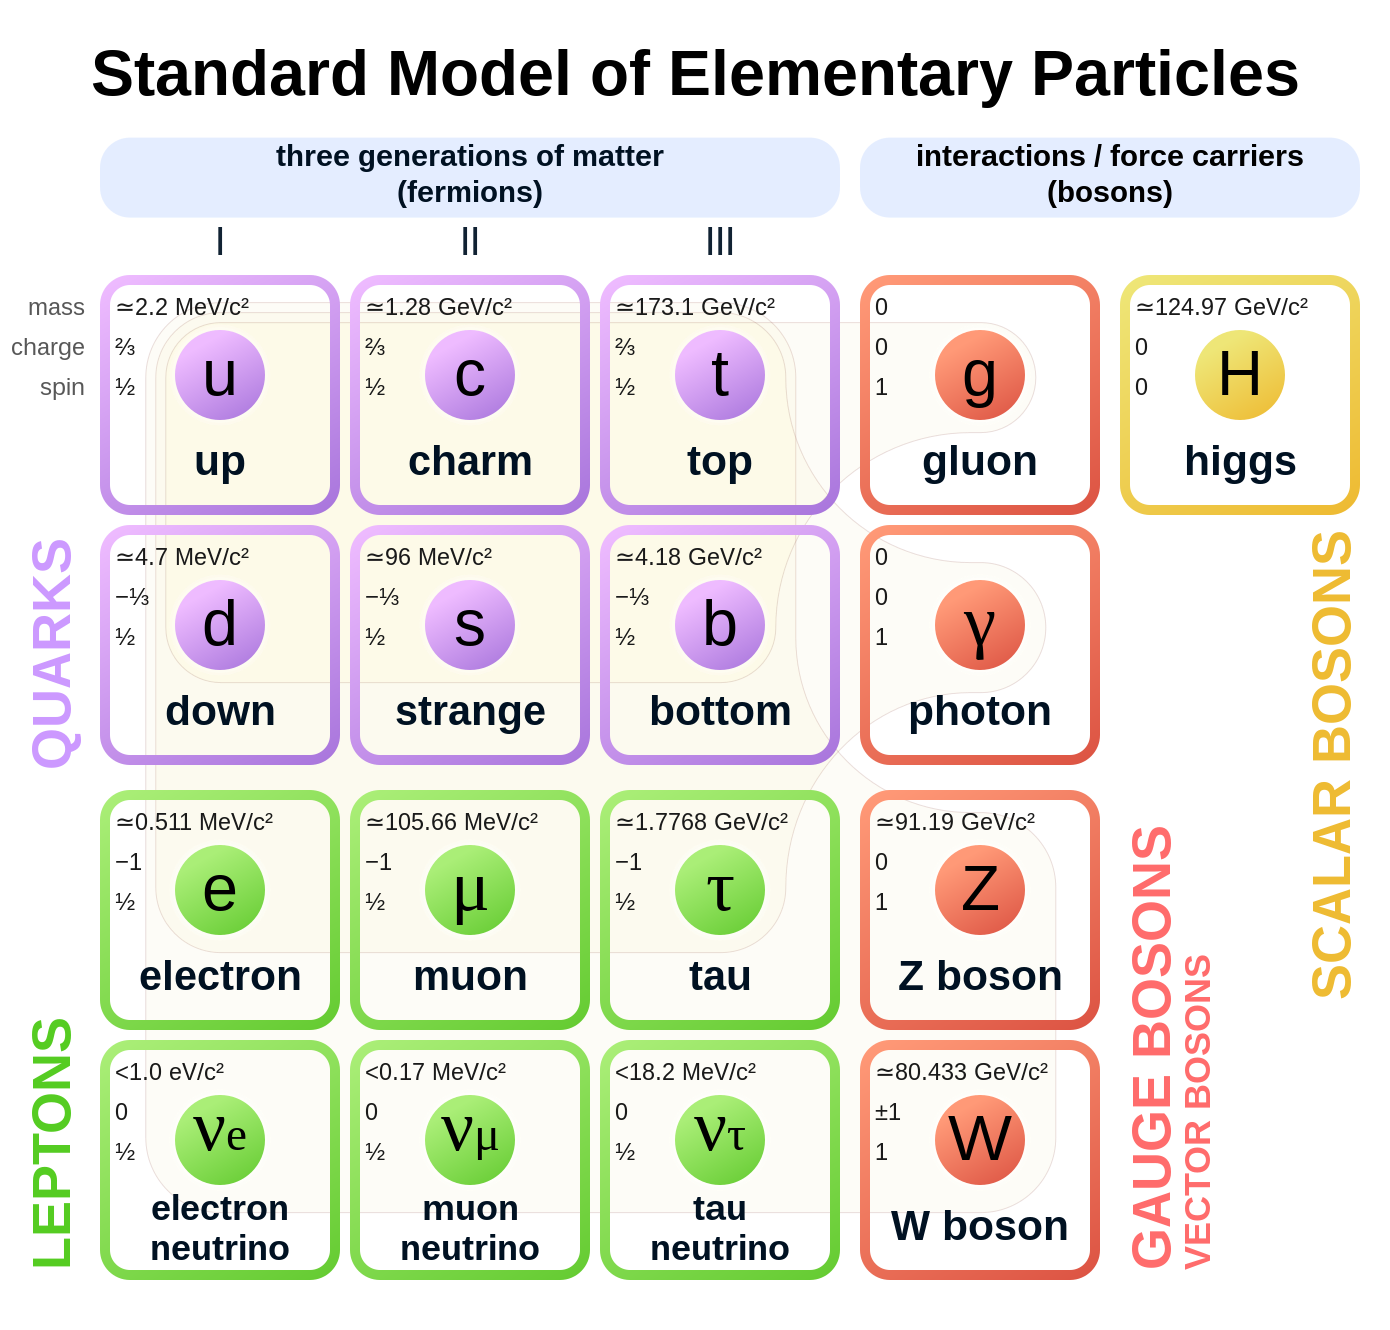
\includegraphics[width=\textwidth]{Figs/Chapter2/Standard_Model_of_Elementary_Particles.svg.png}\label{fig:StdModel}
	\caption{Classification of the elementary particles of the Standard Model, with the fermions on the left and the gauge/scalar bosons on the right. Figure taken from \cite{missmjStandardModelElementary2019}.}
	\label{fig:StdModel}
\end{figure}

Classically, a particle interacts with another via a field (for example, in electromagnetism, a positively charged particle generates an electric field that exerts an attractive/repulsive force on neighboring negative/positive charge). In QFT, fields are quantized, and the energy and momentum previously carried by the field are now conveyed by chunks, by quanta\footnote{Here, we present elementary particles as quanta  of their underlying field as if the particles could be separated/reduced from their field, which corresponds to the usual experimentalist's picture of QFT. In fact, the relation between particles and fields is slightly more subtle \cite{jaegerElementaryParticlesQuantum2021}.} \cite{serwayModernPhysics2004}. So in particle physics, interactions are described as an exchange of quanta or force-carrying particles of spin 1, known as \textit{(vector) gauge bosons}\footnote{They are called \textit{bosons} because, contrarly to the fermions, their intrinsic angular momentum (or spin) has an integer value.}\cite{braibantParticlesFundamentalInteractions2012}\cite{thomsonModernParticlePhysics2013}. Following the remarks in \Sec\ref{subsec:Theory}, the term "(\textit{vector}) \textit{gauge}" emphasizes here the fact that the boson arises from a gauge vector field and therefore a gauge symmetry. 

The most precise quantum field theory is the quantum electrodynamics (QED) that describes the interaction between charged particles and electromagnetic fields. It has been developped between 1947 and 1949 by Shin'-ichir$\bar{\text{o}}$ Tomonaga, Julian Schwinger, Richard P. Feynman and Freeman Dyson; only the first three received the 1965 Nobel Prize in Physics for their contributions\footnote{Unfortunately F. Dyson did not receive the Nobel Prize because i) his work was not considered as groundbreaking as the one of the three other laureates and ii) the Nobel Prize in a given field can only be awarded to organisation of maximum of three individuals \cite{schmidhuberEvolutionNationalNobel2010}.}. It is based on a U(1) local gauge symmetry\footnote{U(N) corresponds to the group of all unitary matrices to size $N \times N$. Thus, U(1) is a group containing all the continuous transformations of the phase of a complex number.}, that results into an interaction with charged particles mediated by massless photons. This continuous symmetry is associated to a conserved quantity, namely the electric charge. The dynamics of this interaction is given by the Lagrangian density of QED in \eq\ref{eq:LagrangianQED}.

\begin{equation}
\Lagr_{QED} = \underbrace{i \bar{\psi} \gamma^{\mu} \partial_{\mu} \psi}_{\substack{\text{electron} \\ \text{kinetic term}}} + \underbrace{e \bar{\psi} \gamma^{\mu} A_{\mu} \psi}_{\substack{\text{electron-photon} \\ \text{interaction term}}} - \underbrace{m \bar{\psi} \psi}_{\substack{\text{electron} \\ \text{ mass term}}} - \underbrace{\frac{1}{4} F_{\mu \nu} F^{\mu \nu}}_{\substack{\text{photon} \\ \text{kinetic term}}} 
\label{eq:LagrangianQED}
\end{equation}
where
\begin{itemize}
\item[$\bullet$] $\gamma^{\mu}$ Dirac matrices that express the vectorial nature of the interaction and $\mu$ is the Lorentz vector index,
\item[$\bullet$] $A_{\mu}$ the photon field,
\item[$\bullet$] $F_{\mu \nu} = \partial_{\mu} A_{\nu} - \partial_{\nu} A_{\mu}$ the field-strength tensor,
\item[$\bullet$] $e$ the coupling constant of QED which coincides with the electric charge of the electron-positron field,
\item[$\bullet$] $m$ the electron/positron mass,
\item[$\bullet$] $\psi$ the electron-positron spinor field,
\end{itemize}
with the Einstein's notation $x^{\mu} x_{\mu} = \sum\limits_{\mu=0}^{N} x^{\mu} x_{\mu}$ and the notations from \cite{thomsonModernParticlePhysics2013}.\\

Different terms appear in the expression of the Lagrangian density: the density of kinetic energy of the spinor field, the density of potential energy due to the interaction between the spinor and gauge fields, the mass energy of the spinor field\footnote{If the gauge boson is massive, there would be an extra mass term. Since the photon is massless, this term is null.}, the density of kinetic energy of the gauge boson (photon). The most interesting term is the second one, which describes the interaction between the charged particles and the photons. This interaction gives rise to different processes, usually pictured by Feynman diagrams. \Fig\ref{fig:FeynmanDiagramQED} shows the basic interaction vertex in QED.

\begin{figure}[H]
\begin{center}
\unitlength = 1mm
\subfigure[]{
	\begin{fmffile}{eegamma}
	\begin{fmfgraph*}(40,25)
	\fmfleft{i1,i2}
	\fmfright{o1}
	\fmflabel{$e^{-}$}{i1}
	\fmflabel{$e^{+}$}{i2}
	\fmf{fermion}{i1,v1}
	\fmf{fermion}{v1,i2}
	\fmf{photon,label=$\gamma$}{v1,o1}
	\end{fmfgraph*}
	\end{fmffile}
	\label{fig:eegamma}
}
\subfigure[]{
	\begin{fmffile}{lqlqgamma}
	\begin{fmfgraph*}(40,25)
	\fmfleft{i1,i2}
	\fmfright{o1}
	\fmflabel{$l, q$}{i1}
	\fmflabel{$\bar{l}, \bar{q}$}{i2}
	\fmf{fermion}{i1,v1}
	\fmf{fermion}{v1,i2}
	\fmf{photon,label=$\gamma$}{v1,o1}
	\end{fmfgraph*}
	\end{fmffile}
	\label{fig:lqlqgamma}
}
\end{center}
\caption{Interaction vertex in QED: (a) involving an electron and a positron, (b) generalized to any charged particles.}
\label{fig:FeynmanDiagramQED}
\end{figure}



Being the first quantum field theory developed, QED paved the way -- and even served as a template -- for all the subsequent quantum field theories. Therefore, it is not surprising that the form of Lagrangian density is the same for all the forces. 

Following the success of QED, attempts to develop a quantum field theory for the weak interaction started in the 1950s; none of them could provide a satisfactory description. In the same decade, important discoveries have been made: the Wu's\footnote{Awarded of the 1957 Nobel Prize.} (1956) and Goldhaber's (1957) experiments \cite{wuExperimentalTestParity1957}\cite{goldhaberHelicityNeutrinos1958} showed that the P- and CP-symmetries are violated by the weak interaction. These led to conclude that this force has a vector-axial vector structure, meaning that only interacts with left-handed chiral particles and right-handed chiral anti-particles. Meanwhile, a few physicists -- including Abdus Salam, Steven Weinberg, Schwinger and his PhD student Sheldon L. Glashow -- foresaw that the weak and electromagnetic forces might be two aspects of the same phenomenon. Thanks to the work of Chen Ning Yang and Robert Mills on the development of a generalized gauge theory in 1954, Glashow delivered the electroweak interaction in 1961, which was consolidated later in 1967 and 1968 by Weinberg and Salam\footnote{For their contribution, Glashow, Salam and Weinberg receive the 1979 Nobel Prize.} respectively. In this quantum field theory, the electromagnetic and weak forces are described within an unified framework; the weak interaction is based on the SU(2) gauge group\footnote{The S (for "special") refers to the group of all matrices whose determinant is equal to 1.}, three generators hence three gauge bosons: \rmWplus, \rmWminus and \rmZzero. These bosons exhibit two unique properties.  First, contrarly to all other gauge bosons, these ones have an enormous mass (m$_{\textrm{W}^{\pm}}$ = 80.377 \gmass and m$_{\textrm{Z}^{0}}$ = 91.1876 \gmass \cite{particledatagroupReviewParticlePhysics2022}), which explains why the weak force is such a short-range interaction. Second, the \rmWplusminus bosons can change the flavour of quarks and leptons. The trend (or the probability) of the flavour-changing is given by the \textbf{C}abibbo-\textbf{K}obayashi-\textbf{M}askawa\footnote{The Universe is unfair: similarly to Dyson for the QED, Nicolas Cabibbo (the pioneer of the CKM matrix) was not awarded with the 2008 Nobel Prize, while Makoto Kobayashi and Toshihide Maskawa were.} (CKM) matrix \cite{particledatagroupReviewParticlePhysics2022}\footnote{Mathematically speaking, this matrix relates the mass eigenstates to the weak eigentstates \cite{thomsonModernParticlePhysics2013}.} in \eq\ref{eq:CKMmatrix}.

\begin{equation}
V_{\textrm{CKM}} = 
\begin{pmatrix}
V_{\rm ud} & V_{\rm us} & V_{\rm ub}\\
V_{\rm cd} & V_{\rm cs} & V_{\rm cb}\\
V_{\rm td} & V_{\rm ts} & V_{\rm tb}
\end{pmatrix} = 
\begin{pmatrix}
0.97425 \pm 0.00022 & 0.2253 \pm 0.0008 & 0.00413 \pm 0.00049\\
0.225 \pm 0.008 & 0.986 \pm 0.016 & 0.0411 \pm 0.0013\\
0.0084 \pm 0.0006 & 0.040 \pm 0.0027 & 1.021 \pm 0.032
\end{pmatrix}\label{eq:CKMmatrix}
\end{equation}

Each matrix element provides the probability of transition from one flavour $i$ to another $j$ for quarks, but the same exists for the leptons and is called the \textbf{P}ontecorvo-\textbf{M}aki-\textbf{N}akagawa-\textbf{S}akata (PMNS) matrix. The elements of the PMNS matrix are slightly different from the CKM ones, though the structure and ordering are the same. 

Finally, concerning the strong interaction, we will see later in its dedicated sub-section, \Sec\ref{subsec:strongforce}. Patience!
\\


The overall picture of the Standard Model's elementary particles is presented in \fig\ref{fig:StdModel}. To this figure should be added the antiparticles. Indeed, to each particle -- fermion or boson -- corresponds an antiparticle that has the same properties, because of the CPT invariance, but with oppositely sign quantum numbers. Consequently, this also means that both CKM and PMNS matrices are the same for particles and antiparticles.

There is, however, one element of the table in the \fig\ref{fig:StdModel} that has not been discussed yet, that is the Higgs boson. It originates from the electroweak unification, so let us retrace our footsteps. The principles of gauge invariance inevitably give rise to massless gauge bosons, like the photons but not the massive \rmWplusminus, \rmZzero bosons. At the time of Glashow's electroweak model in 1961, no one could imagine a mechanism to generate the enormous masses of the weak interaction force-carriers. In the same year, Jeffrey Goldstone showed that the process of spontaneous symmetry breaking\footnote{This is the phenomenon in which a physical system perfectly symmetric breaks the symmetry without any external intervention. The most famous example of such process concerns the magnets. A material can be seen as an ensemble of microscopic magnets. If this material is ferromagnetic, all these magnets will tend to align with their neighbors.  When the temperature increases, the thermal motions start to disrupt this alignement until the material is not magnetized anymore. Conversely, as the material cools down, neighboring magnets starts to align until a critical temperature, when all the magnets lines up in one macroscopic direction. All directions are equivalent but the magnet has to choose one. This choice breaks the symmetic situation when all the directions are equivalent; this is a \textit{symmetry breaking}. Moreover, this choice is not influenced by any external agent, hence it is labelled as \textit{spontaneous}.\label{footnote:SpontaneousSymmetryBreaking}} leads to the existence of massless gauge bosons, called Goldstone bosons. Three years later, in 1964, three independent groups (Robert Brout and François Englert; Peter Higgs; Gerald Guralnik, Carl Richard Hagen, and Tom Kibble) demonstrated the Goldstone bosons could be absorbed by the massless gauge bosons to acquire a mass: this is the Higgs mechanism. It is only in 1967-68, that Weinberg and Salam put to use this mechanism within Glashow's model to generate the masses of \rmWplusminus and \rmZzero bosons. But this goes beyond the scope of the electroweak unification; with this mechanism, the mass of all elementary particles can be generated \cite{s.glashowInteractionsJourneyMind1990}. Incidentally, a new massive spinless particle, associated to a scalar field, emerges out of the Higgs mechanism: the Higgs boson. Its observation in laboratory was at the heart of Standard Model researches for decades until the 14th of March 2013 when the ATLAS and CMS experiments at the LHC at CERN announced the discovery of the Higgs boson \cite{cernNewResultsIndicate2023}\cite{kibbleEnglertBroutHiggsGuralnikHagenKibbleMechanismHistory2009}. The same year, Peter Higgs and François Englert receive the Nobel Prize for their contribution to the Standard Model.


\subsection{The strong force, a colourful interaction}
\label{subsec:strongforce}

Back in the 1960s, in the \say{glorious years} of particle physics, when physicists were submerged by the number of newly discovered \say{elementary} particles. Some of them were subject to the strong interaction, some were not; the former were referred as \textit{hadrons}\footnote{The expression originates from the Greek \textit{adros} meaning "thick and bulky".} and the latter as \textit{leptons}, as discussed in \Sec\ref{subsec:ParticleAndInteractions}. The hadrons were further sorted into two groups known as \textit{mesons} and \textit{baryons}\footnote{These terms originally refer to the mass of the particle: \textit{meson} comes from the Greek root \textit{meso} for "middle", that is in between the electron and proton masses; \textit{baryon} stem from Greek \textit{barys} for "heavy", suggesting any particle with a mass greater or similar to the one of the nucleons. Before the development of the quark model, the difference between the meson and the baryon was driven by their spin. The meson is a boson (integer spin values) where as the baryon is a fermion (half-integer spin values)\cite{s.glashowInteractionsJourneyMind1990}.}. But no one could draw out the underlying scheme between these particles and organise them into some kind of periodic table. There were some attempts though \cite{sakataCompositeModelNew1956}\cite{sakuraiTheoryStrongInteractions1960}; however the Mendeleev of particle physics is arguably Murray Gell-Mann. 

In 1961, he (and independently Yuval Ne'eman) proposed a classification scheme called the \textit{eightfold way} \cite{gell-mannEIGHTFOLDWAYTHEORY1961}\cite{neemanDerivationStrongInteractions1961}. At that time, eight spinless mesons, eight vector mesons of spin 1 and eight spin 1/2 baryons were known. In each of these octets, a pattern emerges when the hadrons are organized into groups/multiplets of roughly the same mass, a hint of the underlying structure of strong interaction. A year later, the eightfold way is updated and completed with a decuplet formed of spin-$\frac{3}{2}$ baryons. However, one of the ten members of the decuplet was not yet discovered but this periodic table of elementary particles can predict its properties: a mass near the 1675 \mmass, strangeness\footnote{A quantum number introduced by Murray Gell-Mann in 1953 order to explain the \textit{strange} behaviour of some particles, such as kaons \cite{gell-mannIsotopicSpinNew1953}. Any particle with a non-zero strangeness value is dubbed \textit{strange particle}.} of -3 and negatively charged, these are the characteristics of the \rmOmegaM. Its existence is confirmed experimentally in 1964 by the Alternating Gradient Synchrotron at the Brookhaven National Laboratory (BNL)\cite{barnesObservationHyperonStrangeness1964a}, validating the eightfold way once and for all.\\

Within the year of this discovery, Murray Gell-Mann (and independently Georges Zweig) unveiled the symmetry behind the eightfold way: there are no elementary hadrons; they are, in fact, all built out of more fundamental particles named \textit{quarks}. A composite object made of bosons can only lead to a boson whereas, formed by fermions, the object is either a fermion or a boson depending on the number of constituents involved. Hence, the quarks must be fermions of spin one-half, mesons are composed of an even number of quarks, baryons of an odd number. The smallest odd number is one, but i) it does not make sense to say that a composite structure is made of one constituent and ii) we will see later in \Sec\ref{subsubsec:confinement} that a system of one quark is physically impossible. Thus, mesons must be made out of two quarks and baryons out of three; these are the simplest imaginable arrangements. 

Originally, quarks exist in two flavours, \textit{up} ($u$) and \textit{down} ($d$), with fractional electric charges of $+2e/3$ and $-1e/3$ respectively. But an extra flavour was needed to explain the existence of strange hadrons: the strange quark, $s$, is born. It has the same properties as the $d$ quark, except that it is much heavier and it has an assigned strangeness number of -1. Any strange hadrons actually contains one to three $s$ quark, depending on their strangeness. Therefore, the predicted particle by the eightfold way, the \rmOmegaM, corresponds actually to the strangest hadron possible, a baryon with three strange quarks. 

With this particle comes the first difficulty of the quark model. Whatever the particle, it must obey the spin-statistics theorem. Quarks being fermions, the theorem states that two \textit{identical} fermions can not occupy the same quantum states simultaneously. However, \rmOmegaM is constituted of three exactly identical $s$-quark \cite{skandsIntroductionQCD2013}. This problem was overcome by Oscar W. Greenberg \cite{greenbergSpinUnitarySpinIndependence1964}, Moo-Young Han and Yoichiro Nambu \cite{hanThreeTripletModelDouble1965} in 1964-65 that introduced a new quantum number, the colour. Each quark comes in three colours or variants labelled as red ($r$), green ($g$) and blue ($b$). In this way, the spin-statistics problem is solved but new questions arises. If quarks carry a colour, hadrons are a mixture of colours. This is assumed to be an equal mixture of all the colours, such that the hadrons are colourless. How come? Why are there no coloured hadrons? 

Along the same line: in 1966, the main accelerator at the Stanford Linear Accelerator Center (SLAC) becomes operational and starts a program of deep inelastic scattering experiments in order to study the inner structure of nucleons. Based on James Bjorken's \cite{bjorkenCurrentAlgebraSmall2018} and Richard Feynman's  \cite{feynmanBehaviorHadronCollisions1988} calculations, the results of SLAC's experiments, in 1969, showed that the nucleons were made of point-like constituents of spin-$\frac{1}{2}$, dubbed \textit{partons}, behaving as free particles \cite{peskinIntroductionQuantumField2018}. The partons were nothing else than the quarks, and these observations established the validity the quark picture to the whole particle physics community. However, it is curious that the partons seem to behave as free particles but they can not escape the hadron.\\

These questions remain unanswered until 1973. This year had seen the development of Quantum Chromodynamics (QCD) -- the quantum field theory of the strong force -- and the discovery of two of its most salient properties, namely the colour confinement and the asymptotic freedom (discussed in \Sec\ref{subsubsec:confinement}). Fruit of the work of Harald Fritzsch, Heinrich Leutwyler and Murray Gell-Mann \cite{fritzschAdvantagesColorOctet1973}, the QCD describes the interaction between colour-charged objects, namely the partons. It is based on the gauge symmetry group SU(3), which has eight generators, giving rise to eight massless gauge bosons called \textit{gluons}, and imposes the conservation of colour. 

QCD is very similar to QED: the electric charge is replaced by a colour charge, antiparticles carry opposite colour charges, and the eight gluons take the role of the photon. The dynamics of QCD is given by the Lagrangian density in \eq\ref{eq:LagrangianQCD}.\\

\begin{equation}
\Lagr_{QCD} = \underbrace{i \bar{\psi}_{q}^{i} \gamma^{\mu} \delta_{ij} \partial_{\mu} \psi_{q}^{j}}_{\substack{\text{quark} \\ \text{kinetic term}}} + \underbrace{g_{s} \bar{\psi}_{q}^{i} \gamma^{\mu} t_{ij}^{a} A_{\mu}^{a} \psi_{q}^{j}}_{\substack{\text{quark-gluon} \\ \text{interaction term}}} - \underbrace{m_{q} \bar{\psi}_{q}^{i} \psi_{qi}}_{\substack{\text{quark} \\ \text{mass term}}} - \underbrace{\frac{1}{4} F_{\mu \nu}^{a} F^{a \mu \nu}}_{\substack{\text{gluon} \\ \text{kinetic term}}} 
\label{eq:LagrangianQCD}
\end{equation}
where, using the notations from \cite{skandsIntroductionQCD2013},
\begin{itemize}
\item[$\bullet$] $g_s^2 = 4 \pi \alpha_s$ with \alphaS the coupling constant of QCD,
\item[$\bullet$] $F_{\mu \nu}^{a} = \underbrace{\partial_{\mu} A_{\nu}^{a} - \partial_{\nu} A_{\mu}^{a}}_{\text{Abelian part}} + \underbrace{g_{s} f^{abc} A_{\mu}^{b} A_{\nu}^{c}}_{\text{non-Abelian part}}$ the field-strength tensor,
\item[$\bullet$] $\psi_{q}^{i}$ the quark field spinor with colour index $i$ such that $\psi_{q} = \left({\color{red}\psi_{qR}}, {\color{green}\psi_{qG}}, {\color{blue}\psi_{qB}} \right)^{\rm T} $,
\item[$\bullet$] $m_{q}$ the quark \textit{bare} mass induced by the Higgs mechanism,
\item[$\bullet$] $A_{\mu}^{a}$ the gluon field with colour index $a$,
\item[$\bullet$] $t_{ij}^{a} = \frac{1}{2} \lambda_{ij}^{a}$ and $\lambda^{a}$ the fundamental\footnote{The representation of a group is \textit{fundamental} when its generators are hermitian and traceless matrices. } representation of the generator of SU(3) associated to the colour index $a$,
\item[$\bullet$] $f^{abc}$ the structure constants of SU(3).\\
\end{itemize}

As in QED, the Lagrangian density can be expressed with four terms; the quark-gluon interaction is described by the second one. However, the field-strength tensor $F_{\mu \nu}^{a}$ here admits an extra term because the generators of SU(3) do not commute. The non-Abelian property of the gauge group of QCD gives rise to gluon-self interactions, as shown in the Feynman's diagrams of \fig\ref{fig:FeynmanDiagQCD}.

\begin{figure}[H]
\begin{center}
\unitlength = 1mm
\subfigure[]{
	\begin{fmffile}{qqg}
	\begin{fmfgraph*}(40,25)
	\fmfleft{i1,i2}
	\fmfright{o1}
	\fmflabel{$q$}{i1}
	\fmflabel{$\bar{q}$}{i2}
	\fmf{fermion}{i1,v1}
	\fmf{fermion}{v1,i2}
	\fmf{gluon,label=$g$, lab.dist=0.1w}{v1,o1}
	\end{fmfgraph*}
	\end{fmffile}
	\label{fig:qqg}
}
\subfigure[]{
	\begin{fmffile}{ggg}
	\begin{fmfgraph*}(40,25)
	\fmfleft{i1,i2}
	\fmfright{o1}
	\fmflabel{$g$}{i1}
	\fmflabel{$g$}{i2}
	\fmflabel{$g$}{o1}
	\fmf{gluon}{i1,v1}
	\fmf{gluon}{i2,v1}
	\fmf{gluon}{v1,o1}
	\fmfv{lab=$g_s$,lab.dist=0.15w}{v1}
	\fmfdot{v1}
	\end{fmfgraph*}
	\end{fmffile}
	\label{fig:ggg}
}
\subfigure[]{
	\begin{fmffile}{gggg}
	\begin{fmfgraph*}(40,25)
	\fmfleft{i1,i2}
	\fmfright{o1,o2}
	\fmflabel{$g$}{i1}
	\fmflabel{$g$}{i2}
	\fmflabel{$g$}{o1}
	\fmflabel{$g$}{o2}
	\fmf{gluon}{i1,v1}
	\fmf{gluon}{i2,v1}
	\fmf{gluon}{v1,o1}
	\fmf{gluon}{v1,o2}
	\fmfv{lab=$g_s^2$,lab.dist=0.15w}{v1}
	\fmfdot{v1}
	\end{fmfgraph*}
	\end{fmffile}
	\label{fig:gggg}
}
\end{center}
\caption{The three possible interaction vertices within the framework of QCD: (a) quark-gluon, (b) triple-gluon and (c) four-gluon interactions.}
\label{fig:FeynmanDiagQCD}
\end{figure}

Consequently to the self-interaction of QCD's force-carriers, gluons can not be colour neutral. To ensure colour conservation at the interaction vertex in \fig\ref{fig:qqg}, the gluon must carry a colour and an anti-colour charges. This calls for a revision of the term \textit{partons}: it corresponds to any colour-charged elementary particle, that is the quarks \textit{and} gluons. 

Furthermore, quarks are bound together inside hadrons through the exchange of gluons, but because of their self-interaction feature, gluons can radiate other gluons (\fig\ref{fig:ggg}); the latters can, in turn, split into a quark-antiquark pair (\fig\ref{fig:qqg}) or emit gluons again, and so on. The static picture of hadrons  with two or three quarks exchanging gluons turns out to be more complex, permeated in a \textit{sea} of quarks (and antiquarks) and gluons\footnote{An effect of the sea of quarks and gluons is the Bjorken scaling violation observed by the HERA experiment \cite{braibantParticlesFundamentalInteractions2012}\cite{thomsonModernParticlePhysics2013}.}. However, the elements inside the sea do not determine the quantum numbers or properties of the hadron, as opposed to the "original" quarks; for this reason, the latter are often refered as \textit{valence quarks}.

Finally, an incidental consequence of gluon's self-interaction is the running of the coupling constant. This can be understood by making a (anti)parallel with QED. Let us say we want to measure the coupling strength with a charged particle (an electron, for example). In QFT, the vacuum is not entirely empty, it contains pairs of particles and antiparticles that are constantly created and annihilated. Such a pair can also be formed by the cloud of \textit{virtual}\footnote{Certainly the most vague concept in particle physics. It appears in perturbation theory (see later) and an attempt for a definition could be: it corresponds to a theoretical particle wich exhibits the same properties as ordinary particles but not necessarily (for example, they do not satisfy the energy-momentum relation), and with a lifetime so short that it could never be observed experimentally.} photons surrounding the charged particle to be tested; in this case, it is said to \textit{polarise the vacuum}. An example of this process can be found in \fig\ref{fig:ChargeScreening}. The positively charged particle from the vacuum is attracted to the initial electron, leading in a screening effect similar to the one found in a dielectric material (\fig\ref{fig:Dielectric}). At large distance (or small energy), it is more difficult to penetrate inside the cloud of virtual particle-antiparticle pairs and to probe the initial charge, reducing the coupling strength. Conversely, at small distance (or large energy), the initial charge can be distinguished from the surrounding positively charged particles and the coupling strengthen. In QCD, the opposite happens.  Because gluons carry a colour charge, the initial colour of the particle to be tested (a quark) gets spread out, as depicted in \fig\ref{fig:ColourSpread}. Thus, an anti-screening effect occurs: the initial red-coloured quark spends most of its time coloured as blue or green, and the red colour charge is diluted in the surrounding cloud of partons. At large distance (or small energy), the initial quark $r$ is overly apparent for an incoming gluon $\bar{r}g$ or $\bar{r}b$; conversely, at small distance (large energy), the initial red quark -- likely converted into a green or blue quark -- is invisible to such a gluon, resulting in a weakening of the coupling strength. \\

\begin{figure}[t]
\begin{center}
\subfigure[]{
	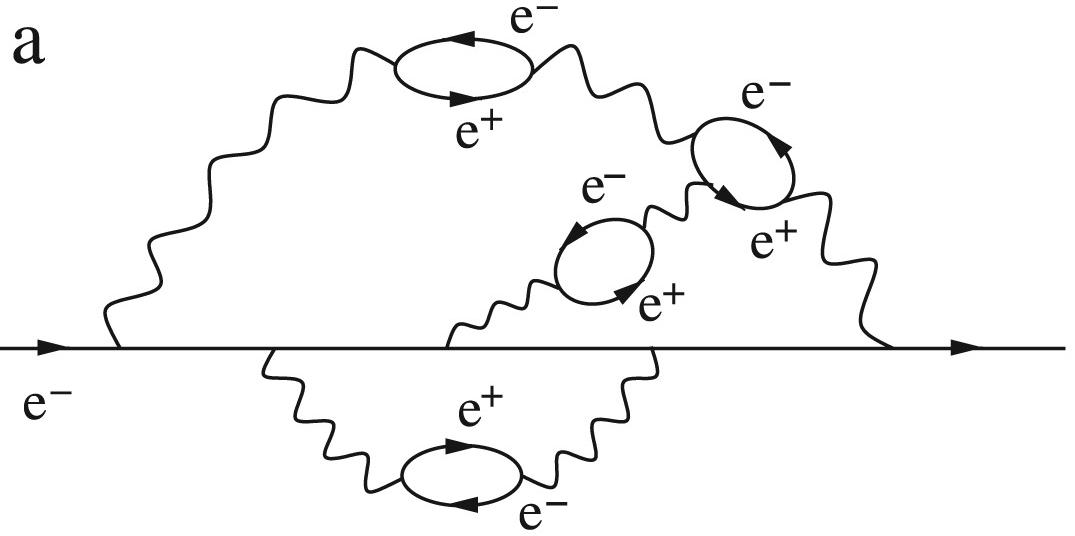
\includegraphics[height=0.25\textwidth]{Figs/Chapter2/1-s2.0-S0146641016300035-gr2_lrg}
	\label{fig:ChargeScreening}
}
\subfigure[]{
	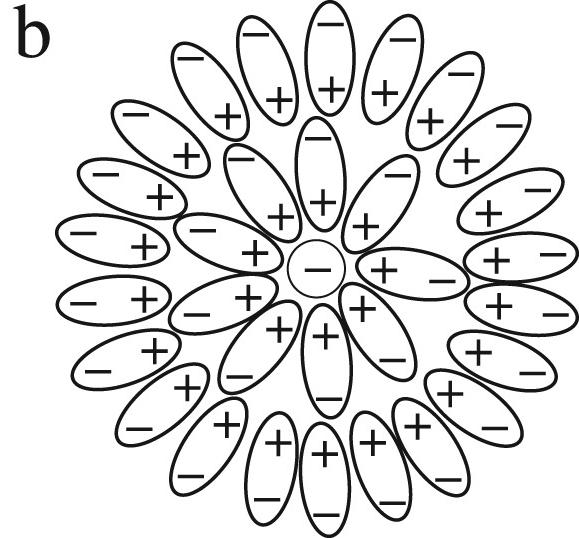
\includegraphics[height=0.25\textwidth]{Figs/Chapter2/1-s2.0-S0146641016300035-gr2bis_lrg}
	\label{fig:Dielectric}
}
\subfigure[]{
	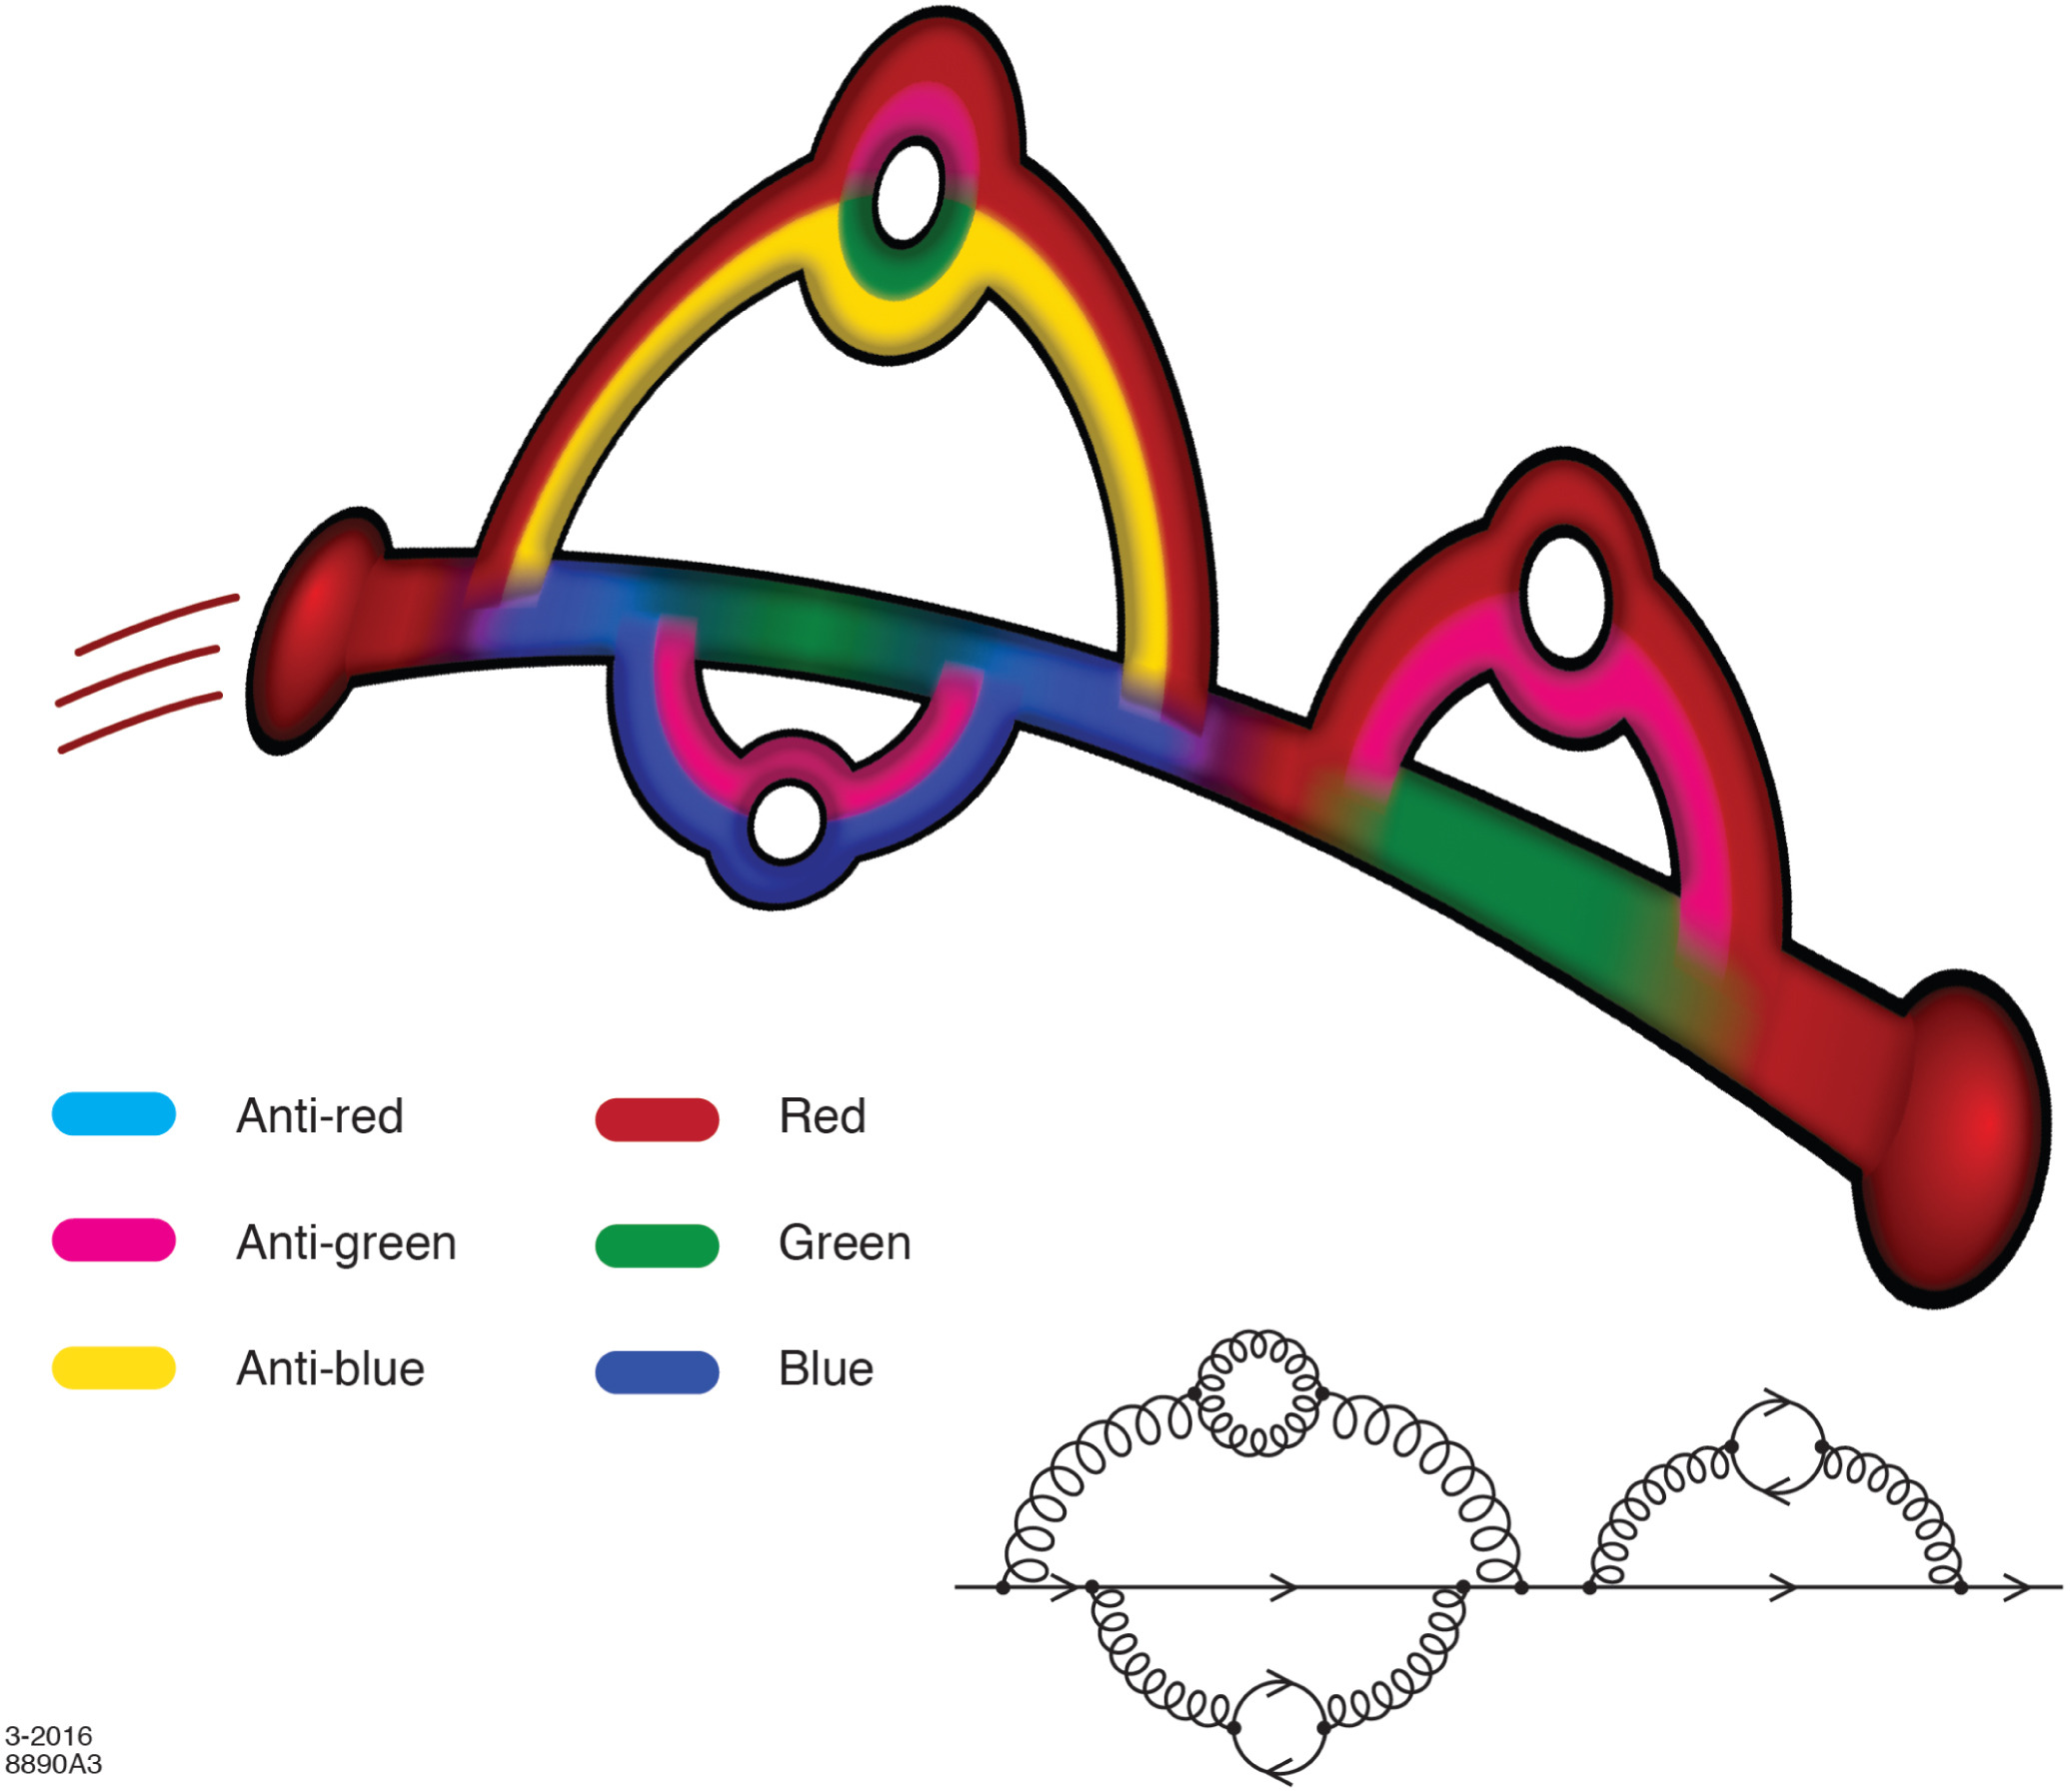
\includegraphics[width=0.8\textwidth]{Figs/Chapter2/1-s2.0-S0146641016300035-gr1_lrg.jpg}
	\label{fig:ColourSpread}
}
\end{center}
\caption{(a) screening effect of an electron in QED, induced ;(b) analogy with the screening effect in a dielectric material; (c) pictural representation of the colour spread of an initially red coloured quark. }
\label{fig:ProbingTestCHarge}
\end{figure}

%A physical picture often used to describe this effect is that a charged particle "polarizes the vacuum", and is "dressed" by a cloud of virtual photons and other charged particles. An electron will attract virtual positively charged particles out of the vacuum that effective screen the electric charge seen by an observer far away from the electron, reducing the size of the coupling. By bringing two charged particles to shorter distances (so they interact at a higher energy), the effective coupling between them is stronger because each charge penetrates the other's cloud, and so the virtual particles swarming in the quantum vacuum are less able to screen the bare charge of each charged particle. The reason for the name "screening" is that (in this picture) the quantum vacuum is screening the bare charge by surrounding it with virtual particles of the opposite charge. I should emphasize that this is a nice physical picture, but ultimately is just a set of words draped around a rigorous calculation of the running of the electromagnetic coupling with energy.

Before continuing, allow me to digress and finish with the different quarks within the QCD framework. The alert reader may have guessed that the story did not end with the strange quark. In 1964, James Bjorken and Sheldon Glashow introduced a new quark flavour: the charm quark. It is motivated by the idea of a quark-lepton symmetry\footnote{The term \textit{charm} is chosen for designating this fourth flavour because the definition found by Bjorken and Glashow in \textit{American Heritage Dictionnary}: "an action or formula thought to have magical power", implying magical power to restore the quark-lepton symmetry \cite{s.glashowInteractionsJourneyMind1990}.} at that time, there was four known leptons (electron, muon and their associated neutrinos) and three quarks. But the charm quark definitely comes into play in 1970 by Sheldon Glashow (again), John Iliopoulos and Lucinao Maiani to explain the strangeness-changing neutral currents\footnote{This is typically the case of the decay of a negative kaon to a negative pion with a neutrino and an anti-neutrino ($\rmKminus \rightarrow \piMinus \nu \bar{\nu}$). It is called a strangeness-changing neutral current because i) the strange particle (kaon) changed into an ordinary one (pion), and ii) there is no electric (or neutral) charge transfer between the hadrons to the leptons. This process was never observed in laboratory, as opposed to the strangeness-changing charged current: ($\rmKminus \rightarrow \piZero e^{-} \bar{\nu}_{e}$). To eliminate the strangeness-changing neutral currents, a new quark flavour needed to be introduced \cite{s.glashowInteractionsJourneyMind1990}.}. Its existence is validated by the observation of the first charmed hadron in 1974 by Burton Richter (SLAC)\cite{augustinDiscoveryNarrowResonance1974} and Samuel Chao Chung Ting (BNL)\cite{aubertExperimentalObservationHeavy1974}; both receive the 1976 Nobel Prize for that discovery. In parallel, a third generation of quark is introduced, in 1972 by Makoto Kobayashi and Toshihide Maskawa\footnote{For the discovery of, at least, a third family of quarks, they both receive the 2008 Nobel Prize.} to explain the observed CP violation. The particles composing this new family make their appearence in 1975, thanks to Haim Harari \cite{harariNewQuarkModel1975}, under the name of \textit{bottom} and \textit{top} quarks\footnote{Both belong to the same weak isospin doublet, as are the down and up quarks. To match the labelling of the first generation of quarks, the names \textit{bottom} and \textit{top} were chosen.}. Evidence of the bottom quark is found in 1977 by Leon M. Lederman at Fermilab \cite{herbObservationDimuonResonance1977}. Due to its large mass, the discovery of the top quark takes more time but ultimately occurs in 1995 by two groups at Fermilab \cite{cdfcollaborationObservationTopQuark1995}\cite{d0collaborationObservationTopQuark1995}.

\subsubsection{Running of \alphaS, colour confinement and asymptotic freedom}
\label{subsubsec:confinement}

\begin{figure}[h]
	\centering
	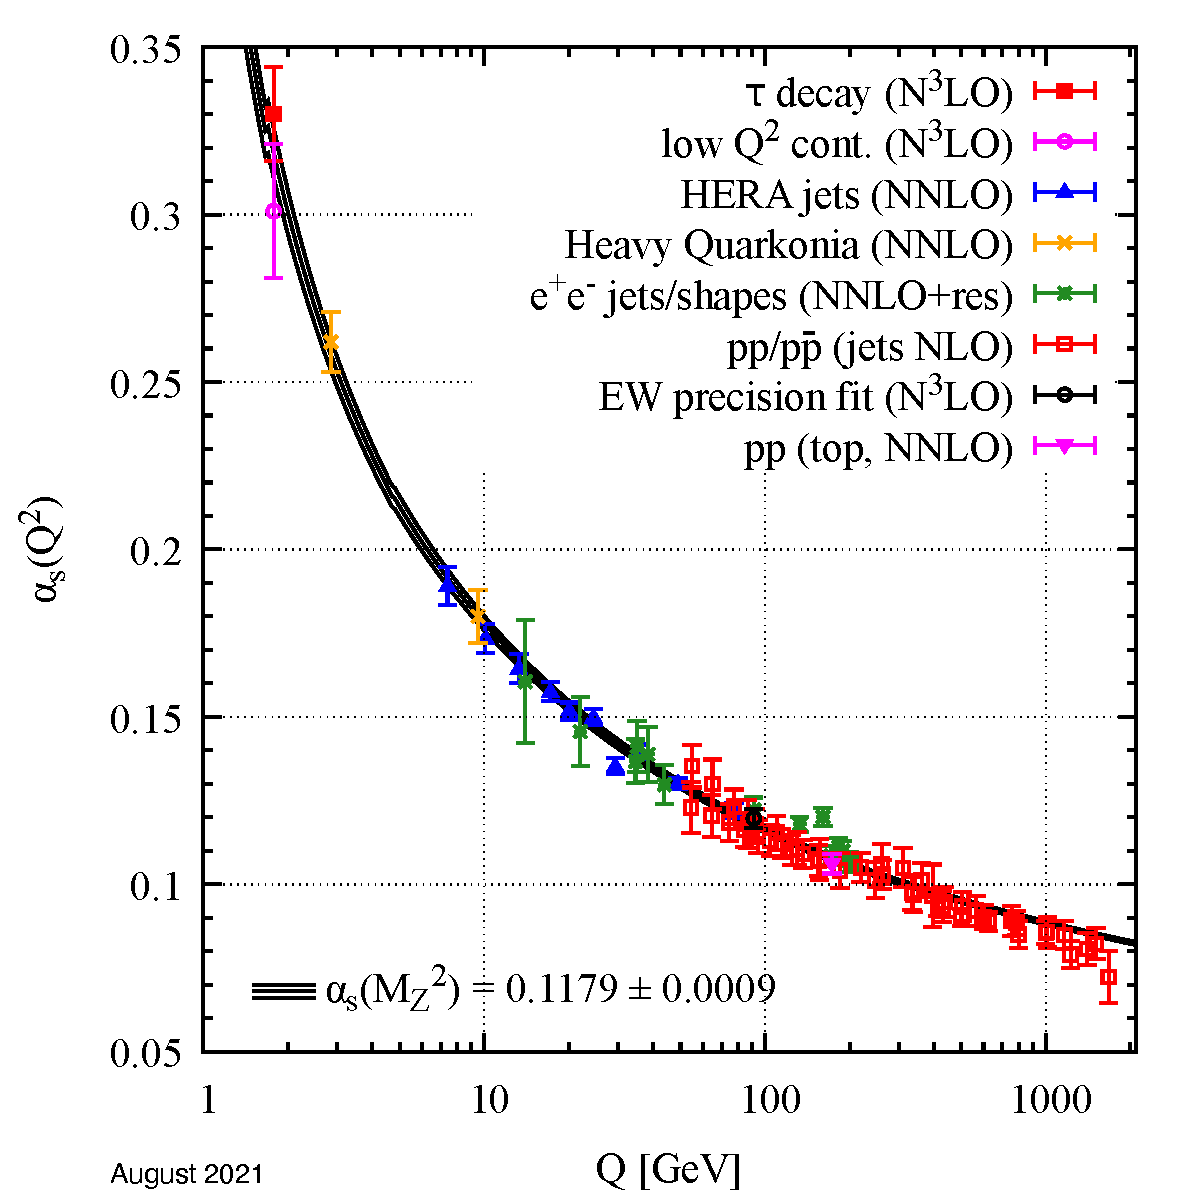
\includegraphics[width=0.8\textwidth]{Figs/Chapter2/alphas-v-Q-2021.pdf}
	\caption{Running of the coupling constant of the strong interaction, \alphaS, as a function of the energy transfer $Q$. The markers represent measurements based on perturbative calculation (the order of the perturbation development is indicated in parenthesis), the solid line corresponds to analytical prediction. Figure taken from \cite{particledatagroupReviewParticlePhysics2022}.}
	\label{fig:RunningAlphaS}
\end{figure}

\Fig\ref{fig:RunningAlphaS} shows the running of the coupling constant \alphaS of QCD as a function of the energy transfer $Q$. The strength of the interaction varies considerably, such that two regimes can be discerned: one at large $Q$ (or small distance) when the strong interaction is "weak" (\alphaS small), the other at small $Q$ (or large distance) when the coupling constant gets "strong" (\alphaS large). Usually, these two regimes are delimited by defining an energy scale, denoted as \LambdaQCD, at which $\alphaS \sim 1$. This corresponds to $\LambdaQCD \sim 200$ MeV\footnote{The definition of \LambdaQCD is convenient because it allows to classify quarks as a function of their mass hierarchy with respect to \LambdaQCD: $u$, $d$ and $s$ quarks belongs to the light-flavour sector ($\LambdaQCD \ll m_{s}, m_{u}, m_{d}$), the others are heavy-flavour quarks ($m_{t}, m_{b}, m_{c} \gg \LambdaQCD$).}. Far above this value, the contribution of high-order diagrams decreases with their order such that most of them can be neglected, and QCD predictions can be calculated easily -- or in the some cases, it simply renders the calculations possible -- using perturbation theory. In this case, we talk about perturbative QCD (pQCD).

As the energy transfer decreases, the coupling constant increases and perturbative calculations starts to diverge until the point where it becomes infinite, at \LambdaQCD. At this value or below, QCD is dominated by the contributions from high-order diagrams and can not be treated perturbatively anymore. The only way out is to perform analytical calculations, which is not possible due to the complexity of QCD. A more viable option is to resort to numerical calculations. A well-established technique is called \textit{lattice QCD}, where to each (space-time) point of the lattice/grid corresponds a spinor field representing the quarks possibly connected (or not) by links describing the gluon vector field. Although it provides some insights on non-perturbative physics aspects of QCD, it is extremely demanding in terms of computational power and time -- these two factors being strongly dependent on the lattice size.\\

A phenomenological approach of QCD, supported by lattice calculations, can also be followed by considering that the interaction potential between two quarks separated by a distance $r$ is approximated by\footnote{The expression of the potential is experimentally motivated by the ordering in the spectra of the charmonium ($c\bar{c}$) and bottomium ($b\bar{b}$) bound states \cite{thomsonModernParticlePhysics2013} \cite{martinParticlePhysics2017}.}
\begin{equation}
V(r) \approx - \frac{\alpha_{s}(r)}{r} + \kappa r,
\label{eq:QCDPotential}
\end{equation}
where the constant $\kappa$ is typically about 1 GeV/fm \cite{martinParticlePhysics2017}. The alert reader recognises the first term as the Coulombian-potential, similar to the one in QED; the second term corresponds to an elastic spring-type force. As illustrated in \fig\ref{fig:QCDPotential}, they describe two specific behaviours of the QCD interaction potential.

\begin{figure}[t]
	\centering
	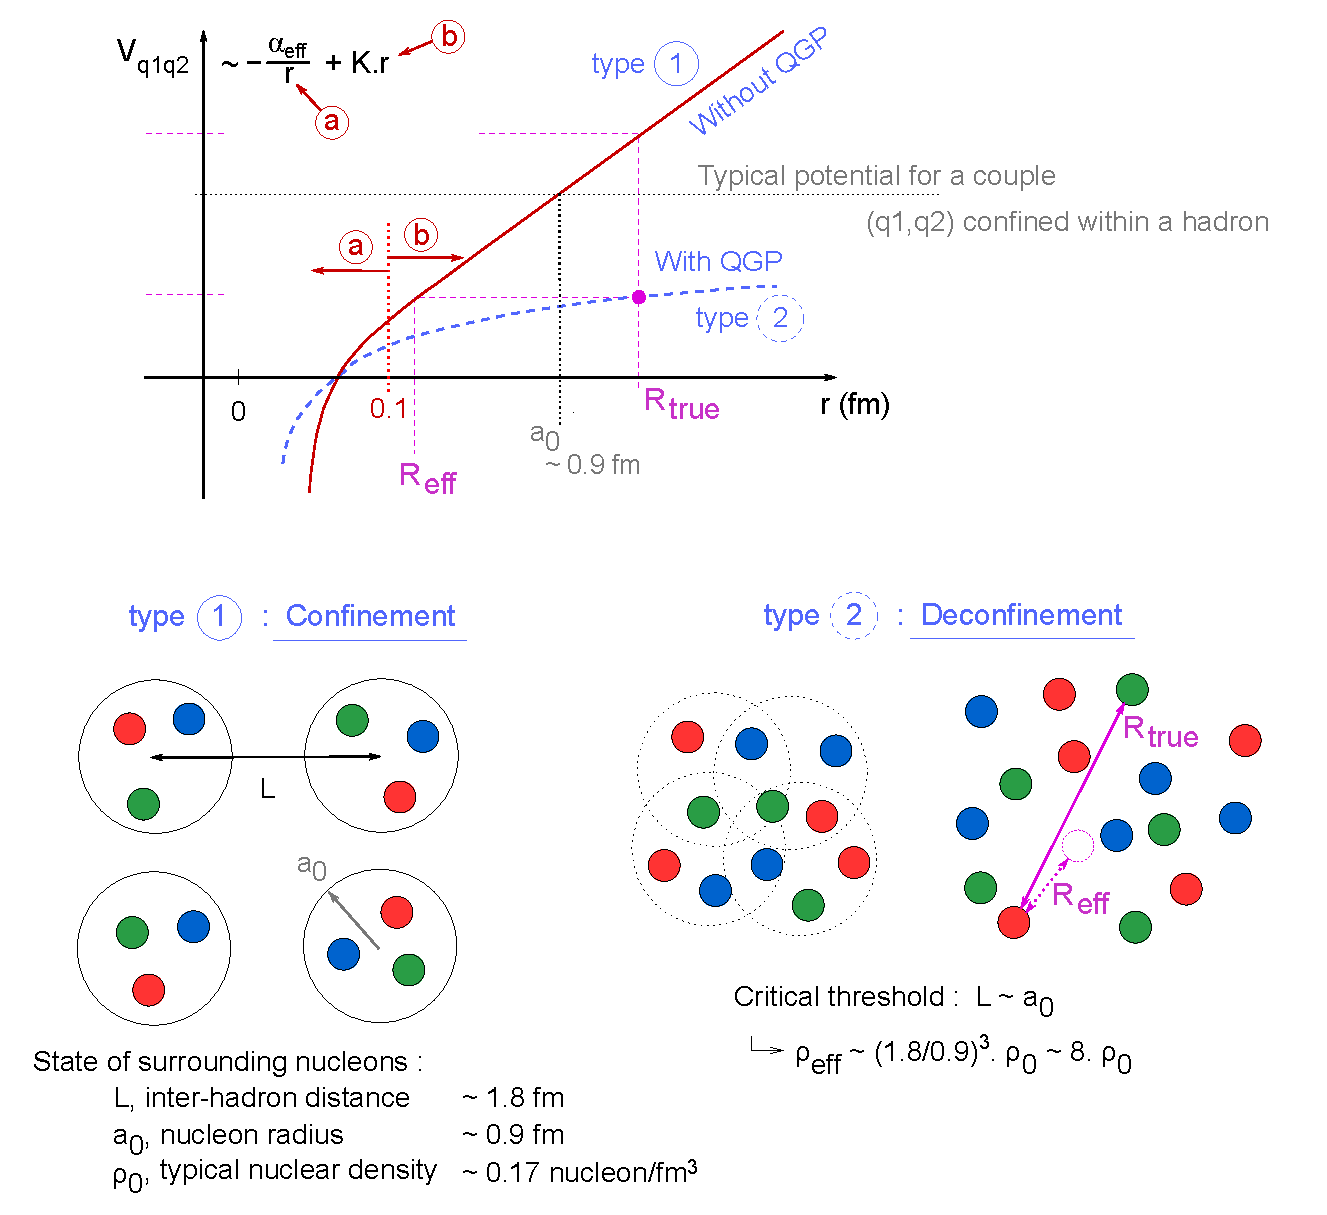
\includegraphics[width=0.9\textwidth]{Figs/Chapter2/GraphePotentiel.eps}
	\caption{QCD interaction potential between two coloured-objects (quark-quark or quark-antiquark) as a function of their separation $r$. Figure taken from \cite{maireProductionBaryonsMultietranges2011}.}
	\label{fig:QCDPotential}
\end{figure}

At small distance ($r \leq 0.1 \fm$), the Coulomb-type term dominates, the interaction potential diminishes asymptotically as the distance decreases; it is not divergent though, as \alphaS also varies. The quarks interacts less and less, and becomes quasi-free. This phenomenon, known as \textit{asymptotic freedom}, has been discovered by David Gross, Frank Wilczek in 1973 \cite{grossUltravioletBehaviorNonAbelian1973} and Hugh David Politzer in 1974 \cite{davidpolitzerAsymptoticFreedomApproach1974}, and sets the groundwork for the development of a quantum field theory of strong interaction, that is the QCD\footnote{In the early seventies, the common belief among the theoreticians was that quantum field theory fails to describe the strong interaction, and therefore it would be impossible to have a common mathematical framework for all the known forces (except gravity) \cite{s.glashowInteractionsJourneyMind1990}.}. Neither the electrostatic force between two charges nor the gravitational force between two masses exhibit this property; in these cases, the interaction gets weaker as the distance increases between the two objects.

Conversely, the second term takes the upper hand at $r \geq 1 \fm$, the force increases linearly with the distance between the two quarks, as if they were connected by an elastic or spring made of gluons. As the quarks are pulled away, the energy stored in the spring of gluons accumulates until it reaches the threshold to create a quark-antiquark pair\footnote{There is an alternative scenario: the energy stored in the spring of gluons continues to increase until it reaches the threshold to create not one but two quark-antiquark pairs. Obviously, this path -- which explains the production of one or several baryons from the vaccum -- demands more energy and thus is less probable to occur.}. This description is shown on \fig\ref{fig:QuarkFragmentation}. The spring tying together the initial $q_{i}\bar{q}_{i}$ pair ruptures and the accumulated energy is expended on producing a $q_{1}\bar{q}_{1}$ pair: the freshly created quark, $q_{1}$, binds with $\bar{q}_{i}$,  $\bar{q}_{1}$ with $q_{i}$. This process continues until all the $q\bar{q}$ pairs have a sufficiently low energy to combine into a hadron. Note that the initial quark-antiquark pair could be replaced by a pair of gluons and the process would still be the same. As a result, any colour-charged particle -- quark or gluon -- can not be found isolated; they must be confined in a colour-neutral object, such as meson and baryon\footnote{If there is (ordinarily...) no such thing as free parton, the same would be true for a colour-charged hadron. For this reason, baryons and mesons are colour-neutral structures.}. This phenomenon is refered as \textit{colour confinement}.


Interestingly enough, the quark confinement is analogous to the behaviour of a magnet. The latter consists of a north and south poles. If one tries to isolate one of the poles, for example, by cutting the magnet in half, this would only yield into two small magnets. Like the quarks, no one has ever seen an isolated magnetic pole (magnetic monopole).

\begin{figure}[t]
\begin{center}
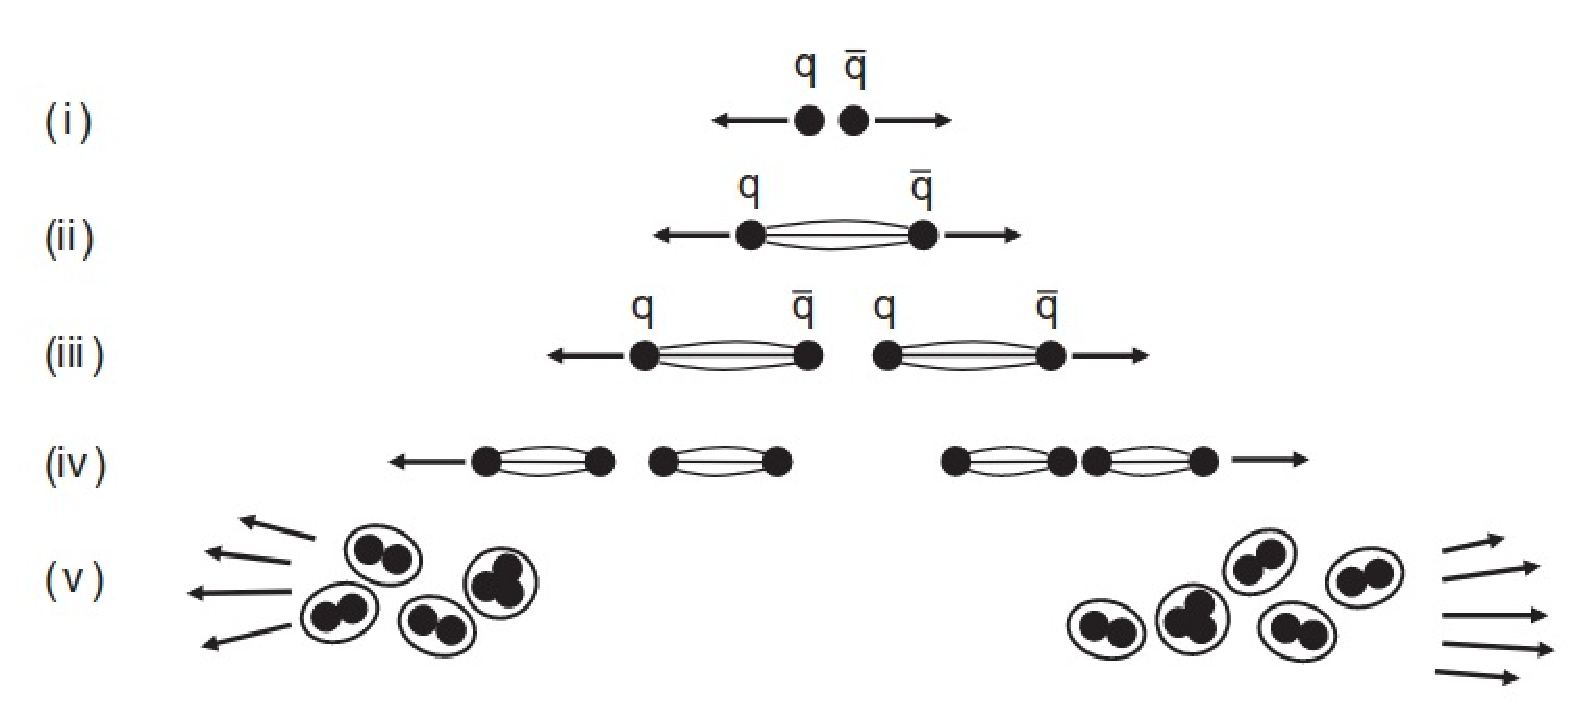
\includegraphics[width=0.9\textwidth]{Figs/Chapter2/Screenshot_20230220_214232.eps}
\end{center}
\caption{Schematic of the quark confinement: (i) the quark and antiquark are pulled away from each other;(ii) as they separated, the string of force tying together the pair stretches; (iii) the energy stored in the string now exceeds the necessary energy for creating a new quark-antiquark pair, the string will break and the two initial quarks will form smaller strings with the newly created pair;(iv) this process continues;(v) until all the quarks and antiquarks have a sufficiently low energy to form hadrons. Figure taken from \cite{thomsonModernParticlePhysics2013}.}
\label{fig:QuarkFragmentation}
\end{figure}

%On another note, hadrons can be classified as a function of their mass hierarchy of their quark constituent with respect to \LambdaQCD:
%\begin{itemize}
%\item[$\bullet$] Any hadron composed exclusively of up, down and strange valence quarks belongs to the \textit{light-flavour sector} ($\Lambda_{QCD} \gg m_{s}, m_{u}, m_{d}$)
%\item[$\bullet$] Any hadron containing, at least, one charm, bottom or top valence quark are members of the \textit{heavy-flavour sector} ($m_{t}, m_{b}, m_{c} \gg \Lambda_{QCD} $)
%\end{itemize}

\subsubsection{Chiral symmetry breaking}
\label{subsubsec:chiralsymmetrybreaking}

In \eq\ref{eq:LagrangianQCD}, the Lagrangian density of QCD was presented and split into four different terms. The quark and gluon kinetic energy and the quark-gluon interaction terms preserve the chiral symmetry, meaning that they leave the chirality of the quarks unchanged. The mass term, though, mixes the left- and right-handed particles:
\begin{equation}
m_{q} \bar{\psi}_{q}^{i} \psi_{qi} = m_{q} \left( \bar{\psi}_{q}^{i, L} \psi_{qi}^{R} + \bar{\psi}_{q}^{i, R} \psi_{qi}^{L} \right).
\label{eq:LagrangianQCDMassTerm}
\end{equation}

The quark mass, $m_{q}$, controls whether the chiral symmetry is broken or preserved. For massless quarks, this term is null hence left- and right-handed particles do not interact together; they would live, somehow, in two separate worlds. Consequently, every hadron would have a twin, identical in every point apart from the handedness: one  is left-handed, the other right-handed. In practice, the quarks have a finite mass but, for the light-flavour ones, it is sufficiently small to consider the chiral symmetry as an approximate symmetry. Therefore, chiral partners are expected to have slightly different masses. However, this is clearly not the case of the $\rho$ ($m_{\rho} = 770 \mmass$) and $a_{1}$ ($m_{a_{1}} = 1260 \mmass$) mesons, meaning that the chiral symmetry is much more broken than expected \cite{kochAspectsChiralSymmetry1997}. 

To be exact, it is \textit{spontaneously} broken\footnote{Well, it is also \textit{explicitly} broken but we will pass on that detail.}. This concept is visualised in \fig\ref{fig:ChiralSymmetryBreaking}. Returning to the example in the note \ref{footnote:SpontaneousSymmetryBreaking}, the continuous transition of the ferromagnet is characterised by an order parameter: the magnetisation. When the temperature is so high that the thermal motions disrupt the alignement of all the magnetic dipoles, the potential is symmetric and the minimum is centred at zero magnetisation (left \fig~\ref{fig:ChiralSymmetryBreaking}). As the temperature decreases and the magnet cools down, the symmetry of the potential is preserved but there are now two minima. The system (the ball) has to choose one, acquiring a non-zero magnetisation in the process, and hence breaking the symmetry (right \figs~\ref{fig:ChiralSymmetryBreaking}). 

\begin{figure}[h]
	\centering
	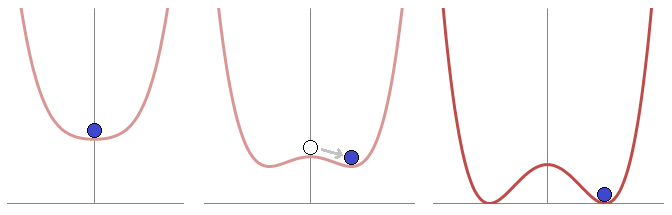
\includegraphics[width=\textwidth]{Figs/Chapter2/Spontaneous_symmetry_breaking_(explanatory_diagram).png}
	\caption{The left figure represents the shape of the potential at high energy, there is one minimum and it is centred on zero. Right figures: as the energy decreases and below a certain critical temperature, the ground state is no longer centred on zero but some distance away from it. Both ground states are equivalent, the system chooses one of them; this is a spontaneous symmetry breaking. The $x$-axis here represents the order parameter. Figure taken from \cite{ft2EnglishExplanatoryDiagram2012}.}
	\label{fig:ChiralSymmetryBreaking}
\end{figure}

The same process occurs for the chiral symmetry but, in this case, the order parameter is the \textit{chiral condensate}. This quantity, $< \psi_{q} \bar{\psi}_{q} > $ or $ < q \bar{q} >$, measures the coupling between left- and right-handed particles in vacuum. It was mentioned earlier that, in QFT, the vacuum is not empty but is composed of fleeting particle-antiparticle pairs that pop in and out. It could be that the Lagrangian density of QCD have an approximate chiral symmetry, but the vacuum does not. This means that particles with different handedness in the vacuum may (or not) interact together, depending the vacuum expectation value of the chiral condensate. If the $ < q \bar{q} >$ is null, the chiral symmetry is restored (left figure~\ref{fig:ChiralSymmetryBreaking}). Conversely, it is spontaneously violated when the chiral condensate is non-zero (right figures~\ref{fig:ChiralSymmetryBreaking}).

This symmetry was extensively studied by Yoichiro Nambu and Giovanni Jona-Lasinio in 1961 \cite{nambuDynamicalModelElementary1961}. In their model, the chiral condensate emerges from the passage of particles in the vacuum\footnote{In fact, the chiral condensate, and hence the spontaneous chiral symmetry breaking, is a consequence of the colour confinement \cite{peskinIntroductionQuantumField2018}.}; for that reason, the chiral symmetry breaking is qualified as \textit{dynamical}. Moreover, as the partons (inside a hadron) travel through the vacuum, they interact with the condensate and acquire an additionnal mass, the \textit{dynamical mass}\footnote{As opposed to the \textit{bare mass} stemming from the Higgs mechanism. It should be mentioned that nothing prevents the gluons to acquire also a dynamical mass. In this case, there would not be massless anymore.}. Predominant fraction of the hadron mass originates from this extra mass: for example, the proton mass sits $\sim 938$ \mmass and the bare mass of its quark constituents represents almost 10 \mmass, that is $\sim $ 1\% of proton mass.\\

On a side note, lattice QCD calculations predict that the chiral symmetry can be restored by heating or compressing matter. This is clear on \fig\ref{fig:ChiralSymmetryBreaking} where the chiral condensate vanishes as the temperature and/or density increases. In such conditions, the ordinary hadronic matter undergoes a phase transition, in which hadrons are only clothed by the bare mass of its constituents.

\begin{figure}[h]
\subfigure[]{
	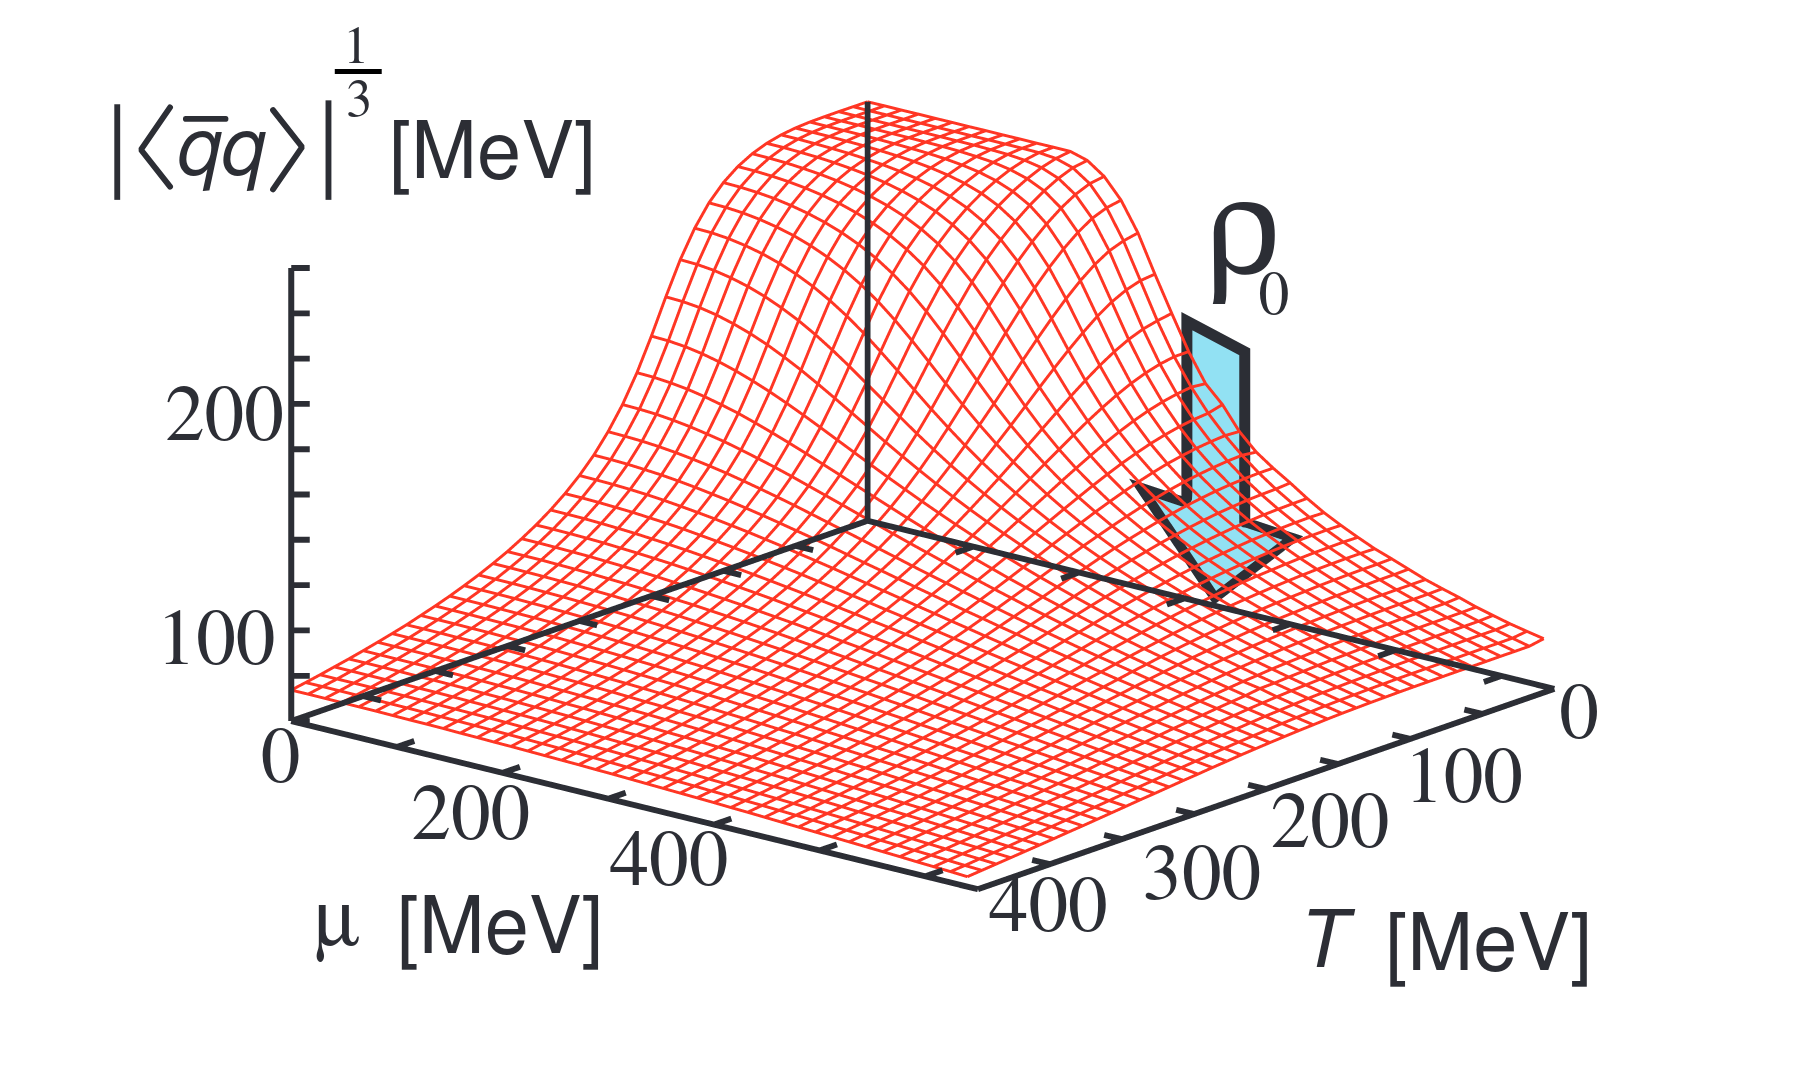
\includegraphics[width=0.50\textwidth]{Figs/Chapter2/ChiralCondensate.png}
}
\subfigure[]{
	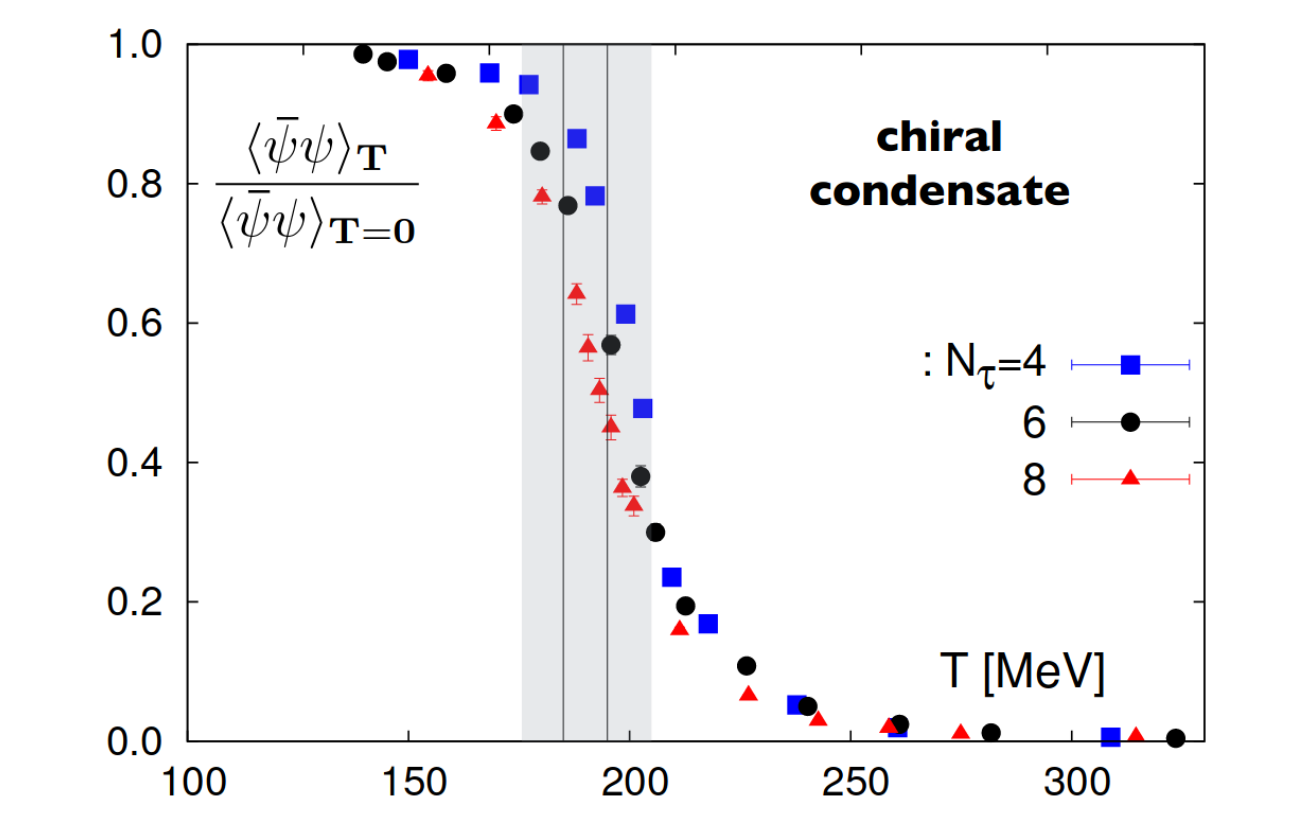
\includegraphics[width=0.50\textwidth]{Figs/Chapter2/ChiralCondensate2.png}
}
	\caption{Lattice QCD results on the evolution of the chiral condensate as a function of (a): the matter density (or the baryochemical potential $\mu$) and the temperature ($T$) \cite{muroyaLatticeQCDFinite2003}, (b): the temperature for different lattice points $N_{\tau}$ \cite{weiseChiralSymmetryStrongly2010}. The arrow on the left figure indicates the value of $\mu$ corresponding the ordinar nuclear density, $\rho_0$. The grey bands on the right figure indicate a range for the transition temperature.}
	\label{fig:ChiralSymmetryBreaking}
\end{figure}

\subsubsection{The QCD-phase diagram}
\label{subsubsec:QCDphasediagram}

In addition to the chiral phase transition, another one comes onto stage as the temperature increases. The \fig\ref{fig:QCDEnergyDensity} shows the predicted evolution of the pressure, energy density and entropy density for a hadron gas as a function of the temperature of the medium. The properties of the gas change rapidly when the temperature reaches $T_{c} = 154$ \mev, indicating the liberation of many degrees of freedom. In this case, these are the partons -- ordinarly confined within hadrons -- that now undergoes a \textit{deconfinement} transition and becomes quasi-free. 

I write \textit{quasi}-free because even at $T \sim 400 $ \mev, the energy density does not reach the ideal gas limit. As a consequence, the quarks and gluons are still interacting but weakly. Due to this shared similarity with the plasmas, this new state of hadronic matter is dubbed \textit{quark-gluon plasma} (QGP). Note that, because the coupling between the partons decreases with the increasing momentum transfer and temperature (asymptotic freedom), the energy density will ultimately overlap with the ideal gas limit but at much larger temperature though. \\

\begin{figure}[h]
	\centering
	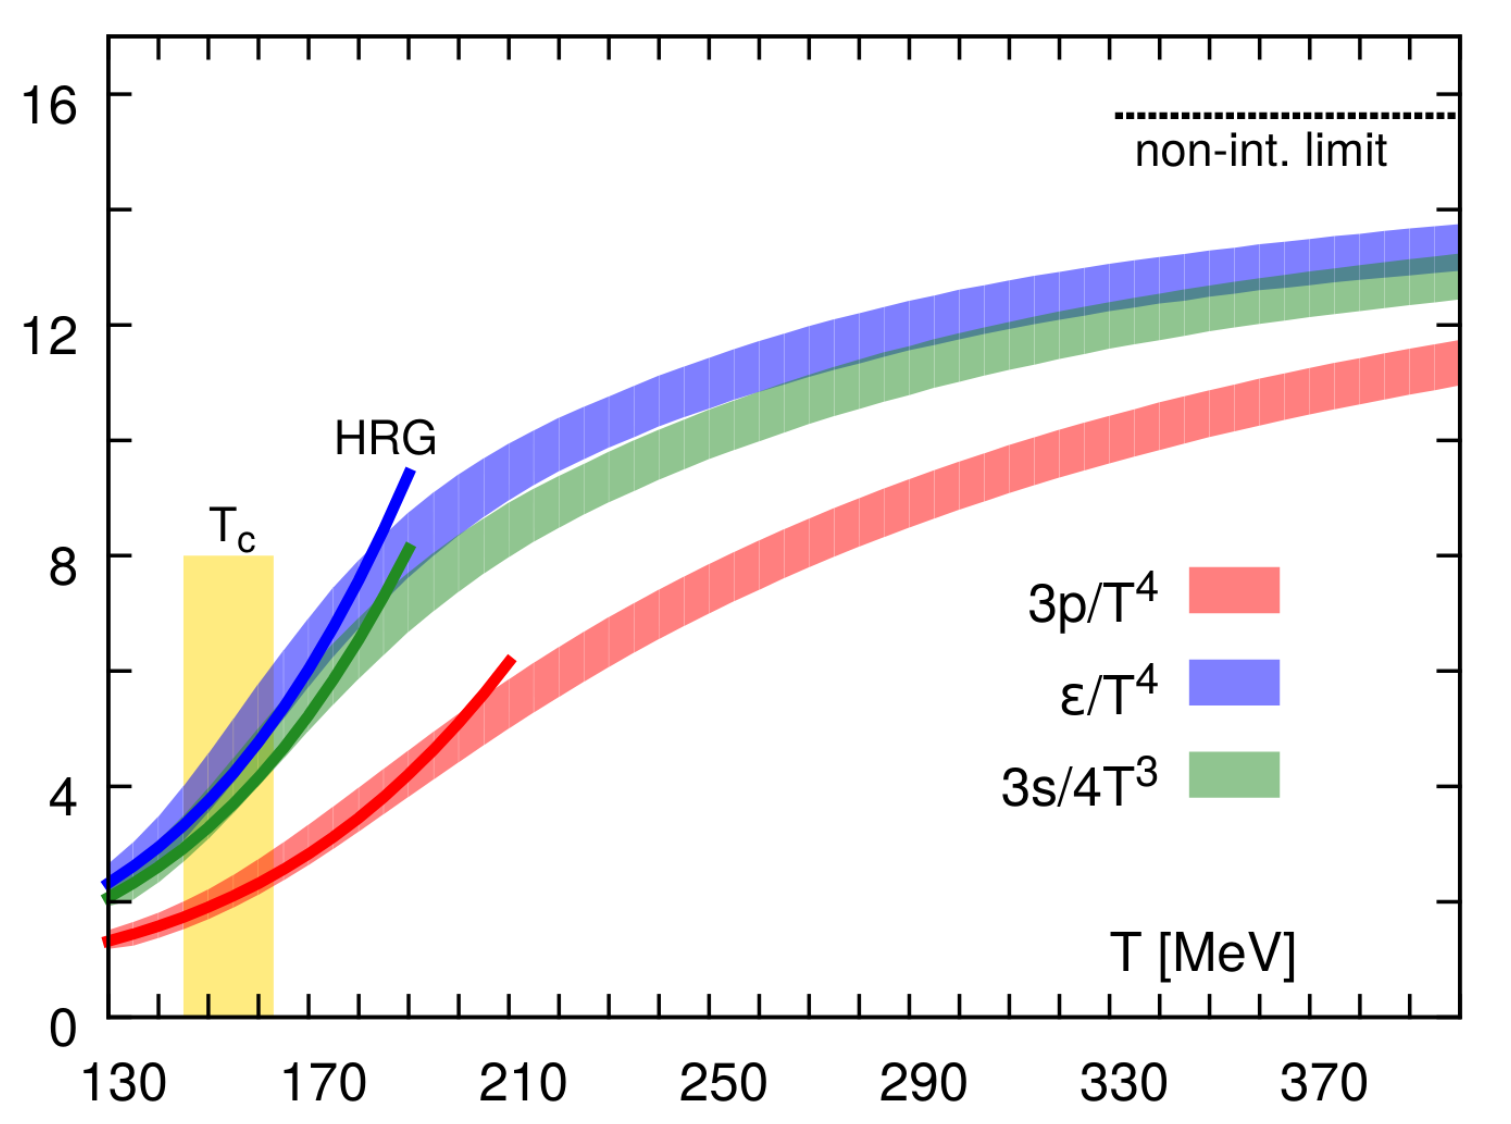
\includegraphics[width=0.7\textwidth]{Figs/Chapter2/Pressure_energy_entropy.png}
	\caption{Lattice QCD calculations of the pressure ($p$), energy density ($\epsilon$) and entropy density ($s$) normalised to the fourth (third, for the last quantity) power of temperature. The solid lines represent the prediction of the hadron resonance gas (HRG) model, the black dashed line indicates the energy density in the limit of an ideal gas. The transition temperature $T_{c}$ is equal to $154 \pm 9$ \mev. It should be emphasised that these predictions have been obtained assuming a zero net baryon density. Figure taken from \cite{bazavovEquationStateFlavor2014}.}
	\label{fig:QCDEnergyDensity}
\end{figure}

The \fig\ref{fig:QCDPhaseDiagram} provides the full QCD phase diagram. As it can be seen, there are two general ways to form a quark-gluon plasma: either one increases the temperature, or one increases the net baryonic density by compressing hadronic matter. The above phase transition corresponds to the former: by heating up the system at (almost) zero net baryon density, ordinary nuclear matter transforms first into a hadron gas and then undergoes a phase transition towards a QGP. This is what someone would see if he/she could rewind the videotape of the time-evolution of the Universe, from nowadays to a few \musec after the Big Bang. In the latter, the ordinary nuclear matter at relatively low temperature acquires, by compression, a larger and larger baryon density until the system transforms into a QGP. This state of matter is supposed to be present in the core of neutron stars\cite{annalaEvidenceQuarkmatterCores2019}, with potentially a colour superconductor behaviour \cite{alfordQCDFiniteBaryon1998}.

\begin{figure}[h]
	\centering
	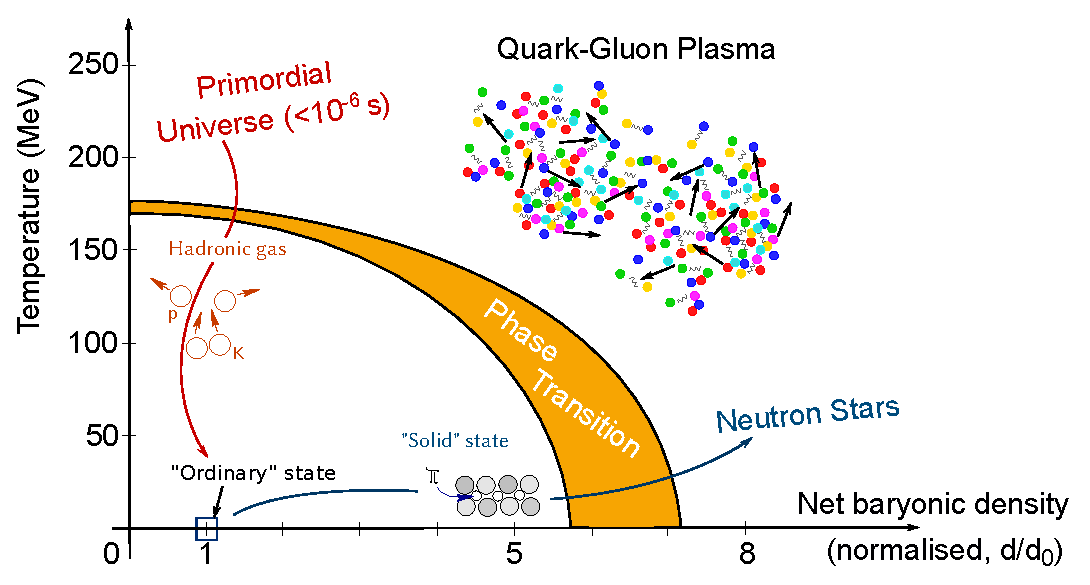
\includegraphics[width=\textwidth]{Figs/Chapter2/DiagrPhase.eps}
	\caption{Schematic representation of the QCD phase diagram as a function of the temperature and the net baryonic density. The latter is normalised to the net baryon density of ordinary nuclear matter. Figure taken from \cite{mairePhaseDiagramQCD2015}.}
	\label{fig:QCDPhaseDiagram}
\end{figure}

There is a profund difference in the nature of the phase transition between the one in the high-temperature region and the other with a high baryon density. Similarly to chiral transition on \fig\ref{fig:ChiralSymmetryBreaking}, the \fig\ref{fig:QCDEnergyDensity} shows a smooth evolution from one phase to another, indicating a second order --- or at least, a crossover --- phase transition \cite{philipsenQCDEquationState2013}. In contrast, the high baryon density driven evolution is expected to be more abrupt, more sharp as when ice melts to turn into water. This corresponds to a first order transition. It follows that there must be a critical point somewhere in the middle of the phase diagram, joining the first and second (or crossover) phase transitions \cite{stephanovQCDPhaseDiagram2005}. Its precise location is currently unknown, as no singularities have been observed yet.


\section{The Quark-Gluon Plasma}
\label{sec:QGP}

Each field of research has its pioneers and the study of the quark-gluon plasma is no exception. The first one was arguably Rolf Hagedorn, who approached the particle production making use of statistical physics. This endeavor led ultimately to the invention of the statistical bootstrap model (SBM) in 1964. At that time, a large number of massive resonances were observed, and this model provided a successful production mechanism for these particles\footnote{The statistical bootstrap model considers a gas of interacting hadrons, composed of all possible particles and their resonances, in a heat bath. If several light hadrons and/or resonances get compressed into a smaller volume, they could themselves be considered as a highly excited and massive resonance (also called fireball). Thus, the hadron gas rather corresponds to a gas of fireballs, that can also become a fireball in itself if compressed. This description provided an explanation for the mass spectrum of hadronic states.}. However, this description was conceived before the development of the quark model. When the quarks were finally considered as the elementary building blocks of hadrons, an extension of SBM was called for \cite{rafelskiMeltingHadronsBoiling2015a}.

The mutation of the statistical hadronisation model was achieved by the father of SBM and Johann Rafelski, between 1977 and 1980. This process led to a new paradigm. It was realised that, at a certain temperature, hadrons are melting to form a new phase composed of boiling quarks: the quark-gluon plasma. Although this concept was already intuited before by numerous physicists -- including Peter Carruthers in 1974 \cite{rafelskiMeltingHadronsBoiling2015} or George F. Chapline and Arthur K. Kerman in 1978 \cite{chaplinePossibilityMakingQuark1978} --, it was only approached qualitatively.

Nevertheless, Chapline and Kerman were the first ones to make the connection between the QGP and (relativistic) heavy-ion collisions. The same year, this point is addressed quantitatively by Siu A. Chin\cite{chinTransitionHotQuark1978a} and later refined in a paper by James D. Bjorken in 1983 \cite{bjorkenHighlyRelativisticNucleusnucleus1983}. In this renowned publication, Bjorken presents an analytical solution for one-dimensional relativistic hydrodynamics in heavy-ion collisions, as well as the space-time evolution of the QGP at mid-rapidity (\textit{Bjorken scenario}), laying down the foundations for the research programme at CERN.\\

Starting in 1986, a vast number of heavy ion experiments emerges at the CERN's Super Proton Synchrotron (SPS): WA85, NA36, NA35, Helios-2, NA38, WA80, and their future descendants \cite{satzSPSHeavyIon2004}. At first, $^{16}$O and $^{32}$S nuclei were accelerated at 200 \gev (per nucleon) until 1995, when the SPS switched to $^{208}$Pb beams with an energy per nucleon of 158 \gev. In a press conference held in February 2000, CERN reports to have \say{compelling evidence that a new state of matter has been created. The new state of matter found in heavy-ion collisions at the SPS features many of the characteristics of the theoretically predicted quark-gluon plasma} \cite{NewStateMatter2023}. This announcement marks a turning point for QGP research: partonic matter is not a mere theoretical concept anymore; it becomes real, tangible and measurable. 

The Relativistic heavy-ion Collider (RHIC) at BNL enters in operation in the next few months, with its four experiments -- BRAHMS \cite{arseneQuarkGluonPlasma2005}, PHOBOS \cite{alPHOBOSPerspectiveDiscoveries2005}, PHENIX \cite{phenixcollaborationFormationDensePartonic2005}, STAR \cite{starcollaborationExperimentalTheoreticalChallenges2005} -- dedicated to observe and characterise the QGP under different observables. In April 2005, BNL holds a press conference in order to present the results of the RHIC experiments, and by doing so, confirms the existence of "a new type of nuclear matter" \cite{ludlamHUNTINGQUARKGLUON2005}.

Nowadays, the study of the QGP is mainly centred around two accelerators: the RHIC at BNL and, since 2009, the Large Hadron Collider (LHC) at CERN. Alike RHIC, the latter also has four experiments: ATLAS, CMS, LHCb and ALICE. Although, they all have a heavy-ion research programme, ALICE is specifically designed to analyse the QGP. Concretely, it pursues the exploration of the QCD phase diagram and the characterisation of this new state of matter initiated at the RHIC, but at much higher energies. For comparison, the LHC delivers Pb-Pb collisions at a centre-of-mass energy per nucleon \sqrtSnn = 2.76 and 5.02 \tev, and Xe-Xe collisions at \sqrtSnn = 5.44 \tev. This is, at least, twenty times more energetic than at the RHIC. The LHC accelerator, as well as the ALICE collaboration, are presented in the next chapter, \chap\ref{chap:ALICE}. 


\subsection{The time evolution of a heavy-ion collision}
\label{subsec:BjorkenScenario}

We timidly started above to raise the question of how a heavy-ion collision leads to the formation of the QGP? This point was addressed by Bjorken in his scenario of the same name. Although the current description turns out to be more complex than anticipated, the Bjorken scenario still provides the key steps of the QGP formation process. The following discussion is structured around the \figs\ref{fig:PbPbSimu} and \ref{fig:QGPEvol}\\

A facility, such as the LHC or RHIC, accelerates heavy nuclei to ultra-relativistic speed. At the LHC energies, the Pb nuclei in each beam are accelerated to, at least, 1.38 \tev\footnote{The least energetic Pb-Pb collision available at the LHC being \sqrtSnn = 2.76 \tev, each beam carries 1.38 \tev per nucleon.}, which corresponds to a Lorentz factor $\gamma$ of about 1500. Consequently, as Bjorken argued \cite{bjorkenHighlyRelativisticNucleusnucleus1983}, even though the partons involved in the collision carry a tiny fraction of the incident beam energy, the nuclei are so extremely boosted that the space-time evolution of the system should be the same in all centre-of-mass frames near central rapidity, and thereby the particle yield should be flat as a function of rapidity, defining a central plateau structure for particle production. Moreover, at such energies, the nuclei are not stopped but rather continue to recede in opposite direction with respect to the collision point; this is the \textit{Bjorken regime} or \textit{transparency regime} and corresponds to net baryonic density close to zero\footnote{As opposed to the \textit{Landau regime} or \textit{stopping regime}, where the nuclei are completely stopped in frontal collisions. It occurs only for collisions at centre-of-mass energies up to a dozen of \gev per nucleon pair. These two regimes actually relates to the two different QGP phase transition: either by heating the system (Bjorken scenario) or compressing it (Landau scenario).}. Another implication is that, because of the length contraction, the nucleus looks like a highly-contracted pancake at mid-rapidity, as can be seen on \fig\ref{fig:PbPbSimu}.\\

\begin{figure}[h]
	\centering
	\hspace*{-2cm}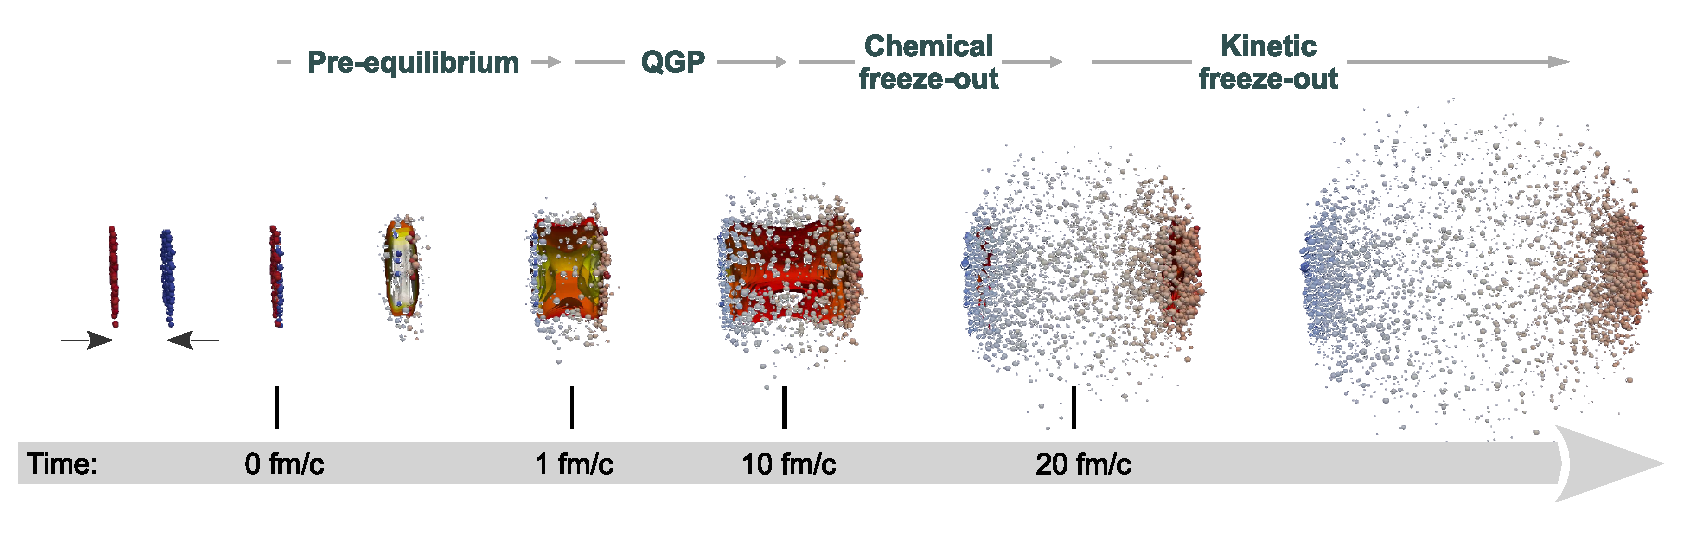
\includegraphics[width=1.35\textwidth]{Figs/Chapter2/PbPbCollision.eps}
	\caption{Simulation of the time evolution of a heavy-ion collision, rendered in seven pictures. Figure originally created by Hannah Petersen, taken from \cite{bernhardBayesianParameterEstimation2018} and modified by the present author.}
	\label{fig:PbPbSimu}
\end{figure}

\begin{figure}[h]
	\centering
	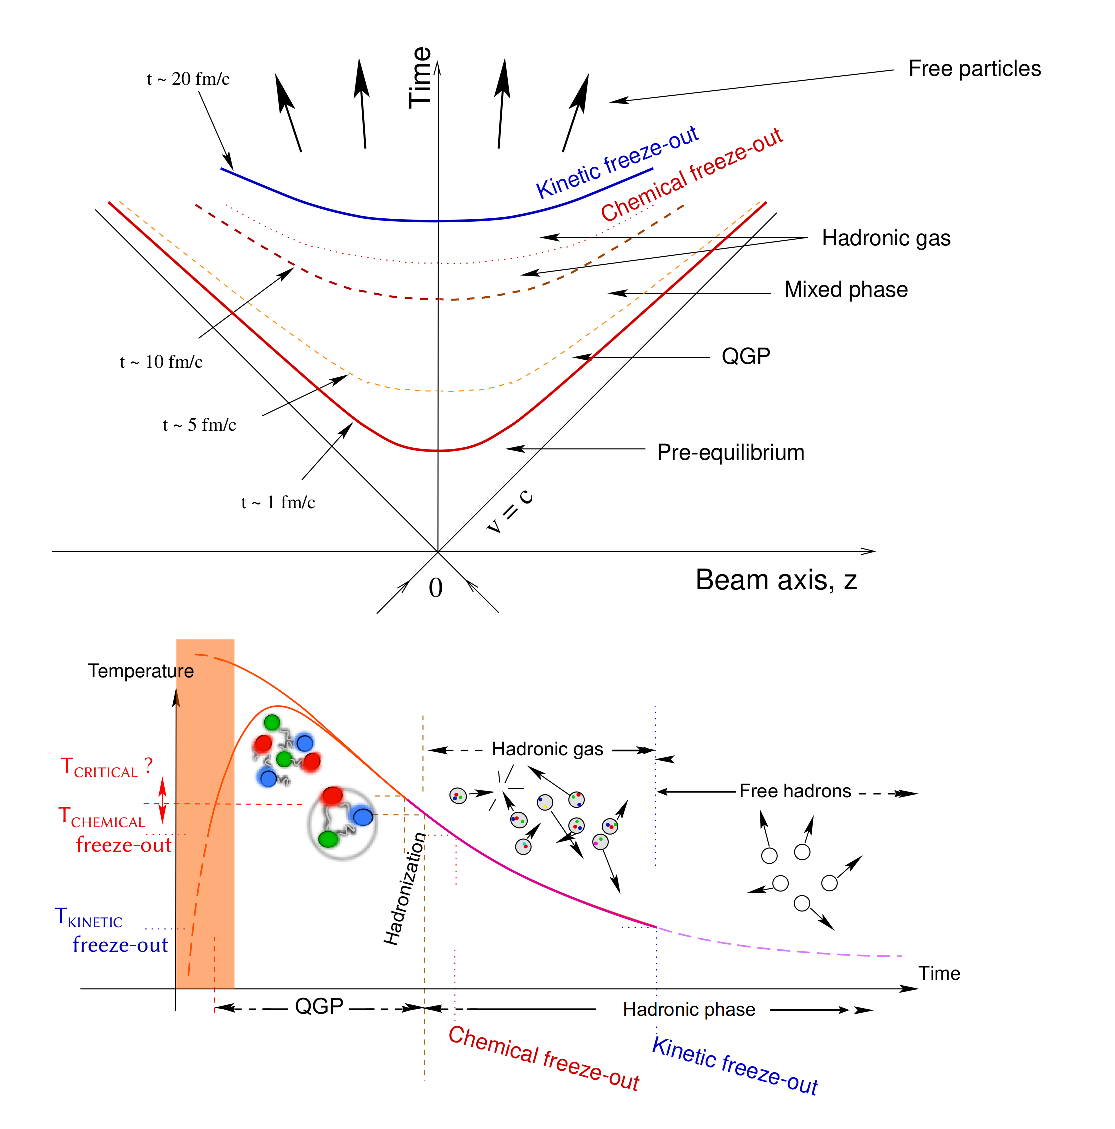
\includegraphics[width=\textwidth]{Figs/Chapter2/Schema-BjorkenScenario.eps}
	\caption{The two views of the Bjorken scenario for ultra-relativistic heavy-ion collisions. Top panel: space-time evolution. Bottom panel: temperature-time evolution. Figure taken from \cite{maireTwoViewsBjorken2011}.}
	\label{fig:QGPEvol}
\end{figure}

The two extremely boosted nuclei approach each other and collide head-on\footnote{Note that this is not necessarily the case, the two nuclei can be slightly shifted. The \textit{impact parameter} quantifies the offset usually in \fm, or alternatively in percentage. In the latter case, we talk about \textit{centrality}. Both parameters are accessible by making use of a \textit{Glauber model}, that provides a semi-classical picture of a nucleus-nucleus collision as a function of the average number of nucleons and nucleon participants in the collision.}. At the same time, the clock associated to the centre-of-mass frame starts to run and indicates 0 \fmC. 

The partons of each nuclei start interacting via either hard-processes -- that involve large momentum transfers and lead to the creation of high momentum partons or massive quarks such as the charm, bottom or even top quarks -- or soft-processes, characterised by small momentum transfer and representing most of the interactions in the initial stage of the collision. As the number of parton-parton interaction increases, the energy density of the system builds up enabling the creation of quarks and gluons out of the vacuum. Rapidly, a dense region of matter (dubbed "fireball") is formed, where partons are strongly coupled but not yet thermalised. This is the pre-equilibrium phase.

Here, the emphasis is on coloured particles, but other kind particles can be produced in the fireball, namely the leptons and photons. Because i) they carry no colour charge and ii) the typical interaction time of the weak ($\approx 10^{-10} \sec$) and electromagnetic forces ($\approx 10^{-16} \sec$) is too short compared to the timescale of a heavy-ion collision ($\approx 10^{-23} \sec$), they will simply escape the medium unaffected.

%\footnote{Here, the emphasis is on coloured particles, but other kind particles can materialise out of the vacuum, namely the leptons. Because i) they carry no colour charge and ii) the typical interaction time of the weak ($\approx 10^{-10} \sec$) and electromagnetic forces ($\approx 10^{-16} \sec$) is too short compared to the timescale of a heavy-ion collision ($\approx 10^{-23} \sec$), they will simply escape the collision environment.}


If the energy density is high enough (typically around 1 \gev/\fm$^{3}$), the initially produced matter undergoes, first, a phase transition towards the restoration of the chiral symmetry and, if possible, then towards the QGP. Due to multiple interaction between the medium constitutents, the energy gets distributed evenly among them leading the system to a thermal equilibrium around 1 \fmC ($\approx 10^{-23} \sec$) after the collision\footnote{Note that this is not a mandatory step for the QGP formation.}. 

Once the QGP is formed, it experiences two expansions. Driven by the non-uniform geometrical energy distribution in the initial stage of the collision, a pressure gradient appears in the QGP, which results in a radial expansion of the system. Furthermore, the boost of the two incident nuclei causes the plasma of quarks and gluons to inflate in the longitudinal directions. Since the energy deposited initially in the system is fixed and its spatial size keeps extending, the energy density decreases and inevitably, the fireball cools down.\\

At some point, most of the parts of the system goes below the critical temperature, the deconfined partons start to recombine into hadrons. The QGP evaporates into a gas of hadrons. Note, that because the chiral transition -- in this case, from a restored symmetry to a broken one -- occurs below $T_{c}$, the mesons and baryons formed during this hadronisation process only carry the bare mass of their constituents. At least, until the system further cools down and undergoes a phase transition towards a breaking of the chiral symmetry, as explained in the \Sec\ref{subsubsec:chiralsymmetrybreaking}.

The energy density within the hadron gas remains significant, sufficiently to allow for inelastic collisions. Consequently, the chemical composition in terms of particle species is in constant evolution. Around 10 \fmC, as the energy density decreases, inelastic interactions become less and less frequent. They become impossible when the gas reaches the \textit{chemical freeze-out} temperature. The particle composition is now fixed but hadrons can still interact elastically.\\

Although, the hadron content should be fixed, some resonances can still regenerate via pseudo-elastic scattering. This is, for example, the case of the \rmKstarZero that can be recreated through \rmPiPM-\Kminplus interaction. On the other hand, elastic scatterings modify the momentum of one of its decay products. In such a case, the measured yield would decrease.  

At 20 \fmC, the hadron gas fades into free hadrons. The momenta of the hadrons are now fixed. This is the \textit{kinetic freeze-out}. These particles will fly towards the detectors and, for some of them, decay via weak or electromagnetic interactions. Either the particles originate directly from the collision or are decay products, once they have reached the detector, they will be detected and reconstructed, giving rise to an event such as the one displayed in the \fig\ref{fig:ALICEEventDisplay}.

\begin{figure}[h]
	\centering
	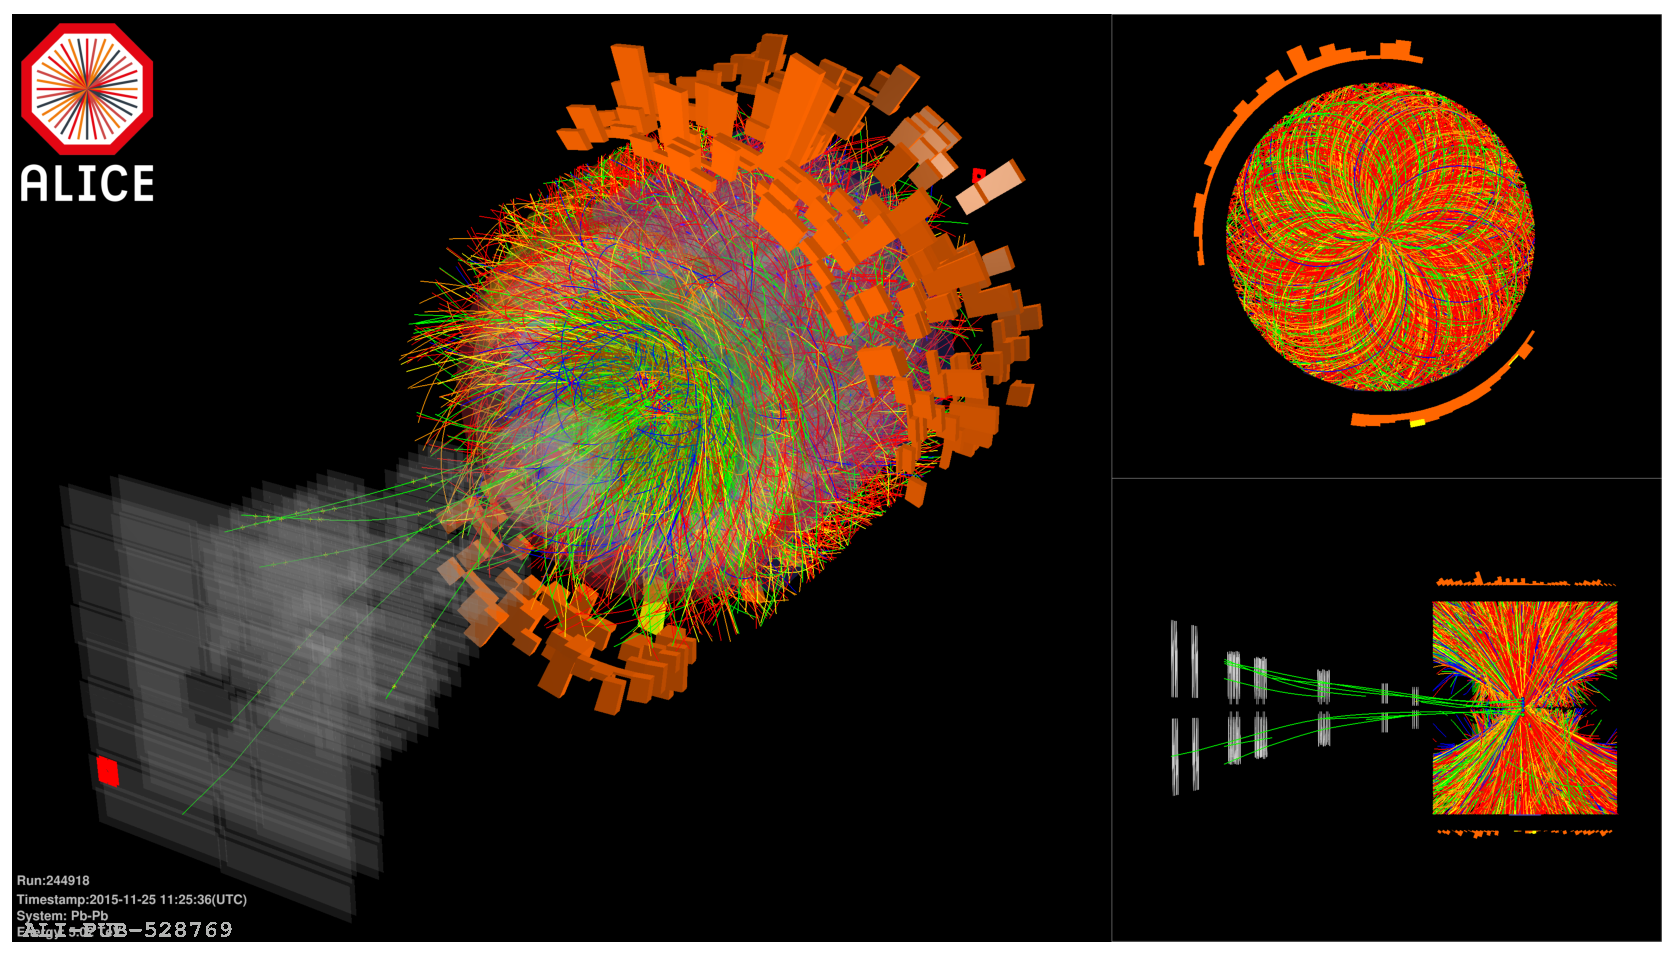
\includegraphics[width=\textwidth]{Figs/Chapter2/ALICE_EventDisplay.eps}
	\caption{Event display of the particles reconstructed with the ALICE detector and created in a Pb-Pb collision at \sqrtSnn = 5.02 \tev in 2015. Figure taken from \cite{alicecollaborationALICEExperimentJourney2022}.}
	\label{fig:ALICEEventDisplay}
\end{figure}

In total, the QGP only exists for about $10^{-22}\sec$, which is currently impossible to reach for the most advanced readout electronics. The study of this state of matter relies on the signatures that are printed in the detectors after the collision. Theoretical models provide predictions of what the QGP footprints look like. Nowadays, it is widely admitted that the following signatures are marks of the QGP.

\begin{itemize}
\item[$\bullet$] \textbf{Collective flow:} The QGP being an almost perfect liquid of constituents with small mean free path, the pressure gradient created by the collision leads to a collective flow, \ie flow of partons, that can be described in the final state by ultra-relativistic hydrodynamic models.  This aspect is addressed, in particular, by performing measurements sensitive to the radial/isotropic and anisotropic flow. The former is characterised by a boost of the low-\pT produced hadrons to higher \pT --- the higher the mass, the higher the boost ---; the latter is studied through a Fourier series decomposition of the azimuthal distribution of the emitted particle density. Moreover, the collective motion of partons can also be observed looking at long-range particle correlation.\\

\item[$\bullet$] \textbf{Direct photons:} Photo-production occurs over the entire duration of the collisions, but it is strongly increased when the system is hot. Therefore, a significant excess of \textit{direct}\footnote{The term \textit{direct} aims at designating only the photons originating from the different stage of the collisions (prompt), and not the ones from hadronic decays (non-prompt).} photons is observed in heavy-ion collisions, suggesting that a QGP has been formed there. Moreover, since they leave the medium unaffected, they carry informations on its properties. In particular, the low-\pT photons are essentially produced out of the plasma heat, hence they are designated as \textit{thermal photons}. Accounting for the blue-shift induced by radial expansion of the system (Doppler effect), the measurement of their yield provides an effective temperature of $304 \pm 41$ \mev in the most central Pb-Pb collisions \cite{alicecollaborationALICEExperimentJourney2022}.\\

\item[$\bullet$] \textbf{Jet quenching:} The high-\pT or massive partons are produced in the early stage of the collision. As they interact with other soft partons of the QGP, a part of their energy is transferred to the medium, resulting in energy loss effects. They are of two kinds: collisional, which consists in elastic scattering \textit{with} the medium constituents, and radiative that corresponds to an inelastic interaction and results in the emissions of gluons \textit{within} the QGP. In the case of two jets, back-to-back, created close to the phase boundary, one will escape the fireball whereas the other will loose most of its energy in the medium. Thus, if one of the back-to-back jets is missing in the event, this would suggest the existence of a hot and dense medium, as observed in \cite{alicecollaborationSuppressionChargedParticle2011}\\

%However, the emission angle decreases with the number of emitted gluons, and the probability of radiating a gluon at a given angle depends on the parton mass. In particular for heavy quarks, there exists a cone region wherein there can be any gluon emission. This is called the \textit{dead cone effect}. Because of that, jets originating from a $c$ or $b$ quark will mainly loose energy \\
\item[$\bullet$] \textbf{Heavy quarkonia suppression:} The heavy quarks, such as charm or beauty, can fragment and hadronise to form a quarkonia ($c\bar{c}$ or $b\bar{b}$ mesons). Because of the low binding energy of these states, they will start to melt and dissolve within the medium. On the other hand, this suppression can be counter-balanced by a regeneration of the quarkonia state: at the chemical freeze-out, it is possible for a heavy quark to recombine with a heavy anti-quark. Therefore, the quarkonia production is compared to theoretical models, and so far, the results are consistent with the formation of a QGP.\\

\item[$\bullet$] \textbf{Hadron abundancy:} At chemical freeze-out, the hadron gas is supposed to be in thermal and chemical equilibrium. The hadron composition in the hadron can therefore be addressed in a statistical approach using the grand canonical formalism. The \textit{statistical hadronisation model} (SHM) provides a prediction of the mesons and baryons abundancies, as a function of the gas volume and temperature, and the different chemical potentials ($\mu_{B}$ for the baryonic one, $\mu_{S}$ for the strangeness one,...). By fitting the measured yields of various hadron species with the SHM prediction, the chemical freeze-out temperature $T_{\textrm{ch}}$ and volume $V_{\textrm{ch}}$ can be estimated. The values $T_{\textrm{ch}} = 155 \pm 2 \ \mev$ and $V_{\textrm{ch}} = 5924 \pm 543 \ \fm^{3}$ are consistent with lattice QCD calculations. \\
\end{itemize}

About abundancy, the one of strange particles stands out of the other species. It is, in fact, one of the historical key signatures of the QGP and is called the \textit{strangeness enhancement}. 

\subsection{Strangeness enhancement}
\label{subsec:StrangenessEnhanement}

The concept of strangeness enhancement, that consists in the abundant production of strange hadrons in heavy-ion collisions, starts to take shape in the mind of Johann Rafelski in 1980. The original argument is based on the assumption that, in a melted vacuum such as the one that settles in the QGP pre-equilibrium stage, the chiral symmetry restoration results in strange quarks carrying only their bare mass ($m_{s}$), that is at least two times lower than QGP temperature ($2 m_{s} < T_{\textrm{QGP}}$) . Thus, this opens the way to a chemical equilibration/saturation of strangeness. When the fireball cools down, the numerous $s$ and $\bar{s}$ tend to hadronise into strange baryons ($qqs$ or $\bar{q}\bar{q}\bar{s}$,...) rather than mesons ($\bar{q}s$ or $q\bar{s}$).

Back then, gluons were still hypothetical objects. Strangeness production was mainly considered in the annihilation process of light quark pairs $q\bar{q} \rightarrow s \bar{s}$ (\fig\ref{fig:StrangeYields}d). In 1981, J\'ozsef Zim\'anyi and Tam\'as B\'ir\'o estimated that, with this process, the chemical equilibrium of strangeness takes too much time to settle and is reached around eight times the natural lifespan of a QGP fireball. However, Zim\'anyi and B\'ir\'o assumed that there were no gluons and were focused on the physical case of a hadron gas \cite{rafelskiStrangenessEnhancement2008}.

In parallel, it was realised that gluon fusion processes dominates the production rates. Together with Berndt M\"{u}ller, Rafelski shows in 1982 that the chemical equilibration of strangeness is possible within the QGP lifespan thanks to the fusion of gluons created out of the vacuum heat  \cite{rafelskiStrangenessProductionQuarkGluon1982}. The different $gg \rightarrow s\bar{s}$ processes are depicted in \fig\ref{fig:StrangeYields}a,b,c.

%\begin{figure}[h]
%	\centering
%	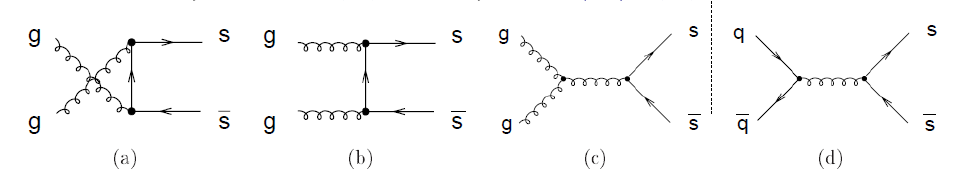
\includegraphics[width=1\textwidth]{Figs/Chapter2/Screenshot_20220620_004959.png}
%	\caption{The lowest-order QCD diagrams for $s\bar{s}$ production. (a)(b)(c) the different gluon fusion processes $gg\rightarrow s\bar{s}$; (d) quark-antiquark annihilation process $q\bar{q} \rightarrow s\bar{s}$. Figure taken from \cite{maireProductionBaryonsMultietranges2011}.}
%	\label{fig:StrangenessEnhancement}
%\end{figure}

\begin{figure}[h]
	\begin{minipage}{0.33\textwidth}
		\subfigure[]{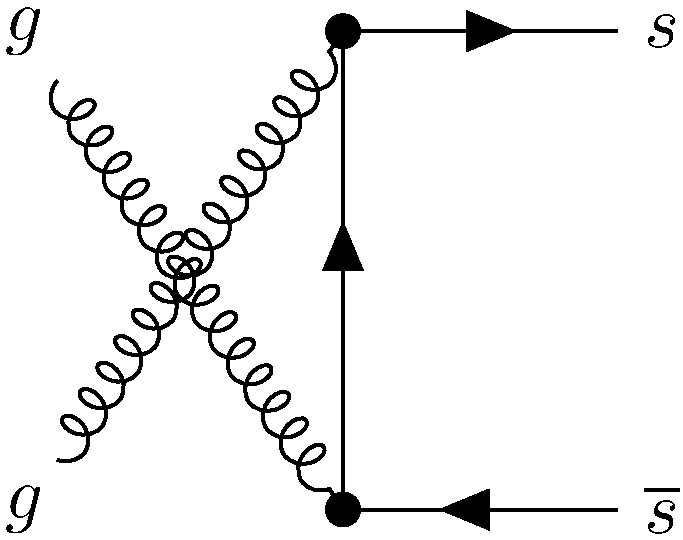
\includegraphics[width=0.75\textwidth]{Figs/Chapter2/g+g_crossed_to_s+sbar.pdf}}
	\end{minipage}%
	\begin{minipage}{0.33\textwidth}
		\subfigure[]{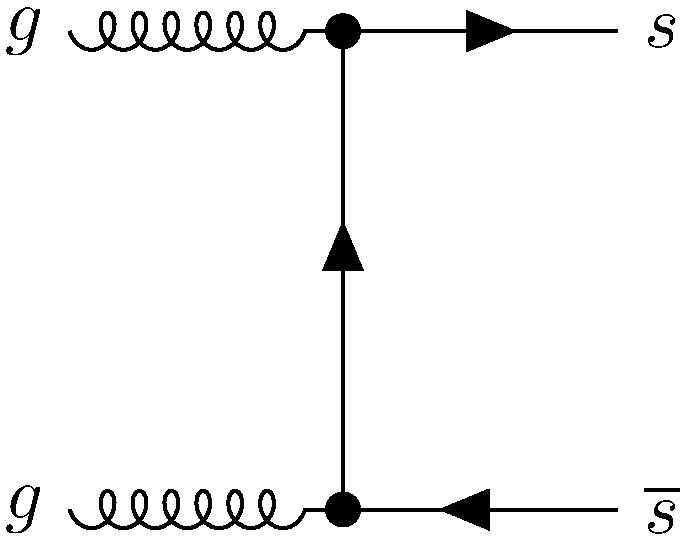
\includegraphics[width=0.75\textwidth]{Figs/Chapter2/g+g_square_to_s+sbar.pdf}}
	\end{minipage}%
	\begin{minipage}{0.33\textwidth}
		\subfigure[]{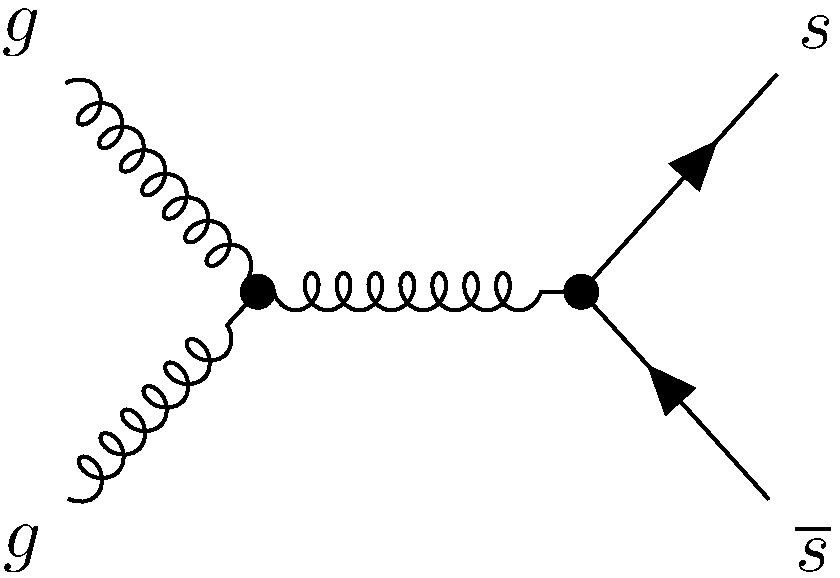
\includegraphics[width=0.90\textwidth]{Figs/Chapter2/g+g_to_gluon_to_s+sbar.pdf}}
	\end{minipage}\par\medskip
	\centering
	\begin{minipage}{0.33\textwidth}
		\subfigure[]{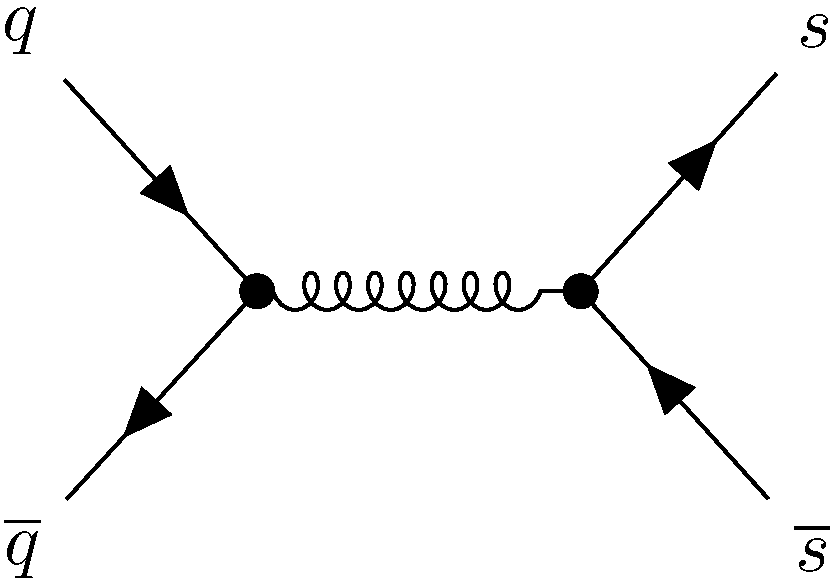
\includegraphics[width=0.90\textwidth]{Figs/Chapter2/q+qbar_to_gluon_to_s+sbar.pdf}}
	\end{minipage}%
	\caption{The lowest-order QCD diagrams for $s\bar{s}$ production. (a)(b)(c) the
	 different gluon fusion processes $gg\rightarrow s\bar{s}$; (d) quark-antiquark annihilation process $q\bar{q} \rightarrow s\bar{s}$. Figure taken from \cite{maireProductionBaryonsMultietranges2011}.}
	\label{fig:StrangenessEnhancement}
\end{figure}



In summary, the strangeness enhancement was proposed by Rafelski and M\"{u}ller in 1982 as a signature of a deconfined quark-gluon matter. They demonstrated that:
\begin{itemize}
\item the QGP begins to be saturated by strange quarks and anti-quarks when the temperature of the plasma reaches the 200 \mev after about $2 \times 10^{-23} \sec$,
\item this saturation is possible because strange quarks can pop in out of the QGP heat ($2 m_{s} < T$) via gluon fusion processes (\fig\ref{fig:StrangenessEnhancement}). These processes are favoured because i) they are more energy/time efficient and ii) the high density of gluons created out of the vacuum,
\item at the hadronisation, the strangeness tends to be distributed on baryons rather than mesons. Consequently, this leads to an increased production of strange particles in the final state of the collision. In fact, the larger the strangeness content, the larger the enhancement of the hadron production.\\
\end{itemize}

Experimentally, the strangeness enhancement manifests itself through an increase of the \textit{relative} yields of strange hadrons in heavy-ion collisions. Now comes two difficulties: so far, only the strangeness enhancement from the formation of a QGP was considered, however a similar phenomenon could occur in a hadron gas\footnote{Strange hadrons could be formed via inelastic collisions between light mesons and baryons. Because of the large dynamical mass of hadrons, the production of strange particles should be suppressed. This reduction gets more pronunced as the hadron mass is high.}. The difference between these two increases in strange particle abundancies resides in the hierarchy between hadrons with different strangeness content \cite{maireProductionBaryonsMultietranges2011}:

\begin{align}
\rmOmega(sss)\ /\ \rmXi(dss) _{\textrm{QGP}} \quad &\approx \quad \rmXi(dss)\ /\ \rmLambda(uds) _{\textrm{QGP}}\\
\rmOmega(sss)\ /\ \rmXi(dss) _{\textrm{Hadron Gas}} \quad &\ll \quad \rmXi(dss)\ /\ \rmLambda(uds) _{\textrm{Hadron Gas}}
\end{align}

\begin{align}
\rmOmega(sss)\ /\ \rmXi(dss) _{\textrm{QGP}} \quad &> \quad \rmOmega(sss)\ /\ \rmXi(dss) _{\textrm{Hadron Gas}}\\
\rmXi(dss)\ /\ \rmLambda(uds) _{\textrm{QGP}} \quad &> \quad \rmXi(dss)\ /\ \rmLambda(uds) _{\textrm{Hadron Gas}}
\end{align}


Another issue arises from the definition of \textit{relative} yields. In other words, this comes down to asking what normalisation to use? There are different possibilities, depending on the physics target. Most of the time, the yields of strange hadrons in heavy-ion collisions are compared to the ones in pp collisions. This is relevant in order to discriminate the strangeness enhancement originating from the QGP (heavy-ion collisions) from the one occuring in a hadron gas (as in pp collisions, assuming that there are enough interactions between the different produced hadrons). Alternatively, one could also look at the "continuous" evolution of the yields as a function of the collision system. In such a case, the relative yields correspond to the ratio of production rate between the particle of interest and the lighest known hadron, namely the \rmPi. Finally, the focus can also be on the difference of yields between hadrons with the same strangeness content but different mass, typically the yields ratio between a resonant and a non-resonant hadronic state. This could provide some information on the influence of the hadronic phase.\\

\begin{figure}[h]
	\centering
	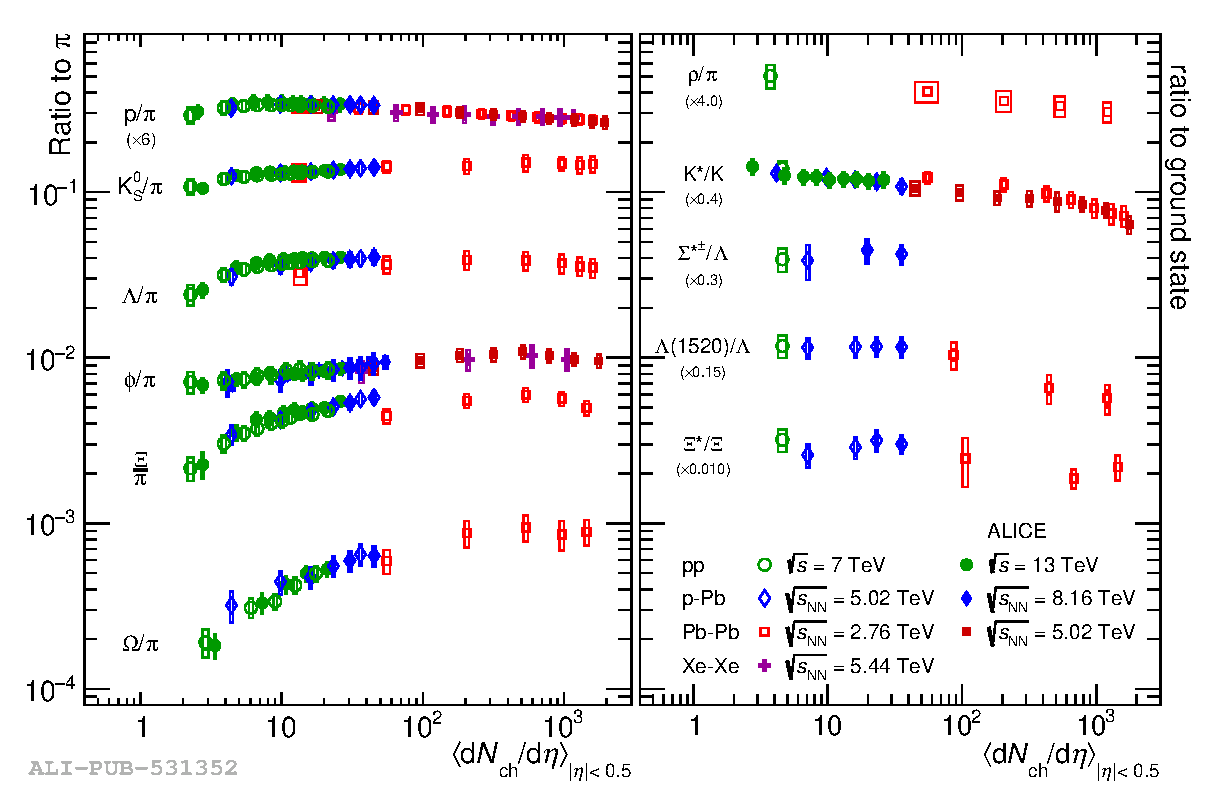
\includegraphics[width=1\textwidth]{Figs/Chapter2/fig3.2a.eps}
	\caption{(Left panel) Relative yields of strange hadrons with respect to the pions and (right panel) yield ratios between resonant and ground state hadrons as a function of the average charged particle multiplicities at midrapidity. Results from different collision systems are presented: pp at \sqrtS = 7 and 13 \tev; p-Pb at \sqrtSnn = 5.02 and 8.16 \tev; Pb-Pb at \sqrtSnn = 2.76 and 5.02 \tev; Xe-Xe at \sqrtSnn = 5.44 \tev. The left panel considers the following strange hadrons: \rmKzero ($\bar{d}s$), \rmLambda ($uds$), \rmPhi ($s\bar{s}$), \rmXi ($dss$) and \rmOmega ($sss$). The error bars corresponds to the statistical uncertainty, whereas the boxes show the total systematic uncertainty. Figure taken from \cite{alicecollaborationALICEExperimentJourney2022}.}
	\label{fig:StrangeYields}
\end{figure}

The \fig\ref{fig:StrangeYields} presents, on the left, the measurement of relative yields of strange hadrons with respect to the pions a function of the average charged multiplicity of the collision, and on the right, the yield ratios between resonant and non-resonant states are displayed. The lowest multiplicities correspond to pp collisions, and as it increases, we move on towards more and more central heavy-ion collisions.

The left panel of \fig\ref{fig:StrangeYields} shows that the yield of strange hadrons increases in Pb-Pb and Xe-Xe collisions with respect to pp and p-Pb collisions, and the enhancement factor gets bigger with the strangeness content. This is compatible with the strangeness enhancement picture and confirms the existence of a deconfined quark-gluon matter. Notice that the ratios do not change with the centre-of-mass energy, suggesting that the initial stage of the collision does not play an important role in the strangeness enhancement (at least, at the LHC energies).

On the right panel, the yield ratios between resonant and non-resonant hadronic states seems to decrease when going from elementary collision systems (pp and p-Pb) to the heavy-ion ones. This trend indicates that the temperature of the hadron gas after the QGP is sufficiently high to suppress the resonance yields by elastic rescattering of the decay products.

%\begin{figure}
%\unitlength = 1mm
%\centering
%\subfigure[]{
%	\begin{fmffile}{ggxss}
%	\begin{fmfgraph*}(40,25)
%	\fmfleft{i1,i2}
%	\fmfright{o1,o2}
%	\fmflabel{$g$}{i1}
%	\fmflabel{$g$}{i2}
%%	\fmflabel{$s$}{o1}
%%	\fmflabel{$\bar{s}$}{o2}
% 	\fmf{fermion}{o1,v1}
% 	\fmf{fermion,tension=0}{v1,v2}
% 	\fmf{fermion}{v2,o2}
% 	\fmffreeze
%	\fmf{gluon}{i1,v1}
%	\fmf{gluon,rubout}{i2,v2}
%%    \fmf{fermion}{i1,v1,v2,o1}
%%	\fmf{fermion}{o2,v4,v3,i2}
%%	\fmf{photon,tension=0}{v1,v3}
%%	\fmf{photon,tension=0}{v2,v4}
%	\end{fmfgraph*}
%	\end{fmffile}
%}
%\subfigure[]{
%	\begin{fmffile}{gghss}
%	\begin{fmfgraph*}(35,25)
%	\fmfleft{i1,i2}
%	\fmfright{o1}
%	\fmflabel{$g$}{i1}
%	\fmflabel{$g$}{i2}
%	\fmflabel{$g$}{o1}
%	\fmf{gluon}{i1,v1}
%	\fmf{gluon}{i2,v1}
%	\fmf{gluon}{v1,o1}
%	\fmfv{lab=$g_s$,lab.dist=0.15w}{v1}
%	\fmfdot{v1}
%	\end{fmfgraph*}
%	\end{fmffile}
%}
%\subfigure[]{
%	\begin{fmffile}{ggss}
%	\begin{fmfgraph*}(40,25)
%	\fmfleft{i1,i2}
%	\fmfright{o1,o2}
%	\fmflabel{$g$}{i1}
%	\fmflabel{$g$}{i2}
%	\fmflabel{$s$}{o1}
%	\fmflabel{$\bar{s}$}{o2}
%	\fmf{gluon}{i1,v1}
%	\fmf{gluon}{v1,i2}
%	\fmf{fermion}{v2,o1}
%	\fmf{fermion}{o2,v2}
%	\fmf{gluon}{v1,v2}
%	\fmfdot{v1}
%	\fmfdot{v2}
%	\end{fmfgraph*}
%	\end{fmffile}
%}
%\subfigure[]{
%	\begin{fmffile}{qqss}
%	\begin{fmfgraph*}(40,25)
%	\fmfleft{i1,i2}
%	\fmfright{o1,o2}
%	\fmflabel{$q$}{i1}
%	\fmflabel{$\bar{q}$}{i2}
%	\fmflabel{$s$}{o1}
%	\fmflabel{$\bar{s}$}{o2}
%	\fmf{fermion}{i1,v1}
%	\fmf{fermion}{v1,i2}
%	\fmf{fermion}{v2,o1}
%	\fmf{fermion}{o2,v2}
%	\fmf{gluon}{v1,v2}
%	\fmfdot{v1}
%	\fmfdot{v2}
%	\end{fmfgraph*}
%	\end{fmffile}
%}
%\caption{Using \texttt{test}}
%\end{figure}

\subsection{Comparison with elementary systems}
\label{subsec:ComparisonPP}

Throughout this section, it was suggested that the formation of the QGP is exclusive to heavy-ion collisions, and it is not expected in more elementary systems -- such as pp and p-Pb collisions -- because the size of the colliding system is \textit{a priori} too small. Looking more attentively at the \fig\ref{fig:StrangeYields}, one notices that relative yields of strange hadrons increases smoothly from low to high multiplicity pp and p-Pb collisions. In other words, this means that strangeness enhancement seems to be present as well in small systems.

In fact, the aforementionned QGP manifestations, the heavy quarkonia suppression \cite{adamCentralityDependence2S2016}, the strangeness enhancement \cite{alicecollaborationALICEExperimentJourney2022}, the collective flow \cite{schotterQCDLHC2022} have been observed in both heavy-ion collisions and small systems, suggesting the presence of a common collective behaviour. Some signatures are missing though; for example, there are so far no indication of jet quenching nor thermal photons in small systems. 

As a consequence, the classical picture of a heavy-ion collision, forming a hot and dense matter where quarks and gluons are deconfined, needs to be revised. At least, the elementary colliding systems can no longer be considered as a valid reference point, for sufficiently high energies such as the LHC ones. This point will be further addressed in more details in \chap\ref{chap:CorrelatedAnalysis}.



 % Data sets
\newpage
%//------ Section 02 -------------------------------------------------------------------------------------------------
\chapter{A Large Ion Collider Experiment: a journey through QCD}
\label{sec:Section02}
%//-----------------------------------------------------------------------//

Located the border between France and Switzerland, the CERN is like a tiny country with its own culture, its own language (essentially composed of acronyms). % The ALICE experiment
\newpage
%//------ Section 04 -------------------------------------------------------------------------------------------------
\chapter{Identification of V0 particles and cascades}
\label{chap:V0CascReconstruction}
%//-----------------------------------------------------------------------//

The \chap\ref{chap:ParticlePhysics} and \ref{chap:ALICE} have set the scene, it is time for the main actors to come onto stage, that are the (multi-)strange baryons or more precisely, the \textit{hyperons}. These consist of any baryon containing at least one strange quark, but no heavier quarks such as charm, bottom (or top...). By describing their identification and the physics interests surrounding their reconstruction, this short chapter lays the foundations for the analyses performed throughout this thesis.\\

The first section, \Sec\ref{sec:StrangenessFeatures}, underlines the appealing features of strangeness and, particularly, (multi-)strange particles. The hyperons of interest in the present analyses are specified in the following section, \Sec\ref{sec:HyperonId}, as well as the motivations for this choice. This part also presents the principles for multi-strange baryon identification via topological reconstruction. Finally, in connection with \chap\ref{chap:ALICE}, this short chapter closes on what makes ALICE a unique experiment for studying strange hadrons.


\section{The appealing features of strangeness}
\label{sec:StrangenessFeatures}

\subsection{The strange quark with respect to the other flavours}

Similarly as for the charm, bottom and top quarks, there is no strangeness among the \emph{valence} quarks of the nucleons from the collision beams. At first sight, these only consist in up and down quarks.
Admittedly, other quark flavours can still be found inside the sea of quarks and gluons,
in amounts that even rise while the momentum fraction carried by such initial partons gets smaller and smaller. However, those almost always do not take part in the collision processes\footnote{Gluon fusion processes dominate the collision picture from the very low momentum fraction~$x_{\rm B}$ up to $x_{\rm B} \approx 0.05$, that is, at mid-rapidity, to any outcome object originating from processes with energy transfer up to $Q = \sqrtS \cdot x_{\rm B} = 13~\tev \cdot 0.05 = 650~\gev$, meaning up to high energy scale.}. From this, there arises an interesting and straightforward aspect of strangeness: the vast majority of the strange quarks observed in the final state hadrons must have been produced in the processes that have occurred during the collision.

Another property regards the mass of the strange quark. One way of classifying quarks is based on whether they preserve (at least, approximatively) or break the chiral symmetry (\Sec\ref{subsubsec:chiralsymmetrybreaking}): the up and down quarks belongs to the first kind and makes part of the light flavour sector. Those breaking the chiral symmetry -- the charm, bottom and top quarks -- constitute the heavy flavour sector. For comparison, the \emph{bare} mass of the up quark sits at $2.16_{-0.26}^{+0.49}$ \mmass, the down quark at $4.67_{-0.17}^{+0.48}$ \mmass. In contrast, the one of the charm, bottom and top quarks lie around $1.27 \pm 0.02$ \gmass, $4.18_{-0.02}^{+0.03}$ \gmass and $172.69 \pm 0.30$ \gmass respectively~\cite{particledatagroupReviewParticlePhysics2022}. From this perspective, the strange quark with its bare mass of $93.4_{-3.4}^{+8.6}$ \mmass holds a unique position: its lightweight makes it relatively inexpensive (in terms of energy) to produce; being still much heavier than the up and down quarks (by one order of magnitude), this also qualifies it as non-ordinary matter. Thus viewed as both light and heavy, the strange quark gives access to an \emph{abundant} source of \emph{non-ordinary} matter and information about the collision dynamics.


\subsection{The specificity of strange hadrons}
\label{subsec:SpecStrangeHadrons}

Most of strange hadrons decays into charged particles in their dominant channel. In addition, they also have a relatively long lifetime, allowing them to fly over several centimeters before the decay. From these two elements stem the distinctive decay topology of strange particles known as V0 or cascade (\Sec\ref{subsec:V0CascDecays}), that can be used in their reconstruction by associating the different daughter tracks to reform the decay vertex (topological reconstruction, detailed later in \Sec\ref{subsec:TopoReco}) \cite{speltzCaracterisationEtatDense2006}. This characteristic turns out to be particularly interesting as the latter provides a robust identification of strange hadrons over a wide momentum range, from low to high \pT.

Consequently, this offers the possibility for a continuous study of strange hadrons over different production regimes, involving soft, intermediate and hard processes such as multi-parton interactions, quark coalescence and jet fragmentation respectively. For that reason, strange particles represents prime-choice probes to investigate and thus improve our understanding on the evolution of the hadronisation mechanisms\footnote{To be exact, it is not the hadronisation mechanisms that evolves with the transverse momentum but rather their relative weight. For instance, quark coalescence happens mostly at intermediate \pT but it can still occur at high momentum, although with a different probability.} with momentum.

\section{The multi-strange baryon identification}
\label{sec:HyperonId}

Among all the strange hadrons, this work focuses on the strangest baryons, containing two or three strange quarks, the so-called multi-strange baryons. Excluding the associated resonances, this leaves five particles: three containing two strange quarks -- the \rmXiZero\ ($uss$), \rmXiM ($dss$) and \rmAxiP ($\bar{d}\bar{s}\bar{s}$) -- and two triple-strange hadrons namely the \rmOmegaM ($sss$) and \rmAomegaP ($\bar{s}\bar{s}\bar{s}$).

\begin{table}[t]
    \centering
    \begin{tabular}{b{2cm}@{\hspace{0.25cm}} b{2cm}@{\hspace{0.5cm}} b{2cm}@{\hspace{0.25cm}} b{2cm}@{\hspace{0.25cm}} b{3cm}@{\hspace{0.5cm}} b{1.5cm}@{\hspace{0.25cm}}}
    \noalign{\smallskip}\hline\noalign{\smallskip}
	Particle & Strangeness & Mass (\mmass) & Lifetime (\cm) & Dominant decay channel & B.R. \\
    \noalign{\smallskip}\hline \noalign{\smallskip}
    
    \rmLambda [$u d s$] & $+1$ &1115.683 & 7.89 & \proton [$uud$] \piMinus\ [$\bar{u} d$] & \textsc{63.9 \%} \\
    \rmAlambda [$\bar{u}\bar{d}\bar{s}$] & $-1$ & 1115.683 & 7.89 & \pbar [$\bar{u} \bar{u} \bar{d}$] \piPlus\ [$u \bar{d}$] & \textsc{63.9 \%} \\
    
    \noalign{\smallskip}\hline \noalign{\smallskip}    
    
    \rmXiZero\ [$uss$] & $+2$ & 1314.86 & 8.71 & \rmLambda [$u d s$] \piZero\ [$u\bar{u}$] & \textsc{99.6 \%}\\
    
    \noalign{\smallskip}\hline \noalign{\smallskip}    
    
    \rmXiM [$dss$] & $+2$ & 1321.71 & 4.91 & \rmLambda [$u d s$] \piMinus\ [$\bar{u} d$] & \textsc{99.9 \%}\\
	\rmAxiP [$\bar{d}\bar{s}\bar{s}$] & $-2$ & 1321.71 & 4.91 & \rmAlambda [$\bar{u}\bar{d}\bar{s}$] \piPlus\ [$u\bar{d}$] & \textsc{99.9 \%}\\
	
    \noalign{\smallskip}\hline \noalign{\smallskip}
    
	\rmOmegaM [$sss$] & $+3$ & 1672.45 & 2.461 & \rmLambda [$u d s$] \Kminus\ [$\bar{u} s$] & \textsc{67.8 \%}\\
	\rmAomegaP [$\bar{s}\bar{s}\bar{s}$] & $-3$ & 1672.45 & 2.461 & \rmAlambda [$\bar{u}\bar{d}\bar{s}$] \Kplus\ [$u\bar{s}$] & \textsc{67.8 \%}\\
    
    \noalign{\smallskip}\hline\noalign{\smallskip}
    \end{tabular}
    \caption{Main characteristics of the \rmLambda and the (charged) multi-strange baryons: quark content, strangeness, tabulated mass and lifetime (\cTau), dominant decay channel with the associated branching ratio (B.R.) \cite{particledatagroupReviewParticlePhysics2022}.}\label{tab:V0CascDecay}
\end{table}

\Tab\ref{tab:V0CascDecay} shows some characteristics of these five baryons, including their dominant decay channel, as well as the mono-strange baryon \rmLambda since it appears in all decay channels. Unlike the \rmXiZero, the four charged multi-strange baryons share a common feature and a particularly appealing one: in their dominant decay channel, they follow a cascade decay topology as 
detailed in the next section, \Sec\ref{subsec:V0CascDecays}. For that reason, the present work concentrates on the study of \emph{charged} multi-strange baryons, \ie putting aside the \rmXiZero\ species.\\


From now on, the following notations will be used. The \rmXiPM (\rmOmegaPM) notation refers to \rmXiM \emph{or} \rmAxiP (\rmOmegaM \emph{or} \rmAomegaP). Conversely, \rmXi (\rmOmega) means \rmXiM \emph{and} \rmAxiP (\rmOmegaM \emph{and} \rmAomegaP). The same goes for other particles. Moreover, unless indicated otherwise, the term multi-strange baryon now designates only the \rmXiM, \rmAxiP, \rmOmegaM or \rmAomegaP.


\subsection{The V0 and cascade decays}
\label{subsec:V0CascDecays}


\Fig\ref{fig:CascadeDecay} depicts the full cascade decay chain of \rmXi and \rmOmega. After flying over a few centimeters, the multi-strange baryon decays weakly into a charged pion (or kaon for the \rmOmega) and a \rmLambda. The latter being electrically neutral, only the charged meson deposits energy in the different sensitive layers and thus can be detected at this stage; the meson plays the role of a \textit{bachelor} particle. 

\begin{figure}[t]
	\centering
	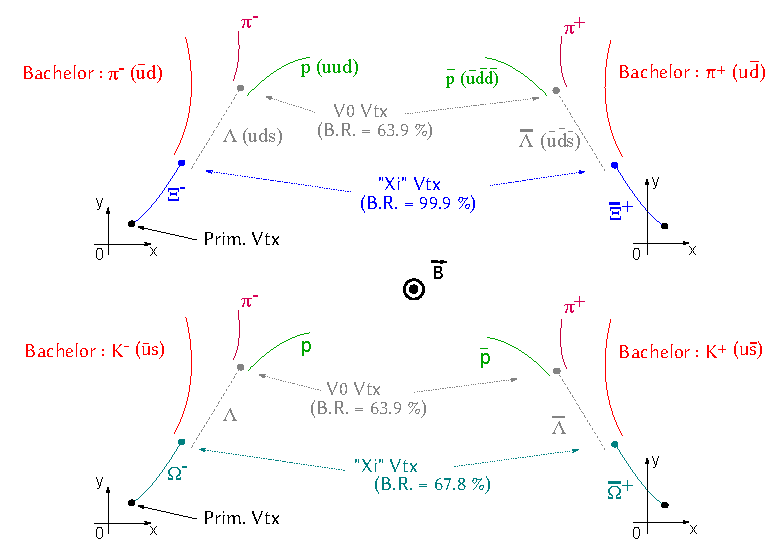
\includegraphics[width=1\textwidth]{Figs/Chapter4/Schema-4TypesDeCascade.eps}
	\caption{Depiction of the full cascade decay chain of the \rmXiM (top left), \rmAxiP (top right), \rmOmegaM (bottom left) and \rmAomegaP (bottom right). Figure taken from \cite{maireFourTypesCascade2011}.}
	\label{fig:CascadeDecay}
\end{figure}

The two decay products continue to travel through the detector, until the baryon daughter decays\footnote{The bachelor daughter being either a \rmPiPlusMinus or \Kplusmin, in most cases it does not decay in the detector due to their long lifetime ($\cTau_{\pi} = 7.8045$ \m and $\cTau_{\rm K} = 3.711$ \m). For those that actually decays in the detector, they are characterised by a \textit{kink} topology due to their decay into a charged particle and a neutral particle.} in  63.9\% of the cases via weak interaction into two oppositely charged particles: a proton and a pion. Depending on their electric charge, one is called the \textit{positive} particle and the other the \textit{negative} particle. This decay topology is known as V0\footnote{The term \say{V0} comes from the V-shape decay topology formed by the two oppositely charged decay daughters.}. Furthermore, the term \say{cascade} refers to the two-steps decay process undergone by the multi-strange baryons. Hence, in the following, the usage of the term \textit{cascade} may be used to mention either the \rmXi or \rmOmega, and similarly the term \textit{V0} for the \rmLambda.

Note that the four cascades on \fig\ref{fig:CascadeDecay} differ only in the nature of the particles involved. On one hand, from the left to right side, the particles are swapped to anti-particles. On the other hand, the larger strangeness content of the \rmOmega imposes the presence of a bachelor particle containing a strange quark (kaon) while, in the \rmXi case, it consists in a light unflavoured meson (pion).

It should also be mentioned that although the \rmXiPM decays into this channel quasi-systematically (99.9\%), this is only the case for 67.8\% of the \rmOmegaPM.\\

\begin{figure}[t]
	\centering
	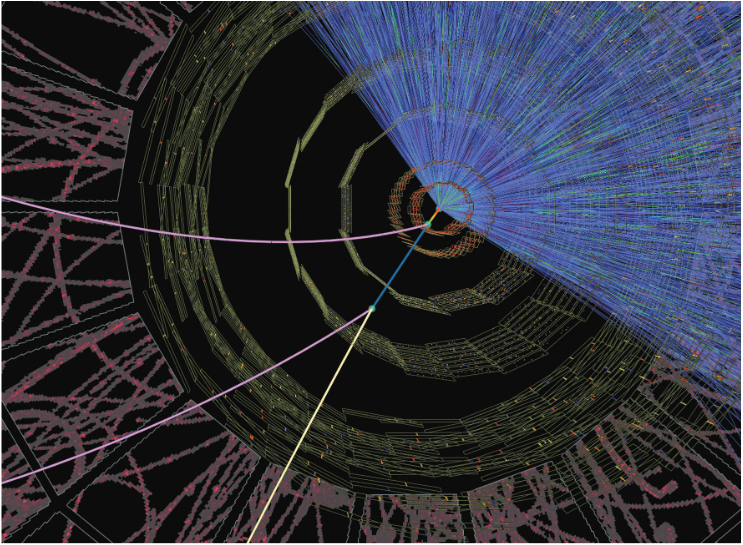
\includegraphics[width=1\textwidth]{Figs/Chapter4/XiEventDisplay.png}
	\caption{Event display of a simulated Pb-Pb collision in the ALICE detector, with a close-up on the ITS. The top part illustrates the typical density of tracks in such environment. The bottom part highlights the cascade decay of a \rmXiM. Figure taken from \cite{alicecollaborationALICEPhysicsPerformance2006}.}
	\label{fig:CascadeDecaySimu}
\end{figure}

\Fig\ref{fig:CascadeDecaySimu} shows the cascade decay of a \rmXiM within the ALICE detector. To make it more apparent, the surrounding tracks have been removed in the bottom left part. The \rmXiPM or \rmOmegaPM being electrically charged, they may loose energy in the detectors and can \textit{a priori} be detected as any other charged particle. Although they can fly over relatively long distance compared to the vast majority of unstable particles, their \cTau remain too short to \textit{systematically} reach the innermost detectors at about 3.9 \cm and 7.6 \cm (to be compared to $\cTau_{\Xi}$ = 4.91 \cm and $\cTau_{\Omega}$ = 2.461 \cm)\footnote{Note that the detection and tracking of these two multi-strange baryons become more likely with the upgraded version of the ITS in the LHC Run-3; the innermost silicon pixel detectors being positioned at a radius of 2.2 \cm and 3.9 \cm in the LHC, the \rmXi and \rmOmega have significantly more chances to leave hits in this detection layers, and therefore to be detected \cite{chinellatoCharmMulticharmBaryon2022}.}. Moreover, the \rmLambda being a neutral particle, hence it cannot deposit energy in the sensitive layers. In summary, only the bachelor, the positive and negative particles can be detected\footnote{Due to their long lifetime, the detection of the \rmPiPlusMinus, \Kplusmin, \proton and \pbar relies on the reconstruction and identification of their associated tracks in the ITS and TPC.}. Therefore, it follows that the V0 and cascade have to be identified indirectly via their decay topology.

The top right part of \fig\ref{fig:CascadeDecaySimu} puts into perspective the difficulty of the reconstructing such a cascade topology in an event with a large combinatorial background. While the bottom part of the figure shows clearly the \rmXiM decay chain, it actually is immersed in a dense environment. In order to identify the multi-strange baryons in the event, the strategy followed in the present work consists in using topological reconstruction.

\subsection{The principles of the topological reconstruction}
\label{subsec:TopoReco}

The cascade reconstruction is achieved by combining three tracks in the event. The association of two tracks of opposite curvature signs allows to build a \rmLambda (or \rmAlambda) candidate, that may in turn be associated to another track (the bachelor) to form a cascade candidate. In a pp collision, the charged particle density\footnote{per unit of pseudo-rapidity.} can vary from a few particles up to fifty, and more than a thousands in the most central heavy-ion collisions. The mere association of three tracks leads inexorably to the formation of erroneous candidates, thus constituting a source of \textit{combinatorial} background. In order to suppress the latter, geometric selections -- aimed at singling out the candidates spatially compatible with the expected decay topology -- are introduced; this is the general principle behind topological reconstruction.

\subsubsection{Formation of the V0 candidates}
\label{subsubsec:V0Formation}

The reconstruction starts with the formation a V0 candidate. The first step consists in identifying \textit{secondary} tracks, that do not originate from the interaction point. They are tagged as such, if the distance of closest approach (DCA) between the considered track and the primary vertex exceeds a critical value\footnote{While one expects for a primary track to have a DCA to the primary vertex equal (or close) to zero, this is the opposite for a secondary track: since it does not originate from the collision point, its DCA to the interaction vertex must necessarily be different from zero.} (\fig\ref{fig:TopologicalRec}, V0.a). 

The second step aims at forming pairs of secondary tracks of opposite charge, \ie characterised by different curvatures; by imposing that the DCA between the two tracks is small, only the pairs originating potentially from the same decay point are retained. The secondary vertex is then positioned on the segment defined by the previous DCA, weighted by the quality of the tracks (\fig\ref{fig:TopologicalRec}, V0.b).

\afterpage{
\begin{figure}[H]
	\centering
	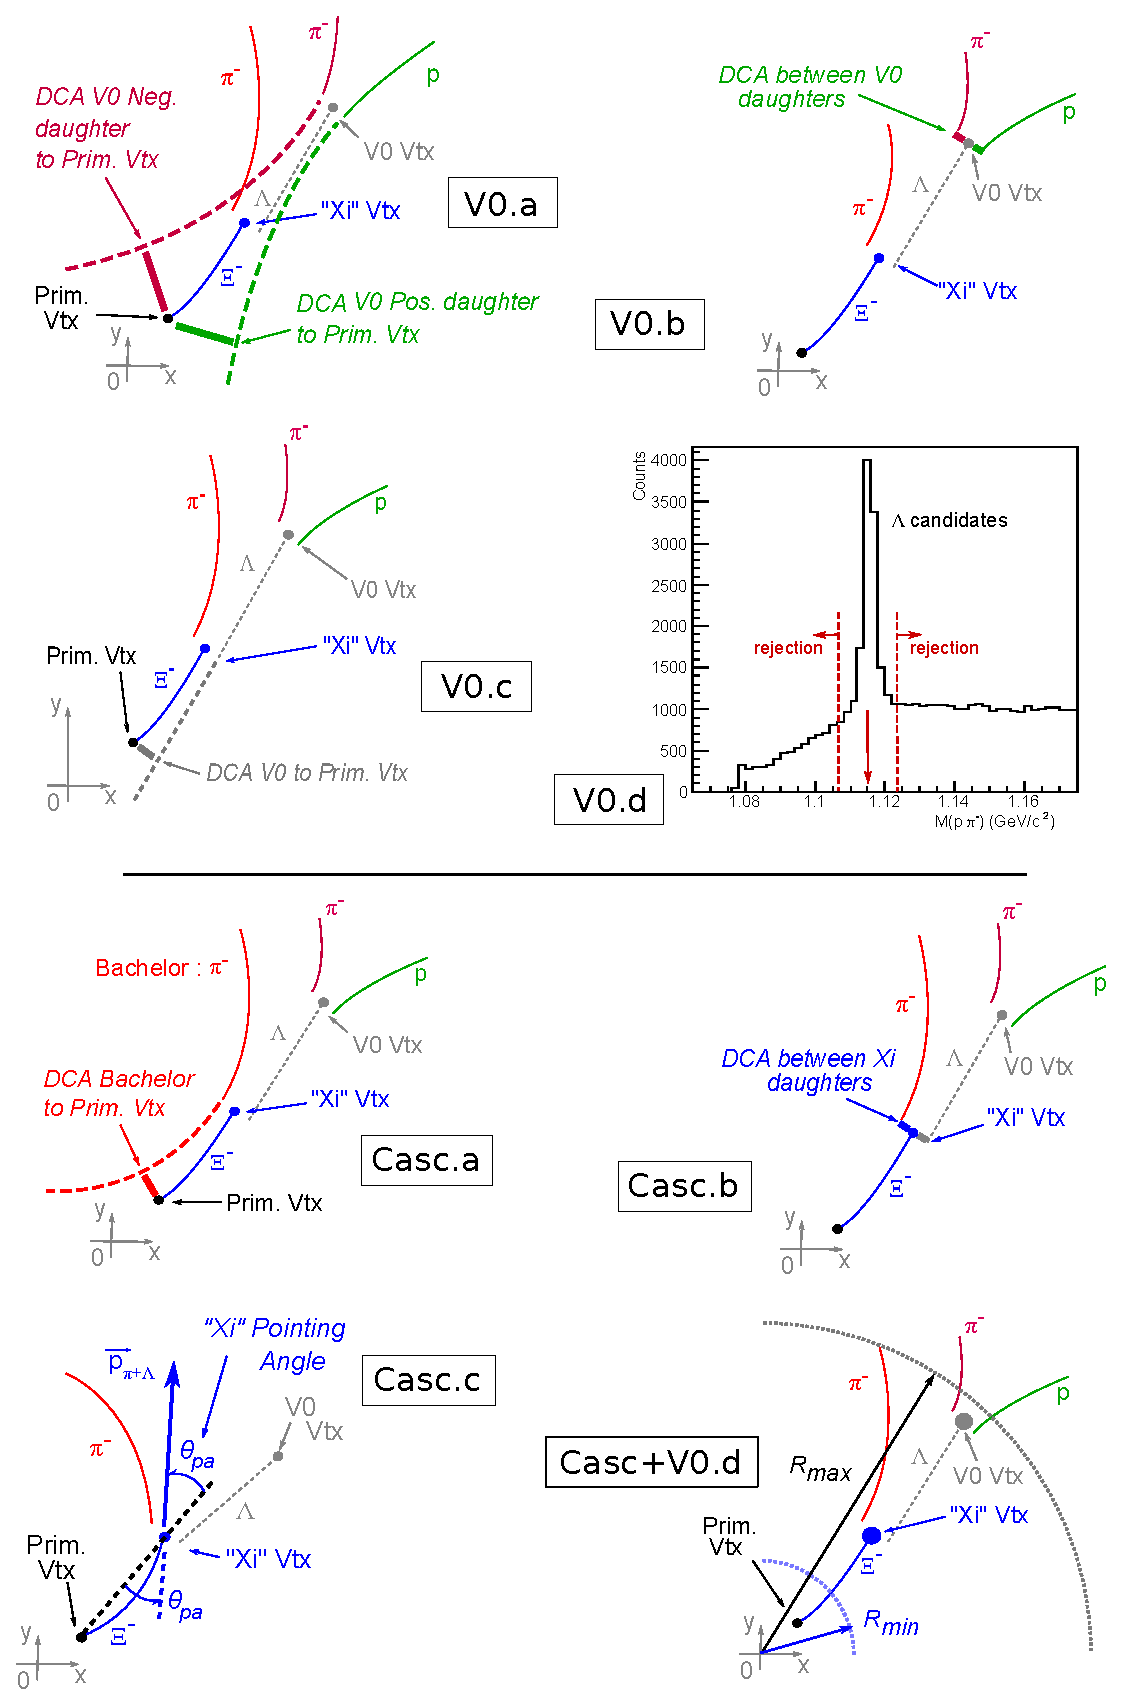
\includegraphics[width=1\textwidth]{Figs/Chapter3/Schema-ExplicationReconstrCascade-en.eps}
	\caption{Schematic representation of the different topological selections applied in order to first reconstruct V0s (top part), and then cascades (bottom part). Figure taken from \cite{maireTopologicalSelectionsV02011}.}
	\label{fig:TopologicalRec}
\end{figure}
}

The two daughter tracks are then propagated from their initial position (the point of closest approach to the primary vertex, \Sec\ref{subsubsec:TrackReco}) to the secondary decay point\footnote{Most importantly, here the propagation is performed without taking the energy losses into account. This point will be addressed in \chap\ref{chap:CPTAnalysis}\label{footnote:EnergyLossV0CascVertexing}}. This allows to calculate all the kinematic quantities of the V0, among which its momentum; the latter being equal to the momentum sum of the positive and negative particles at the secondary vertex, due to momentum conservation.

\subsubsection{The reconstruction of cascade candidates}
\label{subsubsec:CascadeFormation}

From the sample of V0 candidates (\Sec\ref{subsubsec:V0Formation}), only those compatible with a \rmXiPM or \rmOmegaPM decay are considered. In other words, the reconstruction of a cascade candidate must necessarily go through a secondary V0 that corresponds to either a \rmLambda or \rmAlambda.\\

Primary and secondary V0s are separated resorting to the pointing direction in the lab frame, given by the momentum at the decay vertex. This direction coincides with the straight-line trajectory of the candidate\footnote{If the candidate corresponds to an actual \rmLambda or \rmAlambda (electrically neutral), its trajectory, not being curved under the influence of the magnetic field, must necessarily follow a straight line.} and allows to estimate its DCA to the interaction point (\fig\ref{fig:TopologicalRec}, V0.c). The latter being close to zero for primary V0s, a lower cut on this variable enables their rejection to retain only those tagged as secondary. 

The identification of the V0 goes through the calculation of the invariant mass under  the \rmLambda or \rmAlambda hypothesis. This boils down to making an assumption on the mass of each decay daughter. In the case of a \rmLambda, the positive track corresponds to a proton, the negative to a \piMinus (\eq\ref{eq:LambdaInvMass}); conversely, for a \rmAlambda, they are considered as a \piPlus and an anti-proton respectively. If it turns out that the candidate is, in fact, a true \rmLambda or \rmAlambda, the reconstructed mass should lie within a window of typically a few \mmass\footnote{The width of the mass window depends directly on the ALICE performances in terms of transverse \emph{momentum} resolution, which sits around a few \mmom for low- and intermediate-\pT tracks, that is around a 1\%-level resolution. See \fig~\ref{fig:MomResolution} about the track-\pT\ resolution.} (\fig\ref{fig:TopologicalRec}, V0.d), centred around the nominal mass of the \rmLambda,\break $m_{\Lambda} = 1.115683$ \gmass. In most cases, the misidentification of the daughter particles results in a quite different invariant mass. Therefore, only one of the two mass hypothesis passes the cut, making it possible to differentiate between a \rmLambda and a \rmAlambda.

\begin{align}
M_{\rm candidate}^2(\rmLambda) &= ( E_{\rm pos.} + E_{\rm neg.} )^2 - (\vec{p}_{\rm pos.} + \vec{p}_{\rm neg.})^2 \\
&= \Big(\sqrt{ \vec{p}_{\rm pos.}^2 + m_{\rm pos.}^2} + \sqrt{ \vec{p}_{\rm neg.}^2 + m_{\rm neg.}^2}\Big)^2 - ( \vec{p}_{\rm pos.} + \vec{p}_{\rm neg.})^2\\
&= \Big(\sqrt{ \vec{p}_{\rm pos.}^2 + m_{p^{+}}^2}    + \sqrt{ \vec{p}_{\rm neg.}^2 + m_{\pi^{-}}^2}\Big)^2  - ( \vec{p}_{\rm pos.} + \vec{p}_{\rm neg.})^2 \label{eq:LambdaInvMass}
\end{align}

A last step consists in forming a cascade candidate via the association of a candidate \rmLambda (or \rmAlambda) with any track labelled as secondary\footnote{With the exception of the V0 daughters tracks.} (\fig\ref{fig:TopologicalRec}, Casc.a), playing the role of the bachelor particle. The procedure is analogous to what was done to build a V0 candidate: only pairs with a sufficiently small DCA between the reconstructed \rmLambda (or \rmAlambda) and the bachelor are considered (\fig\ref{fig:TopologicalRec}, Casc.b); primary cascades are set apart from secondary ones by introducing the \textit{pointing angle}. The latter corresponds to the angle defined by the direction of propagation (or pointing direction) of the candidate, and the line joining the primary and secondary vertices. This angle should be small for a primary candidate and, even though the magnetic field is bending their trajectory, the change in direction remains moderate. This selection usually goes through the cosine of the pointing angle, that is constrained to be close to unity in order to validate the cascade as primary (\fig\ref{fig:TopologicalRec}, Casc.c).

The V0 candidate is subject to the same cut. Due to its large mass compared to the one of the bachelor, the reconstructed \rmLambda (or \rmAlambda) takes up most of the cascade momentum, and so most of the pointing direction. As a consequence, in order to ensure that the V0 actually originates from a \rmXiPM or \rmOmegaPM decay, the cosine of its pointing angle has to be close to unity.\\

As a final topological selection, the cascade and V0 decay vertices must lie within a certain confidence area, in the transverse plane (\fig\ref{fig:TopologicalRec}, Casc.d). Close to the interaction point, at small radii, the combinatorial background is overwhelming due to the high density of tracks. Conversely, at large distance, the probability of finding a \rmXiPM or \rmOmegaPM becomes extremely low. For comparison, the inner wall of the TPC ($\sim$ 85 \cm) lie at $\sim 18$ $\cTau_{\Xi}$ and $\sim 35$ $\cTau_{\Omega}$. At such distance, the \rmXiPM and \rmOmegaPM survival probabilities are about 2\% and 0.001\%\footnote{Considering a high-momentum cascade of 5 \gmom.} respectively. Therefore, the decay vertices of both cascade and V0 must be located beyond a radius deemed critical; those decaying too far away with respect to their lifetime are rejected\footnote{Note that one consists in a selection on the \emph{radial} position of the decay vertices, the other, in a cut on their \emph{3D} location.}.

\subsubsection{Invariant mass of the cascade candidates}
\label{subsubsec:InvariantMassSelection}

At this stage, the topological reconstruction is over; each triplet of tracks forms a cascade candidate, that can correspond to a \rmXiPM, a \rmOmegaPM or some residual background. The distinction is made based on the invariant mass of each candidate (\eq\ref{eq:CascInvMass}).


\begin{align}
M_{\rm candidate}^2( \textrm{casc.}) &= ( E_{\rm V0} + E_{\rm bach.} )^2 - ( \vec{p}_{\rm V0} + \vec{p}_{\rm bach.})^2 \\
&= \Big(\sqrt{ \vec{p}_{\rm V0}^2 + m_{\rmLambda}^2} + \sqrt{ \vec{p}_{\rm bach.}^2 + m_{\rm bach.}^2}\Big)^2 - ( \vec{p}_{\rm V0} + \vec{p}_{\rm bach.})^2 \label{eq:CascInvMass}
\end{align}

\begin{align}
M_{\rm candidate}^2( \rmXiPM ) &= \Big(\sqrt{ \vec{p}_{\rm V0}^2 + m_{\rmLambdaPM}^2} + \sqrt{ \vec{p}_{\rm bach.}^2 + m_{\pi^{\pm}}^2}\Big)^2 - ( \vec{p}_{\rm V0} + \vec{p}_{\rm bach.})^2 \label{eq:XiInvMass} \\
M_{\rm candidate}^2( \rmOmegaPM ) &= \Big(\sqrt{ \vec{p}_{\rm V0}^2 + m_{\rmLambdaPM}^2} + \sqrt{ \vec{p}_{\rm bach.}^2 + m_{\rm K^{\pm}}^2}\Big)^2 - ( \vec{p}_{\rm V0} + \vec{p}_{\rm bach.})^2
\label{eq:OmegaInvMass}
\end{align}

For each association of three particles (\ie one cascade candidate), two invariant masses are calculated: one under the hypothesis of a \rmXiPM candidate (\eq\ref{eq:XiInvMass}), the other for a \rmOmegaPM candidate (\eq\ref{eq:OmegaInvMass}). Note that, contrarily to the \rmLambda and \rmAlambda cases, the numeric value of the invariant mass is the same for the \say{particle} (\rmXiM, \rmOmegaM) and the \say{anti-particle} calculations (\rmAxiP, \rmAomegaP). The mass roles do not swap among the two decay daughters, V0 and bachelor; only the sign of the bachelor's electric charge allows to distinguish between particle and anti-particle. In addition, the masses of the daughter particles involved in \eq\ref{eq:XiInvMass} and \ref{eq:OmegaInvMass} correspond, in fact, to the nominal values from the PDG \cite{particledatagroupReviewParticlePhysics2022}; most importantly, that means that the reconstructed mass of the V0 is not being used here, \ie the PDG mass \mPDG[\rmLambda] is used instead. As long as the latter has been identified as a \rmLambdaPM (\ie its mass fits into a certain tolerance window, \Sec\ref{subsubsec:CascadeFormation}), this choice has the advantage of limiting the deterioration on the cascade invariant mass resolution. \\

Although the invariant mass allows to distinguish a \rmXiPM from a \rmOmegaPM, there exists a region where this is not possible anymore. \Fig\ref{fig:MassXiVsOmega} shows the invariant mass distribution of cascade candidates assuming a \rmOmegaM as a function of the same candidate under the hypothesis of a \rmXiM. There are two discernible and perpendicular mass bands, each one corresponding to true population of one of two considered species. At their intersection, the two species become indistinguishables -- they compete, in some sense -- which results in an increased background in this region: a candidate identified as \rmXiM may, in fact, reveal to be a \rmOmegaM, and vice-versa.

This additional background affects each kind of cascade in different proportions, though. Since the population of true \rmXiM is much larger than the one of \rmOmegaM\footnote{That is because the \rmXi are typically ten times more produced than the \rmOmega~\cite{alicecollaborationProductionLightflavorHadrons2021}.}, the latter constitutes a marginal source of background with respect to the \rmXiM. Conversely, the true \rmXiM -- particularly in the low mass region -- represent a considerable source of background for the \rmOmegaM. As a consequence, in the context of the reconstruction of \rmOmegaPM baryons, any candidates also identified as a \rmXiPM\ --- that is, with an invariant mass under the assumption of a \rmXiPM within a window of few \mmass around \mPDG[\rmXi]\ --- are rejected.

\begin{figure}[!t]
	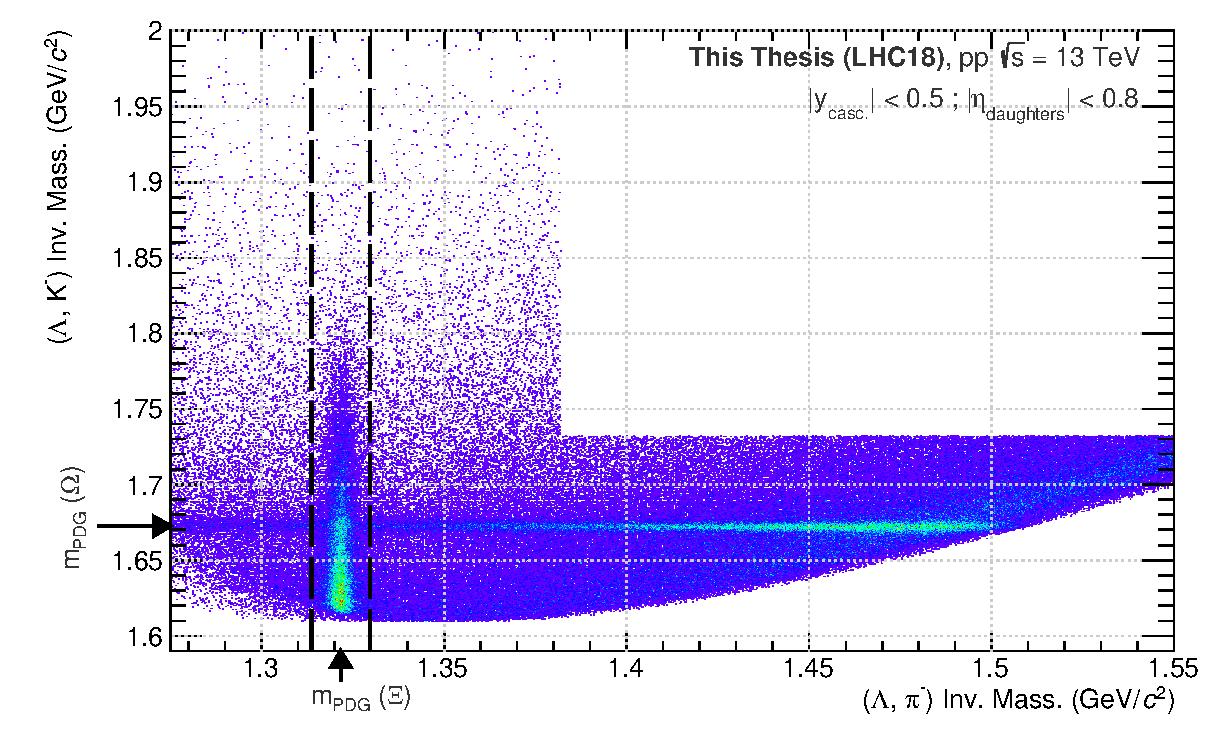
\includegraphics[width=0.9\textwidth]{Figs/Chapter4/MassXiVsOmegaMinus.eps}
	\caption{Invariant mass distribution under the \rmOmegaM and \rmXiM mass hypotheses, each cascade candidate can be seen under one hypothesis or the other (\eq\ref{eq:XiInvMass} and \ref{eq:OmegaInvMass}). The dashed lines show the mass rejection $\mPDG[\rmXi] \pm 0.008~\gmass$, applied in the reconstruction of a \rmOmegaPM candidate.}
	\label{fig:MassXiVsOmega}
\end{figure}



\subsection{The context of hyperon reconstruction in ALICE}
\label{subsec:HyperonAndALICE}

In view of their characteristics, the reconstruction of multi-strange baryons requires excellent detection capabilities. In that regard, few experiments can compete with the performances of the ALICE detector at mid-rapidity.

As already outlined in \Sec\ref{subsec:ALICEDetector}, the high granularity of its inner tracker allows to reconstruct the primary vertex, as well as the secondary vertices from V0 and cascade decays, with a precision better than 100 \mum\footnote{Not to mention the resolution on the DCA of the daughter tracks to the primary vertex of about 30 \mum \cite{alicecollaborationPerformanceALICEExperiment2014}.}. Thanks to its large lever arm and almost continuous sampling of the particle trajectory, the TPC 
provides an excellent momentum measurement with a resolution of 0.7\%\footnote{This obviously depends on the track momentum; here this is for \pT = 1 \gmom.} \cite{alicecollaborationALICEPhysicsPerformance2006}, as well as a robust particle identification. Hence, the TPC ensures an efficient reconstruction and identification of the hyperon's decay daughters, and thus of the hyperon itself. Coupled with its extremely low material budget (13\% \Xzero\ up to the upper wall of TPC) and moderate magnetic field of 0.5 T, the strange hadron reconstruction can be performed over a wide momentum range and particularly, at low \pT, where the most important part of the production is.

Furthermore, the experiment benefits from the high-energy collisions delivered by the LHC. At such energies, matter and anti-matter are produced in almost equal proportions, offering the opportunity to study simultaneously hyperons and anti-hyperons. For all these reasons, ALICE stands as a perfectly suited experiment to analyse multi-strange baryons. \\

It should be emphasized that the cascade reconstruction varies with the track density, that goes from a few charged particles in pp collisions up to 2000 in the most central Pb-Pb collisions at \sqrtSnn = 5.02 \tev \cite{alicecollaborationCentralityDependenceChargedParticle2016}. In heavy-ion collisions, the enormous amount of tracks means a larger background, but also a larger number of contributor for the primary vertex determination and hence a better resolution on its position. This is in contrast with the pp environment, where the events are less dense but the quality of the primary vertex reconstruction is poorer. Therefore, the topological selections shall be adapted for each environment, as these differences may lead to various biases on the DCA to the primary vertex, pointing angles, etc.

Also, a compromise has to be made between purity and reconstruction efficiency. In both cases, the key point revolves around the treatement of the background, which depends on the physics analysis. For example, if the background -- or more precisely, its shape -- is known in advance, the latter becomes tolerable as it can be subtracted later; thus, one may favour a high efficiency (\ie relatively loose selections). In the reverse situation  where the background is unknown, it seems preferable to apply tighter cuts in order to keep a signal with a low level of contamination, thus ensuring a high signal purity.

 % V0 and cascade reconstruction
%//------ Section 03 -------------------------------------------------------------------------------------------------
\chapter{Mass measurements of multi-strange baryons in pp collisions at \sqrtS = 13 TeV}
\label{chap:CPTAnalysis}
%//-----------------------------------------------------------------------//

The first analysis conducted in this thesis aims at measuring the masses and mass differences between particle and anti-particle of multi-strange baryons. The focus is on \rmXiM, \rmAxiP, \rmOmegaM and \rmAomegaP. This chapter provides a description of the different elements needed to achieve this goal. 

\section{Introduction}

%Symmetries certainly stand as one of the most fruitful concepts in Physics. They are of two kinds: continuous --- such as the global translations in both space and time, or the Lorentz transformations --- and discrete --- for example, the space- (P) and time- (T) inversions, the charge conjugation (C), and their combined transformation given by CPT. In particular, the Lorentz and CPT symmetries are connected by the so-called CPT theorem which states that any local Lorentz-invariant quantum field theory must also (under some extra requirements) be CPT invariant \cite{cptstatus}. Consequently, the CPT violation implies the breaking of the Lorentz symmetry, and vice versa\footnote{In fact, there is another option; to allow for CPT to be violated, either the Lorentz symmetry must be broken -- as in the string theory \cite{string} or the Standard-Model Extension \cite{sme} -- or some of the other extra assumptions of the CPT theorem must be dropped, namely the energy positivity, local interactions, finite spin, etc \cite{cptimplieslorentz}\cite{cptsymmetryantitsviolation}. } \cite{sozzi}. Another implication involves the relation between the properties of matter and antimatter: due to the charge conjugation linking particles to antiparticles, the CPT symmetry imposes that they share the same invariant mass, energy spectra, lifetime, coupling constants, etc \cite{cptsymmetryantitsviolation}. Most of the experimental checks of CPT invariance stem from these physical consequences.

As discussed in \Sec\ref{subsec:Theory}, the Standard Model is built upon a set of symmetries, each being either discrete -- such as the combination of the charge conjugation (C), parity (P) and time reversal (T), known as the CPT transformation -- or continuous -- for example, the Lorentz transformations that includes rotations and boosts. In particular, the Lorentz and CPT symmetries are connected by the so-called CPT theorem which establishes that any unitary, local Lorentz-invariant quantum field theory must be CPT invariant \cite{kosteleckyStatusCPT1998}. Consequently, the CPT violation implies the breaking of the Lorentz symmetry, and vice versa\footnote{In fact, another option exists; to allow for the CPT violation, either the Lorentz symmetry must be broken -- as in the case of string theory \cite{kosteleckySpontaneousBreakingLorentz1989} or the Standard-Model Extension \cite{colladayLorentzviolatingExtensionStandard1998} -- or some of the other additionnal assumptions of the CPT theorem must be dropped, namely the energy positivity \cite{abersDiseasesInfiniteComponentField1967}, local interactions \cite{carruthersIsospinSymmetryTCP1968}, finite spin \cite{oksakInvalidityTCPtheoremInfinitecomponent1968}, etc \cite{greenbergCPTViolationImplies2002}\cite{lehnertCPTSymmetryIts2016}. } \cite{sozziTestsDiscreteSymmetries2019}. Another implication involves the relation between the properties of matter and antimatter: due to the charge conjugation linking particles to antiparticles, the CPT symmetry imposes that they share the same invariant mass, energy spectra, lifetime, coupling constants, etc \cite{cptsymmetryantitsviolation}. Most of the experimental checks of CPT invariance stem from this last point, which imposes several constraints on the anti-particle properties. \\

The Particle Data Group (PDG) \cite{particledatagroupReviewParticlePhysics2022} compiles a large variety of CPT tests from many experiments and with different degrees of precision; so far, no CPT violation has been observed. The most stringent test involves the \rmKzero-\rmAKzero mixing process, which depends on the mass and lifetime differences of these two states. In this way, assuming no other source of CPT violation in the decay of neutral kaons, these two quantities have been bounded \cite{particledatagroupReviewParticlePhysics2022}\cite{angelopoulosK0K0Mass1999} to 

\begin{equation}
2 \frac{\mid m_{\rmKzero} - m_{\rmAKzero} \mid}{m_{\rmKzero} + m_{\rmAKzero}} < 6 \times 10^{-19} \quad , \quad 2 \frac{\mid \Gamma_{\rmKzero} - \Gamma_{\rmAKzero} \mid}{\Gamma_{\rmKzero} + \Gamma_{\rmAKzero}} = (8 \pm 8) \times 10^{-18}.
\end{equation}

These indirect limits are much stronger than the ones extracted from direct tests. For example, in the hyperon sector, the precision on relative mass difference is typically of a few $10^{-5}$. In the latter case, it should be mentioned that there is still some room for improvements, and most particularly concerning the mass difference measurements between particle and anti-particle in the multi-strange baryon sector. The only test of this nature dates back to 2006 \cite{abdallahMassesLifetimesProduction2006} for the \rmXiM and \rmAxiP, and from 1998 \cite{chanMeasurementPropertiesOverline1998} for the \rmOmegaM and \rmAomegaP. The former was achieved by exploiting 3.25 million hadronic decays of the \rmZzero recorded by the DELPHI detector at LEP-1; the latter was obtained on the E756 spectrometer at Fermilab, using an 800-\gmom proton beam on a beryllium target. However, both studies suffer from low statistics: approximately 2500(2300) reconstructed \rmXiM (\rmAxiP) and about 6323(2607) reconstructed \rmOmegaM (\rmAomegaP) were used.\\

\begin{table}[t]
    \centering
    \begin{tabular}{>{\centering\arraybackslash}b{1.5cm}@{\hspace{0.3cm}} >{\centering\arraybackslash}b{1.75cm}@{\hspace{0.3cm}} >{\centering\arraybackslash}b{2.85cm}@{\hspace{0.3cm}} >{\centering\arraybackslash}b{3.6cm}@{\hspace{0.3cm}} >{\centering\arraybackslash}b{2.5cm}@{\hspace{0.3cm}} >{\centering\arraybackslash}b{1cm}@{\hspace{0.3cm}}}
    \noalign{\smallskip}\hline\noalign{\smallskip}
	Particle & Quark content & Mass (\mmass) & Relative mass difference & Dominant decay channel & B.R.\\	
    \noalign{\smallskip}\hline \noalign{\smallskip}
    	
	\rmKzeroS (\rmAKzeroS) & $d \bar{s}$ ($\bar{d} s$)& $497.611 \pm 0.013$ & $< 6 \times 10^{-19}$ & \piPlus \piMinus & 69.20\%\\
	
    \noalign{\smallskip}\hline \noalign{\smallskip}
    
    \rmLambda (\rmAlambda) & $u d s$ ($\bar{u}\bar{d}\bar{s}$) & $1115.683 \pm 0.006$ & $\left(-0.1 \pm 1.1\right) \times 10^{-5}$ & \proton \piMinus (\pbar \piPlus) & 63.9\% \\
    
    \noalign{\smallskip}\hline \noalign{\smallskip}    
    
    \rmXiM (\rmAxiP) & $dss$ ($\bar{d}\bar{s}\bar{s}$) & $1321.71 \pm 0.07$ & $\left(-2.5 \pm 8.7\right) \times 10^{-5}$ & \rmLambda \piMinus (\rmAlambda \piPlus) & 99.9\% \\	
    \noalign{\smallskip}\hline \noalign{\smallskip}
    
	\rmOmegaM (\rmAomegaP) & $sss$ ($\bar{s}\bar{s}\bar{s}$) & $1672.45 \pm 0.23$ & $\left(-1.44 \pm 7.98\right) \times 10^{-5}$ & \rmLambda \rmKminus (\rmAlambda \rmKplus) & 67.8\%\\    
    \noalign{\smallskip}\hline\noalign{\smallskip}
    \end{tabular}
    \caption{A few characteristics, as of 2023, of the \rmLambda, \rmXi, \rmOmega hyperons and the \rmKzeroS meson: quark content, mass, relative mass difference values with their associated uncertainties and their dominant decay channel as well as the corresponding branching ratio \cite{particledatagroupReviewParticlePhysics2022}.}\label{tab:V0CascPDGMass}
\end{table}

In comparison, all the pp collisions at a centre-of-mass energy of 13 \tev collected by ALICE throughout the LHC Run-2 contains about 2 500 000 \rmXi and 133 000 \rmOmega, with little background. Therefore, in this thesis, the measurement of the mass difference of \rmXiM and \rmAxiP, and \rmOmegaM and \rmAomegaP hyperons is performed. It relies on data samples much larger than those exploited previously. These direct measurements of the mass difference should offer a test of the CPT invariance to an unprecedented level of precision in the multi-strange baryon sector. The absolute masses are updated as well, with a precision substantially better than the past measurement, currently listed in the PDG and presented in the \tab\ref{tab:V0CascPDGMass}.

Furthermore, concerning the \rmLambda hyperon and \rmKzeroS meson, the PDG quotes a precision of a few \kmass on the mass value, and about $1 \times 10^{-5}$ on the relative mass difference value\footnote{This only concerns the relative mass difference between \rmLambda and \rmAlambda. As mentioned above, such quantity is much smaller by fourteen orders of magnitude in the case of \rmKzero.}. Abundantly produced, these two hadrons also exhibit an irresistible feature in the context of this thesis: both decay into a V0 in their dominant decay channel, and so can be identified in a similar manner as cascades using topological reconstruction. For those two reasons -- high precision on the PDG mass values, and similar decay topology as cascade --, the analysis is reproduced on \rmLambda and \rmKzeroS, both being used as a benchmark for the measurement.\\

In the following, the term \textit{mass difference} always refers to the \emph{relative} one  -- unless indicated otherwise --, namely the mass \emph{difference} over the mass \emph{average}, $2 \left(\mMassPart{part.} - \mMassApart{part.} \right)/\left(\mMassPart{part.} + \mMassApart{part.}\right)$.

\section{Data samples and event selection}

\subsection{The data samples}
\label{subsec:DataSamples}

All the data samples employed for this measurement originates from the second campaign of data taking, the LHC Run-2. These samples comprise different collision systems at various energies, mainly pp collisions at \sqrtS = 13 \tev and Pb-Pb collisions at \sqrtSnn = 5.02 \tev. Based on the elements in \Sec\ref{subsec:HyperonAndALICE}, the analysis exploits the pp collisions as they provide a less dense collision environment, expectedly easier to reconstruct and thus more controllable. All these pp events have been collected during three data taking periods: between April and October 2016, May and November 2017, April and October 2018 (\Sec\ref{subsec:acceleratorprogramme}, \tab\ref{tab:LHCRunProgramm}).

Considering the target precision on the mass and mass difference values, it is crucial to have a fine comprehension of the data reconstruction to keep it well under control. For that reason, the analysis uses data in ESD format as they contain all the informations related to event building, thus offering the possibility to replay \textit{offline} the V0 and cascade vertexings/formations. As mentioned in \Sec\ref{subsubsec:DataFormats}, the first full reconstruction cycle (\Sec\ref{subsubsec:computingmodel}), performed right after their recording of the data, produces ESD files labelled as \textit{pass-1}. Since then, other reconstruction cycles have been carried out, each iteration bringing its share of improvements or fixes. The events analysed for this measurement originates from the second reconstruction cycle, the \emph{pass-2}, which offers better tracking performances: same and consistent version of analysis software over all the data taking periods leading to more uniform performances, better SPD and TPC alignments, improved TPC reconstruction and finer description of the distortions within the TPC gas.

Each period consists in fact of dozens or hundreds of \textit{runs}, corresponding to sequences of events recorded in an uninterrupted manner\footnote{Throughout the data taking, it is more or less frequent to interrupt the data collection, \ie stop the run. This usually occurs when a detector encounters an error, unfixable while collecting data. Broadly speaking, a period regroups a set of runs that have been recorded within the same data taking conditions.}. The lists of appropriated runs for physics analysis are defined by the ALICE Data Preparation Group (DPG). As its name suggests, the latter oversees the preparation, reconstruction, quality assurance of both collected and simulated data, as well as the upkeep of the analysis tools including the event and track selections \cite{alicecollaborationALICEDataPreparation2023}. The list of runs employed in this study follows the DPG's recommendations for an analysis using central barrel detectors and requiring hadron PID. For a run to be in that list, all the detectors related to the tracking and PID must be operational -- \ie SPD, SDD, SSD (ITS), TPC, TOF --, as well as those in charge of triggering, that are the V0 and T0. Note that it does not mean that the PID performances are optimal, nor that the full acceptance of each detector is covered.\\

Besides the real data sample, the measurement also relies on simulated data in order to estimate and optimize the performances of the analysis. To each run corresponds its simulated counterpart, anchored on pass-2 data, as described in \Sec\ref{subsubsec:MCData}. All the exploited MC productions employ \Pythiaeight (version 8.2, tune: Monash 2013) as event generator. For the transport and interaction with the material of the ALICE detector, most of them use \GeantThree; although \GeantFour describes more accurately hadronic interactions at very low momentum and is better maintained, only a few of simulations rely on it, because of its higher consumption of computing resources \cite{barendsGeant4ValidationStudy2017}. 

Since both abundant (\rmKzeroS, \rmLambda and to a certain extent, \rmXi) and rare species (\rmXi and \rmOmega) are being studied, one may resort to two kinds of simulations: general-purpose MC productions for the first ones, and enriched MC productions for the others. Here, the enriched simulations have been obtained by selecting the events that include, at least, a \rmKzeroS, \rmLambdaPM, \rmXiPM or \rmOmegaPM in $\abspseudorap < 1.2$. It turns out that most of the studies carried out in the present analysis use on the latter simulations because of i) the enrichment in strangeness, ii) they cover all the periods of the considered LHC Run-2 data, and iii) they use \GeantFour.

Furthermore, this analysis also makes use of the track references in the simulation. As mentioned in \Sec\ref{subsubsec:MCData}, these correspond to the MC informations of the considered track at the location where it crosses a given detection plane. Thereby, they allow for comparing the reconstructed track properties with the actual/generated ones at any point along the particle trajectory\footnote{Strictly speaking, this comparison cannot be done at any point since the track reference is only available where the particle traverses a sensitive volume.}. Although the track references are effectively stored for only 10\% of the production\footnote{This is done in order to spare some disk space.}, this comparison is proving invaluable to control the tracking in ALICE.\\


In total, the exploited data sample counts about 2.6 billions minimum bias events at \sqrtS = 13 \tev, and approximately 600 millions events in the associated MC productions.

\subsection{The event selection}
\label{subsec:EventSelection}

As mentioned in \Sec\ref{subsec:TriggerSystem}, the analysis focuses on minimum-bias and/or high-multiplicity events. More precisely, the respective trigger configurations correspond to the MB$_{\rm AND}$ and/or HM$_{\rm VZERO}$. Not all the events passing these trigger selections are considered; additional cuts are applied in order to filter out only those of \say{good} quality suitable for a physics analysis. \\

During the data acquisition (DAQ), the event-builder proceeds to the event reconstruction based on the sub-events from all contributing detectors. It may happen, however, that a detector's output cannot be transmitted due to the associated data channel being closed\footnote{There are different reasons for the data channel to be closed. At the beginning or the end of each run, a specific procedure is performed on all detectors in order to effectively initiate the start or stop of the run. In particular, the \say{End Of Run} procedure has to close all the data channel connecting the event-builder and the sub-detectors -- \ie the GDCs and LDCs respectively (\Sec\ref{subsec:TriggerSystem}) --, but this termination can occur sooner in the case of a connection time-out for example.} \cite{alicecollaborationTriggerDataAcquisition}. The event-builder still reconstructs the event, although it is tagged as \say{incomplete DAQ} due to the missing informations. Such events are rejected in the present work.\\

There exists three types of reconstructed primary vertex in ALICE, from the highest to the poorest quality: one estimated using the global ITS-TPC tracks (\Sec\ref{subsubsec:FinalVertexDet}), another based on the SPD tracklets (\Sec\ref{subsubsec:PreliminaryVertex}), and the last optional one built from the TPC standalone tracks in a similar way as the former. By default, only the \say{best} available reconstructed primary vertex is considered. 

Nevertheless, to ensure that the event has a vertex of a sufficiently good quality, the analysis relies exclusively on the first two aforementioned primary vertices. This boils down to requiring the presence of, at least, the one reconstructed using tracklets\footnote{As mentioned in \Sec\ref{subsubsec:PreliminaryVertex}, the event cannot be built without the primary vertex based on SPD tracklets. Hence, by construction, the presence of such vertex is guaranteed in the event.}. Moreover, the resolution of the latter in the longitudinal direction should not exceed 0.25 \cm. In cases when both SPD tracklets and global ITS-TPC track vertices are available, their positions along the beam axis must coincide within a 0.5-\cm window.

As a prerequisite for guaranteeing a uniform reconstruction efficiency, particles must remain within the acceptance of all the central detectors involved in their reconstruction, that is $\abspseudorap < 0.9$. For particles originating from the interaction point, this condition implies a constraint on the longitudinal position of the primary vertex: the absolute distance between the interaction point and the centre of ALICE should be below 10 \cm along the beam axis\footnote{Note that there is no selection of such nature concerning the \emph{transverse} position of the primary vertex, except that it must be located below the beam pipe.}. \\

A key element of the event quality concerns the pile-up level. The latter occurs when there are two or more collisions coming from the same bunch crossing -- this is the \textit{in-bunch} pile-up -- and/or from different bunch crossings occuring within the readout time of the detectors -- also called \textit{out-of-bunch} pile-up. One approach to remove both types of pile-up consists in rejecting events with multiple reconstructed primary vertices. This selection depends on the nature of the best primary vertex available.
\begin{itemize}
\item[$\bullet$] If it is the one reconstructed using ITS-TPC tracks, the event selection algorithm checks the presence of another primary-like vertex of reasonably good quality ($\rmChiSquareNDF < 5$, with $NDF$ the number of degrees of freedom), formed out of at least five tracks, and separated from the first one by more than $15 \sigma$\footnote{Here, $\sigma$ denotes the uncertainty on the distance between the two vertices.}. If such vertex exists, the event is discarded. 
\item[$\bullet$] Otherwise, it corresponds to the one built from SPD tracklets. To maximise the selection efficiency, the cuts adapt to the tracklet multiplicity. Hence, if a second vertex is found to be away from the first one by more than 0.8 \cm along the beam axis, with at least three, four or five associated tracklets for a total number of reconstructed tracklets (\rmNTracklet) inferior to 20, $20 < \rmNTracklet \leq 50 $ and \rmNTracklet > 50 respectively, then the event is rejected.
\end{itemize}


Along the same line, the two innermost layers of the ITS can help to identify the remaining beam-induced background -- that have not been removed by the MB$_{\rm AND}$ trigger selection -- and pile-up events. As mentioned in \ref{subsubsec:PreliminaryVertex}, a tracklet is formed out of pair of clusters found in the two SPD layers, separated by an angle of 0.01 rad at most. Therefore, if the number of clusters increases, so does the amount of reconstructed tracklets. However, in the case of beam-gas event, there should be many clusters but only a small number of tracklets could be formed using the previous definition. In pile-up events, only the tracklets associated with the primary vertex are considered; for that reason, the number of clusters should be relatively larger than expected at such tracklet multiplicity \cite{alicecollaborationALICEPhysicsForum2016}. In this way, based on this correlation between the number of SPD clusters and tracklets, the remaining events flagged as background or pile-up are rejected. \\

\begin{figure}[t]
	\centering
	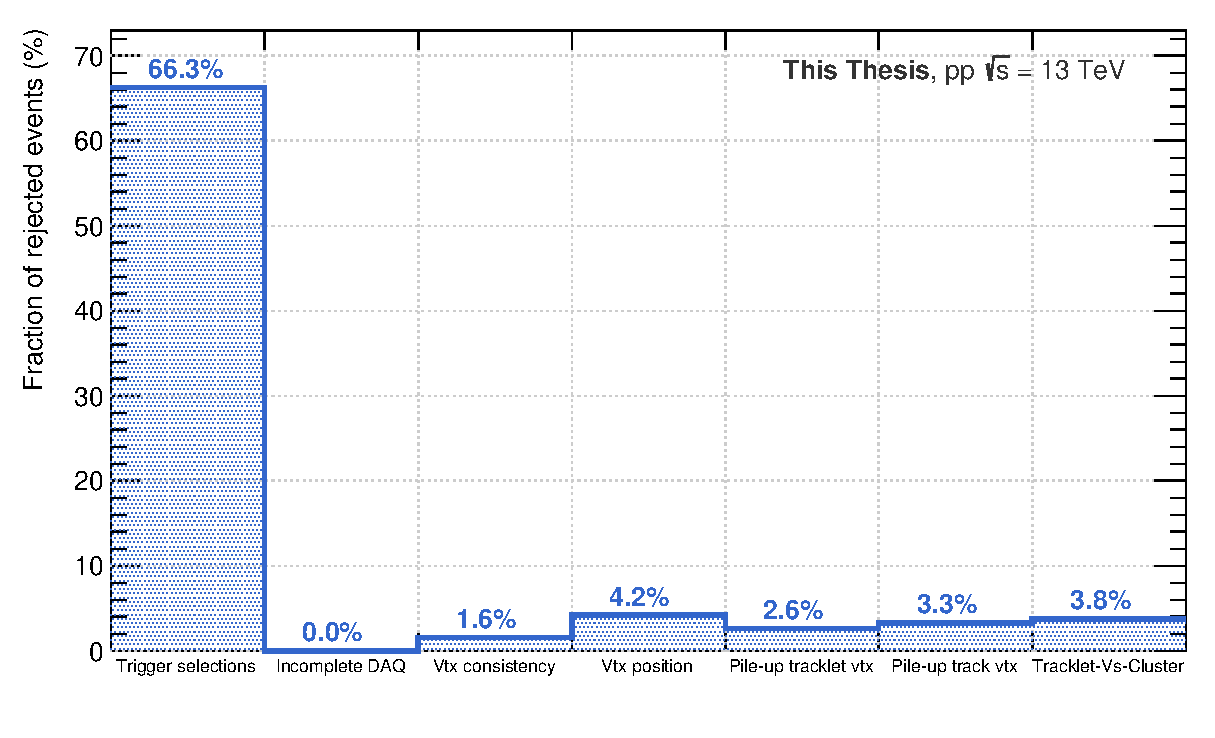
\includegraphics[width=1\textwidth]{Figs/Chapter5/EventSelection.eps}
	\caption{Fraction of rejected events in the present data sample for each event selection independently of the others: trigger selections (MB$_{\rm AND}$ and/or HM$_{\rm VZERO}$), incomplete DAQ, consistency between the global track and SPD tracklet vertices, longitudinal position of the primary vertex ($\mid \Delta z \mid < 10 $ \cm), pile-up removal for SPD tracklet and ITS-TPC track vertices, correlation between SPD tracklets and clusters.}
	\label{fig:EvtSelection}
\end{figure}


The \fig\ref{fig:EvtSelection} provides the fraction of rejected events as a function of the above selections in pp collisions at \sqrtS = 13 \tev.

\section{Analysis of the hyperon masses}

\subsection{Track selections}
\label{subsec:TrackSelections}

The identification of V0s and cascades strongly depends on the reconstruction quality of the daughter tracks, and more precisely on their momentum resolution and trajectory. For that reason, the strange particle reconstruction relies exclusively on ITS-TPC combined tracks, since they offer the best momentum resolution as discussed in \Sec\ref{subsubsec:TrackReco} and shown in \fig\ref{fig:MomResolution}. In order to ensure an excellent momentum resolution as well as a fine estimation of the particle trajectory, various selection criteria are applied on the daughter tracks.\\

The analysis concentrates exclusively on tracks comprised within the pseudo-rapidity region $\abspseudorap < 0.8$. The latter corresponds to the acceptance volume of all the central detectors, which provides a constant reconstruction efficiency. Moreover, any track containing ITS and/or TPC shared clusters is rejected, as they potentially correspond to wrongly assigned clusters that could bias the tracking quality. 

Tracks belonging to a \textit{kink} vertex are discarded from the analysis, as they most certainly do not originate from a cascade decay and thus represent an additional source of combinatorial background. A kink usually happens when a charged particle decays into a neutral and a charged particle, such as $\Kplusmin \rightarrow \rmNeutrinoMu \muPlusMinus$. The former being undetected, they are identified by forming pairs of tracks, that intersect in space with a large angle and share the same electric charge.

Each track should have passed the final refit in the TPC. This means that its parameters have been estimated successfully in the TPC during the third stage of the tracking, when the track is re-propagated inwards to their distance of closest approach to the primary vertex (\Sec\ref{subsubsec:TrackReco}). To guarantee a good momentum resolution and a stable particle identification (PID) based on the energy deposit (\dEdx) in the TPC, the tracks need to be associated to at least 70 readout pad rows in the TPC out of 159 possible in total. These selections eliminate the contribution of short tracks and, incidentally, pairs of tracks formed out of the clusters from a single actual particle.\\

The reconstruction of V0s and cascades presented in \chap\ref{chap:V0CascReconstruction} does not resort to any kind of selections on the nature of the daughter particles, apart from their electric charge. This yields \textit{de facto} to an outstanding amount of background candidates. One way of suppressing the latter with a minimal cost in terms of signal candidates consists in using the PID informations provided by the TPC. In practice, the idea is to reject every association that involves tracks inconsistent with the expected identities for either a \rmKzeroS, \rmLambdaPM, \rmXiPM or \rmOmegaPM decay.

As explained in \Sec\ref{subsubsec:TPC}, a track can be labeled as a pion, proton or kaon by making use of the PID estimator in \eq\ref{eq:PIDEstimator}, \Nsigma, which evaluates the difference between the measured \dEdx and the expected one under a given particle mass hypothesis in units of relative resolution. The separation power of such estimator evolves with the particle momentum which, in turn, influences the selection threshold and has some implications in terms of purity and efficiency: the tighter the selection on \Nsigma, the higher the purity but at the price of a smaller efficiency; conversely, a looser cut on \Nsigma deteriorates the purity in favour of a higher efficiency.

The identification strategy adopted here consists in selecting only the tracks compatible with their expected mass hypothesis within \Nsigma = $\pm 3$ at most. This selection is applied on \emph{each} decay daughters, irrespective of their momentum or the one of the mother particle. Considering the \rmXiM or \rmOmegaM case, this imposes that:
\begin{itemize}
\item[$\bullet$] the bachelor track must be consistent with the \rmPiMinus or \rmKMinus mass hypothesis, in the case of \rmXiM or \rmOmegaM respectively,
\item[$\bullet$] the positive track needs to be compatible with a proton hypothesis,
\item[$\bullet$] and the negative track has to agree with energy loss band of the pion.
\end{itemize}
In the case of \rmAxiP or \rmAomegaP, one needs to swap the electric charge of the  decay daughters, namely the positive track needs to be compatible with a pion hypothesis and the negative track, an anti-proton. For the \rmKzeroS, both positive and negative tracks should be compatible with the pion hypthesis.


\subsection{V0s and cascades selections}
\label{subsec:V0CascSelections}

\subsubsection{Topological and kinematic selections}

Once the events and tracks have been selected, the topological reconstruction of V0s and cascades comes into play, as explained in \chap\ref{chap:V0CascReconstruction}. However, not all the candidates are considered in the analysis. As suggested in \Sec\ref{subsec:HyperonAndALICE}, ALICE is well suited for studying hyperons but only at mid-rapidity. This means that the V0s and cascades are reconstructed in the rapidity window $\absrap < 0.5$.

\begin{table}[t]
    \centering
    \begin{tabular}{c|c|c}
    \noalign{\smallskip}\hline \noalign{\smallskip}
    \bf Candidate variable & Selections \rmLambdaPM & Selections \rmKzeroS \\
    \noalign{\smallskip}\hline \noalign{\smallskip}    
    V0 \pT interval (\gmom) & \multicolumn{2}{c}{1 < \pT < 5} \\
    V0 rapidity interval & \multicolumn{2}{c}{\absrap < 0.5} \\
    Competing mass rejection (\gmass) & > 0.010 & > 0.005 \\
    MC association (MC only) & \multicolumn{2}{c}{Correct identity assumption} \\ 

    \noalign{\smallskip} \hline \noalign{\smallskip}
    \bf Track variable & Selections \rmLambdaPM & Selections \rmKzeroS \\
    \noalign{\smallskip} \hline \noalign{\smallskip}
    Pseudo-rapidity interval & \multicolumn{2}{c}{\abspseudorap < 0.8} \\
    TPC refit & \multicolumn{2}{c}{\CheckGr} \\
    Nbr of crossed TPC readout rows & \multicolumn{2}{c}{ > 70} \\
    $\Nsigma^{\rm TPC}$ & \multicolumn{2}{c}{< 3} \\
    \multirow{ 2}{*}{Out-of-bunch pile-up rejection} & \multicolumn{2}{c}{at least one track with} \\
     & \multicolumn{2}{c}{ITS-TOF matching} \\
    
    \noalign{\smallskip}\hline \noalign{\smallskip}
    \bf Topological variable & Selections \rmLambdaPM & Selections \rmKzeroS \\
    \noalign{\smallskip}\hline \noalign{\smallskip}
    
    V0 decay radius (\cm) & \multicolumn{2}{c}{> 0.5}\\
    V0 Lifetime (\cm) & \multicolumn{2}{c}{< 3 $\times$ \cTau}\\
    V0 cosine of pointing angle & \multicolumn{2}{c}{> 0.998}\\
    DCA proton to prim. vtx (\cm) & > 0.06 & - \\
    DCA pion to prim. vtx (\cm) & \multicolumn{2}{c}{> 0.06} \\
%    DCA V0 to prim. vtx (\cm) & < 1 & < 0.06 \\
    DCA between V0 daughters (std dev) & \multicolumn{2}{c}{< 1} \\
    
    \noalign{\smallskip}\hline \noalign{\smallskip}
    \end{tabular}
    \caption{Summary of the topological and track selections, as well as the associated cut values, used in the reconstruction of \rmLambdaPM and \rmKzeroS in pp events at \sqrtS = 13 \tev. The \textit{competing mass rejection} refers to the removal of the background contamination from other mass hypotheses (\Sec\ref{subsubsec:InvariantMassSelection}). In the \rmLambdaPM case, this consists in comparing the invariant mass under the assumption of a \rmPiPlus\rmPiMinus and PDG mass of \rmKzeroS, that is the quantity $\mid\mInv{\rm hyp.\ \rmKzeroS} - \mPDG\rmKzeroS|$. When reconstructing \rmKzeroS candidates, the selection variable becomes $\mid\mInv{\rm hyp.\ \rmLambda} - \mPDG\rmLambda|$.}\label{tab:V0Selections}
\end{table}

The above selections on the track quality in TPC exclude the possibility of studying the particles of interest at low momentum ($\pT \leq 0.6$ \gmom). At such values, the V0s and cascades decay into very low momentum tracks, that can only be reconstructed via the ITS standalone tracking. Even when these tracks reach the TPC, they form short tracks and are thus rejected (\Sec\ref{subsec:TrackSelections}). As a matter of fact, in order to secure a reasonably good momentum resolution on the decay daughters, this analysis only considers candidates from 1 to 5 \gmom. On the one hand, the \eq\ref{eq:Gluckstern} indicates that the momentum resolution deteriorates at low momentum ($\pT \leq 1$ \gmom) due to their relatively \say{short} track length, \say{small} number of clusters and the dominant contribution of multiple scattering. On the other hand, at high \pT ($\pT \geq 5$ \gmom), the resolution also decreases as a consequence of less pronounced track curvature.\\

To further remove the contribution from out-of-bunch pile-up events, it is required for at least one of the daughter tracks to either have a cluster in the innermost ITS layers\footnote{Technically, it is requested to have passed the final refit in the ITS and to have a hit in one of the two SPD layers.} or match with a hit in the TOF. The former uses the fast readout time of the SPD to limit the pile-up to tracks produced in collisions within $\pm$ 300 \nsec, that is $\pm$ 12 bunch crossings\footnote{Keep in mind that, in ALICE during the LHC Run-2, the average number of collisions per bunch crossing is not about 30-50 as for ATLAS and CMS, or 1-2 for LHCb; it is smaller than 1-5\%, \ie a low trend in terms of pile-up.}; the latter exploits the highly precise timing information of the TOF to identify the bunch crossing from which the particle originates, with an efficiency of approximately 70 to 80\% for intermediate or high \pT particles and drops rapidly for lower momentum due to mismatches \cite{alicecollaborationALICEDPGPileup}. This selection has been thoroughly studied in the context of a strange particle production analysis \cite{alicecollaborationMultiplicityDependenceMulti2020}; it was shown that applying this ITS-TOF matching condition on at least one of the decay daughters is sufficient to eliminate most of the remaining pile-up contamination.\\

Moreover, the reconstruction procedure presented in the \chap\ref{chap:V0CascReconstruction} corresponds to a so-called \emph{offline} reconstruction: V0s and cascades are formed by combining tracks, that have already been reconstructed during the event building (\Sec\ref{subsec:EventReco}). However, in the tracking stage, there is no way to know \textit{a priori} that they are, in fact, the decay daughters of a hyperon; they are thus reconstructed as any other track in the event. As a consequence, there is no causality check\footnote{There is, however, a causality check performed in the cascade reconstruction in order to ensure that the V0 decay point does not sit downstream from the cascade decay position.} against assigned ITS clusters anterior to the V0 and/or cascade decays. Due to the possible bias that might be introduced in the invariant mass of the mother particle, all the daughter tracks updated with an ITS cluster \emph{below} the associated decay point by more than 1 $\sigma_{\rm R}$\footnote{$\sigma_{\rm R}$ refers to the resolution on the radial decay position of the V0 or cascade.} are discarded. This requirement applies for both V0 and cascade candidates.

\begin{table}[p]
    \centering
    \begin{tabular}{c|c|c}
    \noalign{\smallskip}\hline \noalign{\smallskip}
    \bf Candidate variable & Selections \rmXiPM & Selections \rmOmegaPM \\
    \noalign{\smallskip}\hline \noalign{\smallskip}    
    Cascade \pT interval (\gmom) & \multicolumn{2}{c}{1 < \pT < 5} \\
    Cascade rapidity interval & \multicolumn{2}{c}{\absrap < 0.5} \\
    Competing mass rejection (\gmass) & - & > 0.008 \\
    MC association (MC only) & \multicolumn{2}{c}{Correct identity assumption} \\ 

    \noalign{\smallskip}\hline \noalign{\smallskip}
    \bf Track variable & Selections \rmXiPM & Selections \rmOmegaPM \\
    \noalign{\smallskip}\hline \noalign{\smallskip}
    Pseudo-rapidity interval & \multicolumn{2}{c}{\abspseudorap < 0.8} \\
    TPC refit & \multicolumn{2}{c}{\CheckGr} \\
    Nbr of crossed TPC readout rows & \multicolumn{2}{c}{ > 70} \\
    $\Nsigma^{\rm TPC}$ & \multicolumn{2}{c}{< 3} \\
    \multirow{ 2}{*}{Out-of-bunch pile-up rejection} & \multicolumn{2}{c}{at least one track with} \\
     & \multicolumn{2}{c}{ITS-TOF matching} \\
    Anterior ITS cluster rejection & \multicolumn{2}{c}{> 1 $\sigma_{\rm R}$} \\
    \noalign{\smallskip}\hline \noalign{\smallskip}
    \bf Topological variable & Selections \rmXiPM & Selections \rmOmegaPM \\
    \noalign{\smallskip}\hline \noalign{\smallskip}
    
    \multicolumn{3}{l}{\textbf{V0}} \\
    V0 decay radius (\cm) & > 1.2 & > 1.1\\
    V0 cosine of pointing angle & \multicolumn{2}{c}{> 0.97}\\
    |$m$($V0$) - \mPDG\rmLambda| (\gmass) & \multicolumn{2}{c}{< 0.008} \\
    DCA proton to prim. vtx (\cm) & \multicolumn{2}{c}{> 0.03} \\
    DCA pion to prim. vtx (\cm) & \multicolumn{2}{c}{> 0.04} \\
    DCA V0 to prim. vtx (\cm) & \multicolumn{2}{c}{> 0.06} \\
    DCA between V0 daughters (std dev) & \multicolumn{2}{c}{< 1.5} \\
    \noalign{\smallskip}\hline \noalign{\smallskip}
    
    \multicolumn{3}{l}{\textbf{Cascade}} \\
    Cascade decay radius (\cm) & > 0.6 & > 0.5 \\
    Cascade Lifetime (\cm) & \multicolumn{2}{c}{< 3 $\times$ \cTau}\\
    DCA bachelor to prim. vtx (\cm) & \multicolumn{2}{c}{> 0.04} \\
    DCA between cascade daughters (std dev) & \multicolumn{2}{c}{< 1.3} \\
    Cascade cosine of pointing angle & \multicolumn{2}{c}{> 0.998} \\
    Bachelor-proton pointing angle (rad) & \multicolumn{2}{c}{> 0.04} \\
    
    \noalign{\smallskip}\hline \noalign{\smallskip}
    \end{tabular}
    \caption{Summary of the topological and track selections, as well as the associated cut values, used in the reconstruction of \rmXiPM and \rmOmegaPM in pp events at \sqrtS = 13 \tev. The \textit{competing mass rejection} refers to the removal of the background contamination from other cascade hypothesis (\Sec\ref{subsubsec:InvariantMassSelection})}\label{tab:CascadeSelections}
\end{table}

In summary, the \tabs\ref{tab:V0Selections} and \ref{tab:CascadeSelections} provide a list of the track and topological selections employed in the reconstruction of V0s and cascades respectively, as well as the numerical cut values. Note the tight cut on the cosine of pointing angle of the cascade candidate; this is discussed later in \Sec\ref{subsec:MassExtraction}.

\subsubsection{Structure in the invariant mass spectrum of cascades}
\label{subsubsec:InvMassStructure}

Among the topological selections listed in \tab\ref{tab:CascadeSelections}, one of them has not been introduced and discussed in \chap\ref{chap:V0CascReconstruction}, namely the cut on the pointing angle formed by the bachelor and the positive particles. Contrarily to the other selections, this one is not standard in ALICE; it has been introduced in 2020 by \cite{silvadealbuquerqueMultistrangeHadronsPb2019}. At that time, a structure in the invariant mass distribution of \rmXi and \rmOmega, similar to the one in \figs\ref{fig:WrongPA}, was observed in Pb-Pb collisions. It turned out that the bump background, between 1.28 and 1.31 \gmass on \figs\ref{fig:XiMinusWrongPA} and \ref{fig:XiPlusWrongPA}, originates from an erroneous track association in the cascade reconstruction. 

A V0 decays into a baryon \proton/\pbar and a \rmPiMinus/\rmPiPlus, depending on whether this is a \rmLambda or \rmAlambda. In the situation where another negative/positive track in the event passes close by the proton/anti-proton, the reconstruction algorithm may interpret that as a V0 decay; this track plays the role of the negative/positive daughter particle of a \rmLambdaPM, and the proton/anti-proton corresponds to its positive/negative daughter particle. On the other hand, the remaining \rmPiMinus/\rmPiPlus daughter of the actual \rmLambdaPM is combined to other particles, and most likely to the previously ill-formed V0. In such case, it acts like the bachelor particle of a cascade decay. In other words, while the actual topology is depicted in \fig\ref{fig:WrongV0}, it is reconstructed as a cascade, as illustrated in \fig\ref{fig:TrueV0}.

The analysis \cite{silvadealbuquerqueMultistrangeHadronsPb2019} investigated different strategies in order to remove this background contamination. In the end, the best option consists in rejecting candidates with a \emph{small} pointing angle for the dummy V0, \ie the pointing angle formed by the V0 made of the bachelor and the proton, as shown in \fig\ref{fig:WrongPACut}.


\begin{figure}[t]
\hspace*{-1.5cm}
\subfigure[]
{
	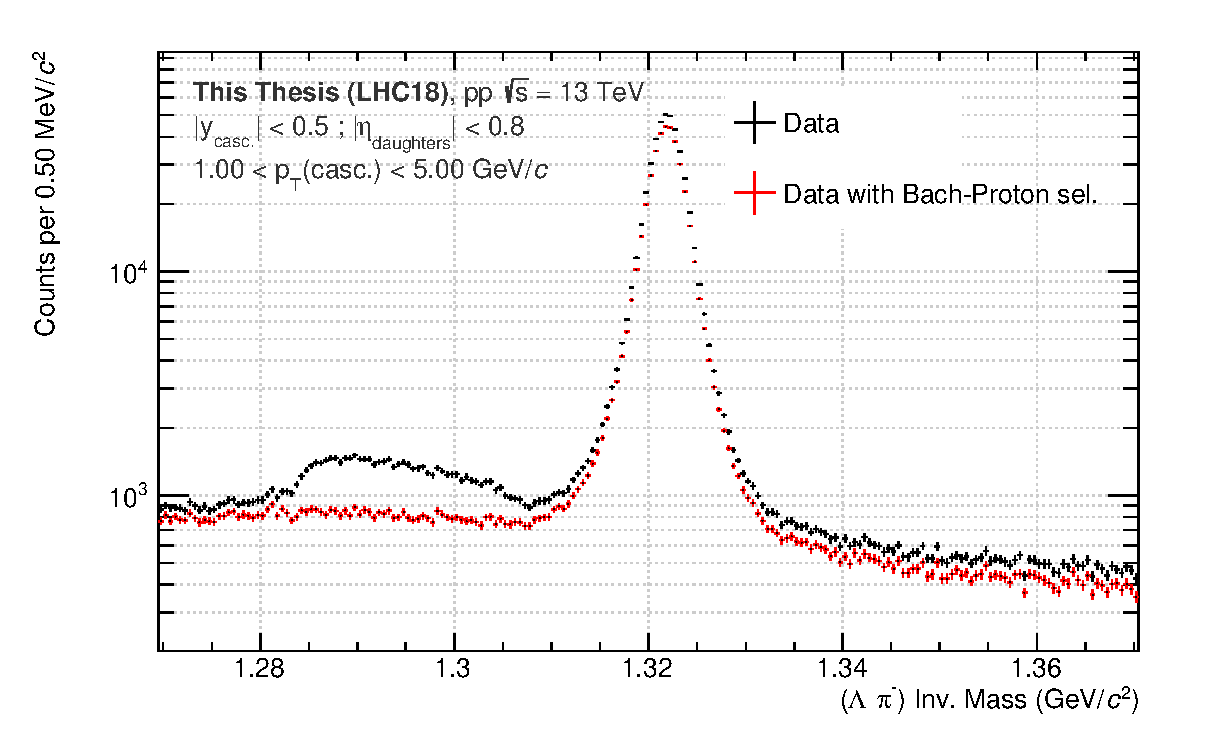
\includegraphics[width=0.6\textwidth]{Figs/Chapter5/InvMassXiMinus_WrongPA.eps}
	\label{fig:XiMinusWrongPA}
}
\subfigure[]
{
	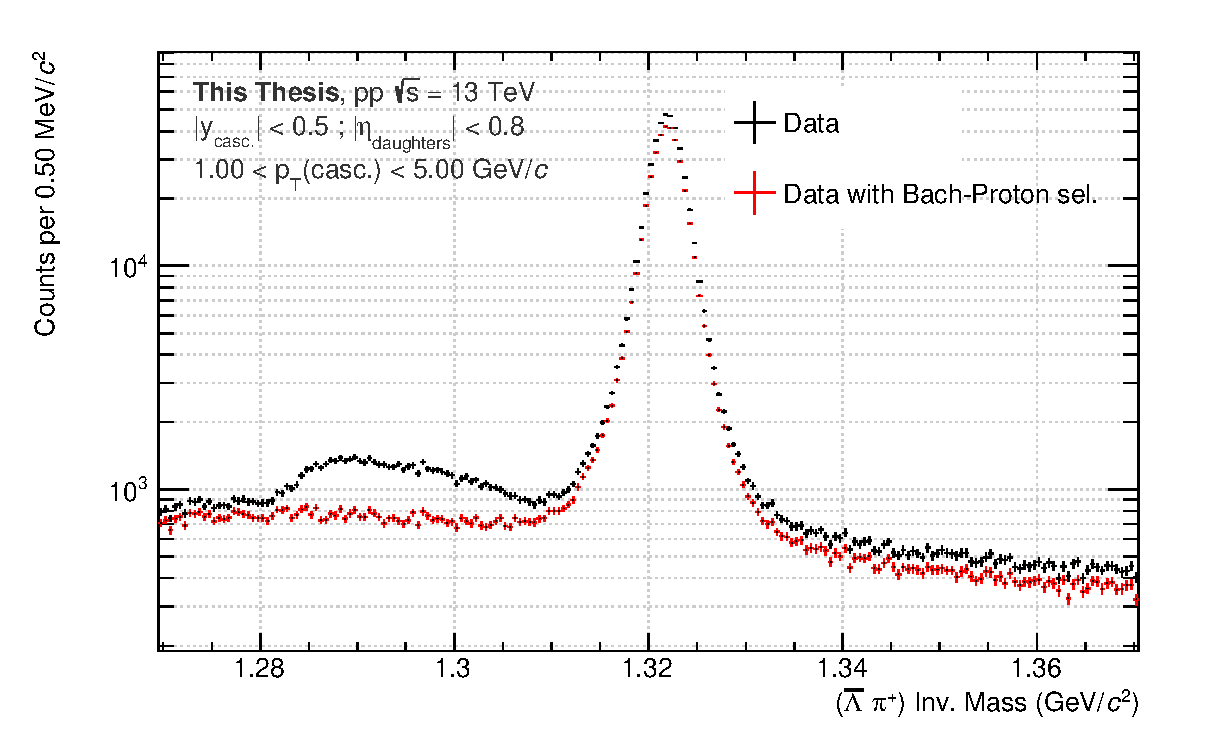
\includegraphics[width=0.6\textwidth]{Figs/Chapter5/InvMassXiPlus_WrongPA.eps}
	\label{fig:XiPlusWrongPA}
}
\hspace*{-1.5cm}	
\subfigure[]
{
	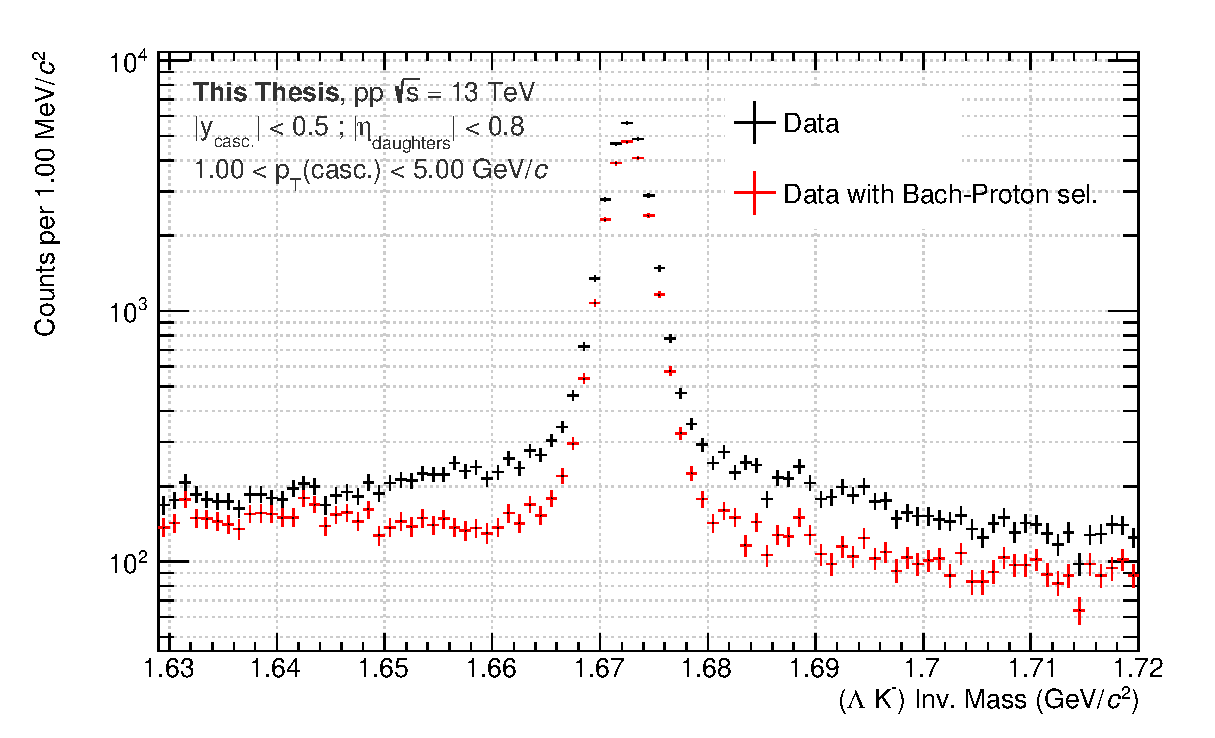
\includegraphics[width=0.6\textwidth]{Figs/Chapter5/InvMassOmegaMinus_WrongPA.eps}
	\label{fig:OmegaMinusWrongPA}
}
\subfigure[]
{
	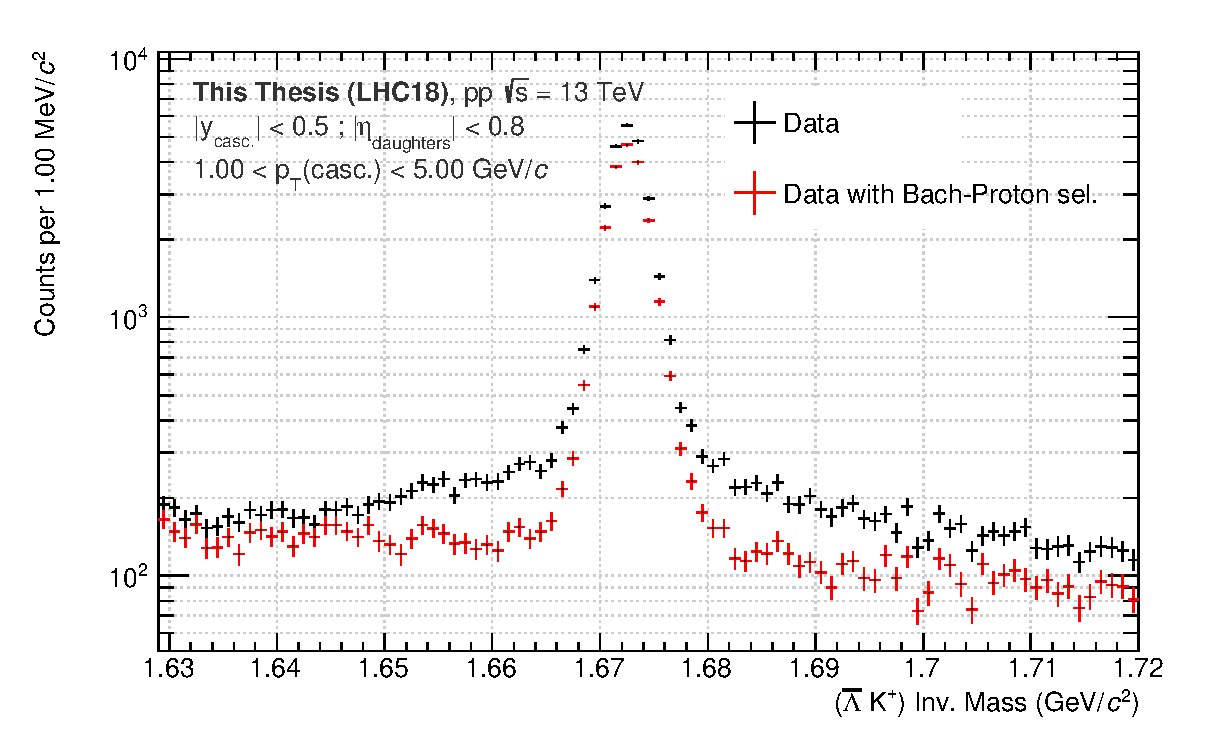
\includegraphics[width=0.6\textwidth]{Figs/Chapter5/InvMassOmegaPlus_WrongPA.eps}
	\label{fig:OmegaPlusWrongPA}
}	
	\caption{Invariant mass distribution of \rmXiM (a), \rmAxiP (b), \rmOmegaM (c) and \rmAomegaP (d) in pp at \sqrtS = 13 \tev. These have been obtained using the cuts in \tab\ref{tab:CascadeSelections} (red markers), and also without the bachelor-proton pointing angle selection (black markers). This comparison shows the latter selection manages to remove a structure in the invariant mass distribution while preserving the population under the peak. Notice the log-scale on the y-axis, that puts into perspective the signal and background levels.}
	\label{fig:WrongPA}
\end{figure}

\begin{figure}[t]
%\centering
\hspace*{-2.cm}
\subfigure[]
{
	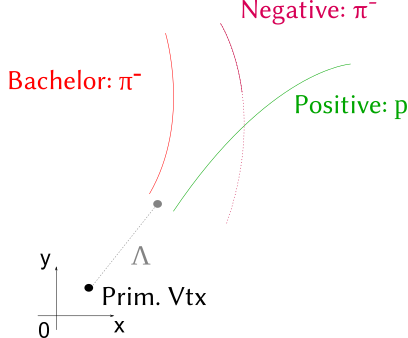
\includegraphics[width=0.32\textwidth]{Figs/Chapter5/WrongV0.png}
	\label{fig:WrongV0}
}
\subfigure[]
{
	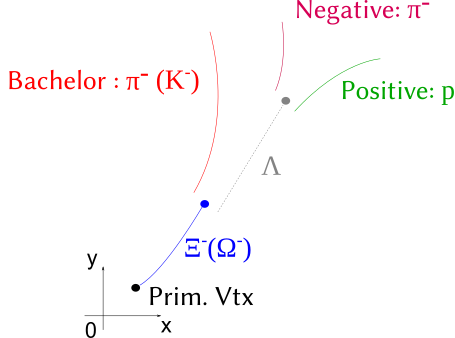
\includegraphics[width=0.32\textwidth]{Figs/Chapter5/TrueV0.png}
	\label{fig:TrueV0}
}
\subfigure[]
{
	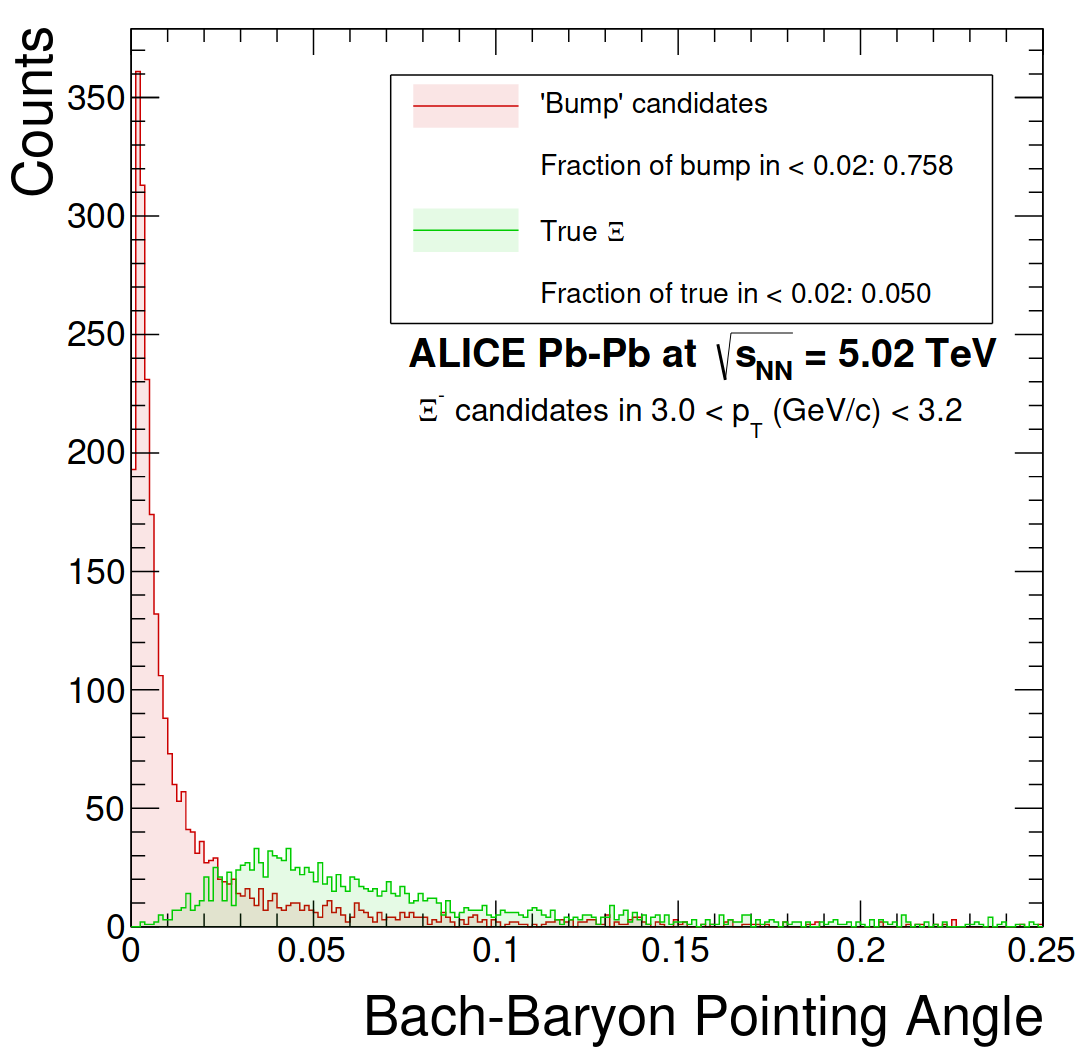
\includegraphics[width=0.4\textwidth]{Figs/Chapter5/WrongPACut.png}
	\label{fig:WrongPACut}
}
	\caption{Invariant mass distribution of \rmXiM (a), \rmAxiP (b), \rmOmegaM (c) and \rmAomegaP (d) in pp at \sqrtS = 13 \tev. These have been obtained using the cuts in \tab\ref{tab:CascadeSelections} (red markers), except for the bachelor-proton pointing angle selection in black. This comparison shows the latter selection manages to remove a structure in the invariant mass distribution while preserving the population under the peak.}
	\label{fig:WrongTopology}
\end{figure}

\subsection{Mass measurement}
\label{subsec:MassExtraction}

\subsubsection{Principles of mass extraction}
\label{subsubsec:PrinciplesOfMassExtraction}

Out of all the candidates passing the above selection criteria, there contain true V0s/cascades -- depending on the particle of interest -- and background candidates. Taken individually, they are undistinguisable. The separation of these two can only be achieved statistically, based on the analysis of the invariant mass spectrum.

The invariant mass of each candidate is calculated, as explained in \Sec\ref{subsubsec:CascadeFormation} and \Sec\ref{subsubsec:InvariantMassSelection}, and sorted according to their electric charge in order to separate the particles from the anti-particles. The V0s being electrically neutral, they follow a different approach: since the \rmKzeroS decays into two particles of the same nature --- a \rmPiPlus and a \rmPiMinus ---, it is hopeless to try separating particles and anti-particles. This is not the case of \rmLambda and \rmAlambda, though. However, it may happen that the same V0 candidate passes the particle and anti-particle selections in \tab\ref{tab:V0Selections}. To avoid such double-counting, each candidate needs to go through the \rmLambda selections first. If it satisfies all conditions, it is labeled as \rmLambda and we move to the next candidate. Otherwise, it is checked against the requirements for a \rmAlambda baryon.

On one hand, most of the background candidates originate from a random association of two or three tracks. Those tracks being uncorrelated, the corresponding invariant mass spectrum should be flat or decreasing with the invariant mass value. On the other hand, the invariant mass of true V0s/cascades should be close to the tabulated mass \mPDG, such that there emerges an overpopulated region taking the shape of a peak. The \figs\ref{fig:InvMassCascades} show the invariant mass spectra of \rmXi and \rmOmega.  One can see that the signal for each species sits on top of a small background.\\

To isolate the signal from the background, a fit of the invariant mass spectra is performed using a sum of two functions: one for modeling the signal peak, the other for describing the background. Several functions can be considered, as discussed in \Sec\ref{subsubsec:SignalShape}. In \figs\ref{fig:InvMassCascades}, the peak is represented by a triple Gaussian \cite{atlascollaborationKshortLambdaProduction2012} and the background by an exponential function. Whatever the choosen functions are, the fitting procedure is performed with the maximum (log-)likelyhood method.

If the procedure manages to converge, this fit allows to measure the mass of the considered particle: it corresponds to the centre of the invariant mass peak, given by the position of the maximum of the signal function denoted as $\mu$. The width of the peak -- the parameter $\sigma$ -- provides an estimation of the experimental resolution on the mass. The uncertainties on both quantities come from the errors returned by the fitting procedure.

From these parameters, two regions of interest can be delimited:
\begin{itemize}
\item[$\bullet$] the peak region, containing all the signal\footnote{More precisely, considering the definition of the peak region in this analysis, it should contain approximately 99.99995\% (\ie a $5 \sigma$ significance level) of the true V0s/cascades measured.} and some background, is defined within $\left[ \mu - 5 \sigma ; \mu + 5 \sigma \right]$;
\item[$\bullet$] the side-bands region, solely constituted of background, consists in two bands of the same width\footnote{As a side note: the two side-bands do not need to be of the same size, but it avoids dealing with a scaling factor when comparing their total area to the one in the peak region. Most often, they have different widths because of an asymmetry in the invariant mass distribution, such as the structure reported in \Sec\ref{subsubsec:InvMassStructure} \cite{alicecollaborationProductionLightflavorHadrons2020}.}, surrounding the peak region and covering the range $\left[ \mu - 12 \sigma ; \mu - 7 \sigma \right] \bigcup \left[ \mu + 7 \sigma ; \mu + 12 \sigma \right]$.
\end{itemize}
Hence, the amount of raw signal and background can be evaluated. The peak ($S+B$) and background ($B$) populations are estimated by counting the
number of candidates in their respective regions. The raw signal ($S$) in the peak region is obtained by subtracting the background from the peak population, that is $S = (S+B) - B$.

\begin{figure}[p]
%\centering
\hspace*{-1.5cm}
\subfigure[]{
	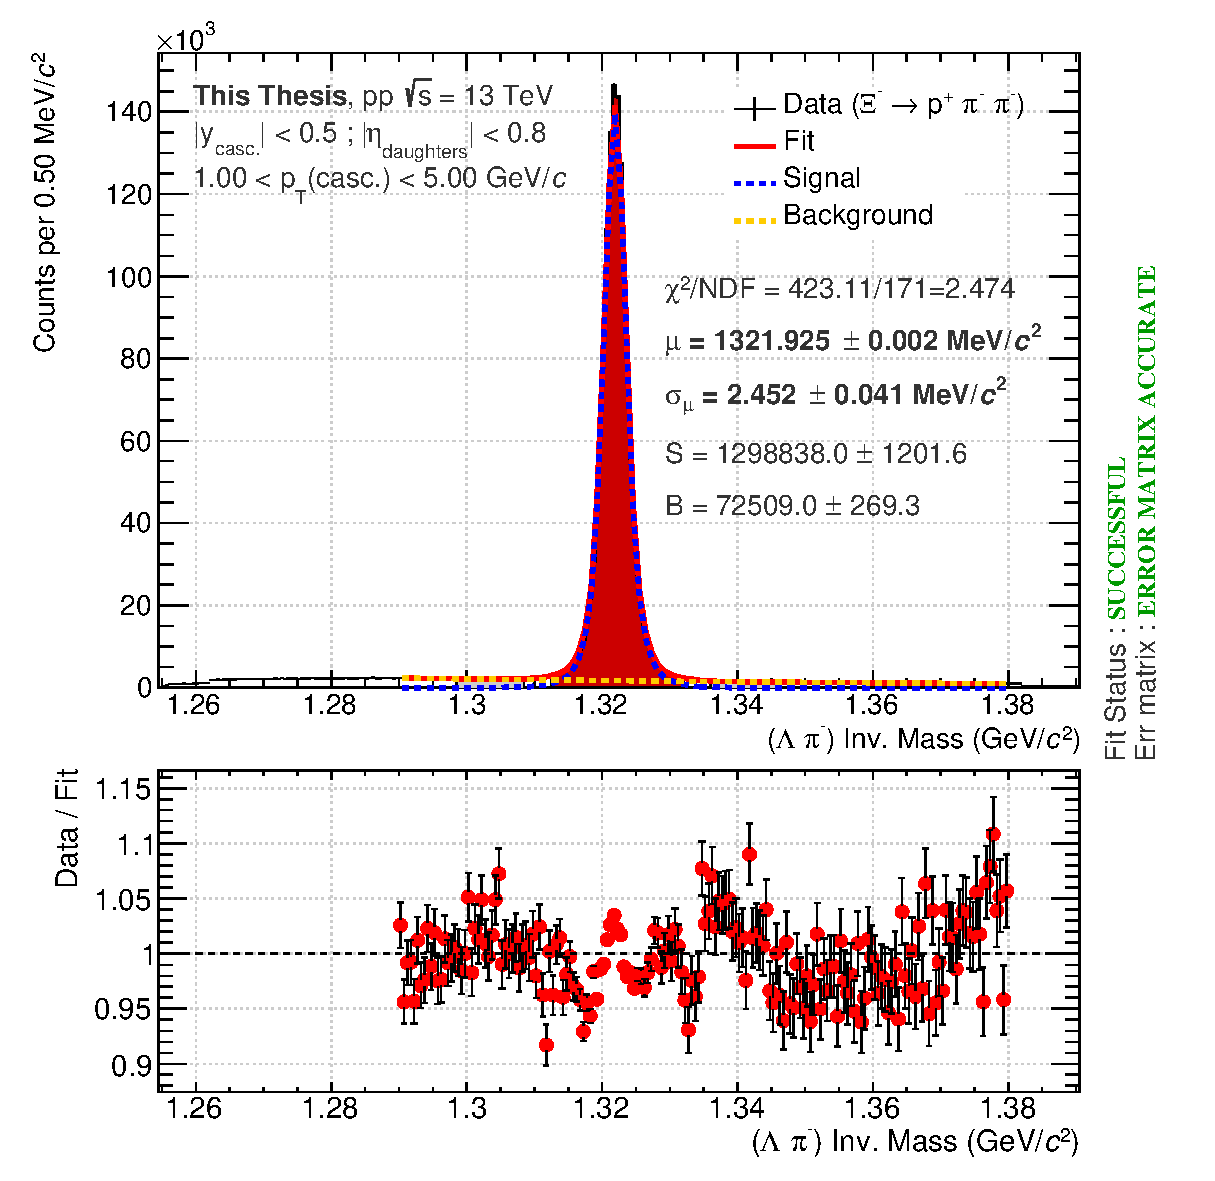
\includegraphics[width=0.6\textwidth]{Figs/Chapter5/InvMassXiMinus.eps}
	\label{fig:XiMinus_ModGaussian}
} 
\subfigure[]{
	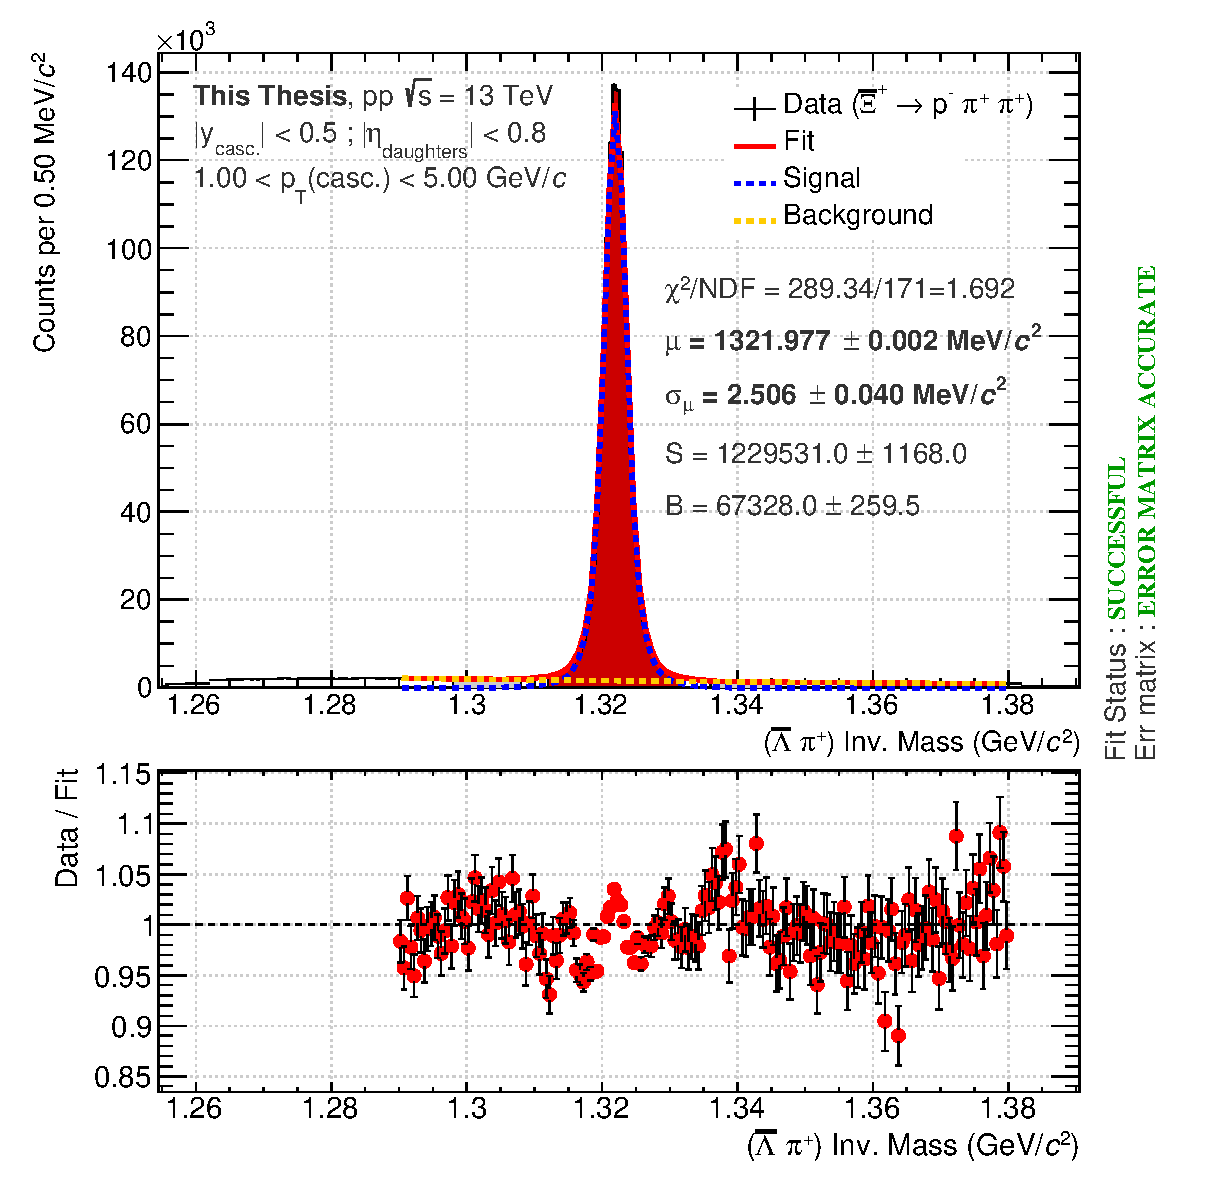
\includegraphics[width=0.6\textwidth]{Figs/Chapter5/InvMassXiPlus.eps}
	\label{fig:XiPlus_ModGaussian}
} 
\hspace*{-1.5cm}
\subfigure[]{
	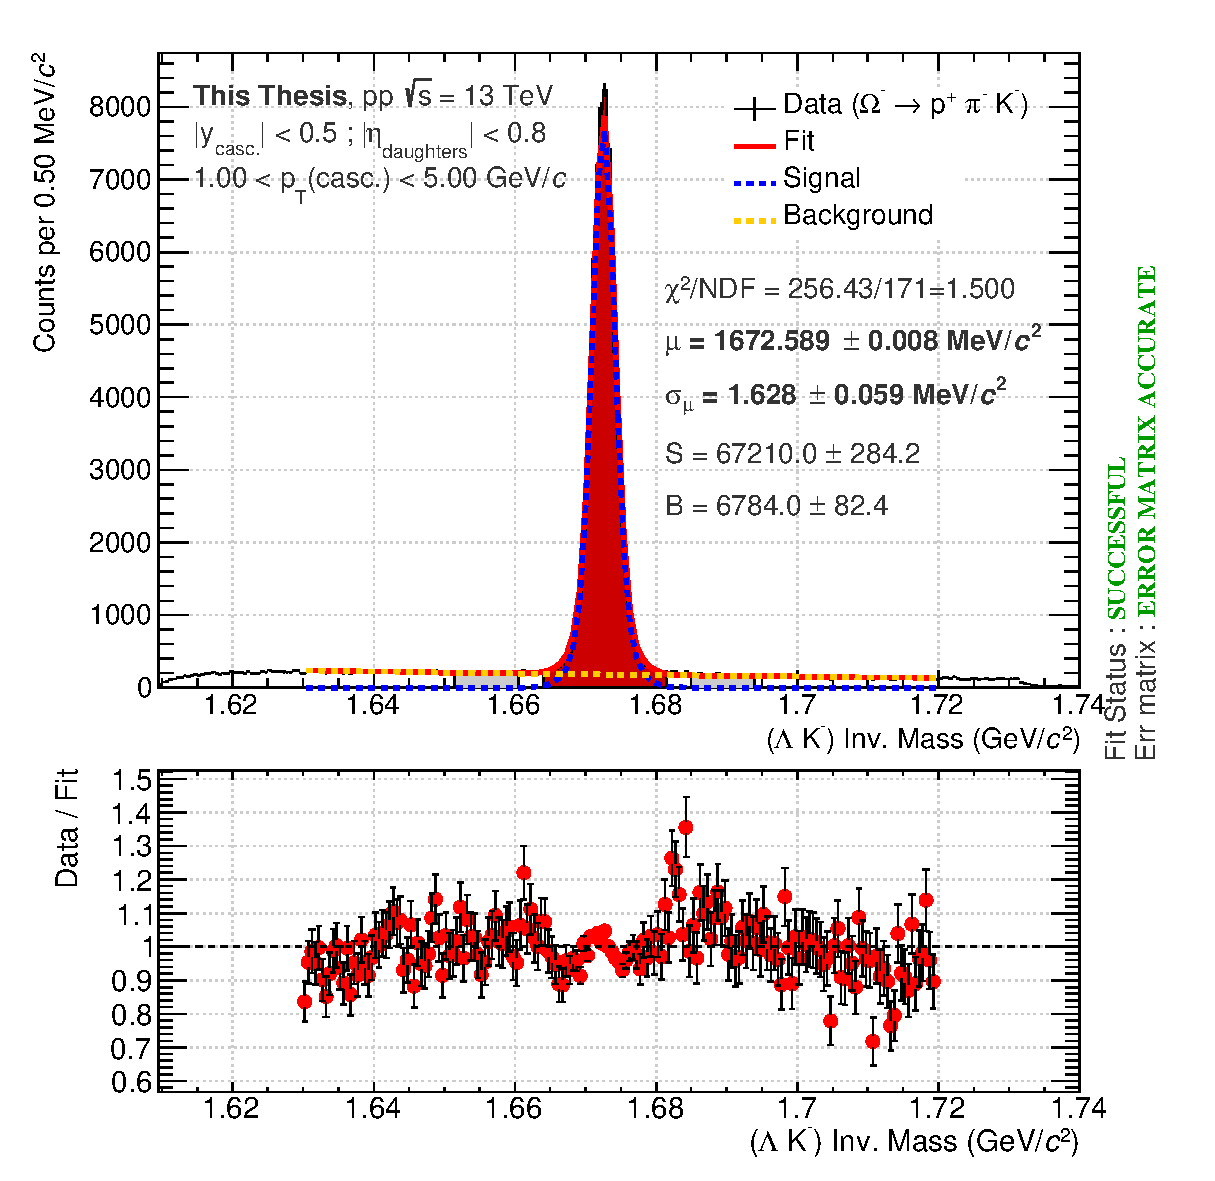
\includegraphics[width=0.6\textwidth]{Figs/Chapter5/InvMassOmegaMinus.eps}
	\label{fig:OmegaMinus_ModGaussian}
} 
\subfigure[]{
	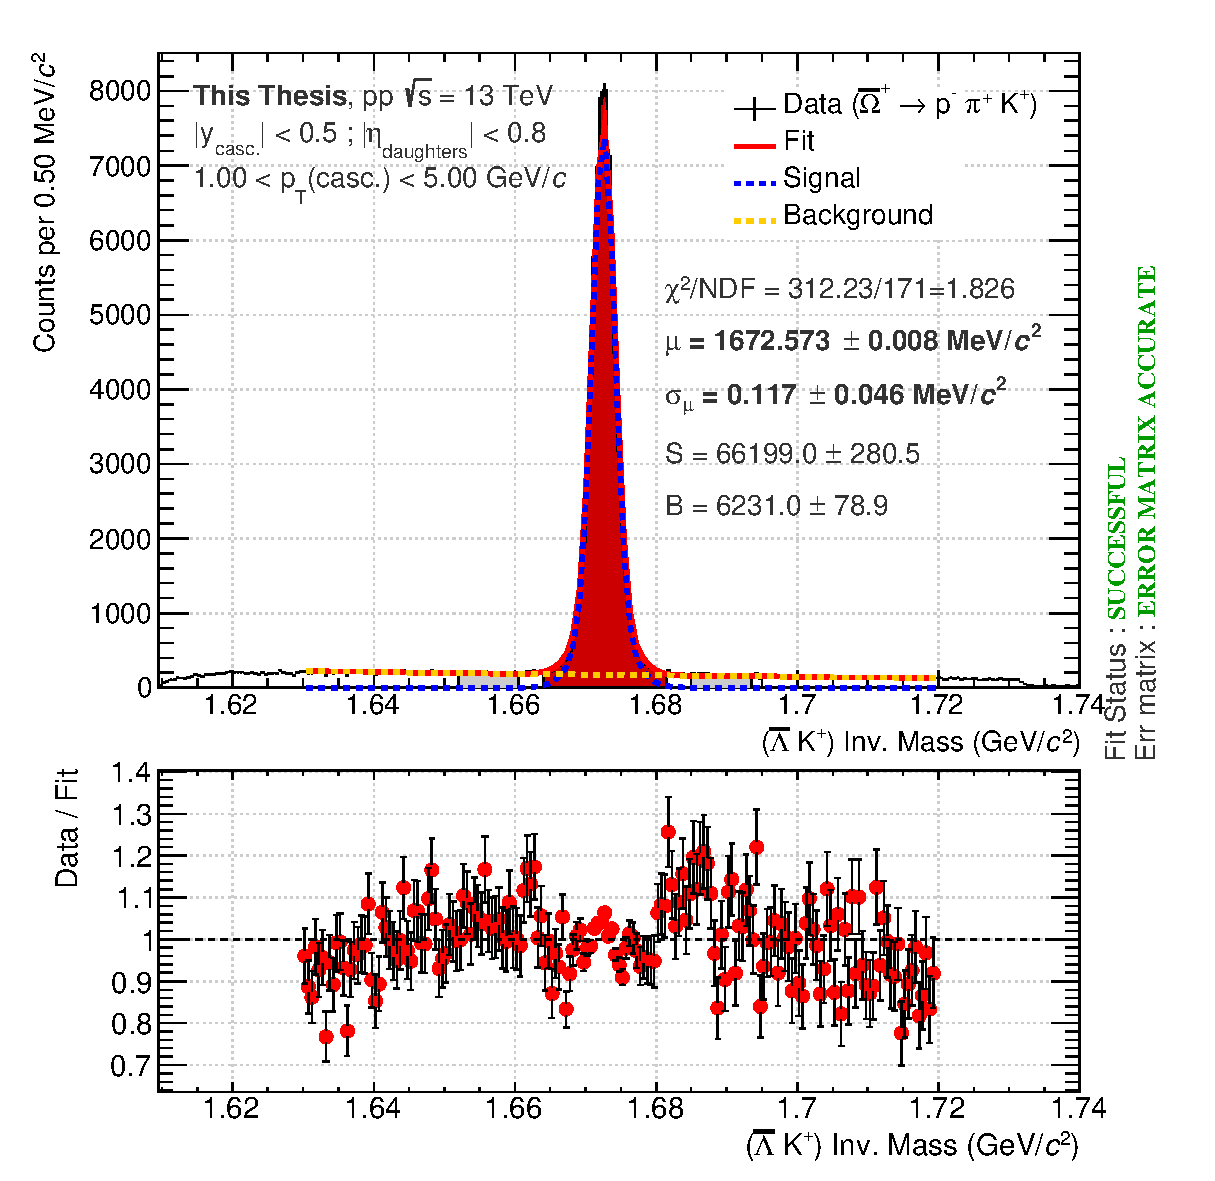
\includegraphics[width=0.6\textwidth]{Figs/Chapter5/InvMassOmegaPlus.eps}
	\label{fig:OmegaPlus_ModGaussian}
}  
\caption{Invariant mass distribution of \rmXiM (a), \rmAxiP (b), \rmOmegaM (c) and \rmAomegaP (d) hyperons in pp collisions at \sqrtS = 13 \tev. Here, the peak is modeled by a triple Gaussian, and the background by an exponential function. Each distribution comes with an additional panel representing the consistency between the data and the fit model, in the form of a ratio per invariant mass bin. The error bars encompasses the uncertainties on both quantities.}
	\label{fig:InvMassCascades}
\end{figure}

In \figs\ref{fig:InvMassCascades}, all the fit are of reasonably good quality\footnote{One may argue that, in the case of the \rmXiM, the reduced $\chi^{2}$  is relatively high. However, the comparison of the bottom panels of the \rmXiM and \rmAxiP allows to conclude that it certainly comes from a slightly worst description of the background.}. The bottom panels show that the data-model discrepancy does not exceed 5\% for the most precise points, \ie those in the peak region. The mass peak sits on a small background: 1 298 838 $\pm$ 1202 \rmXiM (1 229 531 $\pm$ 1168 \rmAxiP) and 67 210 $\pm$ 285 \rmOmegaM (66 199 $\pm$ 281 \rmAomegaP) were reconstructed with purities above 90\%, as shown in \tab\ref{tab:FitQuantities}.

\begin{table}[h]
    \centering
    \begin{tabular}{b{5.35cm}@{\hspace{1cm}} b{2cm}@{\hspace{0.5cm}} b{2cm}@{\hspace{0.5cm}} b{1.5cm}@{\hspace{0.5cm}} b{1.5cm}@{\hspace{0.1cm}}}
    \noalign{\smallskip}\hline\noalign{\smallskip}
	\bf Particle & \rmXiM & \rmAxiP & \rmOmegaM & \rmAomegaP \\	
    \noalign{\smallskip}\hline \noalign{\smallskip}
    Reduced $\chi^2$ & 2.474 & 1.692 & 1.500 & 1.826\\
    	Raw signal, $S$ &  1 298 838 & 1 229 531 & 67 210 & 66 199\\
    	Background, $B$ & 75209 & 67 328 & 6784 & 6231 \\
    	$S/B$ & 17.3 & 16.4 & 9.91 & 10.63 \\
    	Purity, $S/(S+B)$ & 94.5\% & 94.2\% & 90.8\% & 91.4\% \\
    Signal significance, $S/\sqrt{S+B}$ & 1108 & 1076 & 247 & 246 \\
    \noalign{\smallskip}\hline\noalign{\smallskip}
    \end{tabular}
    \caption{Results from the fit of the invariant mass distributions in \fig\ref{fig:InvMassCascades} concerning the overall samples of \rmXiM, \rmAxiP, \rmOmegaM and \rmAomegaP. Therefore, this table reports the reduced $\chi^{2}$, raw signal, background, ratio $S/B$, purity and signal significance.}\label{tab:FitQuantities}
\end{table}

\subsubsection{Shape of the peak functions}
\label{subsubsec:SignalShape}

Since the mass extraction depends on the peak description, it is crucial to identify functional forms that reproduce accurately its shape. Different functions have been studied in MC simulations, based solely on true V0/cascade candidates. Thus, the invariant mass spectra contains no background candidates and follows approximately a quasi-Gaussian distribution centred on the injected mass, which usually corresponds to the PDG mass value. The objective here is to define a list of functions, that describe correctly the shape of the invariant mass peak and are characterised by a reasonably good reduced $\chi^{2}$. Two types of functional forms are considered: symmetric and asymmetric functions. 

\paragraph{Symmetric function:} Due to the detector smearing, the core of the invariant mass distribution exhibits a quasi-Gaussian shape; in that respect, one may favour symmetric functions. The tails of the distribution, however, are usually not Gaussian-like, and thus not well described by this class of functions. This is due to the contribution of particles with different transverse momentum; as the \pT resolution varies with the transverse momentum and relates to the width of the invariant mass peak, the measured distribution consists in fact in an infinite sum of invariant mass distribution, each with a different width. Always with the aim of employing an symmetric function, the solution thus consists to take an infinite sum of Gaussian with a common mean\footnote{A more unusual approach would be to consider an infinite sum of Gaussian, each with a different mean. This would be relevant if the mass measurement is biased, in such a way that mass changes with momentum for example. In such case, a non-trivial question arises as of what value to take as a final mass measurement. As of today, there is still no clear answer.}. In the present analysis, it has been observed that three Gaussians (\eq\ref{eq:Gaus}) already offer a reasonably good fit quality. Another option is to resort to slightly modified versions of a Gaussian, such that it provides a better description of the tails of the distribution (\eq\ref{eq:ModifiedGaus}).

\begin{itemize}
\item[$\bullet$] \textbf{Triple Gaussian}:
	\begin{equation}
	\dNdX{\mInv[]} = A_{1} \cdot \exp \left[ - \dfrac{ (\mInv[] - \mu )^2}{ 2 \sigma_{1}^2} \right] + A_{2} \cdot \exp \left[ - \dfrac{ (\mInv[] - \mu )^2}{ 2 \sigma_{2}^2} \right] + A_{3} \cdot \exp \left[ - \dfrac{ (\mInv[] - \mu )^2}{ 2 \sigma_{3}^2} \right]
	\label{eq:Gaus}
	\end{equation}
	with $A_{1}$, $A_{2}$, $A_{3}$ the amplitudes of the first, second and third Gaussian, $\mu$ the common mean value, and $\sigma_{1}$, $\sigma_{2}$, $\sigma_{3}$ the width of the first, second and third Gaussian\footnote{In case of a fit with a triple Gaussian function, it is the weighted width that is considered for the definition of the peak and side-bands regions. The weighting factors for $\sigma_{1}$, $\sigma_{2}$, $\sigma_{3}$ are determined based on the relative contribution of each Gaussian in the fit, \ie $\sigma^{2} = \frac{A_{1}}{A_{1}+A_{2}+A_{3}} \sigma_{1}^{2} + \frac{A_{2}}{A_{1}+A_{2}+A_{3}} \sigma_{2}^{2} + \frac{A_{3}}{A_{1}+A_{2}+A_{3}} \sigma_{3}^{2}$}.
%	
%\item \textbf{Double Gaussian} : it consists in a sum of two Gaussian functions with different parameters but the mean value which is common.
%	\begin{equation}
%	\dNXdX{\rmXiPM(\rmOmegaPM)}{\mInvIdx{\rmLambdaPM \piPlusMinus (\rmLambdaPM \Kplusmin)}} = A_{1} \cdot \exp \left[ - \dfrac{ (\mInvIdx{\rmLambdaPM \piPlusMinus (\rmLambdaPM \Kplusmin)} - \mu )^2}{ 2 \sigma_{1}^2} \right] + A_{2} \cdot \exp \left[ - \dfrac{ (\mInvIdx{\rmLambdaPM \piPlusMinus (\rmLambdaPM \Kplusmin)} - \mu )^2}{ 2 \sigma_{2}^2} \right]
%	\end{equation}\label{eq:DoubleGaus}
%	where $A_1$ and $A_2$ are the respective amplitudes of the two Gaussian, $\mu$ corresponds to the center of the peak (common for the two Gaussian), and their widths are denoted as $\sigma_1$ and $\sigma_2$.
%	
\item[$\bullet$] \textbf{Modified Gaussian} \cite{atlascollaborationKshortLambdaProduction2012}:
	\begin{equation}
	\dNdX{\mInv} = A \cdot \exp \left[ - \frac{1}{2} u^{1 + \frac{1}{1+ 0.5 u}} \right] \quad ; \quad  u = \left\rvert \frac{\mInv - \mu }{\sigma} \right\rvert
	\end{equation}\label{eq:ModifiedGaus}
	with $A$ the normalization, $\mu$ the mean, and $\sigma$ the width.\\
	
\end{itemize}

\paragraph{Asymmetric function:} Previous functions are all different flavours of Gaussian, and so are all symmetric. However, this is not necessarily the case for the tails of the invariant mass distribution. In such case, an asymmetric function seems more suited for describing the peak. Among those appears the Bukin function  \cite{bukinFittingFunctionAsymmetric2007}\cite{nielPreciseMeasurementsCharmed2021}, that is modified Novosibirsk distribution, constructed from the convolution of a Gaussian and an exponential distributions. It is typically used to fit the invariant mass of \rmJpsi.

\begin{itemize}
\item[$\bullet$] \textbf{Bukin}:
	\begin{equation}
	\dNdX{\mInv} = 
		\begin{cases}
	      A \cdot \exp \left[ \rho_{\rm L} \frac{(u-x_{\rm L})^2}{(\mu-x_{\rm L})^2} - \ln(2) + 4 \cdot \ln(2)  \frac{(u-x_{\rm L})}{2 \sigma \sqrt{ 2  \ln 2 }} \cdot  \frac{\xi}{\sqrt{\xi^2+1} + \xi}  \frac{\sqrt{\xi^2+1}}{(\sqrt{\xi^2+1}-\xi)^2} \right], \qquad u\leq x_{\rm L} \\
	      \\
	      A \cdot \exp \left[ -\ln(2) \cdot \left( \frac{ \ln(1 + 4 \xi \sqrt{\xi^2+1} \frac{u - \mu}{2 \sigma \sqrt{2 \ln 2}}) }{ \ln( 1 + 2 \xi (\xi - \sqrt{\xi^2+1})) } \right)^2 \right], \qquad  x_{\rm L} < u < x_{\rm R} \\
	      \\
	      A \cdot \exp \left[ \rho_{\rm R} \frac{(u-x_{\rm R})^2}{(\mu-x_{\rm R})^2} - \ln(2) + 4 \cdot \ln(2) \frac{(u-x_{\rm R})}{2 \sigma \sqrt{ 2  \ln 2 }} \cdot  \frac{\xi}{\sqrt{\xi^2+1} + \xi} \frac{\sqrt{\xi^2+1}}{(\sqrt{\xi^2+1}-\xi)^2} \right], \qquad u \geq x_{\rm R} 
	     \end{cases}
	\end{equation}\label{eq:Bukin}
	with 
	\begin{equation}
		x_{\rm L, R} = \mu + \sigma \sqrt{ 2 \ln 2 } \left( \frac{ \xi}{ \sqrt{\xi^2 + 1 } } \mp 1 \right)
	\end{equation}
	where $u$ coincides with \mInv, $A$ is the normalization parameter, $\mu$ and $\sigma$ are the mean and the width of the peak, $\xi$ is an asymmetry parameter, $\rho_{\rm L}$ and $\rho_{R}$ are left and right exponential tail coefficients \cite{verkerkeRooFitUsersManual2008}.
	
\item[$\bullet$] \textbf{Double-sided crystal ball} \cite{atlascollaborationSearchResonancesDiphoton2016}:
	\begin{equation}
	\dNdX{\mInv} = 
		\begin{cases}
	      A \cdot \left(\frac{n_{\rm L}}{\alpha_{\rm L} (n_{\rm L} - \alpha_{\rm L}^{2} - u \alpha_{\rm L})}\right)^{n_{L}} \exp \left[ -0.5  \alpha_{\rm L}^{2} \right] , \qquad u < -\alpha_{\rm L} \\
	      \\
	      A \cdot \exp \left[ -0.5 u^{2} \right], \qquad  -\alpha_{\rm L} \leq u \leq \alpha_{\rm R} \\
	      \\
	      A \cdot \left(\frac{n_{\rm R}}{\alpha_{\rm R} (n_{\rm R} - \alpha_{\rm R}^{2} + u \alpha_{\rm R})}\right)^{n_{R}} \exp \left[ -0.5  \alpha_{\rm R}^{2} \right] , \qquad u < \alpha_{\rm R} 
	     \end{cases}
	\end{equation}\label{eq:DoubleSidedCrystalBallFunction}
	with $u$ equals $\left(\mInv - \mu\right)/\sigma_{L}$ for $\mInv - \mu < 0$ and $\left(\mInv - \mu\right)/\sigma_{R}$ for $\mInv - \mu > 0$, $A$ is the normalization parameter, $\mu$ is the peak position, $\sigma_{\rm L}$ and $\sigma_{\rm R}$ parametrise the position where the peak starts to follow a power law towards the low and high mass values respectively, of exponents $n_{\rm L}$ and $n_{\rm R}$.

\end{itemize}

To each particle should be associated, at least, two functional forms for the modelisation of the peak: a symmetric and an asymmetric functions. Therefore, after several tests, it turns out that the functions offering the best description of the invariant mass peak are the triple Gaussian and the Bukin. In addition, the fit tends to converge more easily with the latter function than with the double-sided crystal ball function. Consequently, only these two functions will be considered in the following.

\subsubsection{Shape of the background functions}
\label{subsubsec:BackgroundShape}

The origin of the data sample purity has to be found in the (very) tight cut on the cosine of pointing angle of the cascade candidate in \tab\ref{tab:CascadeSelections}. As a matter of fact, this selection has been tuned to reach such level of purity. Contrarily to the peak shape, the form of background is \textit{a priori} lesser known. For that reason, it is essential to control the level of background, and most particularly its profile, such that it can be modeled by one of the expected functional form.

For the background, different functional forms are considered :

\begin{itemize}
\item \textbf{Constant}: one may suspect the combinatorial background to be \textit{a priori} unstructured. In such case, it should follow a uniform distribution, and thus can be approximated by a constant function.
\item \textbf{Linear}: The previous description can be refined by considering that the number of tracks decreases with momentum. Consequently, the misassociation of low momentum tracks should dominate the combinatorial background at the low invariant mass values, whereas the high values originate from tracks with higher momentum. Hence, the background reduces with the invariant mass value. This decrease may be parametrised, at first order, by a linear function.
\item \textbf{Exponential}: Alternatively, the background can also be decreased by an exponential function.
\item \textbf{Second order polynomial}: In case the background turns out not to be purely combinatorial, but has a physics origin like, for instance particles produced from the interaction with the detector material. In such scenario, the background may have a specific structure, that needs to be described by more parameters than in the above functions. To that end, a second order polynomial is also considered for modeling the background.
\end{itemize}

Since the exploited simulations contain only pure samples of strange hadrons, the study of the most appropriate background shapes for each of the considered particles has to be performed on the data\footnote{As a matter of fact, even if the exploited MC simulations would contain some background, there is no guarantee that they provide the same background as in the real data.}. To obtain an invariant mass distribution consisting only of background candidates, the peak is removed by cutting out all the entries falling in an invariant mass region of $\mPDG \pm 10$ \mmass. The obtained invariant mass spectra is then fitted with each of the above functional forms, in order to identify those describing accurately the background. 

For \rmKzeroS, \rmLambda, \rmXi and \rmOmega, the best parametrisations of the background turn out to be a linear and an exponential functions. Thereby, only these forms will be considered in the following.\\

In total, there are two functions for modeling the peak, and two functions for the description of the background. All the combinations between these two pairs of functional forms have been tested: the sum of a triple Gaussian and an exponential function offers the best description. Therefore, the latter will provide our mass measurement; the other associations of peak and background functions will be used for the study of the systematic uncertainties.


\subsubsection{Correction on the extracted mass}
\label{subsubsec:CorrectionOnTheExtractedMass}

Although the functions in \Sec\ref{subsubsec:SignalShape} describe well the invariant mass peak, the extracted mass does not agree with the PDG mass (see \tab\ref{tab:V0CascPDGMass}), as shown in \figs\ref{fig:InvMassCascades}. This seemingly bias may stem from several reasons. It can be due to the way data are processed, that might overestimate the reconstructed mass in a systematic manner. The analysis, and particularly the employed selections, may introduce a distortion in the invariant mass distribution, resulting in a different mass than the expected one. The fit procedure could also be the origin of such inconsistency; for instance, one of the tails may pre-dominate the procedure and drive the parameters in a certain direction.

Anyhow, in order to correct for any bias due to the data processing, the analysis or the fit procedure, an offset is applied on the extracted mass in simulated events such that it coincides with the injected value, which is always set to the corresponding PDG mass in our simulations. It follows that this correction is then reported on the measured mass in real data. However, such a correction assumes a good agreement between the data and MC. To ensure that, the simulation is re-weighted to match the raw \pT spectra from the data.

This re-weighting procedure starts off by extracting the raw \pT spectra in the data. Similarly to the estimation of the amount of raw signal in \Sec\ref{subsubsec:PrinciplesOfMassExtraction}, the latter is given by subtracting the \pT spectrum in the side-bands region from the one in the peak region. It is then compared to the injected transverse momentum distribution of true V0/cascade candidates; the ratio of the \pT spectra in the data and MC provides the weighting factors.


\begin{figure}[!t]
%\centering
\hspace*{-1.5cm}
\subfigure[]{
	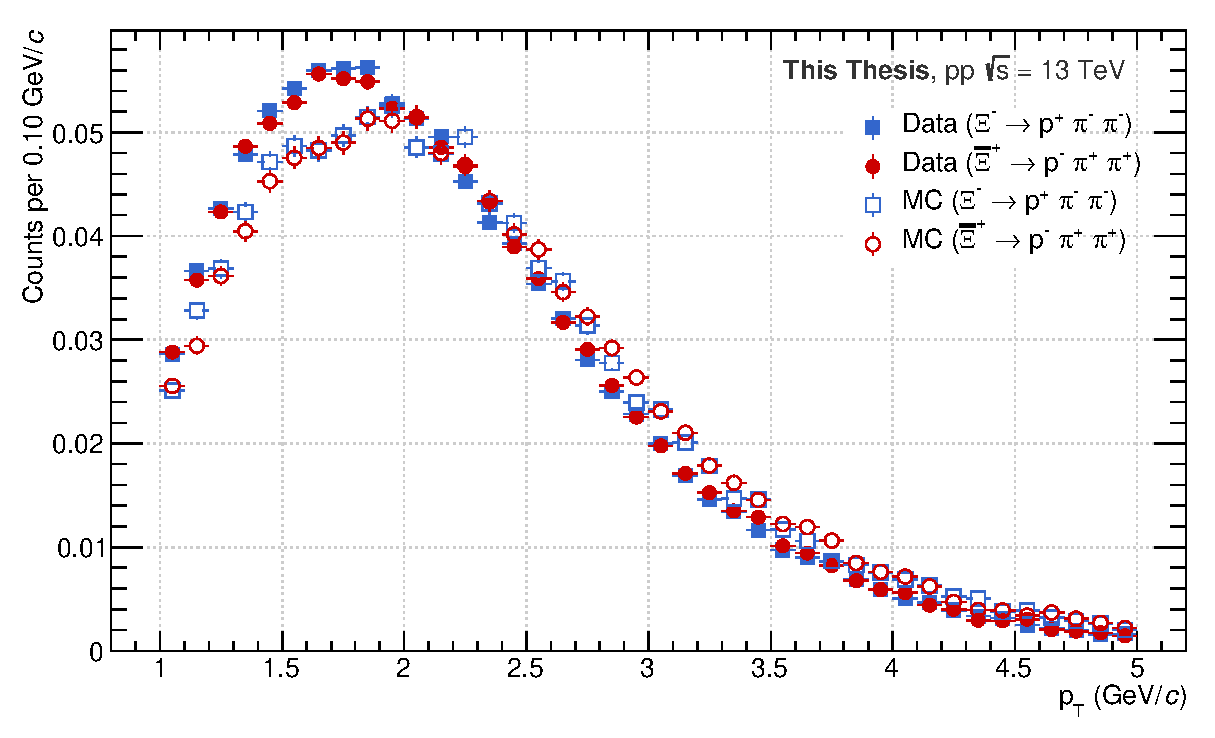
\includegraphics[width=0.6\textwidth]{Figs/Chapter5/RawPtSpectra_Xi.eps}
	\label{fig:XiMinus_ModGaussian}
} 
\subfigure[]{
	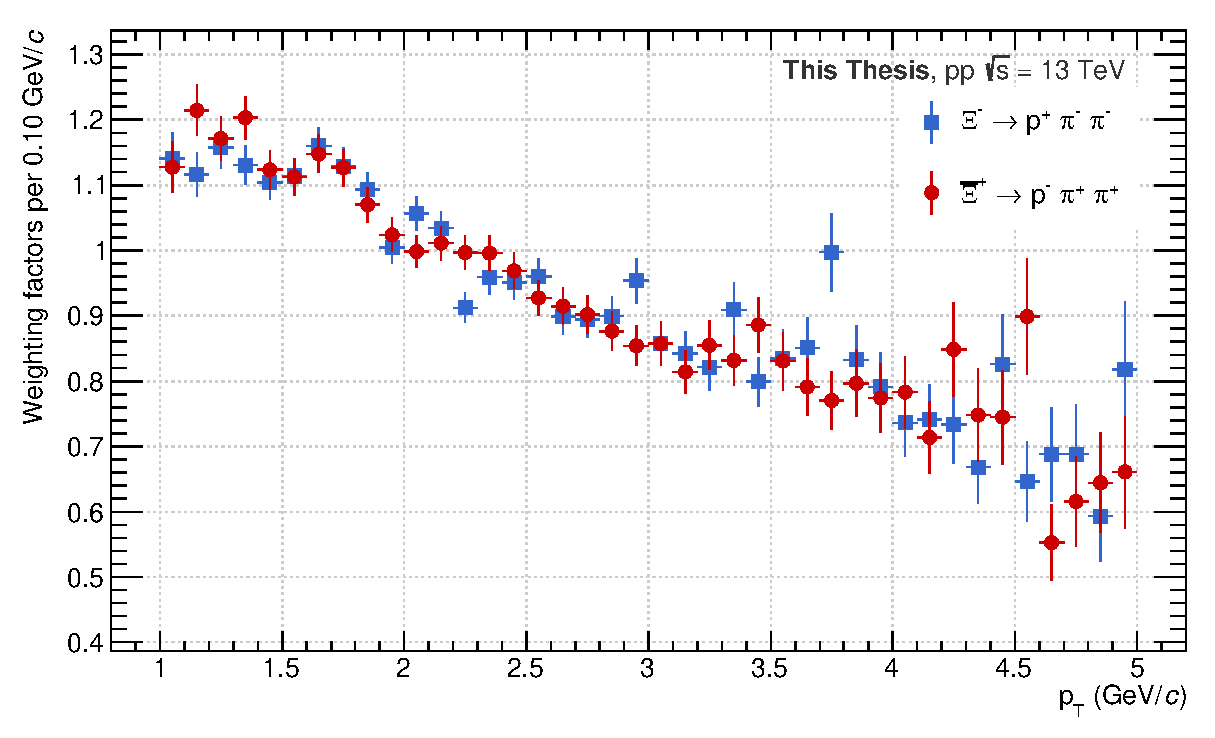
\includegraphics[width=0.6\textwidth]{Figs/Chapter5/WeightingFactors_Xi.eps}
	\label{fig:XiPlus_ModGaussian}
} 
\hspace*{-1.5cm}
\subfigure[]{
	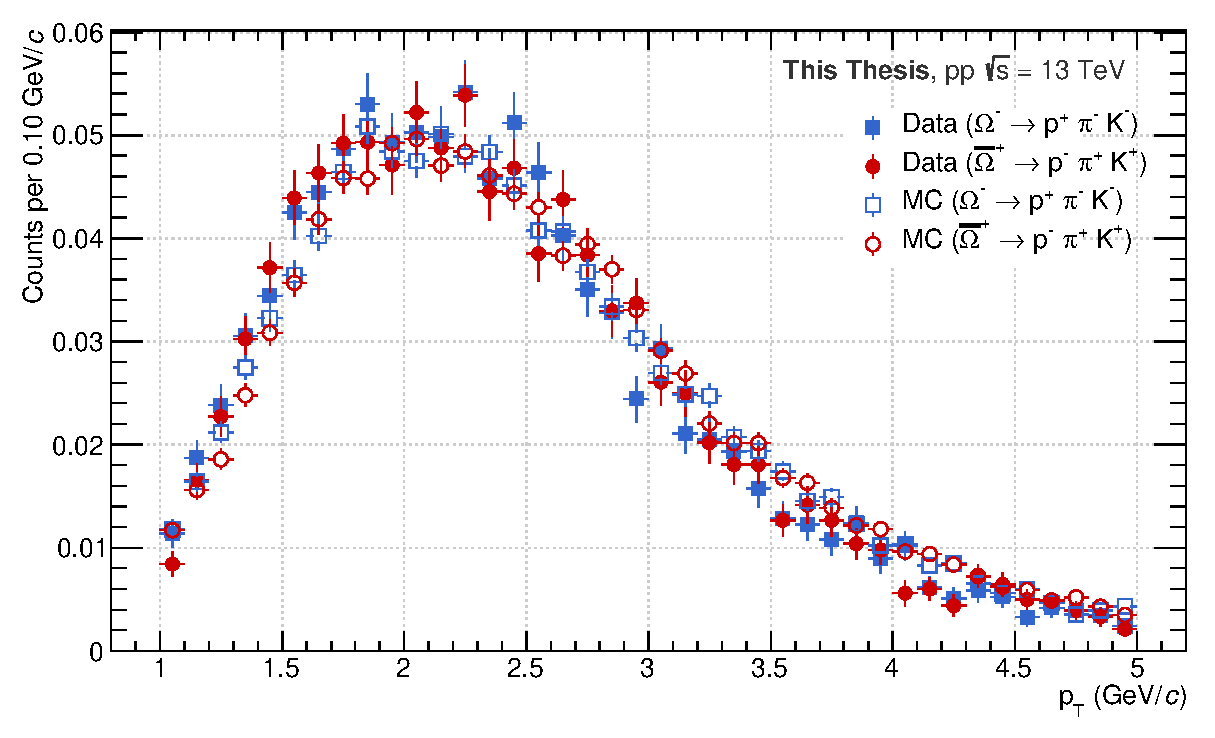
\includegraphics[width=0.6\textwidth]{Figs/Chapter5/RawPtSpectra_Omega.eps}
	\label{fig:OmegaMinus_ModGaussian}
} 
\subfigure[]{
	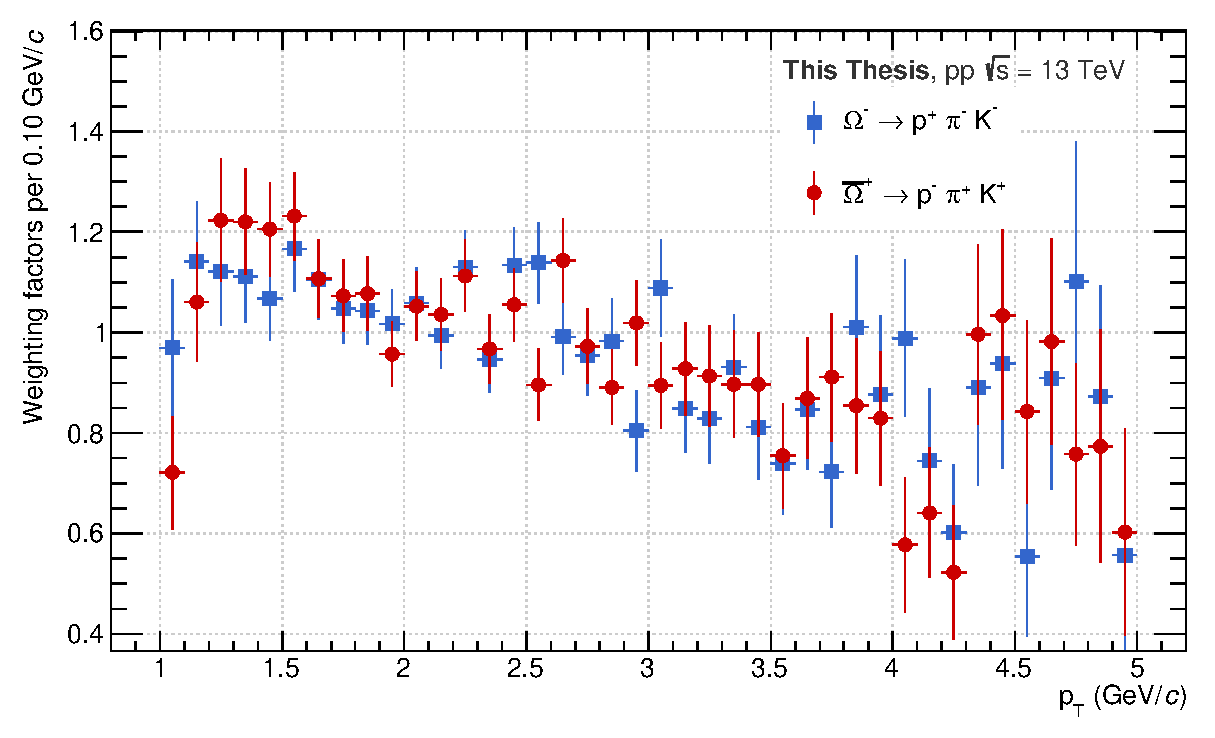
\includegraphics[width=0.6\textwidth]{Figs/Chapter5/WeightingFactors_Omega.eps}
	\label{fig:OmegaPlus_ModGaussian}
}  
\caption{On the left: raw \pT spectra of \rmXiM and \rmAxiP (a), and \rmOmegaM and \rmAomegaP (c) hyperons in the data in full marker, and in simulations in open markers. On the right: weighting factors for \rmXiPM (b) and \rmOmegaPM (d), employed to match the \pT spectra in the data and MC. The error bars encompasses only the statistical uncertainties.}
	\label{fig:PtSpectra}
\end{figure}


Once the simulated data have been re-weighted, the mass offset observed in MC with respect to the injected mass is assessed, corrected and taken into account in the mass measurement in real data. The \tab\ref{tab:MCMassOffset} presents these corrections as well as the corrected mass values, \ie those measured in real data after correction of the initial offset in MC. From these derive the (relative) mass difference between particle and anti-particle, given by
\begin{equation}
\frac{\Delta \mu}{\mu}=  2 \cdot \frac{\mu_{\textsc{part.}}-\mu_{\overline{\textsc{part.}}}}{\mu_{\textsc{part.}}+\mu_{\overline{\textsc{part.}}}}.
\label{eq:MassDifference}
\end{equation}
Its (statistical) uncertainty is obtained via propagation of the ones on the mass values, assuming there is no correlation between the particle and anti-particle measurements -- \textit{a priori} correct, since $\mu_{\textsc{part.}}$ and $\mu_{\overline{\textsc{part.}}}$ have been extracted independently\footnote{The facts that i) the particle and anti-particle do not share the same data sample (\Sec\ref{subsubsec:PrinciplesOfMassExtraction}), and ii) the fitting procedure is run separately guarantee the independence of the mass measurements.}--,
\begin{equation}
\sigma_{\Delta \mu /\mu }=  4 \cdot \sqrt{ \left(\frac{-\mu_{\overline{\textsc{part.}}}}{\left(\mu_{\textsc{part.}} + \mu_{\overline{\textsc{part.}}} \right)^{2}}\right)^{2} \sigma_{\mu_{\textsc{part.}}}^{2} + \left(\frac{\mu_{\textsc{part.}}}{\left(\mu_{\textsc{part.}} + \mu_{\overline{\textsc{part.}}} \right)^{2}}\right)^{2} \sigma_{\mu_{\overline{\textsc{part.}}}}^{2} }.
\label{eq:MassDifferenceUncertainty}
\end{equation}
The \tab\ref{tab:MCMassDiffOffset} shows mass difference for \rmXi and \rmOmega, in the data and MC, as well as the corrected value.

\begin{table}[!t]
    \centering
    \footnotesize
    \begin{tabular}{>{\raggedleft\arraybackslash}b{2.5cm}@{\hspace{0.5cm}} >{\raggedleft\arraybackslash}b{2.5cm}@{\hspace{0.5cm}} >{\raggedleft\arraybackslash}b{2.5cm}@{\hspace{0.5cm}} >{\raggedleft\arraybackslash}b{2.5cm}@{\hspace{0.5cm}} >{\raggedleft\arraybackslash}b{2.5cm}@{\hspace{0.5cm}}}
    \noalign{\smallskip}\hline\noalign{\smallskip}
    \bf Particle & \bf \rmXiM & \bf \rmAxiP & \bf \rmOmegaM & \bf \rmAomegaP \\
    \noalign{\smallskip}\hline \noalign{\smallskip}
    \multicolumn{5}{l}{\textit{In \mmass}} \\
    Offset in data & $0.215 \pm 0.002$  & $0.267\pm 0.002$ & $0.139\pm 0.008$ & $0.123 \pm 0.008$ \\
    Offset in MC & $-0.075 \pm 0.003$  & $-0.072\pm 0.003$ & $0.040\pm 0.005$ & $0.027 \pm 0.005$ \\
    	Corrected mass & $1322.000 \pm 0.003$ & $1322.049 \pm 0.005$ & $1672.549 \pm 0.008$ & $1672.546 \pm 0.008$\\
    \noalign{\smallskip}\hline\noalign{\smallskip}
    \end{tabular}
    \caption{Measurements of the mass offset (the difference between the reconstructed and injected masses) with respect to the PDG value (coinciding with the injected mass in MC) in the data and MC, as well as the final masses of $\Xi^{-}$, $\overline{\Xi}^{+}$, $\Omega^{-}$, $\overline{\Omega}^{+}$ after correction of that offset in MC. The uncertainties on the mass values correspond only to the statistical one. These measurements have been obtained using the selections in \tab\ref{tab:CascadeSelections}, a modified Gaussian for the peak modelisation and a linear function for the background (in the data only).}\label{tab:MCMassOffset}
\end{table}

\begin{table}[!t]
    \centering
%    \footnotesize
    \begin{tabular}{b{7.5cm}@{\hspace{0.5cm}} b{3cm}@{\hspace{0.5cm}} b{3cm}@{\hspace{0.5cm}}}
    	\noalign{\smallskip}\hline \noalign{\smallskip}    
    \bf Particle & \bf \rmXi & \bf \rmOmega\\
    \noalign{\smallskip}\hline \noalign{\smallskip}  
    Mass difference offset in data ($\times 10^{-5}$) & $3.94 \pm 0.22$  & $-0.97 \pm 0.68$ \\
    Mass difference offset in MC ($\times 10^{-5}$)& $-0.23 \pm 0.33$ & $-0.78 \pm 0.43$  \\
    	Corrected mass difference ($\times 10^{-5}$) & $3.71 \pm 0.22$ & $-0.18 \pm 0.68$ \\
    
    \noalign{\smallskip}\hline\noalign{\smallskip}
    \end{tabular}
    \caption{Measurements of the mass difference in the data and MC, as well as the final mass difference for $\Xi^{\pm}$ and $\Omega^{\pm}$ using the corrected mass values in \tab\ref{tab:MCMassOffset}. The uncertainties on the mass differences correspond only to the statistical one. These measurements have been obtained using the selections in \tab\ref{tab:CascadeSelections}, a modified Gaussian for the peak modelisation and a linear function for the background (in the data only).} 
    \label{tab:MCMassDiffOffset}
\end{table}

\section{Study of the systematic effects}
\label{sec:SystStudy}

A study of the systematic effects -- also called \textit{systematic study} in the particle physicist's jargon -- consists in reviewing an analysis via the test of its different elements. As its name suggests, it involves identifying the sources of systematic uncertainties that might affect the values of the extracted mass and their corresponding uncertainties. Usually, this is achieved by repeating the analysis with a few \say{minor} changes, hoping that no effect will be observed in the results. In such case, meaning that the obtained values are consistent, then one could argue that the analysis is free of systematic effect and under control: no additional measure are requested. On the contrary, a significant deviation in the analysis results indicates the presence of a systematic effect, that should be treated seriously. 

In practice, one needs to define what \say{small} and \say{large} deviations mean. If an analysis is performed in two different ways: the first approach gives the result $a_1$ with an uncertainty $\sigma_1$ ; the second $a_2$ with an uncertainty $\sigma_2$. The difference between the results is given by $\Delta = a_1 - a_2$ and the error on the difference by\footnote{The formula given here corresponds in fact to the case where two measurements are done of a set and subset of the same dataset, which is typically the case here, unless specificied otherwise.} $\sigma_{\Delta} = \sqrt{ |\sigma_{1}^{2} - \sigma_{2}^{2} | }$. If the ratio $\Delta/\sigma_{\Delta}$ is greater than a certain threshold value -- denoted \sigmaBarlow and to be defined by the analyser --, this points out a systematic effect that requires further investigation. This approach is known as the \textit{Barlow criterion}.

As in cooking, what separates the good systematic study from the lesser good one is the choice of the seasoning, namely the choice of the threshold value. The larger the \sigmaBarlow, the more systematic effects would slip under the radar; conversely, the smaller the threshold, the higher the sensitivity to the systematic effects. Since the targeted precision on the mass and mass difference values is very low, the systematic effects must be well under control. Therefore, in the context of this analysis, the contribution of a potential source of systematics is said to be significant for $\sigmaBarlow\simeq 1$. \\

However, the presence of a systematic effect does not necessarily imply a systematic uncertainty. In fact, there are two possibilites. Either a systematic correction can be applied and the error on that correction will be quoted as the systematic uncertainty, or the correction may be difficult (or impossible) to derive and therefore the systematic uncertainty will have to fully encompass the imprecision induced to the systematic effect.

This treatement of the systematic biases corresponds to the one proposed by Roger Barlow \cite{barlowSLUOLecturesStatistics2000}\cite{barlowSystematicErrorsFacts2002}. The following section presents the list of systematic sources studied for this analysis, with their estimated uncertainties or corrections.

\subsection{Topological and track selections}
\label{subsec:SystTopoAndTrackSelections}

\subsubsection{Influence on the mass extraction}
\label{subsubsec:SystTopoMass}

As explained in \Sec\ref{subsec:TopoReco}, the identification of the charged \rmXi and \rmOmega baryons relies on their characteristic cascade decay. The reconstruction of this decay topology revolves around, first, the association of two tracks to form \rmLambda candidates, and then these are matched with the remaining secondary tracks. In order to reduce the induced combinatorial background, various topological and kinematic cuts are being used. The choice of the employed cut values may obviously be the source of a bias. Such a systematic effect can be revealed by observing how a different set of selections affects the mass and its uncertainty.\\

The standard approach consists in varying individually each selection, while keeping the others at their reference value. Although it allows to address the bias induced by a given cut, this does not take into account the possible correlations between topological variables. For instance, a higher cut on cascade decay radius also implies that the \rmLambda daughter decays further away in the detector. To tackle that, one would need to build a matrix containing the correlation factors for each pair of selection variables. Since the cascade identification relies here on a set of seventeen selections, this boils down to determining a symmetric matrix of dimension $15 \times 15$.

However, a different approach is followed here. To go over the correlations between each variable, the sets of selections are randomly generated according to uniform laws\footnote{An alternative approach has also been tried along the \say{natural} distribution of each selection variable, rather than the uniform distribution. In the end, both approaches yield to consistent systematic uncertainties (within a few \kmass). The extra complexity and CPU cost of the alternative way have weighed in, given the fact that the randomisations here are part and parcel of the default analysis flow (see later), and will be resorted to many times. Therefore, the uniform randomisation has been retained as default option for all what is coming next.}, that spans over a certain variation ranges. The critical point of this study resides in the choice of the variation ranges, where a careful balance must be found: it should not be too \say{severe} at the risk of losing all the signal, or too \say{gentle} to cause any significant shift. It is considered as satisfactory when the induced signal shift reaches approximately, at least, 10\%\footnote{Note that this condition is applied for each topological cuts. For other selections, it may be difficult to satisfy such criterion as they act on the background rather than the signal. This is the case, for example, with the competing mass rejection that could never reach the 10\% signal variation threshold, even with an excessively vast range of variation.}. The \tabs\ref{tab:SystematicSelectionsXi} and \ref{tab:SystematicSelectionsOmega}, list the considered selection variables, with their variation range as well as the induced signal variation\footnote{The signal variations have been estimated by varying each selection individually, while keeping all other selections to their values in \tab\ref{tab:CascadeSelections}.} for \rmXi and \rmOmega respectively. As for the \rmKzeroS and \rmLambda, this is summarised in \tabs\ref{tab:SystematicSelectionsK0s} and \ref{tab:SystematicSelectionsLambda}. \\

\begin{table}[t]
    \centering
    \begin{tabular}{c|c|c}
    \noalign{\smallskip}\hline \noalign{\smallskip}
    \bf Track variable & Variation range & Signal variation \rmXiM (\rmAxiP) \\
    \noalign{\smallskip}\hline \noalign{\smallskip}
    Nbr of crossed TPC readout rows & $> \left[ 70 ; 90 \right]$ &  1\% (1\%)\\
    $\Nsigma^{\rm TPC}$ & $<\left[ 1 ; 3 \right] $ &  60\% (60\%)\\
    
    \noalign{\smallskip}\hline \noalign{\smallskip}
    \bf Topological variable & Variation range & Signal variation \rmXiM (\rmAxiP) \\
    \noalign{\smallskip}\hline \noalign{\smallskip}
    
    \multicolumn{3}{l}{\textbf{V0}} \\
    V0 decay radius (\cm) & $> \left[ 1.2 ; 8 \right]$ & 11\% (11\%)\\
    V0 cosine of pointing angle & $> \left[ 0.97 ; 0.998 \right]$ & 10\% (10\%)\\
    |$m$($V0$) - \mPDG\rmLambda| (\gmass) & $< \left[ 0.002 ; 0.007 \right]$ & 18\% (18\%)\\
    DCA proton to prim. vtx (\cm) & > $\left[ 0.04 ; 0.5 \right]$ & 28\% (28\%)\\
    DCA pion to prim. vtx (\cm) & > $\left[ 0.04 ; 0.95 \right]$ & 10\% (10\%)\\
    DCA V0 to prim. vtx (\cm) & > $\left[ 0.06 ; 0.2 \right]$ & 12\% (12\%)\\
    DCA between V0 daughters (std dev) & < $\left[ 0.4 ; 1.2 \right]$ & 12\% (12\%) \\
    \noalign{\smallskip}\hline \noalign{\smallskip}
    
    \multicolumn{3}{l}{\textbf{Cascade}} \\
    Cascade decay radius (\cm) & > $\left[ 0.5 ; 2.5 \right]$ & 11\% (11\%)\\
    Cascade Lifetime (\cm) & < $\left[ 1.6 ; 3.40 \right]$ \cTau & 40\% (40\%)\\
    DCA bachelor to prim. vtx (\cm) & > $\left[ 0.04 ; 0.5 \right]$ & 15\% (15\%) \\
    DCA between the cascade daughters (std dev) & < $\left[ 0.25 ; 1.2 \right]$ & 12\% (12\%)\\
    Cascade cosine of pointing angle & > $\left[ 0.995 ; 0.9995 \right]$ & 14\% (14\%)\\
    Bachelor-proton pointing angle (rad) & > $\left[ 0.02 ; 0.05 \right]$ & 11\% (11\%) \\
    
    \noalign{\smallskip}\hline \noalign{\smallskip}
    \end{tabular}
    \caption{Summary of the variation ranges on the topological and track selections employed in the \rmXiM and \rmAxiP reconstruction. The last column indicates the \textit{maximum} induced signal variation; for more details, look at \fig\ref{fig:SignalVariation_TopoSel_XiMinus} and \fig\ref{fig:SignalVariation_TopoSel_XiPlus}.}\label{tab:SystematicSelectionsXi}
\end{table}

\begin{table}[t]
    \centering
    \begin{tabular}{c|c|c}
    \noalign{\smallskip}\hline \noalign{\smallskip}
    \bf Candidate variable & Range & Signal variation \rmOmegaM (\rmAomegaP) \\
    \noalign{\smallskip}\hline \noalign{\smallskip}    
    Competing mass rejection (\gmass) & $> \left[ 0.006 ; 0.010 \right]$ & 0.9\% (0.9\%)\\
    
    \noalign{\smallskip}\hline \noalign{\smallskip}
    \bf Track variable & Range & Signal variation \rmOmegaM (\rmAomegaP) \\
    \noalign{\smallskip}\hline \noalign{\smallskip}
    Nbr of crossed TPC readout rows & $> \left[ 70 ; 90 \right]$ &  2.5\% (2.5\%)\\
    $\Nsigma^{\rm TPC}$ & $< \left[ 1 ; 3 \right] $ &  60\% (60\%)\\
    
    \noalign{\smallskip}\hline \noalign{\smallskip}
    \bf Topological variable & Range & Signal variation \rmOmegaM (\rmAomegaP) \\
    \noalign{\smallskip}\hline \noalign{\smallskip}
    
    \multicolumn{3}{l}{\textbf{V0}} \\
    V0 decay radius (\cm) & $> \left[ 1 ; 5.5 \right]$ & 11\% (11\%)\\
    V0 cosine of pointing angle & $> \left[ 0.97 ; 0.998 \right]$ & 17\% (17\%)\\
    |$m$($V0$) - \mPDG\rmLambda| (\gmass) & $< \left[ 0.002 ; 0.007 \right]$ & 17\% (17\%)\\
    DCA proton to prim. vtx (\cm) & $> \left[ 0.04 ; 0.5 \right]$ & 34\% (34\%)\\
    DCA pion to prim. vtx (\cm) & $> \left[ 0.04 ; 0.75 \right]$ & 10\% (10\%) \\
    DCA V0 to prim. vtx (\cm) & $> \left[ 0.06 ; 0.2 \right]$ & 14\% (14\%)\\
    DCA between V0 daughters (std dev) & $< \left[ 0.4 ; 1.2 \right]$ & 11\% (11\%)\\
    \noalign{\smallskip}\hline \noalign{\smallskip}
    
    \multicolumn{3}{l}{\textbf{Cascade}} \\
    Cascade decay radius (\cm) & $> \left[ 0.5 ; 1.6 \right]$ & 12\% (12\%)\\
    Cascade Lifetime (\cm) & $< \left[ 1.6 ; 3.40 \right]$ \cTau & 14\% (14\%)\\
    DCA bachelor to prim. vtx (\cm) & $> \left[ 0.05 ; 0.2 \right]$ & 13\% (13\%)\\
    DCA between the cascade daughters (std dev) & $< \left[ 0.15 ; 1.2 \right]$ & 12\% (12\%)\\
    Cascade cosine of pointing angle & $> \left[ 0.995 ; 0.9995 \right]$ & 17\% (17\%)\\
    Bachelor-proton pointing angle & $> \left[ 0.02 ; 0.05 \right]$ & 13\% (13\%)\\
    
    \noalign{\smallskip}\hline \noalign{\smallskip}
    \end{tabular}
    \caption{Summary of the variation ranges on the topological and track selections employed in the \rmOmegaM and \rmAomegaP reconstruction. The last column indicates the \textit{maximum} induced signal variation; for more details, look at \fig\ref{fig:SignalVariation_TopoSel_OmegaMinus} and \fig\ref{fig:SignalVariation_TopoSel_OmegaPlus}.}\label{tab:SystematicSelectionsOmega}
\end{table}

The analysis is repeated for each randomly generated set of cuts $i$, as detailed in \Sec\ref{subsec:MassExtraction}, meaning that a mass $\mu_{i}$ and its uncertainty $\sigma_{i}$ are extracted from the fit of the corresponding invariant mass distribution in the data and MC. However, only the values passing the following criteria are retained:

\begin{itemize}
\item[$\bullet$] the fitting procedure must have converged;
\item[$\bullet$] to ensure a good fit quality, its reduced $\chi^{2}$ needs to be relatively close to the unity, $\rmChiSquareNDF < 3$;
\item[$\bullet$] the uncertainties on the mass value are expected to be below the \mmass. Since the \rmXi and \rmOmega masses are of the order of \gmass, a $\sigma_{\mu_{i}}$ at the level of 0.1\% of $\mu_{i}$ represents an uncertainty greater than 1 \mmass. In order to remove outliers, it is required that $\sigma_{\mu_{i}}/\mu_{i} < 0.1\%$.
\end{itemize}

Under these conditions and over a sufficiently large number of sets of cuts, the distributions $\mu_{i}$ and $\sigma_{\mu_{i}}$ can be built. These offer the opportunity to re-qualify the mass and its uncertainties, \ie what will become the default strategy for this analysis outcome:
\begin{itemize}
\item[$\bullet$] the \textit{measured mass} corresponds to the mean value of the $\mu_{i}$ distribution,
\item[$\bullet$] the \textit{systematic uncertainty} due to the candidate selections is the standard deviation of the $\mu_{i}$ distribution,
\item[$\bullet$] and the \textit{statistical uncertainty} is given by the mean value of the $\sigma_{\mu_{i}}$ distribution.
\end{itemize}
As opposed to most analyses, this re-definition allows to overcome the dependence on a reference set of cuts, making the analysis \textit{in principle} more robust.\\

\begin{figure}[!p]
%\centering
\hspace*{-1.5cm}
\subfigure[]{
	\includegraphics[width=0.6\textwidth]{Figs/Chapter5/MassVsNbrOfCutSets\_Xi.eps}
	\label{fig:MassVsNbrOfCutSetsXi}
} 
\subfigure[]{
	\includegraphics[width=0.6\textwidth]{Figs/Chapter5/MassVsNbrOfCutSets\_Omega.eps}
	\label{fig:MassVsNbrOfCutSetsOmega}
} 
\hspace*{-1.5cm}
\subfigure[]{
	\includegraphics[width=0.6\textwidth]{Figs/Chapter5/StatErrVsNbrOfCutSets\_Xi.eps}
	\label{fig:StatErrVsNbrOfCutSetsXi}
} 
\subfigure[]{
	\includegraphics[width=0.6\textwidth]{Figs/Chapter5/StatErrVsNbrOfCutSets\_Omega.eps}
	\label{fig:StatErrVsNbrOfCutSetsOmega}
} 
\hspace*{-1.5cm}
\subfigure[]{
	\includegraphics[width=0.6\textwidth]{Figs/Chapter5/SystErrVsNbrOfCutSets\_Xi.eps}
	\label{fig:SystErrVsNbrOfCutSetsXi}
} 
\subfigure[]{
	\includegraphics[width=0.6\textwidth]{Figs/Chapter5/SystErrVsNbrOfCutSets\_Omega.eps}
	\label{fig:SystErrVsNbrOfCutSetsOmega}
}  
\caption{Relative measured mass as well as its statistical and systematic uncertainties in pp collisions at \sqrtS = 13 \tev as a function of the number of cut sets, for \rmXi in (a), (c), (e) and \rmOmega in (b), (d), (f) respectively. The quantities on the y-axis are relative to the value taken as the final measurement. In this case, it corresponds to the quantity for 20 000 different sets of cuts. Here, the peak is modeled by a modified Gaussian, and the background by a first order polynomial. The error bars represents the uncertainty on the evaluation of the mean or standard deviation.}
	\label{fig:MassVsNentries}
\end{figure}
%\clearpage

The above quantities being extracted from a finite sample, one could expect them to depend on the number of cut sets. The stability of the results with the amount of sets employed has been studied and is shown on \fig\ref{fig:MassVsNentries}. At first, the mass value, its statistical and systematic uncertainties fluctuate with the number of cut sets, until they reach a plateau region at approximately 5000-6000 different sets of cuts. Such amount should thus suffice to perform the mass measurement. However, in order to a guarantee an excellent stability, 20 000 sets are being used.

The output results of this procedure are presented in the table \ref{tab:SystTopoKineSelections}.

\begin{table}[h]
    \centering
    \begin{tabular}{cccc|ccc}

%    \begin{tabular}{b{2cm}@{\hspace{0.5cm}} b{3cm}@{\hspace{0.5cm}} b{2cm}@{\hspace{0.5cm}} b{2cm}@{\hspace{0.5cm}} b{5cm}@{\hspace{0.5cm}} b{3cm}@{\hspace{0.5cm}} b{3cm}@{\hspace{0.5cm}}}
    \noalign{\smallskip}\hline \noalign{\smallskip}
    \bf Particle & \bf Measured & \multicolumn{2}{c|}{\bf Uncertainty} & \bf Measured & \multicolumn{2}{c}{\bf Uncertainty}\\
    & \bf mass & \bf stat. & \bf syst. & \bf mass difference & \bf stat. & \bf syst.\\
    & (\mmass) & (\mmass) & (\mmass) & ($\times 10^{-5}$) & ($\times 10^{-5}$) & ($\times 10^{-5}$) \\
    \noalign{\smallskip}\hline \noalign{\smallskip}
    \rmKzeroS & 497.737 & 0.003 & 0.010 & / & / & / \\
	\noalign{\smallskip}\hline \noalign{\smallskip}
    \rmLambda & 1115.618 & 0.002 & 0.011 & \multirow{2}{*}{4.78} & \multirow{2}{*}{0.17} & \multirow{2}{*}{0.14} \\
	\rmAlambda & 1115.671 & 0.002 & 0.012 & & & \\
    \noalign{\smallskip}\hline \noalign{\smallskip}
    \rmXiM & 1321.728 & 0.004 & 0.016 & \multirow{2}{*}{3.95} & \multirow{2}{*}{0.37} & \multirow{2}{*}{0.39} \\
	\rmAxiP & 1321.780 & 0.004 & 0.019 & & & \\
    \noalign{\smallskip}\hline \noalign{\smallskip}
    \rmOmegaM & 1672.536 & 0.014 & 0.015 & \multirow{2}{*}{-1.31} & \multirow{2}{*}{1.14} & \multirow{2}{*}{0.76} \\ 
    \rmAomegaP &  1672.514 & 0.014 & 0.015 & & & \\ 
	\noalign{\smallskip}\hline \noalign{\smallskip}
    \end{tabular}
    \caption{Measured masses and mass differences of \rmKzeroS, \rmLambda, \rmXi and \rmOmega, accompanied by their statistical and systematic (due to the topological and kinematic selections) uncertainties. Here, these measurements have been performed with a triple Gaussian for the signal and a first order polynomial for the background.}\label{tab:SystTopoKineSelections}
\end{table}

\subsubsection{Influence on the mass difference mass}

In the \tab\ref{tab:SystTopoKineSelections}, the mass difference have been obtained taking the independently measured mass values of the particle and the anti-particle from the above procedure (\Sec\ref{subsubsec:SystTopoMass}), and using \eq\ref{eq:MassDifference}. The uncertainties are then propagated to obtain the statistical and systematic uncertainties on the mass difference. It does not result directly from the aforementioned procedure. In that sense, the mass difference measurement is \textit{indirect}. It carries the full systematic uncertainties from the particle and anti-particle mass values. By extracting the mass difference in a more \textit{direct} way -- similarly to what is done for the mass in \Sec\ref{subsubsec:SystTopoMass} --, part of the uncertainties from the particle and anti-particle masses would cancel out in the difference, resulting in a smaller systematic uncertainty.\\

To that end, an additional step needs to be introduced in the previous strategy in \Sec\ref{subsubsec:SystTopoMass}. For each set of cuts $i$, both particle and anti-particle masses -- $\mu_{i, \textsc{part.}}$ and $\mu_{i, \overline{\textsc{part.}}}$ --  are extracted as well as their uncertainties, $\sigma_{i, \textsc{part.}}$ and $\sigma_{i, \overline{\textsc{part.}}}$. From these, the computation of the mass difference is performed, 
\begin{equation}
\frac{\Delta \mu_{i}}{  \mu_{i} } = 2 \cdot \frac{\mu_{i, \textsc{part.}}-\mu_{i, \overline{\textsc{part.}}}}{\mu_{i, \textsc{part.}}+\mu_{i, \overline{\textsc{part.}}}},
\end{equation}
and the uncertainties are propagated in order to get the one on the mass difference, 
\begin{equation}
\sigma_{\Delta \mu_{i} /\mu_{i} }=  4 \cdot \sqrt{ \left(\frac{-\mu_{i, \overline{\textsc{part.}}}}{\left(\mu_{i, \textsc{part.}} + \mu_{i, \overline{\textsc{part.}}} \right)^{2}}\right)^{2} \sigma_{\mu_{i, \textsc{part.}}}^{2} + \left(\frac{\mu_{i, \textsc{part.}}}{\left(\mu_{i, \textsc{part.}} + \mu_{i, \overline{\textsc{part.}}} \right)^{2}}\right)^{2} \sigma_{\mu_{i, \overline{\textsc{part.}}}}^{2} }.
\end{equation}\\

Similarly to the mass extraction, the mass difference and its uncertainties are calculated from the $\Delta \mu_{i}/  \mu_{i}$ and $\sigma_{\Delta \mu_{i} /\mu_{i} }$ distributions over $N$ different set of cuts:
\begin{itemize}
\item[$\bullet$] the \textit{measured mass difference} corresponds to the mean value of the $\Delta \mu_{i}/  \mu_{i}$ distribution,
\item[$\bullet$] the \textit{systematic uncertainty} due to the candidate selections is the standard deviation of the $\Delta \mu_{i}/  \mu_{i}$ distribution,
\item[$\bullet$] and the \textit{statistical uncertainty} is given by the mean value of the $\sigma_{\Delta \mu_{i} /\mu_{i} }$ distribution.
\end{itemize}

\begin{table}[t]
    \centering
    \begin{tabular}{cccc}
    \noalign{\smallskip}\hline \noalign{\smallskip}
    Particle & Mass difference & \multicolumn{2}{c}{Uncertainty}\\  
    & ($\times 10^{-5}$) & statistical ($\times 10^{-5}$) & systematic ($\times 10^{-5}$) \\
    \noalign{\smallskip}\hline \noalign{\smallskip}
    \multicolumn{4}{l}{\bf \rmLambda} \\
    Indirect & \bf 4.54 &  0.75 & 1.50 \\
    Direct & \bf 4.68 & 0.77 & 0.79 \\ 
    \noalign{\smallskip}\hline \noalign{\smallskip}
    \multicolumn{4}{l}{\bf \rmXi} \\
    Indirect & \bf 4.54 &  0.75 & 1.50 \\
    Direct & \bf 4.68 & 0.77 & 0.79 \\ 
    \noalign{\smallskip}\hline \noalign{\smallskip}
    \multicolumn{4}{l}{\bf \rmOmega} \\
    Indirect & \bf 0.48 & 1.74 & 1.57  \\
    Direct & \bf 0.53 & 1.75 & 1.19   \\
    \noalign{\smallskip}\hline \noalign{\smallskip}
    \end{tabular}
    \caption{Comparison between \textit{direct} and \textit{indirect} mass difference values of \rmXi and \rmOmega baryons, with their respective uncertainties (statistical and systematical). The total uncertainty is obtained by summing quadratically the statistical and systematical uncertainties. Here, both direct and indirect measurements have been performed with a modified Gaussian for the peak and a first order polynomial for the side-bands.}\label{tab:SystMassDifference}
\end{table}

The results on the directly extracted mass difference are presented in \tab\ref{tab:SystMassDifference}. Although the values obtained directly are consistent with the indirect ones, the associated systematic uncertainties are smaller by approximately 48\% for \rmXi and 25\% for \rmOmega. Due to this gain in precision, from now on, the mass difference will always be extracted \say{directly}.

\subsection{Stability of the results}
\label{subsec:StabilityResults}

All the elements of the analysis being now introduced, it is essential to control the stability of the results. In other words, it consists to adapt and calibrate the analysis, in order to ensure that the presented measurements can be trusted and do not fluctuate over time, space, momentum, etc. This requires a fine and thorough inspection of what happens throughout the data acquisition and reconstruction. If needed, these shall be tuned in such a way, for instance, that the momentum calibration is satisfactory; or at least, one should identify a region in time, space, momentum, etc, where the latter requirement would be fullfilled.

The measurement of the mass \textit{a priori} relies on a countless number of parameters, some of them being possibly correlated. This analysis focuses on seven possible dependencies on the mass. For the sake of brievety, only figures related to one or two particles will be presented in this manuscript.

\subsubsection{Dependence on the data taking periods}
\label{subsubsec:DataTakingDependence}

As mentioned above, an important check involves the stability of the results over time, that is as a function of the data taking periods. \Sec\ref{subsec:DataSamples} specifies that all the pp collisions recorded in the 2016, 2017 and 2018 data taking periods are considered. This corresponds to 37 periods collected in different magnetic field configurations for the L3 solenoid magnet\footnote{For almost all the periods, the L3 solenoid and the dipole magnets share the magnetic field polarity, that is $(+,+)$ or $(-,-)$. Each rule has its exception: one data taking periods in 2018 has been collected with the dipole magnet off.} ($B = + 0.5, -0.5, -0.2$ T), TPC gas composition (Ar/CO$_{2}$ for 2016 and 2018; Ne/CO$_{2}$/N$_{2}$ for 2017), and trigger modes (\say{CENT} or \say{FAST}). They are designated by a tag made of two numbers -- corresponding to the last digits of the data taking year -- and a letter, labelling for the period.

The \figs\ref{fig:MassVsPeriodsXi} and \ref{fig:MassVsPeriodsOmega} show the measured mass of \rmXi and \rmOmega hyperons respectively, as a function of the data sample. A striking feature on these figures is the fact that all the values seem to be systematically off by about 250 \kmass for the double strange baryons and 150 \kmass for the triple strange particles. This originates from a momentum bias occuring in the V0 and cascade reconstruction, which is addressed later in \Sec\ref{subsubsec:DecayRadiusDependence}. Once it is corrected, the mass measurements lie within the PDG uncertainties.

\begin{landscape}
\begin{figure}[p]
\centering
%\hspace*{-1.5cm}
\subfigure[]{
	\includegraphics[width=1.45\textwidth]{Figs/Chapter5/MassVsPeriod\_Xi.eps}
	\label{fig:MassVsPeriodsXi}
} \\
%\hspace*{-1.5cm}
\subfigure[]{
	\includegraphics[width=1.45\textwidth]{Figs/Chapter5/MassVsPeriod\_Omega.eps}
	\label{fig:MassVsPeriodsOmega}
} 
\caption{Measured mass of the \rmXiM and \rmAxiP (top), and \rmOmegaM and \rmAomegaP baryons (bottom) as a function of the data taking period. These values have been obtained based on 20 000 different sets of selections (\Sec\ref{subsec:SystTopoAndTrackSelections}). Hence, the uncertainties correspond to the quadratic sum of the statistical and systematic uncertainties due to the candidate and track selections. The periods with a magnetic field of $B = +0.5$ T are indicated with blue circles, those with the opposite polarity are shown in red squares, and finally the data sample collected in a configuration of $B = -0.2$ T are represented in black diamonds. Moreover, the "/C" and "/F" tags are here to signify "CENT" and "FAST" trigger modes respectively.}
	\label{fig:MassVsPeriods}
\end{figure}
\end{landscape}

The mass measurements in periods collected with $B =- 0.2$ T stand out from the rest of the values. This behaviour is attributed to the lower magnetic field, which results in a deterioration of the momentum resolution. The \say{FAST} configuration -- \ie events collected without the two middle layers of the ITS, the SDDs -- exhibits a similar pattern. The latter is most certainly due to the missing SDD informations; without these constraints, the probability to incorrectly assigned a cluster to a track increases. As a consequence, the track quality in the ITS, as well as the tracking efficiency, drop but also the track momentum gets biased. This point has been cross-checked by repeating the analysis in pp collisions at \sqrtS = 5.02 \tev with $B = \pm 0.5$ T\footnote{For comparison, the exploited data sample of pp collisions at \sqrtS = 13 \tev counts about 2.6 billons minimum-bias events while, for the one at \sqrtS = 5.02 \tev, it amounts to approximately 520 millions minimum-bias events.}, in \say{CENT} and \say{FAST} modes. In the former configuration, the results agreed with those obtained at 13 \tev (for the same magnetic field polarity) whereas, in the latter case, the previous trend was again observed, pointing indeed towards a problem related to the missing SDD informations. Therefore, the data sample taken in a magnetic field of $B = -0.2$ T and/or collected with the \say{FAST} trigger mode are discarded for the rest of the analysis.

Finally, concerning the periods with opposite polarities, the results shows a very good agreement. A fit with a constant function (not shown on the figure) displays a $\chi^2$ probability greater than 90\%.

\subsubsection{Dependence on the decay radius}
\label{subsubsec:DecayRadiusDependence}

A critical aspect of the analysis is to make sure to have a satisfactory calibration of the momentum. A miscalibration of the latter typically originates either from an imprecision on the magnetic field or imperfect energy loss corrections. The former being addressed in \Sec\ref{subsubsec:ImprecisionMagneticField}, this section thus concentrates on the second point.

Miscalculation of the energy losses can arise at two different levels: on one hand, the actual amount of material budget may not be properly accounted for in the detector geometry. In other words, there could be a significant misknowledge on the amount of material budget in the detector. \Sec\ref{subsubsec:ImperfectEnergyLossCorrections} is devoted to this aspect. On the other hand, the calculation of the energy loss corrections could be erroneous. A hint of the latter can be found by looking at the dependence of the measured mass on the decay radius, \fig\ref{fig:MassVsRadius}.\\

\begin{figure}[h]
%\centering
\hspace*{-2.cm}
\subfigure[]{
	\includegraphics[width=0.6\textwidth]{Figs/Chapter5/MassVsRadius\_Xi.eps}
	\label{fig:MassVsRadiusXi}
} 
\subfigure[]{
	\includegraphics[width=0.6\textwidth]{Figs/Chapter5/MassVsRadius\_XiMC.eps}
	\label{fig:MassVsRadiusXiMC}
} 
\hspace*{-2.cm}
\subfigure[]{
	\includegraphics[width=0.6\textwidth]{Figs/Chapter5/MassVsRadius\_Omega.eps}
	\label{fig:MassVsRadiusOmega}
} 
\subfigure[]{
	\includegraphics[width=0.6\textwidth]{Figs/Chapter5/MassVsRadius\_OmegaMC.eps}
	\label{fig:MassVsRadiusOmegaMC}
} 
\caption{Measured mass of the \rmXi (top) and \rmOmega baryons (bottom), in the data (left) and in MC (right), as a function of the cascade decay radius. The average radial position for each ITS layer is indicated in dotted line. Note that, for the purpose of the comparison, the MC is \textit{not} re-weighted (\Sec\ref{subsubsec:CorrectionOnTheExtractedMass}). In both cases, the results have been obtained through a fit with a triple Gaussian function for the invariant mass peak and, only in the data, an exponential function for the background.}
	\label{fig:MassVsRadius}
\end{figure}

First of all, the measured mass exhibits an unexpected behaviour with the decay radius: it abruptly drops whenever the particle of interest decays in the vicinity of an ITS layer. Furthermore, this trend is well reproduced in simulated data. The \fig\ref{fig:RadiusResolVsRadius} shows the resolution on the cascade decay radius as a function of the radial position. Slighlty above the edge of an ITS detector, this resolution degrades abruptly in such a way that the \rmXi and \rmOmega candidates tend to be reconstructed below the detection layer. This underestimation of decay radius leads to a bias in the energy loss corrections and the opening angle (detailed later in \Sec\ref{subsubsec:OpAngleDependence}), thus lowering the measured mass. For that reason, the regions in the ITS corresponding to these dips will be discarded from now on.\\

\begin{figure}[t]
%\centering
\hspace*{-2.cm}
\subfigure[]{
	\includegraphics[width=0.6\textwidth]{Figs/Chapter5/MassVsRadiusResol\_XiMC.eps}
	\label{fig:RadiusResolVsRadiusXi}
} 
\subfigure[]{
	\includegraphics[width=0.6\textwidth]{Figs/Chapter5/MassVsRadiusResol\_OmegaMC.eps}
	\label{fig:RadiusResolVsRadiusOmega}
} 
\caption{Resolution on the radial position of the \rmXi (top) and \rmOmega (bottom) decay point in MC, as a function of the cascade decay radius. The average radial position for each ITS layer is indicated in dotted line. Here, the MC data have not been \textit{not} re-weighted. In both cases, the results have been obtained through a fit with a triple Gaussian function for the invariant mass peak and an exponential function for the background.}
	\label{fig:RadiusResolVsRadius}
\end{figure}

Furthermore, whatever the particle of interest, the measured mass in \fig\ref{fig:MassVsRadius} increases significantly with the decay radius by about 1 \mmass for the \rmXi, in both data and MC. It turns out that this trend results from several approximations in the implementation of the energy loss corrections in the ALICE framework. There are three, classified from the most to the \say{least} significant.

\begin{enumerate}
\item As explained in \Sec\ref{subsubsec:TrackReco}, in the final stage of the tracking, all tracks are propagated inwards to their DCA to the primary vertex, taking into account stochastic processes such as energy losses. While this makes sense for primary tracks, it introduces a bias for secondary ones. Being a decay product, the inward propagation of a secondary track should stop at the decay point, where its parameters are related to the mother particle. Instead, at each propagation step between the secondary and primary vertices, the track receives additional energy from \dEdx-corrections (footnote \ref{footnote:EnergyLoss}). This excess of energy builds up with the decay point position, biasing further the track parameters the further away the secondary vertex is. Nevertheless, at this stage of the event reconstruction, there is no way to distinguish a primary from a secondary particle\footnote{Concerning V0 decays, there is indeed no way to identify a secondary particle at this stage of the reconstruction using the so-called \textit{offline} reconstruction, presented \chap\ref{chap:V0CascReconstruction}. However, there exists another approach, dubbed \textit{on-the-fly}, that performs the track finding, track fitting and V0 vertexing simultaneously. Although it has been checked that on-the-fly V0s do not exhibit the mass dependence on the radial position of the decay point, they can not be used in the analysis as there exists no on-the-fly cascade.}. For that reason, this bias is expected to be removed later, during the V0 and cascade reconstruction. However, as mentioned in \Sec\ref{subsubsec:V0Formation} (footnote \ref{footnote:EnergyLossV0CascVertexing}), the propagation of daughter tracks from the location of the DCA to the primary vertex to the V0/cascade decay point is performed with no energy loss corrections. This means that the energy previously added during the final inward propagation of the tracking between the secondary and primary vertices, has not been subtracted, leading to additional energy/momentum in the track parameters at the
secondary decay position and thus to an offset in the invariant mass.

\item The energy loss calculation relies on the same parametrisation of the Bethe-Bloch formula (\eq\ref{eq:BetheBloch}) as \GeantThree and \GeantFour\footnote{Although \GeantThree and \GeantFour are two different version of \textsc{Geant} software series, their treatement of the energy losses of a charged particle in a medium remains the same.}. For the parameters related to material, they are using the database in \cite{geant4Geant4MaterialDatabase}. However, as explained in \Sec\ref{subsubsec:TrackReco}, the particle energy losses are calculated and corrected assuming that all the materials are made of Si in the ITS volume (including the beam pipe) and Ne in the TPC. This approximation leads inevitably to a systematic misevaluation of the actual energy losses, and thus to bias in the invariant mass.

\begin{figure}[H]
	\centering
	\includegraphics[width=1\textwidth]{Figs/Chapter5/FractionOfPIDForTracking.eps}
	\caption{Fraction of V0 and cascade candidates with the correct mass hypothesis, during the initial track propragation in the event building, for all the associated daughter tracks.}
	\label{fig:FractionOfPIDForTracking}
\end{figure}

\item Along the same line, the Bethe-Bloch formula in \eq\ref{eq:BetheBloch} also depends on the particle traversing the material and, in particular, its charge, momentum and mass. While the Kalman filter provides the first two, the last one comes from the measurement of the energy deposit in the TPC volume, which offers a preliminary particle identification. There is no guarantee, though, that the latter coincides with the expected mass hypothesis  for a \rmKzeroS, \rmLambdaPM, \rmXiPM or \rmOmegaPM decay. For instance, \Sec\ref{subsubsec:TrackReco} explains that the pion mass is taken as default value. As a matter of fact, only a fraction of the candidates has the correct mass hypothesis for both decay daughters as shown in \fig\ref{fig:FractionOfPIDForTracking}. If the mass hypothesis used in the energy loss calculation turns out to be incorrect, the wrong amount of energy loss correction are applied.

\end{enumerate}


There are different ways to address these issues. The approach followed in this analysis consists in i) replaying the track propagation in order to remove the previous energy loss corrections, and ii) re-applying them with the correct mass hypothesis, appropriate material parameters and stopping at the secondary decay position. The \fig\ref{fig:SchemeRetroCorrection} gives a description of this procedure, also called \textit{retro-corrections}.

\begin{figure}[t]
	\centering
	\includegraphics[width=1\textwidth]{Figs/Chapter5/Schema-RetroCorrections.eps}
	\caption{Pictural representation of the fix on the energy loss corrections applied on the proton daughter of a \rmLambdaPM. The general idea breaks off in two stages: removing the previous \dEdx-corrections below the TPC inner wall (1. and 2.), and re-applying them appropriately (3.). The first stage starts with the propagation of the track parameters, initially at the decay position, to its DCA to the primary vertex without accounting for energy loss (1.). Then, the track is propagated to the TPC inner wall (2.) as performed during the final stage of the tracking (\Sec\ref{subsubsec:TrackReco}). In the second stage, the energy loss corrections are re-applied with the correct mass hypothesis -- here, the proton mass -- and stopping at the secondary vertex position (3.). Modified version of the figure from \cite{maireTrackReconstructionPrinciple2011}.}
	\label{fig:SchemeRetroCorrection}
\end{figure}

The procedure starts off with the track parameters at the V0/cascade decay point. They are extrapolated to its point of closest approach to the primary vertex, without accounting for energy losses (\fig\ref{fig:SchemeRetroCorrection}, 1.). This boils down to undo the track propagation in \Sec\ref{subsubsec:V0Formation} and recover the track parameters as they were before the V0/cascade reconstruction. From this point, the track is propagated to its position at the TPC inner wall, in the exactly same condition as in the final stage of the tracking (\Sec\ref{subsubsec:TrackReco}): same mass hypothesis, same consideration on the detector material. This means that, at each step, the track looses the identical amount of energy which was previously added. At the TPC inner wall, the aforementioned energy loss corrections \textit{in the ITS} have been fully removed (\fig\ref{fig:SchemeRetroCorrection}, 2.). As most of the material budget comes from the ITS, the wrong energy loss corrections in the TPC can be ignored in first approximation. This last point was later verified with a propagation up to the TPC outer wall; no significant change could have been observed.  

The second stage takes over with the re-application of the energy loss corrections. From the TPC inner wall, the track parameters are propagated to the secondary vertex position with the appropriate mass hypothesis and the adequate material, in order to correct the right amount of energy losses this time (\fig\ref{fig:SchemeRetroCorrection}, 3.).\\

\begin{figure}[p]
%\centering
\hspace*{-2.cm}
\subfigure[]{
	\includegraphics[width=0.6\textwidth]{Figs/Chapter5/MassVsRadius\_XiWithRetroCorr\_MC.eps}
	\label{fig:MassVsRadiusXiMC}
} 
\subfigure[]{
	\includegraphics[width=0.6\textwidth]{Figs/Chapter5/MassVsRadius\_XiWithRetroCorr.eps}
	\label{fig:MassVsRadiusXi}
} 
\hspace*{-2.cm}
\subfigure[]{
	\includegraphics[width=0.6\textwidth]{Figs/Chapter5/MassVsRadius\_OmegaWithRetroCorr\_MC.eps}
	\label{fig:MassVsRadiusOmegaMC}
} 
\subfigure[]{
	\includegraphics[width=0.6\textwidth]{Figs/Chapter5/MassVsRadius\_OmegaWithRetroCorr.eps}
	\label{fig:MassVsRadiusOmega}
} 
\caption{Measured mass of the \rmXi (top) and \rmOmega baryons (bottom), in MC (left) and in the data (right), as a function of the cascade decay radius with the retro-corrections on (red) and off (blue). The regions close to ITS layers have been removed, as explained in \Sec\ref{subsubsec:DecayRadiusDependence}. The solid and dashed lines represent a fit with a constant function. Note that, for the purpose of the comparison, the MC is \textit{not} re-weighted (\Sec\ref{subsubsec:CorrectionOnTheExtractedMass}). In both cases, the results have been obtained through a fit with a triple Gaussian function for the invariant mass peak and, only in the data, an exponential function for the background.}
	\label{fig:MassVsRadiusAfterRetrocorrection}
\end{figure}

The \fig\ref{fig:MassVsRadiusAfterRetrocorrection} shows the application of this procedure in the data and MC. The retro-corrections significantly reduces the mass offset with the decay radius. Most importantly, in MC, the trend with the radius seems to have disappeared and now follows a flat distribution. To quantify it, the measurements have been fitted with a constant function; the latter agrees very well the injected mass of \rmXi and displays a $\chi^{2}$ probability of at least 26\%. This validates that the energy losses are properly taken into account. In the data, a slight trend with radius can still be observed. This will flatten in the next sections in such way that, in the end, the residual dependence on the radius can be considered as negligible. 


\subsubsection{Dependence on momentum}
\label{subsubsec:MassDependenceOnPt}

Although the invariant mass expression in \eq\ref{eq:CascInvMass} involves only the momentum vector of the decay daughters, it can be re-written to show the \textit{explicit} dependency on the total momentum in \eq\ref{eq:InvMassPtotDependenceCasc},
\begin{align}
M_{\rm candidate}^2( \textrm{casc.}) &= \Big(\sqrt{ \textbf{p}_{\rm V0}^2 + m_{\rmLambda}^2} + \sqrt{ \textbf{p}_{\rm bach.}^2 + m_{\rm bach.}^2}\Big)^2 - ( \textbf{p}_{\rm V0} + \textbf{p}_{\rm bach.})^2 \\
&= \Big(\sqrt{ p_{\rm V0}^2 + m_{\rmLambda}^2} + \sqrt{ p_{\rm bach.}^2 + m_{\rm bach.}^2}\Big)^2 - \left( p_{\rm V0}^{2} + p_{\rm bach.}^{2} + 2 \cdot p_{\rm V0} \cdot p_{\rm bach.} \cos \theta \right),
\label{eq:InvMassPtotDependenceCasc}
\end{align}
and in particular, the \textit{explicit} dependency on the transverse and longitudinal momenta in \eq\ref{eq:InvMassPtPzDependenceCasc},
\begin{equation}
\begin{split}
M_{\rm candidate}^2( \textrm{casc.}) &= \Big(\sqrt{ p_{\rm T, V0}^2 + p_{\rm z, V0}^2 + m_{\rmLambda}^2} + \sqrt{ p_{\rm T, bach.}^2 + p_{\rm z, bach.}^2 + m_{\rm bach.}^2}\Big)^2 \\
&\quad - \big( p_{\rm T, V0}^{2} + p_{\rm T, bach.}^{2} + 2 \cdot p_{\rm T, V0} \cdot p_{\rm T, bach.} \cos \theta_{xy}\\
&\quad + p_{\rm z, V0}^{2} + p_{\rm z, bach.}^{2} + 2 \cdot p_{\rm z, V0} \cdot p_{\rm z, bach.} \cos \theta_{z} \big),
\end{split}
\label{eq:InvMassPtPzDependenceCasc}
\end{equation}
where $\theta$, $\theta_{xy}$ and $\theta_z$ are the opening angles in 3D, in the transverse plane and in the longitudinal direction, defined in the laboratory frame.

It becomes clear that the invariant mass depends on both momenta and opening angles. Any systematic effect on those variables would immediately bias the invariant mass distributions, and thus the measured mass.

\begin{figure}[!p]
%\centering
\hspace*{-2.cm}
\subfigure[]{
	\includegraphics[width=0.6\textwidth]{Figs/Chapter5/InvMassXiVsPt.eps}
	\label{fig:MassVsPtXi}
} 
\subfigure[]{
	\includegraphics[width=0.6\textwidth]{Figs/Chapter5/InvMassOmegaVsPt.eps}
	\label{fig:MassVsPtOmega}
} 
\caption{Measured mass of the \rmXi (top) and \rmOmega baryons (bottom) as a function of the transverse momentum. The dashed line represents the transverse momentum threshold, where the mass values can be considered as stable. In both cases, the results have been obtained through a fit with a triple Gaussian function for the invariant mass peak and, only in the data, an exponential function for the background.}
	\label{fig:MassVsPt}
\end{figure}

\begin{figure}[!p]
%\centering
\hspace*{-2.cm}
\subfigure[]{
	\includegraphics[width=0.6\textwidth]{Figs/Chapter5/MassXi\_pz\_Aside\_MC.eps}
	\label{fig:MassVsPzXiMC}
} 
\subfigure[]{
	\includegraphics[width=0.6\textwidth]{Figs/Chapter5/MassXi\_pz\_Aside.eps}
	\label{fig:MassVsPzXi}
} 
\caption{Measured mass of the \rmXi hyperons as a function of the longitudinal momentum. The solid and dashed lines represent a fit with a constant function. In both cases, the results have been obtained through a fit with a triple Gaussian function for the invariant mass peak and, only in the data, an exponential function for the background.}
	\label{fig:MassXiVsPz}
\end{figure}


The \fig\ref{fig:MassVsPt} shows the measurd mass of the \rmXi and \rmOmega baryons as a function of the transverse momentum. At low \pT, the measured masses change rapidly with the transverse momentum, due to multiple scattering and (asymmetric) energy loss fluctuations. The latter becomes less dominant at intermediate \pT, and so this scaling reduces such that a flat dependence is reached at intermediate or high transverse momentum. 

In order to ensure stable measurements with \pT, the analysis should be performed in this plateau region. Although the \rmKzeroS and \rmLambda follows the same V0 decay topology, their decay kinematics are different. This also holds for the \rmXi and \rmOmega baryons. Thereby, the position of this stability region has to be identified separately for each particle. For instance, the data points above $\pT > 2$ \gmom for the \rmLambda in \fig\ref{fig:MassVsPtXi} and $\pT > 2.4$ \gmom for the \rmXi in \fig\ref{fig:MassVsPtOmega} show little variations with the transverse momentum, and are all contained with a $1\sigma$ interval around the final measurement, after accounting for all the other sources of systematic effects. Therefore, in this region, the measurement can be considered as under control.\\

Along the same line, the influence of the longitudinal momentum on the measured mass has been checked. It is presented in \fig\ref{fig:MassXiVsPz}. Both in the data and in MC, the dependence remains relatively small, such that it can be considered as negligible.


\subsubsection{Dependence on the opening angles}
\label{subsubsec:OpAngleDependence}

As discussed above, the invariant mass depends on the opening angle between the decay products. Due to the multiple scattering, the latter may increase or decrease, thus biasing the estimation of the decay vertex position (as observed in \fig\ref{fig:MassVsRadius}) and the measured mass. 

Therefore, different opening angles in the laboratory frame are being considered:

\begin{itemize}
\item[$\bullet$] \textbf{the opening angle in 3 dimensions}, also called \textit{3D opening angle}. \\
There are two ways to compute this quantity, depending on whether the value must be signed or unsigned. Here, it has been decided that value of the opening angle would be unsigned. It can be calculated from the momentum vectors of the positive and negative decay daughters:
\begin{align}
&{\bf p_{\rm pos.}} \cdot {\bf p_{\rm neg.}} = p_{\rm pos.} p_{\rm neg.} \cos\left(\theta\right) \\
\Rightarrow \qquad &\theta = \arccos \frac{ \left( {\bf p_{\rm pos.}} \cdot {\bf p_{\rm neg.}} \right)}{ p_{\rm pos.} \ p_{\rm neg.}}
\label{eq:OpeningAngle3D}
\end{align}

\begin{figure}[h]
\subfigure[]{
	\includegraphics[width=0.5\textwidth]{Figs/Chapter5/IdealCase.eps}
	\label{fig:TwoTrackDCACalculationIdealCase}
}
\subfigure[]{
	\includegraphics[width=0.5\textwidth]{Figs/Chapter5/CowboySailor.eps}
	\label{fig:TwoTrackDCACalculationCowboySailor}
}
\caption{Sketch of the distance of closest approach between two tracks in (a) the most expected case, and in (b) the cowboy and sailor configurations. The reconstructed vertex is said to be in sailor configuration if $ B \left( p_{x, \text{pos.}} \ p_{y, \text{neg.}} - p_{x, \text{neg.}} \ p_{y, \text{pos.}} \right) > 0$, with $B$ being the magnetic field. Conversely, it is in cowboy configuration if $ B \left( p_{x, \text{pos.}} \ p_{y, \text{neg.}} - p_{x, \text{neg.}} \ p_{y, \text{pos.}} \right) < 0$.}
	\label{fig:TwoTrackDCACalculation}
\end{figure}

\item[$\bullet$] \textbf{the transverse opening angle}.\\
Here, the sign of the opening angle in the transverse plane might be important, as it relates to two vertex configurations, said \say{cowboy} and \say{sailor} \cite{chinellatoTwotrackDCACalculation2018}. When reconstructing a V0, a search for the minimum distance of closest approach between two oppositely charged tracks is performed as illustrated in \fig\ref{fig:TwoTrackDCACalculationIdealCase}. However, this approach reaches its limit in case there are two minima, as in \fig\ref{fig:TwoTrackDCACalculationCowboySailor}. In such case, there is an ambiguity on the position of the DCA between the two tracks which, depending on the point taken as  V0 decay vertex, may lead to a bias in the momentum and thus in the reconstructed mass\footnote{There actually exists a procedure -- used in this analysis -- implemented in the V0 and cascade vertexing algorithm to lift this ambiguity. It consists in finding \textit{analytically} the possible positions of the decay vertex in the transverse plane, using them as a starting point to compute the distance of closest approach in 3-dimensions for each vertex candidate and selecting the one providing the minimum DCA \cite{chinellatoTwotrackDCACalculation2018}.}. The same argument could be made for cascade decays.

To obtain a signed angle, one takes the cross product between the momentum vectors of the decay daughters:
\begin{align}
&{\bf p_{\rm pos.}} \times {\bf p_{\rm neg.}} = p_{\rm pos.} p_{\rm neg.} \sin\left(\theta_{xy}\right) \ {\bf n} \\
\Rightarrow \qquad &\theta_{xy} = \arcsin \frac{ \left( {\bf p_{\rm pos.}} \times {\bf p_{\rm neg.}} \right) \cdot {\bf n}}{ p_{\rm pos.} \ p_{\rm neg.}}
\label{eq:OpeningAngle2D}
\end{align}

\item[$\bullet$] \textbf{the longitudinal opening angle}.\\
Finally, the opening angle in the longitudinal direction, $\theta_z$ can be deduced directly from the difference of longitudinal angle between the two decay daughters :
\begin{equation}
\theta_{z} = \theta_{z, \textrm{pos.}} - \theta_{z, \textrm{neg.}}
\label{eq:OpeningAngleZ}
\end{equation}
\end{itemize}

The \fig\ref{fig:MassVsOpeningAngleLambda} shows the distributions of the extracted mass of \rmLambda and \rmAlambda as a function of the different opening angles. All display the same trend, namely the measured mass is relatively high for large opening angle values and decreases with the opening angles until reaching a flat region close to the small opening angles. Furthermore, this pattern being well reproduced in the simulations, its origin can be investigated by making use of the MC truth. 

\begin{figure}[!p]
%\centering
\hspace*{-2.cm}
\subfigure[]{
	\includegraphics[width=0.6\textwidth]{Figs/Chapter5/MassVsOpeningAngle\_MC.eps}
	\label{fig:MassVsOpeningAngle3DLambdaMC}
} 
\subfigure[]{
	\includegraphics[width=0.6\textwidth]{Figs/Chapter5/MassVsOpeningAngle.eps}
	\label{fig:MassVsOpeningAngle3DLambda}
} 
\hspace*{-2.cm}
\subfigure[]{
	\includegraphics[width=0.6\textwidth]{Figs/Chapter5/MassVsOpeningAngleXY\_MC.eps}
	\label{fig:MassVsOpeningAngle2DLambdaMC}
} 
\subfigure[]{
	\includegraphics[width=0.6\textwidth]{Figs/Chapter5/MassVsOpeningAngleXY.eps}
	\label{fig:MassVsOpeningAngle2DLambda}
} 
\hspace*{-2.cm}
\subfigure[]{
	\includegraphics[width=0.6\textwidth]{Figs/Chapter5/MassVsOpeningAngleZ\_MC.eps}
	\label{fig:MassVsOpeningAngleZLambdaMC}
} 
\subfigure[]{
	\includegraphics[width=0.6\textwidth]{Figs/Chapter5/MassVsOpeningAngleZ.eps}
	\label{fig:MassVsOpeningAngleZLambda}
} 
\caption{Measured mass of the \rmLambda as a function of the opening angle in three dimensions, in the transverse plane as well as in the longitudinal direction, in MC on the left and in the data on the right. Note that, for the purpose of the comparison, the MC is \textit{not} re-weighted (\Sec\ref{subsubsec:CorrectionOnTheExtractedMass}). In both cases, the results have been obtained through a fit with a triple Gaussian function for the invariant mass peak and, only in the data, an exponential function for the background.}
	\label{fig:MassVsOpeningAngleLambda}
\end{figure}

\begin{figure}[h]
%\centering
\hspace*{-2.cm}
\subfigure[]{
	\includegraphics[width=0.6\textwidth]{Figs/Chapter5/MassVsOpeningAngleXY\_MC.eps}
	\label{fig:MassVsOpeningAngle}
} 
\subfigure[]{
	\includegraphics[width=0.6\textwidth]{Figs/Chapter5/OpAngle2DVsAvgDecayRadiusResol\_Lambda.eps}
	\label{fig:DecayVtxResolVsOpeningAngle}
} 
\caption{On the left: the measured mass of \rmLambda hyperons as a function of the transverse opening angle in MC data. On the right: the average resolution on the decay radius as a function of the very same opening angle.}
	\label{fig:MassVsOpeningAngle}
\end{figure}

On the \fig\ref{fig:MassVsOpeningAngle}, the average resolution on the radial position of the decay vertex as a function of the transverse opening angle in MC simulations is shown. At large opening angle, the resolution on the decay vertex is quite poor: it tends to be located at a larger radius. It results in an over-estimation of the momentum of each decay daughters, and so in an increase of the reconstructed mass. As the opening angle becomes narrower, the resolution on the decay vertex improves and the momentum bias decreases. The \fig\ref{fig:MassVsOpeningAngle} only serves as an example; the same trend is observed for the opening angles in three dimensions and along the $z$-axis. To tackle that issue, the strategy followed by the present analysis consists to reject candidates with too large opening angles, for \rmKzeroS, \rmLambda, \rmAlambda, \rmXiPM and \rmOmegaPM. In this way, one also manages to obtain flat distribution of the measured mass as a function of these variables.

\subsubsection{Dependence on the azimuthal angles}
\label{subsubsec:DependenceAzimuthalAngle}

ALICE being a cylindrical detector, any (decay) point can be identified based on its distance from the origin $r$ and its azimuthal angle $\varphi$ in the transverse plane, as well as its longitudinal position $z$. The \Sec\ref{subsubsec:DecayRadiusDependence} investigated how the reconstructed mass varies as a function of the decay radius; along the same line, the dependence with the transverse direction of the decay can also be studied.

Two definitions exist concerning the angle in the transverse plane; there are the \textit{position} and the \textit{momentum} azimuthal angles. The former refers to the spatial coordinate around the $z$-axis, the latter corresponds to the same coordinate but in momentum space. In other words, one can be calculated from the radial decay position, the other, using the transverse momenta. For a neutral particle, such as the \rmKzeroS and \rmLambda, these two angles should coincide\footnote{Assuming that the V0 originates from the primary vertex.}, whereas it should not for charged particles, including the \rmXi or \rmOmega. Due to their relatively short flight distance, the difference between these two angles for multi-strange baryons turns out to be negligible. Consequently, the term \textit{azimuthal angle} will be used to designate the momentum one, unless indicated otherwise.

The ALICE volume has been divided into eighteen even azimuthal sectors: nine for the top barrel, and nine for the bottom barrel. This study employs such segmentation as it coincides with the TPC sectors (\fig\ref{fig:TPCDetector}), and thus may help to relate a possible pattern to problematic sectors.\\

The \figs\ref{fig:MassVsACPhi}\ref{fig:MassVsPhiVsB}\ref{fig:MassVsACPhi} show the dependence on the momentum azimuthal angle for \rmKzeroS, \rmLambda, \rmXi in MC on the left hand-side, and in the data on the right hand-side. The measured masses vary strongly from one angular sector to the next, in the data \figs\ref{fig:MassVsPhiACK0s},\ref{fig:MassVsPhiACLambda},\ref{fig:MassVsPhiACXi}. A pattern emerges for all the considered particles: on the edges, the measurement points stay relatively at the same level, and change drastically as they approach $\varphi \simeq \pi$. At such location, the \rmLambda and \rmXi masses gain up to 200 \kmass, and up to 1.2 \mmass for the \rmKzeroS. In constrast, the masses extracted in MC simulations exhibit a relatively flat dependence with the azimuthal angle, compatible with a constant function with a $\chi^{2}$ probability varying between 1\% and 86\%. The trend observed in real data is not reproduced in the simulations, suggesting that one or several elements of the experiment are not accounted for in the MC productions.

\begin{figure}[!p]
%\centering
\hspace*{-1.5cm}
\subfigure[]{
	\includegraphics[width=0.6\textwidth]{Figs/Chapter5/MassK0s\_MomPhi\_ACsides\_MC.eps}
	\label{fig:MassVsPhiACMCK0s}
} 
\subfigure[]{
	\includegraphics[width=0.6\textwidth]{Figs/Chapter5/MassK0s\_MomPhi\_ACsides.eps}
	\label{fig:MassVsPhiACK0s}
} 
\hspace*{-1.5cm}
\subfigure[]{
	\includegraphics[width=0.6\textwidth]{Figs/Chapter5/MassLambda\_MomPhi\_ACsides\_MC.eps}
	\label{fig:MassVsPhiACMCLambda}
} 
\subfigure[]{
	\includegraphics[width=0.6\textwidth]{Figs/Chapter5/MassLambda\_MomPhi\_ACsides.eps}
	\label{fig:MassVsPhiACLambda}
} 
\hspace*{-1.5cm}
\subfigure[]{
	\includegraphics[width=0.6\textwidth]{Figs/Chapter5/MassXi\_MomPhi\_ACsides\_MC.eps}
	\label{fig:MassVsPhiACMCXi}
} 
\subfigure[]{
	\includegraphics[width=0.6\textwidth]{Figs/Chapter5/MassXi\_MomPhi\_ACsides.eps}
	\label{fig:MassVsPhiACXi}
}  
\caption{Measured mass in pp collisions at \sqrtS = 13 \tev as a function of the momentum \textbf{azimuthal angle}. Results in simulated data are presented on the left-hand side, while those in real data can be found on the right-hand side. To each row corresponds a given particle: \rmKzeroS (a) and (b), \rmLambda (c) and (d), \rmXi in (e) and (f). The uncertainties comprise only the statistical ones.}
	\label{fig:MassVsACPhi}
\end{figure}

\begin{figure}[!p]
%\centering
\hspace*{-1.5cm}
\subfigure[]{
	\includegraphics[width=0.6\textwidth]{Figs/Chapter5/MassLambda\_MomPhi\_ACsides\_NegB.eps}
	\label{fig:MassVsPhiNegBLambda}
} 
\subfigure[]{
	\includegraphics[width=0.6\textwidth]{Figs/Chapter5/MassLambda\_MomPhi\_ACsides\_PosB.eps}
	\label{fig:MassVsPhiPosBLambda}
} 
\hspace*{-1.5cm}
\subfigure[]{
	\includegraphics[width=0.6\textwidth]{Figs/Chapter5/MassXi\_MomPhi\_ACsides\_NegB.eps}
	\label{fig:MassVsPhiNegXi}
} 
\subfigure[]{
	\includegraphics[width=0.6\textwidth]{Figs/Chapter5/MassXi\_MomPhi\_ACsides\_PosB.eps}
	\label{fig:MassVsPhiPosBXi}
}   
\caption{Measured mass in pp collisions at \sqrtS = 13 \tev as a function of the momentum \textbf{azimuthal angle} in two opposite magnetic field polarities: $\mathbf{B = -0.5}$ \textbf{T} on the left, and $\mathbf{B=+0.5}$ \textbf{T} on the right. To each row corresponds a given particle: \rmLambda (a) and (b), \rmXi in (c) and (d). The uncertainties comprise only the statistical ones.}
	\label{fig:MassVsPhiVsB}
\end{figure}

\begin{figure}[!p]
%\centering
\hspace*{-1.5cm}
\subfigure[]{
	\includegraphics[width=0.6\textwidth]{Figs/Chapter5/MassK0s\_MomPhi\_Csides.eps}
	\label{fig:MassVsPhiCsideK0s}
} 
\subfigure[]{
	\includegraphics[width=0.6\textwidth]{Figs/Chapter5/MassK0s\_MomPhi\_Asides.eps}
	\label{fig:MassVsPhiAsideK0s}
} 
\hspace*{-1.5cm}
\subfigure[]{
	\includegraphics[width=0.6\textwidth]{Figs/Chapter5/MassLambda\_MomPhi\_Csides.eps}
	\label{fig:MassVsPhiCsideLambda}
} 
\subfigure[]{
	\includegraphics[width=0.6\textwidth]{Figs/Chapter5/MassLambda\_MomPhi\_Asides.eps}
	\label{fig:MassVsPhiAsideLambda}
} 
\hspace*{-1.5cm}
\subfigure[]{
	\includegraphics[width=0.6\textwidth]{Figs/Chapter5/MassXi\_MomPhi\_Cside.eps}
	\label{fig:MassVsPhiCsideXi}
} 
\subfigure[]{
	\includegraphics[width=0.6\textwidth]{Figs/Chapter5/MassXi\_MomPhi\_Aside.eps}
	\label{fig:MassVsPhiAsideXi}
}  
\caption{Measured mass in pp collisions at \sqrtS = 13 \tev as a function of the momentum \textbf{azimuthal angle in C-side} (left) and \textbf{A-side} (right) of the ALICE detector. To each row corresponds a given particle: \rmKzeroS (a) and (b), \rmLambda (c) and (d), \rmXi in (e) and (f). The uncertainties comprise only the statistical ones. Beware the fact that the ordinate ranges differ here between the C-side and A-side panels.}
	\label{fig:MassVsACPhi}
\end{figure}

Different possible origins for this \say{odd} behaviour have been investigated:
\begin{enumerate}
\item One possible explanation involves the material distribution within the detector. The \Sec\ref{subsubsec:ImperfectEnergyLossCorrections} provides a short explanation on how the material budget is evaluated in ALICE. This section also provides a systematic uncertainty on our mass measurement, which proves to be too small to account for the large mass variations in \figs\ref{fig:MassVsACPhi}. Nevertheless, it is \textit{a priori} possible that some material have not been taken into account in the detector geometry. In particular, an underestimated amount of material budget in the region $\varphi \simeq \pi$ could explain the trend. In such a case, this structure is expected to change with the radial position of the decay vertex, as a V0/cascade decaying beyond the region with additional or underestimated material budget should not be affected by it. However, it turns out that the decay radius of the V0 and/or cascade shows no influence on the azimuthal trend.
\item Another attempt at an explanation concerns the alignement of the ALICE detector, and in particular the ITS. As in the first point with the material distribution, the discrepancy between the data and the MC may be related to residual misalignement. The strategy followed to test this hypothesis is to repeat the whole analysis but using TPC-standalone tracks instead of global tracks. The TPC is expected to be better calibrated and internally aligned than the ITS, a change in the azimuthal dependence on the measured mass would point towards an issue related to the alignment. After repeating the analysis with TPC standalone tracks, the shape of the structure changes slightly but a peak still emerges around an azimuthal angle of $\pi$.
\item In order to shed light on that issue, the data sample has been divided into two sub-samples according to their magnetic field polarity. Maybe this trend originates only from periods with a specific magnetic field. The \fig\ref{fig:MassVsPhiVsB} shows the distribution of the measured mass as a function of $\varphi$. The same trend is observed in both sub-samples though, interestingly, the peaks in the vicinity of $\varphi = \pi$  for the particle and the anti-particle (\rmLambda and \rmAlambda, and \rmXiM and \rmAxiP) are swapped under an inversion of magnetic field polarity. This tells us that this structure is somehow related to the magnetic field.
\item Similarly, the V0 and cascade candidates have been separated based on the longitudinal position of decay and, in particular, whether they locate on the positive or negative $z$-side. As mentioned in the header of \Sec\ref{subsec:ALICEDetector}, these are also referred as A-side and C-side respectively. The comparison of the azimuthal dependence on the measured mass in these two sides is displayed on \fig\ref{fig:MassVsACPhi}. On the left hand-side panels \figs\ref{fig:MassVsPhiCsideK0s},\ref{fig:MassVsPhiCsideLambda},\ref{fig:MassVsPhiCsideXi} corresponding to the C-side, the dependence is still present. However, it reduces significantly on the A-side (\figs\ref{fig:MassVsPhiAsideK0s},\ref{fig:MassVsPhiAsideLambda},\ref{fig:MassVsPhiAsideXi}), such that it almost follows a flat distribution. Although the \rmKzeroS masses still fluctuate with the azimuthal angle, the magnitude of the variations is smaller on the A-side. Therefore, the origin of such dependence has to be found on the C-side. Amongst its singularities, the most noteworthy are certainly the presence of the muon arm absorber and the dipole magnet. In the past, the former was observed to be the source of many secondary particles, originating from the interaction with absorber material. This can, in turn, distort the background distribution in the invariant mass spectra, leading possibly to a difference in terms of extracted mass. This is rather unlikely in the present conditions of the analysis; the tight selection on the cosine of the pointing angle allows to reach purities above 95\% for the V0s and 90\% for the cascades. At such level of background, it would be surprising to find it at the origin of this dependence\footnote{As a matter of fact, the level of background as a function of the azimuthal angle has been checked. No correlation with the azimuthal dependence on the measured mass has been seen.}. On the other hand, the dipole magnet has an influence on the magnetic field within the L3 magnet. The induced distortions have been assessed in the collaboration and accounted for in the detector calibration. However, there may still be some residual distortions that could affect the particle trajectory and ultimately lead to a variation of the reconstructed mass with the TPC sector. On top of that, the magnetic field is supposed to coincide with the $z$-axis, with the electric field in the TPC cage; if not (due to a distortion induced by the dipole magnet), the so-called $E\times B$ effects can bias the measurement of the particle trajectory, by curling the electrons around their main drift path towards the end plate. This would lead to a systematic displacement of the associated clusters, which later impact the tracking and finally the invariant mass.
\end{enumerate}

In summary, the origin of the azimuthal dependence cannot be claimed for sure. It appears clearly, from the \figs\ref{fig:MassVsACPhi} that the analysis should focus on the A-side of the detector. The residual variations of the measured mass, those that cannot be accounted for by other sources of systematic biases, should be evaluated and encapsulated as a systematic uncertainty. Hence, this systematic effect introduces an uncertainty of 0.256, 0.056, 0.084 and 0.081 \mmass on the mass values of the \rmKzeroS, \rmLambdaPM, \rmOmegaM and \rmAomegaP\footnote{Although not shown here for the sake of brievety, the \rmOmegaPM baryons have also been investigated along their possible azimuthal dependence.} respectively. Notice that only the \rmXi baryons remain  unaffected by the variation with the azimuth; this will be explained later in \Sec\ref{subsec:CorrectionOnTheExtractedMass}. In addition, the effect on the mass difference have been observed to be mild. Therefore, no additionnal systematic uncertainty is attributed to the mass difference values.

\subsubsection{Dependence on the rapidity}
\label{subsubsec:RapidityDependence}

The dependence on the $z$ position has somehow already been investigated in the \Sec\ref{subsubsec:DependenceAzimuthalAngle} by scrutinising how the measured mass evolves for decays in the A- or C-side. As a cross-check, one can also study the influence of the Lorentz boost along the $z$-axis, namely the rapidity.

\begin{figure}[h]
%\centering
\hspace*{-1.5cm}
\subfigure[]{
	\includegraphics[width=0.6\textwidth]{Figs/Chapter5/MassLambda\_Rap\_Aside\_MC.eps}
	\label{fig:MassVsRapLambdaMC}
} 
\subfigure[]{
	\includegraphics[width=0.6\textwidth]{Figs/Chapter5/MassLambda\_Rap\_Aside.eps}
	\label{fig:MassVsRapLambda}
}
\caption{Measured mass in pp collisions at \sqrtS = 13 \tev as a function of the \textbf{rapidity} of the \rmLambda in MC on the left, and in data on the right. The solid and dashed lines on the left figure represent fits with a constant for the particle and the anti-particle respectively, with a $\chi^{2}$ probability of 38\% and 48\%. The uncertainties comprise only the statistical ones.}
	\label{fig:MassVsRap}
\end{figure}

The \fig\ref{fig:MassVsRap} shows the rapidity dependence on the extracted mass of the \rmLambda hyperon. Following the above discussion (\Sec\ref{subsubsec:DependenceAzimuthalAngle}), the mass is measured on the positive $z$ side of the detector. For that reason, there is no negative rapidity value. The results remain relatively stable over the whole rapidity range; in MC, the data points agree with a flat distribution at 38\% $\chi^{2}$ probability level for the \rmLambda and 48\% for the \rmAlambda. Concerning the data, all the fluctuations can be accounted by other systematic uncertainties. After investigations, we have been led to similar conclusions for \rmKzeroS, \rmXiPM and \rmOmegaPM.


\subsubsection{Dependence on the event multiplicity}
\label{subsubsec:EventMultDependence}

Along the same line as \Sec\ref{subsubsec:DataTakingDependence}, one may wonder whether the results change or not with the event activity, typically quantified by the charged particle multiplicity in the event. The latter is determined using the VZERO detectors as multiplicity estimator, as described in \Sec\ref{subsubsec:VZERO}. The total charge deposited in each VZERO arrays provides a measurement of the charge particle multiplicity, through the calculation of the summed signal amplitude denoted as VZERO-M\footnote{In fact, the VZERO multiplicity estimator corresponds rather to the VZERO-M$/\langle \text{VZERO-M}_{\rm MB}\rangle$. This normalisation allows to account for the ageing of the scintillator arrays, that become less transparent over time leading to a deterioration of the detector performances.}. 

\begin{table}[h]
    \centering
    \begin{tabular}{c|ccccc}
    \noalign{\smallskip}\hline \noalign{\smallskip}
    Multiplicity Class & \upperRomannumeral{1} & \upperRomannumeral{2} & \upperRomannumeral{3} & \upperRomannumeral{4} & \upperRomannumeral{5} \\
	\sigmaIdx[]/\sigmaIdx[\INELZero] & 0-0.95\% & 0.95-4.7\% & 4.7-9.5\% & 9.5-14\% & 14-19\% \\	        
	$\langle \dNchdeta \rangle$ & $21.3 \pm 0.6$ & $16.5 \pm 0.5$ & $13.5 \pm 0.4$ & $11.5 \pm 0.3$ & $10.1 \pm 0.3$ \\
	\noalign{\smallskip}\hline \noalign{\smallskip}
	Multiplicity Class & \upperRomannumeral{6} & \upperRomannumeral{7} & \upperRomannumeral{8} & \upperRomannumeral{9} & \upperRomannumeral{10} \\
	\sigmaIdx[]/\sigmaIdx[\INELZero] & 19-28\% & 28-38\% & 38-48\% & 48-68\% & 68-100\% \\
	$\langle \dNchdeta \rangle$ & $8.45 \pm 0.25$ & $6.72 \pm 0.21$ & $5.40 \pm 0.17$ & $3.90 \pm 0.14$ & $2.26 \pm 0.12$ \\
	\noalign{\smallskip}\hline \noalign{\smallskip}
    \end{tabular}
    \caption{Event multiplicity classes, with the corresponding fraction of the total inelastic cross section \INELZero (\sigmaIdx[]/\sigmaIdx[\INELZero]) and average charged particle multiplicity at mid-rapidity in pp at \sqrtS = 7 \tev, $\langle \dNchdeta \rangle$. Table taken from \cite{alicecollaborationMultiplicityDependenceLightflavor2019}.}
    \label{tab:MultiplicityClassesCPT}
\end{table}

The events are divided into ten multiplicity classes, as indicated in \tab\ref{tab:MultiplicityClassesCPT}. The \fig\ref{fig:MassVsMult} shows the dependence of the measured mass of the \rmLambda as a function of the multiplicity. Both in MC and in the data, the measured mass shows little dependence on the event multiplicity, it remains within 50 \kmass range. The same observation has been made for \rmKzeroS, \rmXiPM and \rmOmegaPM, such that the measured mass can reasonably be considered as stable with the event activity.

\begin{figure}[h]
%\centering
\hspace*{-1.5cm}
\subfigure[]{
	\includegraphics[width=0.6\textwidth]{Figs/Chapter5/MassLambda\_Mult\_Aside\_MC.eps}
	\label{fig:MassVsMultLambdaMC}
} 
\subfigure[]{
	\includegraphics[width=0.6\textwidth]{Figs/Chapter5/MassLambda\_Mult\_Aside.eps}
	\label{fig:MassVsMultLambda}
}
\caption{Measured mass in pp collisions at \sqrtS = 13 \tev as a function of the \textbf{event multiplicity percentile} for \rmLambda in MC on the left, and in data on the right. The solid and dashed lines on the left figure represent fits with a constant for the particle and the anti-particle respectively, with a $\chi^{2}$ probability of 8\% and 14\%. The uncertainties comprise only the statistical ones.}
	\label{fig:MassVsMult}
\end{figure}

\subsection{Momentum scale calibration}

The dominant source of systematic uncertainty comes from the momentum scale calibration. This can originate from the uncertainty on the value of the magnetic field (\Sec\ref{subsubsec:ImprecisionMagneticField}) or imperfect energy loss corrections (\Sec\ref{subsubsec:ImperfectEnergyLossCorrections})

\subsubsection{Imprecision on the magnetic field}
\label{subsubsec:ImprecisionMagneticField}

As mentioned in \Sec\ref{subsubsec:DataTakingDependence}, the data sample has been collected with two opposite magnetic field polarities, $B = \pm 0.5$ T. The stability of the measured masses and mass differences have been checked, and the results in different magnetic field configuration have been found to be in good agreement. However, this only guarantees that the calibrations of the ALICE detector between periods of opposite polarities are compatible; nothing can be claimed concerning the precision of such calibrations, and in particular, its influence on the presented results.\\


The measurement of the magnetic field in the L3 magnet has been performed in 2007 and is reported in \cite{shahoyanSummaryL3Magnet2007}. It uses 31 Hall probes, calibrated to a precision of 1 Gauss and distributed over two arms, that could rotate around the beam axis and translate along the very same axis. Based on a set of 480 measurement points, the field were interpolated in order to build the full magnetic field map within the L3 volume. Concerning the precision of the latter, the analysis \cite{shahoyanSummaryL3Magnet2007} concludes the following:
\begin{quote}
\textit{ [...] the difference between the corrected data and the obtained parameterization which gives an estimate of the uncertainty for the latter (on top of the mentioned constant transverse field): within the TPC volume the differences are contained in 2 Gauss range although on the periphery of the scanned region there are points with difference reaching 5-6 Gauss (these points constitute less than 1 \% of all data).} 
\end{quote} 

Since the daughter tracks are required to cross at least 70 readout rows in the TPC, likely distributed over different sectors, the contribution of the points located in the periphery of the scanned region (1 \% of all data) can reasonably be considered as negligible. Therefore, for the whole L3 volume, a 2 Gauss uncertainty on the magnetic field is retained.\\

An uncertainty on the magnetic field translates into a shift of the transverse momentum components of the decay daughters. Transverse momentum is related to magnetic field $B_{0}$ and the track curvature $R$ through the relation ${\pT}_{0} = q B_{0} R$. If the magnetic field $B$ is smaller or greater than its nominal value, $B_{0}$, by 2 Gauss, the transverse momentum would respectively be scaled down or up by a factor $B/B_{0}$ :
\begin{equation}
{\pT}_{0} = q B_{0} R \qquad \Rightarrow \qquad \pT = \frac{B}{B_{0}} {\pT}_{0}
\end{equation}

Here is the strategy adopted to evaluate the impact of the magnetic field imprecision : the transverse components of all the decay daughters will be scaled up or down by $B/B_{0}$ -- with $B$ being equal to $B_{0}$ plus or minus 2 Gauss --, the mass will then be extracted as explained in \Sec\ref{subsec:MassExtraction} and the maximum deviation with respect to the measured mass with the nominal value of the magnetic field will be quoted as our uncertainty due to the $B$-field imprecision. The numerical value of the latter can be found in \tab\ref{tab:BFieldPrecision} for \rmKzeroS, \rmLambda, \rmXi and \rmOmega. 

\begin{table}[!h]
    \begin{center}
        \begin{tabular}{l|c|c}       
            \noalign{\smallskip} \hline \noalign{\smallskip}        
            \bf Particle & \multicolumn{2}{c}{\bf Systematic uncertainty on the} \\
            & \bf measured mass & \bf measure mass difference \\
            & \bf (\mmass) & \bf ($\times 10^{-5}$) \\

            \noalign{\smallskip}\hline \noalign{\smallskip}
            \rmKzeroS & 0.080 & /\\
            \noalign{\smallskip}\hline \noalign{\smallskip}
            \rmLambda & 0.013 & negligible\\
            \rmAlambda & 0.013 & negligible\\
            \noalign{\smallskip}\hline \noalign{\smallskip}
            \rmXiM & 0.023 & negligible\\
            \rmAxiP & 0.028 & negligible\\
            \noalign{\smallskip}\hline \noalign{\smallskip}
            \rmOmegaM & 0.026 & negligible\\
            \rmAomegaP & 0.027 & negligible\\
            \noalign{\smallskip}\hline \noalign{\smallskip}
        \end{tabular}
        \caption{Systematic uncertainties on the mass (second row) and mass difference (third row) due to the \textbf{imprecision on the magnetic field value} for \rmKzero, \rmLambda, \rmXi and \rmOmega.}
        \label{tab:BFieldPrecision}
    \end{center}
\end{table}

As expected, the magnetic field has no influence on the mass difference. Affecting both particles and anti-particles in the same way -- either a scale up or down --, the effect should cancel out in the difference, yielding to a negligible impact on the mass difference measurement.

\subsubsection{Energy loss corrections}
\label{subsubsec:ImperfectEnergyLossCorrections}

Imperfect energy loss corrections only arise from their miscalculation. An example of such miscalculation has already been addressed in \Sec\ref{subsubsec:DecayRadiusDependence}. Another source of systematic effect related to the energy loss corrections comes from the limited knowledge on the material budget in the detector. If there is a discrepancy between the amount of \textit{known} crossed material and the actual one, the estimation of the energy loss will be directly impacted. 

The material budget of the ALICE detector has been estimated experimentally by reconstructing pairs of electron-position originating from photons converted in the detectors. The photon conversion probability being sensitive to the geometry, the composition of detector or the material budget, it provides a precise description of the material distribution. In the LHC Run-2, the material budget in the central barrel of the ALICE detector is known with a precision of about 4.5\% \cite{alicecollaborationPerformanceALICEExperiment2014}\cite{alicecollaborationValidationALICEMaterial2022}\footnote{As a matter of fact, at the time of the writing of this manuscript, another photon conversion analysis \cite{alicecollaborationDatadrivenPrecisionDetermination2023} has been performed, that quotes an uncertainty on the material budget of 2.5\%. However, not only the precision has changed, but also the amount of material budget. However, as of 2023, there have been no re-processing of the data nor production of MC simulations using this updated version of the material distribution. For that reason, the latter will not be used in this work.}. 


By varying the material budget, the impact of the misknowledge on the actual material budget can be estimated. This kind of investigation is typically carried out on simulated data. The idea consists in running two simulations: one with an increased/decreased material density\footnote{There could be two ways to increase/decrease the material budget. One could increase the thickness of the detectors, but this option is rather disfavoured since it may introduce clipping, overlapping of detector volumes. An alternative is to vary the material density, such as changing the Si density by $\pm$ 4.5\%. This offers the same results as the first possibility without affecting the detector geometry.}, and another with the nominal one. In both cases, the event reconstruction uses the standard detector geometry, \ie with the standard amount of material budget. The comparison of the results from these two simulations allows to determine the systematic effect due to an uncertainty of 4.5\% on the material budget.

In an ideal scenario, this study should rely on three MC productions: one with nominal material density serving as reference, another with a 4.5\% increase of the density with respect to the standard value, and a last one with a decrease by the same amount. In this way, the effect of a increase or decrease of the material budget can be fully assessed. 

It turns out that there are no such MC productions in pp collisions at \sqrtS = 13 \tev. Instead, there exist only simulations with material budget increased 30\%. Here, the approach is slightly different: the goal is to change excessively the material density to guarantee the observation of a systematic effect. The latter is then scaled down to the actual precision on the material budget. In other words, by estimating the variation of the results induced by a 30\% increase of the material budget and by assuming linearity, the effect of increase of 4.5\% of the material density can derived. It is given by:
\begin{equation}
\begin{bmatrix}
\textsc{\footnotesize Variation of the results due to}\\
\textsc{\footnotesize 4.5\% extra material budget}
\end{bmatrix}
= \frac{4.5\%}{30\%} \times
\begin{bmatrix}
\textsc{\footnotesize Variation of the results due to}\\
\textsc{\footnotesize 30\% extra material budget}
\end{bmatrix}
\label{eq:EvaluationSystUncertaintyMatBudget}
\end{equation}

The aforementioned simulations are enriched\footnote{The enriched MC production has been obtained by filtering events containing the expected signal, as explained in \Sec\ref{subsec:DataSamples}. In our case, it is an enrichement in strange hadrons: \rmKzeroS, \rmLambda, \rmXi, \rmOmega.} MC productions, that uses \GeantFour for the transport and the interaction with the detector material. It may be interesting to compare it to one employing \GeantThree. However, most of the simulations in ALICE are general-purpose MC productions which, as mentioned in \Sec\ref{subsec:DataSamples}, uses the \GeantThree as propagator by default. As a consequence, it is possible to make a comparison between \GeantThree and \GeantFour, but certainly not with the \rmXi and \rmOmega baryons due to the lack of statistics.

\begin{figure}[t]
\centering
\subfigure[]{
	\includegraphics[width=0.7\textwidth]{Figs/Chapter5/MeasuredMass\_PP.eps}
	\label{fig:MeasuredMassExtraMatPP}
} \\
\subfigure[]{
	\includegraphics[width=0.7\textwidth]{Figs/Chapter5/MeasuredMass\_PbPb.eps}
	\label{fig:MeasuredMassExtraMatPbPb}
}
\caption{Measured mass with an excess and/or a lack of material budget relative the one obtained with the standard amount of material budget. The top figure shows the results with MC productions anchored on pp collisions at \sqrtS = 13 \tev. The bottom figure presents the measured masses obtained using simulations in Pb-Pb collisions at \sqrtSnn = 5.02 \tev. The uncertainties comprise only the statistical ones.}
	\label{fig:MeasuredMassExtraMat}
\end{figure}

However, there also exist simulations with an increase/decrease of the material density by 4.5\%, but in Pb-Pb collisions at \sqrtSnn = 5.02 \tev. Although the collision systems are different, they are \textit{in principle} still usable for this study, since the systematic uncertainty is derived from the deviation with respect to a reference with the nominal amount of material budget. An alternative could be to evaluate this uncertainty using exclusively the simulations with a modified material density. As one would expect that the measured mass should scale with amount of material, the mass deviation should be approximately the same in both cases\footnote{Assuming that the material density is increased and decreased by the same amount in both MC simulations, as it is the case for those in Pb-Pb at \sqrtSnn = 5.02 \tev.}. Hence, the systematic uncertainty could simply be taken as the deviation between the results divided by two. Whatever the considered approach, in this study, the results obtained with these MC productions are compared to those derived above, \ie using simulations with an excessive amount of additional material in pp at \sqrtS = 13 \tev.\\

The measured mass and mass differences in the different MC simulations are shown in \fig\ref{fig:MeasuredMassExtraMat}. If the actual amount of material turns out to be greater than the one implemented in the detector geometry, the energy loss calculation for a given track would be underestimated, leading to a track with less momentum and consequently a V0/cascade with a lower reconstructed mass. Conversely, a lack of material in the detector with respect to our knowledge would yield to a higher reconstructed mass. Here is what is expected.

However, none of the panels in \fig\ref{fig:MeasuredMassExtraMat} follows this trend. In fact, the results are \say{odd}. On the \fig\ref{fig:MeasuredMassExtraMatPP}, particle and antiparticle do not go in the same direction. For instance, the \rmAomegaP mass decreases in a configuration 30\% extra material budget, whereas the \rmOmegaM barely moves. Similar abnormalities can be observed in the \fig\ref{fig:MeasuredMassExtraMatPbPb}: the \rmKzeroS mass decreases in case of additional material budget, but reduces even more if, in fact, there is a lack of material. Therefore, both MC productions in pp and Pb-Pb collisions exhibit unexpected behaviour. Concerning \GeantThree, it leads to a larger mass shift in the case of the \rmLambda and a smaller one for the \rmKzeroS. Considering the uncertainties, the results provided by \GeantThree agree with those obtained in simulations using \GeantFour.

Finally, it is not clear which uncertainty should be quoted to account for the misknowledge on the material budget. On one hand, the results in \fig\ref{fig:MeasuredMassExtraMatPbPb} correspond to those with an increase or a decrease of the material by 4.5\%, meaning the actual value of uncertainty on the material budget. However, how to interpret and evaluate a systematic uncertainty when a decrease and an increase of the material budget yields to a diminution of the reconstructed mass. On the other hand, \fig\ref{fig:MeasuredMassExtraMatPbPb} highlights the impact of a 30\% increase of the material budget. It is not guaranteed that the linearity assumption in \eq\ref{eq:EvaluationSystUncertaintyMatBudget} remains valid for such an excessive increase of the material density.

Therefore, in order to be conservative, the deviations observed in case of an increase of 30\% should be taken as a systematic uncertainty due to the imprecise evaluation of the material budget. The same uncertainty will be attributed to both particles and antiparticles. An erroneous estimation of the material budget should influence particles and antiparticles in the same proportions. Hence, no effect should be observed in the mass difference. For that reason, it is assumed that the systematic uncertainty on the measured mass difference are negligible. 


\subsection{Mass extraction}

The elements related to the mass extraction are also included in the present study. It covers the considered fit functions for modeling the peak and the background, the fitting range and the bin width of the invariant mass distribution.

\subsubsection{Choice of the fit function}

By exploiting different peak and background functions for the mass extraction, one can estimate the systematic effect due to the choice of model. The considered functions for each particle have been explained and detailed in \Sec\ref{subsubsec:SignalShape} and \ref{subsubsec:BackgroundShape}. In total, four combinations of peak and background models are tested, for which the masses and mass differences, as well as their statistical and systematic uncertainties, are measured using the procedure presented in \Sec\ref{subsec:SystTopoAndTrackSelections}. 

The results from all combinations agree better than $1 \sigma$ with the standard fit function used, namely a sum of a triple Gaussian and an exponential function. In principle, as explained in the header of \Sec\ref{sec:SystStudy}, there would be no need to quote a systematic uncertainty due to the choice of the fit function. Nevertheless, this bias apparently does not stand as one of the dominant source of systematic uncertainties, so taking it into account should not affect significantly the final measurement. In order to account for the quality of each fit approprietely, the weighted average of the extracted mass over all the combinations of fit function is calculated. The absolute deviation between the results obtained with the standard function and the weighted average provides the systematic uncertainty on the measured mass. The same strategy also applies for the measured mass difference. \Tab\ref{tab:SystFitFunction} summarises the results.

\begin{table}[h]
    \centering
    \begin{tabular}{c|cc}
    \noalign{\smallskip}\hline \noalign{\smallskip}
    \bf Particle & \multicolumn{2}{c}{\bf Systematic uncertainty on the...}  \\
    & \bf ...measured mass & \bf ...measured mass difference \\
    & (\mmass) & $(\times 10^{-5})$ \\
    \noalign{\smallskip}\hline \noalign{\smallskip}
    \rmKzero & 0.006 & / \\
    \noalign{\smallskip}\hline \noalign{\smallskip}
    \rmLambda & 0.007 & \multirow{2}*{0.69} \\
    \rmAlambda & 0.007 & \\
    \noalign{\smallskip}\hline \noalign{\smallskip}
    \rmXiM & 0.009 & \multirow{2}*{0.77} \\
    \rmAxiP & 0.009 & \\
    \noalign{\smallskip}\hline \noalign{\smallskip}
    \rmOmegaM & 0.007 & \multirow{2}*{0.28} \\
    \rmAomegaP & 0.019 & \\
    \noalign{\smallskip}\hline \noalign{\smallskip}
    \end{tabular}
    \caption{Summary of the systematic uncertainties due to the choice of the fit function.}\label{tab:SystFitFunction}
\end{table}

As a cross-check, these results are also compared to the mean values extracted directly from the invariant mass distributions. The mean value being sensitive to any outliers or possible asymmetry in the tails of the distribution, a special care should be given to the range of values used for its evaluation. It has to be determined in a well-defined area where the results do not fluctuate significantly with the specified range. This has been investigated, starting with the mean value calculated inside the peak region, that is $\left[ \mu - 5 \sigma ; \mu + 5 \sigma \right]$. The latter has been progressively shrunk on both ends, by step of $1 \sigma$. Fluctuations in the results vanish for a range of $\mu \pm 2 \sigma$. It turns out that the masses and mass differences determined from the mean of the invariant mass distribution or from a fit are compatible also within $1 \sigma$. This proves that our results are robust independently of the fit quality.


\subsubsection{Choice of the fitting range}
\label{subsubsec:SystFittingRange}

Let us take two extreme cases : on one hand, if the fitting range is too extended, the fit would become sensitive to some background structures far from the peak such as, for instance, the mis-reconstructed \rmXi with a V0 formed from the actual bachelor and the proton daughters in \Sec\ref{subsubsec:InvMassStructure}. On the other hand, if the range is too short, the level of background used in the fit procedure would be too low, leading to fluctuations in the fit results. As a consequence, this aspect has to be investigated and quantified.

\begin{table}[h]
    \centering
    \begin{tabular}{ccc|cc}
    \noalign{\smallskip}\hline \noalign{\smallskip}
    Particle & \multicolumn{2}{c|}{Randomisation interval (\mmass) }  & \multicolumn{2}{c}{Uncertainty on the measured...}  \\
    & \multirow{2}*{Bottom edge} & \multirow{2}*{Top edge} & ...mass & ...mass difference \\
    & & & (\mmass) & $(\times 10^{-5})$\\
    \noalign{\smallskip}\hline \noalign{\smallskip}
    \rmKzero & $\left[ 0.460\ ; \ 0.475 \right]$ & $\left[ 0.520\ ; \ 0.540 \right]$ & 0.001 & / \\
    \noalign{\smallskip}\hline \noalign{\smallskip}
    \rmLambda & \multirow{2}*{$\left[ 1.098\ ; \ 1.108 \right]$} & \multirow{2}*{$\left[ 1.125\ ; \ 1.135 \right]$} & 0.001 & \multirow{2}*{0.02} \\
    \rmAlambda & & & 0.001 & \\
    \noalign{\smallskip}\hline \noalign{\smallskip}
    \rmXiM & \multirow{2}*{$\left[ 1.265\ ; \ 1.3 \right]$} & \multirow{2}*{$\left[ 1.345\ ; \ 1.38 \right]$} & 0.001 & \multirow{2}*{0.03} \\
    \rmAxiP & & & 0.001 & \\
    \noalign{\smallskip}\hline \noalign{\smallskip}
    \rmOmegaM & \multirow{2}*{$\left[ 1.615\ ; \ 1.65 \right]$} & \multirow{2}*{$\left[ 1.695\ ; \ 1.73 \right]$} &  0.001 & \multirow{2}*{0.03} \\
    \rmAomegaP & & &  0.001 & \\
    \noalign{\smallskip}\hline \noalign{\smallskip}
    \end{tabular}
    \caption{Randomization intervals on the bottom and top edges of the fitting range for \rmKzero, \rmLambda, \rmXi and \rmOmega. The adjustement ranges are generated according to an uniform law. The uncertainties due to the choice of the fitting range are indicated in the two last columns.}\label{tab:SystFittingRange}
\end{table}

This study is performed as follows: similarly as in \Sec\ref{subsubsec:SystTopoMass}, the analysis is repeated 20 000 times. At each round, a different fitting range is being used. The latter is randomly generated according to an uniform distribution on the range indicated in \tab\ref{tab:SystFittingRange}. This exercise only makes sense \textit{ceteris paribus}\footnote{\say{all other things being equal}.}. Therefore, this procedure is carried out by fixing the candidate selections to the values in \tab\ref{tab:V0Selections} and \ref{tab:CascadeSelections}. The standard deviation over the whole set of fitting ranges provides an estimation of the systematic bias induced by the choice of the fit interval. 

The results are presented in the two last columns of \tab\ref{tab:SystFittingRange}.

\subsubsection{Choice of the binning}

As the number of bins increases, the fine structure of the invariant mass distribution becomes more and more apparent, and so the fitting procedure gets more sensitive to it. Therefore, one may suspect that the granularity on the invariant mass distribution may influence the final results. 

By default, the binning is set at 0.5 \mmass. To evaluate its impact on the results, the analysis is repeated with a granularity of 1, 0.75 and 0.25 \mmass. In case a significant change in the results is observed, the standard deviation is taken as systematic uncertainty due to the choice of the invariant mass distribution binning.

This element of the analysis introduces an uncertainty of
0.001 \mmass on the mass values, and 0.02, 0.03 and 0.13 $\times 10^{-5}$ on the mass difference values of \rmLambda, \rmXi and \rmOmega respectively.

\subsection{Pile-up treatment}

A contribution to the systematic uncertainty can also originate from the pile-up rejection introduced in \Sec\ref{subsec:V0CascSelections}. It is evaluated by varying the rejection requirements. 

\begin{table}[h]
    \centering
    \begin{tabular}{c|cc}
    \noalign{\smallskip}\hline \noalign{\smallskip}
    \bf Particle & \multicolumn{2}{c}{\bf Systematic uncertainty on the...}  \\
    & \bf ...measured mass & \bf ...measured mass difference \\
    & (\mmass) & $(\times 10^{-5})$ \\
    \noalign{\smallskip}\hline \noalign{\smallskip}
    \rmKzero & 0.029 & / \\
    \noalign{\smallskip}\hline \noalign{\smallskip}
    \rmLambda & 0.012 & \multirow{2}*{negligible} \\
    \rmAlambda & 0.012 & \\
    \noalign{\smallskip}\hline \noalign{\smallskip}
    \rmXiM & 0.006 & \multirow{2}*{negligible} \\
    \rmAxiP & 0.006 & \\
    \noalign{\smallskip}\hline \noalign{\smallskip}
    \rmOmegaM & 0.004 & \multirow{2}*{negligible} \\
    \rmAomegaP & 0.003 & \\
    \noalign{\smallskip}\hline \noalign{\smallskip}
    \end{tabular}
    \caption{Summary of the systematic uncertainties due to the out-of-bunch pile-up rejection on the extracted mass for \rmKzeroS, \rmLambda, \rmXi and \rmOmega.}\label{tab:SystCorrectedMass}
\end{table}

Pile-up events may induce a bias in the mass measurement due to the association of tracks coming from different collisions, which may possibly lead to the formation of a V0 or cascade candidate. Considering the tight selections applied on the candidate variables -- and most particularly, on the cosine of the pointing angle to the primary vertex (\tabs\ref{tab:V0Selections} and \ref{tab:CascadeSelections}) --, the probablity of such misassociation is expected to be relatively low. Therefore, the measurement is performed with and without the pile-up rejection cut. If the effect turns out to be statistically significant, the absolute deviation with respect to the standard configuration is taken as systematic uncertainty. As indicated in \tab\ref{tab:SystCorrectedMass}, the latter varies between a few \kmass for the \rmOmega baryons up to 29 \kmass for the \rmKzeroS. A negligible effect has been observed on the mass difference values.

\subsection{Correction on the extracted mass}
\label{subsec:CorrectionOnTheExtractedMass}

As discussed in \Sec\ref{subsubsec:CorrectionOnTheExtractedMass}, in order to correct for any remaining bias due to the data processing, the analysis or the fit procedure, the mass measured in data are corrected for the mass offset observed in simulations with respect to the injected mass. This correction can only be as precise as the extracted mass value in MC, which is constrained by the limited size of the simulated data sample. The systematic bias attached to that correction is thus driven by the statistical uncertainty in simulations. 

\Tab\ref{tab:SystCorrectedMass} show the systematic uncertainties attached to the MC correction on the measured masses and mass differences. The latter values are obtained via propagation of the uncertainties assuming no correlation between the particle and antiparticle mass measurements in MC. 

\begin{table}[h]
    \centering
    \begin{tabular}{c|cc}
    \noalign{\smallskip}\hline \noalign{\smallskip}
    \bf Particle & \multicolumn{2}{c}{\bf Systematic uncertainty on the...}  \\
    & \bf ...measured mass & \bf ...measured mass difference \\
    & (\mmass) & $(\times 10^{-5})$ \\
    \noalign{\smallskip}\hline \noalign{\smallskip}
    \rmKzero & 0.047 & / \\
    \noalign{\smallskip}\hline \noalign{\smallskip}
    \rmLambda & 0.015 & \multirow{2}*{1.72} \\
    \rmAlambda & 0.015 & \\
    \noalign{\smallskip}\hline \noalign{\smallskip}
    \rmXiM & 0.055 & \multirow{2}*{6.25} \\
    \rmAxiP & 0.058 & \\
    \noalign{\smallskip}\hline \noalign{\smallskip}
    \rmOmegaM & 0.020 & \multirow{2}*{1.59} \\
    \rmAomegaP & 0.019 & \\
    \noalign{\smallskip}\hline \noalign{\smallskip}
    \end{tabular}
    \caption{Summary of the systematic uncertainties due to the MC correction on the extracted mass for \rmKzeroS, \rmLambda, \rmXi and \rmOmega.}\label{tab:SystCorrectedMass}
\end{table}

One may observe that systematic uncertainty introduced by this correction can be relatively high, such that it stands as one of the dominant systematic uncertainties, most notably in the case of the \rmXi hyperons. This originates from the various selections applied throughout the \Sec\ref{subsec:StabilityResults}; these being dependent of the decay kinematics, each candidate (\rmKzeroS, \rmLambda, \rmXi, \rmOmega) has its own selections. For instance, in order to reach a region with a stable measured mass for the \rmXi baryons, several tight cuts have been used, resulting in sizeable loss of statistics in the data as well as in simulations. The systematic uncertainty due to MC correction on the extracted mass being taken as the statistical uncertainty in simulations, this inevitably leads to a large systematic uncertainty for the \rmXi particles. Although the latter is somehow compressible, as it can be reduced by resorting to a larger MC sample. 

\subsection{Precision on the tabulated masses}

The V0 and cascade masses are extracted from their invariant mass distribution, as explained in \Sec\ref{subsec:MassExtraction}. The \eq\ref{eq:LambdaInvMass} and \ref{eq:CascInvMass} highlight the quantities entering into the invariant mass calculation of a candidate, \ie the mass and momenta of each daughter particle. In particular, even for the \rmXiPM or \rmOmegaPM decay, it is not the reconstructed mass of the V0 that is being used for the \rmLambdaPM daughter, but it is always the tabulated mass in the PDG. However, as presented in \tab\ref{tab:PDGmass}, the latter has a finite precision. Although the PDG mass values of proton and pion are determined with a high degree of precision (\sigmaPDG < 1 \kmass), this is not the case of the \rmKPM and \rmLambdaPM (\sigmaPDG $\sim$\orderOf{10} \kmass). Consequently, they can possibly induce the systematic bias in the invariant mass calculation; all the more so for the cascades, since the latter is one of the products of the \rmXi decay, and both the former and the latter are the two decay daughters of the \rmOmega. 

\begin{table}[h]
    \begin{center}
        \begin{tabular}{lcccc}       
            \noalign{\smallskip}\hline \noalign{\smallskip}        
            Particle & \rmPiPM & \Kplusmin & \pOrPbar & \rmLambdaPM \\
            \noalign{\smallskip}\hline \noalign{\smallskip}
			\mPDG (\mmass) & 139.57039 & 497.677 & 938.27208816 & 1115.683 \\
            \sigmaPDG (\mmass) & 0.00018 & 0.016 & 0.00000029 & 0.006 \\ 
            \noalign{\smallskip}\hline \noalign{\smallskip}
        \end{tabular}
        \caption{Particle masses (\mPDG) as well as their respective uncertainties (\sigmaPDG) for the decay daughters of \rmKzeroS, \rmLambda, \rmXi and \rmOmega, listed into \cite{particledatagroupReviewParticlePhysics2022}, as of 2023.}
        \label{tab:PDGmass}
    \end{center}
\end{table}

Similarly as in \Sec\ref{subsec:SystTopoAndTrackSelections}, the mass of each decay daughter is varied randomly 20 000 times, according to a Gaussian distribution centred on the PDG value and with the associated uncertainty \sigmaPDG as standard deviation. In case, a systematic effect is observed, the standard deviation of the results over the whole set of generated particle masses is taken as systematic uncertainty.\\

The \tab\ref{tab:SystPDGMass} presents the systematic uncertainties due to the finite precision on the decay daughter mass. They amount to a dozen of \kmass; the \rmOmega baryons are more impacted since their invariant mass involves the two least precise tabulated mass values in \tab\ref{tab:PDGmass}. A negligible effect can be observed on the measured mass of \rmKzeroS and \rmLambda; this is expected considering the high precision on the mass values of the proton and the pion. As in \Sec\ref{subsubsec:ImprecisionMagneticField} and \Sec\ref{subsubsec:ImperfectEnergyLossCorrections}, the measured mass difference remains unaffected as a change in the daughters mass introduces a similar shift for both particle and antiparticle, thus cancelling out in the mass difference.

\begin{table}[h]
    \centering
    \begin{tabular}{ccc}
    \noalign{\smallskip}\hline \noalign{\smallskip}
    \bf Particle & \multicolumn{2}{c}{\bf Systematic uncertainty on the ...}  \\
    & \bf ...measured mass & \bf ...measured mass difference \\
    & \bf (\mmass) & \bf $(\times 10^{-5})$\\

    \noalign{\smallskip}\hline \noalign{\smallskip}    
    \rmKzeroS & negligible & / \\
    \noalign{\smallskip}\hline \noalign{\smallskip}
    \rmLambda & negligible & \multirow{2}*{negligible} \\
    \rmAlambda & negligible &  \\
    \noalign{\smallskip}\hline \noalign{\smallskip}
    \rmXiM & 0.011 & \multirow{2}*{negligible} \\
    \rmAxiP & 0.011 &  \\
    \noalign{\smallskip}\hline \noalign{\smallskip}
    \rmOmegaM & 0.018 & \multirow{2}*{negligible} \\
    \rmAomegaP & 0.018 &  \\
    \noalign{\smallskip}\hline \noalign{\smallskip}
    \end{tabular}
    \caption{Systematic uncertainties on the measured masses (second column) and mass differences (third column) due to the imprecision on the tabulated mass of the decay daughters involved in the invariant mass calculation of \rmKzeroS, \rmLambda, \rmXi and \rmOmega.}\label{tab:SystPDGMass}
\end{table}


\section{Results}

\subsubsection{Summary of the systematic uncertainties}

The \tabs\ref{tab:SystMassXi}, \ref{tab:SystMassOmega}, \ref{tab:SystMassDiffXi}, \ref{tab:SystMassDiffOmega} summarise the uncertainties retained on the measured masses and mass differences of \rmXiM, \rmAxiP, \rmOmegaM, \rmAomegaP in pp collisions at \sqrtS~=~13~\tev, after completing the study of the systematic biases. The same tables for \rmKzeroS, \rmLambda and \rmAlambda can be found in \appdx\ref{appendix:CPTAnalysis}. All these sources of systematic effects being \textit{a priori} independent, the total systematic uncertainties can be taken as the quadratic sum of all the contributions.

\begin{table}[p]
    \centering
    \begin{tabular}{c|c|c|c|c}
    \noalign{\smallskip}\hline \noalign{\smallskip}
    \bf  & \multicolumn{4}{c}{Uncertainties on the measured mass (\mmass)} \\
    \bf Sources & \multicolumn{2}{c|}{\rmXiM} & \multicolumn{2}{c}{\rmAxiP}\\
    \bf  & Statistical & Systematic & Statistical & Systematic\\
    \noalign{\smallskip}\hline \noalign{\smallskip}
    Topological selections & 0.025 & 0.024 & 0.025 & 0.026\\
    Momentum calibration & / & negligible & / & negligible \\
    Magnetic field & / & 0.023 & / & 0.028 \\
    Material budget & / & 0.022 & / & 0.022 \\
    Fitting function & / & 0.009 & / & 0.009\\
    Fitting range & / & 0.001 & / & 0.001 \\    
    Binning & / & 0.001 & / & 0.001 \\
    Out-of-bunch pile-up rejection & / & 0.006 & / & 0.006\\
    Precision on the PDG mass & / & 0.011 & / & 0.011 \\
    MC mass offset & / & 0.055 & / & 0.058 \\
    \noalign{\smallskip}\hline \noalign{\smallskip}
    \bf Total &\bf 0.025 &\bf 0.070 &\bf 0.025 &\bf 0.075 \\
    \noalign{\smallskip}\hline \noalign{\smallskip}
    \end{tabular}
    \caption{Statistical and systematical uncertainties on the mass \rmXiM and \rmAxiP. The total is obtained assuming that there is no correlation between each source of uncertainties.}\label{tab:SystMassXi}
\end{table}

\begin{table}[p]
    \centering
    \begin{tabular}{c|c|c|c|c}
    \noalign{\smallskip}\hline \noalign{\smallskip}
    \bf  & \multicolumn{4}{c}{Uncertainties on the measured mass (\mmass)} \\
    \bf Sources & \multicolumn{2}{c|}{\rmOmegaM} & \multicolumn{2}{c}{\rmAomegaP}\\
    \bf  & Statistical & Systematic & Statistical & Systematic\\
    \noalign{\smallskip}\hline \noalign{\smallskip}
    Topological selections & 0.033 & 0.026 & 0.033 & 0.034\\
    Momentum calibration & / & 0.084 & / & 0.081 \\
    Magnetic field & / & 0.026 & / & 0.027 \\
    Material budget & / & 0.031 & / & 0.031 \\
    Fitting function & / & 0.007 & / & 0.007\\
    Fitting range & / & 0.001 & / & 0.001 \\    
    Binning & / & 0.001 & / & 0.001 \\
    Out-of-bunch pile-up rejection & / & 0.004 & / & 0.003 \\
    Precision on the PDG mass & / & 0.018 & / & 0.018 \\
    MC mass offset & / & 0.020 & / & 0.019 \\
    \noalign{\smallskip}\hline \noalign{\smallskip}
    \bf Total &\bf 0.033 &\bf 0.102 &\bf 0.033 &\bf 0.101 \\
    \noalign{\smallskip}\hline \noalign{\smallskip}
    \end{tabular}
    \caption{Statistical and systematical uncertainties on the mass \rmOmegaM and \rmAomegaP. The total is obtained assuming that there is no correlation between each source of uncertainties.}\label{tab:SystMassOmega}
\end{table}

\begin{table}[p]
    \centering
    \begin{tabular}{c|c|c}
    \noalign{\smallskip}\hline \noalign{\smallskip}
    \bf  & \multicolumn{2}{c}{Uncertainties on the measured mass difference ($\times 10^{-5}$)} \\
    \bf Sources & \multicolumn{2}{c}{\rmXi} \\
    \bf  & Statistical & Systematic \\
    \noalign{\smallskip}\hline \noalign{\smallskip}
    Topological selections & 2.67 & 1.98\\
    Momentum calibration & / & negligible \\
    Magnetic field & / & negligible \\
    Material budget & / & negligible\\
    Fitting function & / & 0.77\\
    Fitting range & / & 0.03 \\    
    Binning & / & 0.03 \\
    Out-of-bunch pile-up rejection & / & negligible \\
    Precision on the PDG mass & / & negligible\\
    MC mass offset & / & 6.25 \\
    \noalign{\smallskip}\hline \noalign{\smallskip}
    \bf Total &\bf 2.67 &\bf 6.61 \\
    \noalign{\smallskip}\hline \noalign{\smallskip}
    \end{tabular}
    \caption{Statistical and systematic uncertainties on the mass difference between \rmXiM and \rmAxiP. The total is obtained assuming that there is no correlation between each source of uncertainties.}\label{tab:SystMassDiffXi}
\end{table}

\begin{table}[p]
    \centering
    \begin{tabular}{c|c|c}
    \noalign{\smallskip}\hline \noalign{\smallskip}
    \bf  & \multicolumn{2}{c}{Uncertainties on the measured mass difference ($\times 10^{-5}$)} \\
    \bf Sources & \multicolumn{2}{c}{\rmOmega} \\
    \bf  & Statistical & Systematic \\
    \noalign{\smallskip}\hline \noalign{\smallskip}
    Topological selections & 3.00 & 1.91 \\
    Momentum calibration & / & negligible \\
    Magnetic field & / & negligible \\
    Material budget & / & negligible\\
    Fitting function & / & 0.28 \\
    Fitting range & / & 0.03\\    
    Binning & / & 0.13 \\
    Out-of-bunch pile-up rejection & / & negligible\\
    Precision on the PDG mass & / & negligible\\
    MC mass offset & / & 1.59 \\
    \noalign{\smallskip}\hline \noalign{\smallskip}
    \bf Total &\bf 3.00 &\bf 2.51 \\
    \noalign{\smallskip}\hline \noalign{\smallskip}
    \end{tabular}
    \caption{Statistical and systematic uncertainties on the mass difference between \rmOmegaM and \rmAomegaP. The total is obtained assuming that there is no correlation between each source of uncertainties.}\label{tab:SystMassDiffOmega}
\end{table}

\clearpage

\subsubsection{Discussion and conclusion}

The final values of the \rmXiPM and \rmOmegaPM masses are:
\begin{align*}
    M\left(\rmXiM\right) &= 1321.968 \pm  0.025 \text{(stat.)} \pm 0.070 \text{(syst.)} \ \mmass ,\\
    M\left(\rmAxiP\right) &= 1321.918 \pm  0.025 \text{(stat.)} \pm 0.075 \text{(syst.)} \ \mmass ,\\
    M\left(\rmOmegaM\right) &= 1672.520 \pm  0.033 \text{(stat.)} \pm 0.102 \text{(syst.)} \ \mmass ,\\
    M\left(\rmAomegaP\right) &= 1672.571 \pm  0.033 \text{(stat.)} \pm 0.101 \text{(syst.)} \ \mmass.
\end{align*}

The final relative mass difference between particle and anti-particle are:

\begin{align*}
    2 \cdot \frac{M(\rmAxiP) - M(\rmXiM)}{M(\rmAxiP) + M(\rmXiM)} &= \left[ -3.34 \pm 2.67 \text{(stat.)} \pm 6.61 \text{(syst.)}\right] \times 10^{-5}\\
    &= \left[ -3.34 \pm 7.13 \text{(tot.)} \right] \times 10^{-5} ,\\
    \\
    2 \cdot \frac{M(\rmAomegaP) - M(\rmOmegaM)}{M(\rmAomegaP) + M(\rmOmegaM)} &= \left[ 3.44 \pm  3.00 \text{(stat.)} \pm 1.91 \text{(syst.)}\right ] \times 10^{-5}\\
    &= \left[ 3.44 \pm  3.92 \text{(tot.)} \right ] \times 10^{-5},
\end{align*}where the total uncertainty is calculated by summing the statistical and systematic uncertainties in quadrature.

The final precision on the mass measurement is dominated by the systematic uncertainties, and more particularly the ones related to the identification of the candidates and the calibration of the detector. This covers the finite precision on the magnetic field, the limited knowledge on the amount of material budget, as well as residual momentum miscalibrations resulting in instabilities of the results. The latter also contributes in the statistical uncertainty, as the main approach to guarantee a robust measurement consisted in rejecting candidates instead of correcting them. Therefore, the magnitude of the statistical uncertainty can also be viewed as a consequence of the residual miscalibrations. This is particularly relevant for the measured mass difference, since these systematic effects on the mass values cancel out in the difference and only reflects in the statistical uncertainty.

Speaking of which, the first mass extraction allowed to estimate the amount of multi-strange baryons available in the exploited data sample: approximately 2 500 000 \rmXi and about 133 000 \rmOmega. In contrast, after all the additional selections implemented throughout the systematic study, these numbers drop to 16 373 $\pm$ 133.3 \rmXiM and 15 611 $\pm$ 130 \rmAxiP with a purity better than 96\%, and 10 808 $\pm$ 115 \rmOmegaM and 10 539 $\pm$ 114 \rmAomegaP with a purity above 90\%. Although, the final measurement relies only on a fraction of the initial data sample, the present results are still based on a statistics of strange baryons that is much larger than those cited by the PDG.\\

Furthermore, the \rmKzeroS meson and the \rmLambda hyperons have also been used as a benchmark for the mass measurement. The final values are:
\begin{align*}
    M\left(\rmKzeroS\right) &= 497.635 \pm  0.022 \text{(stat.)} \pm 0.256 \text{(syst.)} \ \mmass ,\\
    \\
    M\left(\rmLambda\right) &= 1115.752 \pm  0.011 \text{(stat.)} \pm 0.066 \text{(syst.)} \ \mmass ,\\
    M\left(\rmAlambda\right) &= 1115.799 \pm  0.010 \text{(stat.)} \pm 0.065 \text{(syst.)} \ \mmass.
\end{align*}
with a relative mass difference of
\begin{align*}
    2 \cdot \frac{M(\rmAlambda) - M(\rmLambda)}{M(\rmAlambda) + M(\rmLambda)} &= \left[ 3.91 \pm 1.34 \text{(stat.)} \pm 2.27 \text{(syst.)}\right] \times 10^{-5}\\
    &= \left[ 3.91 \pm 2.64 \text{(tot.)} \right] \times 10^{-5} .
\end{align*}

Their tabulated masses being at $\mPDG(\rmKzeroS) = 497.611 \pm 0.013$ \mmass and \mbox{$\mPDG(\rmLambda) = 1115.683 \pm 0.006$ \mmass}, the measured masses of \rmKzeroS and \rmLambda agree with the PDG mass values within approximately $1\sigma$. However, this is not the case for the \rmAlambda which, in turn, reflects in the relative mass difference\footnote{The relative mass difference between \rmLambda and \rmAlambda quoted in the PDG sits at $\left(-0.1 \pm 1.1\right)\times 10^{-5}$.}. This could suggest the presence of a remaining systematic bias in the analysis. Therefore, this deviation should be investigated in the future.\\

Our measurements of the multi-strange baryons should be compared to the current values quoted in the PDG, as well as to previous measurements in \fig\ref{fig:MassVsPDG}. Although the uncertainty on the \rmOmegaPM mass values has been reduced by more than a factor 2, the precision on the mass of the \rmXiPM particles turns out to be at the same level as the tabulated uncertainty. However, note that the PDG does not perform mass measurements, but provides a world average. As highlighted by the \figs\ref{fig:MassVsPDG}, these estimates are so far the most precise mass measurements in the multi-strange baryon sector. Looking at the mass values, it would seem that the \rmXi results disagree with the PDG value by more than $2\sigma$. This may be again an indication of a remaining bias in the analysis, that requires further investigation.

Concerning the relative mass differences, the precision has been improved by a factor 1.20 for the \rmXiPM and slighltly more than two for the \rmOmegaPM. Considering their uncertainties, both are compatible with zero, thus validating the CPT invariance.

\begin{figure}[h]
%\centering
\hspace*{-2cm}
\subfigure[]{
	\includegraphics[width=0.6\textwidth]{Figs/Chapter5/MassXiMinus\_New.eps}
	\label{fig:MassXiMinusVsPDG}
} 
\subfigure[]{
	\includegraphics[width=0.6\textwidth]{Figs/Chapter5/MassXiPlus\_New.eps}
	\label{fig:MassXiPlusVsPDG}
}
\hspace*{-2cm}
\subfigure[]{
	\includegraphics[width=0.6\textwidth]{Figs/Chapter5/MassOmegaMinus\_New.eps}
	\label{fig:MassOmegaMinusVsPDG}
} 
\subfigure[]{
	\includegraphics[width=0.6\textwidth]{Figs/Chapter5/MassOmegaPlus\_New.eps}
	\label{fig:MassOmegaPlusVsPDG}
}
\caption{Comparison of our mass values for the \rmXiM (a), \rmAxiP (b), \rmOmegaM (c) and \rmAomegaP (d) hyperons, to the past measurements quoted in the PDG, as of 2023 \cite{particledatagroupReviewParticlePhysics2022}. The vertical line and the shaded area represent the PDG average and its associated uncertainty.}
	\label{fig:MassVsPDG}
\end{figure}

\begin{figure}[h]
%\centering
\hspace*{-2cm}
\subfigure[]{
	\includegraphics[width=0.6\textwidth]{Figs/Chapter5/MassDiff\_Xi\_New.eps}
	\label{fig:MassDiffXiVsPDG}
} 
\subfigure[]{
	\includegraphics[width=0.6\textwidth]{Figs/Chapter5/MassDiff\_Omega\_New.eps}
	\label{fig:MassDiffOmegaVsPDG}
}
\caption{Comparison of our mass difference values between the \rmXiM and \rmAxiP (a), and the \rmOmegaM and \rmAomegaP, to the past measurements quoted in the PDG, as of 2023 \cite{particledatagroupReviewParticlePhysics2022}. The vertical line and the shaded area represent the PDG average and its associated uncertainty.}
	\label{fig:MassDiffVsPDG}
\end{figure}
 % The CPT analysis
%//------ Section 04 -------------------------------------------------------------------------------------------------
\chapter{Analysis of the correlated production of strange hadrons}
\label{chap:CorrelatedAnalysis}
%//-----------------------------------------------------------------------//

Following the mass measurement of multi-strange baryons in  \chap\ref{chap:CPTAnalysis}, the present work is complemented by a second analysis. Similarly to the first one, the latter pushes the limits of the LHC Run-2. It proposes to correlate the production of hyperons -- and most particularly, \rmOmega -- and other particles produced in the event. 

\section{Introduction}

The Quark Gluon Plasma (QGP) is studied experimentally for more than two decades now, from the first hints of its existence at the SPS in the years 2000's to its fine characterisation at LHC nowadays (\Sec\ref{sec:QGP}). It is explored through the study of its signatures and, for a long time, was considered as a well understood medium. Recently, it has been observed that small systems exhibit most of the signs usually attributed to the QGP: long range correlation in the lowest multiplicity pp collisions\cite{alicecollaborationALICESeesRidge}, collective flow \cite{cmscollaborationEvidenceCollectiveMultiparticle2015}\cite{alicecollaborationAnisotropicFlowFlow2022}, heavy quarkonia suppression \cite{singhCharmoniumSuppressionUltrarelativistic2022}\footnote{Only the thermal photons and jet quenching signatures have not been observed in small systems (yet), whereas they are present in heavy-ion collisions. The investigation of these two signatures in small systems will be further examined in the LHC Run-3 and Run-4 \cite{vanleeuwenHighlightsALICE59th}.}. This observation questions the very foundations of the QGP concept: either the QGP physics picture in heavy ion collisions must be re-designed and further rooted on pp collisions, or conversely, the QCD physics in small systems should be extended with new features to introduce collectivity. One way or the other, a better description of the pp and heavy-ion collision dynamics appears as an absolute must, in order to a continuum of physics.

\begin{figure}[t]
%\centering
\hspace*{-1.25cm}
\subfigure[]{
	\includegraphics[width=0.55\textwidth, valign=t]{Figs/Chapter6/img.jpg}
	\label{fig:PythiaVsStrangenessEnhancement}
} 
\subfigure[]{
	\includegraphics[width=0.6\textwidth, valign=t]{Figs/Chapter6/StrangenessEnhancement_CoreCorona.png}
	\label{fig:EposVsStrangenessEnhancement}
} 
\caption{Integrated strange hadrons-to-pions yield ratio as a function of the average charged particle multiplicity at mid-rapidity in ALICE, compared to different MC predictions. On the left, it is measured in pp at \sqrtS = 7 and 13 \tev, p-Pb at \sqrtSnn = 5.02 \tev, Pb-Pb collisions at \sqrtSnn = 2.76 \tev , and compared to \Pythiaeight and \Herwig\cite{acharyaMultiplicityDependencePi2020}; on the right, these are measurements in pp at \sqrtS = 7 \tev and Pb-Pb collisions at \sqrtSnn = 2.76 \tev, with different predictions from \Epos \cite{wernerCorecoronaProcedureMicrocanonical2023}.}
	\label{fig:MCModelStrangenessEnhancement}
\end{figure}

One of the key historical signatures of QGP is the strangeness enhancement which consists in the enhanced yield of multi-strange hadrons in heavy ion collisions with respect to small systems (\Sec\ref{subsec:StrangenessEnhanement}). Such yields also scale smoothly with the charged particle multiplicity in pp collisions (\Sec\ref{subsec:ComparisonPP}, \fig\ref{fig:StrangenessEnhancement}). Different models using fundamentally different mechanisms manage to reproduce qualitatively this trend (\fig\ref{fig:MCModelStrangenessEnhancement}). On one hand, \Pythia models the quark hadronisation using the Lund Strings; these correspond to gluon fields, that break whenever the string tension energy is high enough and thus leading to the formation of hadrons, similarly as in \fig\ref{fig:QuarkFragmentation}. Both pp and heavy-ion collision physics originate from the interaction of these strings, \ie this approach assumes the absence of a QGP. On the other hand, \Epos relies on a core-corona model: a dense core hosting a QGP-like collective medium, surrounded by a hadron gas corona \cite{wernerAnalysingRadialFlow2014}. So far, neither of these approaches has been able to provide an unambiguous explanation on the emergence of collective phenomena in small systems. Further experimental inputs are required in order to distinguish them, and finally identify the hadron production mechanisms. 

A way to shed more light on the situation is to perform more multi-differential study, typically of the angular and rapidity correlations between different hadron species. These bring informations on the quark production, and consequently on the hadronisation. Two hadrons produced out of the breaking of a colour string into a quark-antiquark pair, as modeled by \Pythia, should exhibit a strong local correlations. On the other hand, if the quarks are produced in the early stage of the collision -- the so-called \say{prehadrons} in \Epos framework \cite{wernerCorecoronaProcedureMicrocanonical2023} -- and hadronise later, that correlation should vanish.

\begin{figure}[t]
\centering
%\hspace*{-1.25cm}
\includegraphics[width=0.8\textwidth]{Figs/Chapter6/PredictionPythia_Bierlich.png}
\caption{\Pythiaeight predictions for the \rmOmega-to-\rmPiPM yield ratio as a function of the charged particle multiplicity in pp collisions at \sqrtS =  13 \tev, in presence of a \rmPhiMes resonance (colour lines) or not (black line). The default \Pythia configuration (\Pythiaeight, tune: Monash 2013) is indicated in dashed line, whereas the full curves represent the case with the colour ropes enabled.}
	\label{fig:PredictionPythia_Bierlich}
\end{figure}

One example of such measurement comes from the \Pythia experts; since strangeness is conserved by the strong interaction, the number of strange hadrons is expected to be exactly compensated by the number of anti-strange hadrons, leading to a correlation between these hadrons\footnote{As a side note, since all the strange hadrons are correlated, one can control to some extent the strangeness content within an event using a trigger on strange particle, \rmXi or \rmOmega for example.}. In particular, within the standard Lund string framework, multi-strange baryons can be produced through a diquark-antidiaquark string breaking. However, the \say{recent} developments towards heavy-ion collisions -- namely the colour reconnection and colour rope \cite{christiansenStringFormationLeading2015}\cite{bierlichEffectsOverlappingStrings2015a}\cite{adolfssonQCDChallengesPp2020} -- offer new production mechanisms. As a consequence, it is predicted that i) the \rmOmega abundancy increases in presence of a \rmPhiMes in the event, and ii) this enhancement gets more prominent as the gap in rapidity between these two particles decreases.

So far, no such correlation has ever been measured. A similar observable has been studied recently \cite{adolfssonStudyXiHadron2020}, that analyses the angular correlations between the multi-strange baryon \rmXiPM and \pOrPbar, \rmPiPM, \rmKPM, \rmLambdaPM, \rmXiPM itself. It was not extended to \rmPhiMes resonance nor repeated with \rmOmega baryons, though. Therefore, this analysis aims to check this prediction via the measurement of correlated production of \rmOmega and \rmPhiMes over all the pp collisions at a centre-of-mass energy of 13 \tev collected throughout the LHC Run-2 by ALICE. In order to reduce as much as possible the background contamination, such measurement requires a trigger with a high purity, and thus good control capabilities over the amount of signal and the background for the trigger. For that reason and contrarily to the \Pythia's prediction, the trigger is on the \rmOmega particles and not the \rmPhiMes, the former offering a more governable purity.

Since the \rmXi baryon is much more produced than the \rmOmega, two measurements are performed : first, the correlated production of \rmXi and \rmPhiMes, and then the one of \rmOmega and \rmPhiMes. In this way, the feasibility of such measurement can be checked on the \rmXi, and if so, it will be repeated with the \rmOmega.\\

By design, this kind of analysis relies on two categories of particles: the \textit{trigger particles}, which is then correlated to the particles of interest in the event, the \textit{associated particles}. In the present chapter, the term \textit{trigger particle} designates either a \rmXi or a \rmOmega baryon, and the \textit{associated particle} corresponds to the \rmPhiMes resonance.


\section{Data samples and event selection}

\subsection{The data samples}

Considering their relatively low yield -- about $ 2 \times 10^{-2}$ \rmXi and $\sim 1.85 \times 10^{-3}$ \rmOmega, and $\sim 3.8 \times 10^{-2}$ \rmPhiMes at mid-rapidity \cite{alicecollaborationProductionLightflavorHadrons2020} -- the correlation between these particles requires all the data available. Therefore, this second analysis employs the same real and simulated data samples as in the first one, in \chap\ref{chap:CPTAnalysis}. It means that all pp collisions at centre-of-mass energy of 13 \tev collected in 2016, 2017 and 2018 are put to use (\Sec\ref{subsec:DataSamples}). 

Contrarily to the first analysis, this one exploits data in AOD format, as it does not necessitate such a fine control over the data reconstruction. The analysed events also come from the second reconstruction cycle, the pass-2.

\subsection{The event selection}

All the event selections employed in the first analysis (\Sec\ref{subsec:EventSelection}) are also applied here. These are complemented by an additional requirement on the type of event.

The behaviour of the hadronic interactions at high energies is typically described by the Regge theory\cite{collinsIntroductionReggeTheory1977}. There exists two classes of interaction: the elastic collisions -- when the initial and final states of the interaction are the same -- and inelastic (\INEL) collisions, that involve the production of new particles. The latter subdivides into two categories: the diffractive and non-diffractive processes. The former combines single and double diffractive processes. Within the framework of the Regge theory, the diffractive processes occur respectively when either or both incoming protons become an excited system -- due to the exchange of Pomerons --, that later decay into stable final-state particles emitted close to the mother direction, \ie close to beam, at very forward rapidity \cite{alicecollaborationMeasurementInelasticSingle2013}.

This analysis focuses on hadrons produced in inelastic collisions at mid-rapidity, hence originating \textit{a priori} from non-diffractive processes. Experimentally, this kind of inelastic collisions are selected by requiring, at least, one reconstructed SPD tracklet in $\abspseudorap < 1 $. This condition is commonly refered as \INELZero\footnote{Note that \INELZero events do not correspond to the total number of inelastic collisions \INEL, due to the acceptance and efficiency of the \INELZero condition, the beam-induced background selections, the number of un-reconstructed events (because no preliminary primary vertex could be formed for example, \Sec\ref{subsubsec:PreliminaryVertex}). In fact, for MB$_{\rm AND}$, the \INELZero encompasses about 76.3$_{-0.8}^{+2.2}$\% of the total number of inelastic collisions \cite{alicecollaborationALICEDataPreparation2023}.}.\\

\begin{table}[t]
    \centering
    \begin{tabular}{c|ccccc}
    \noalign{\smallskip}\hline \noalign{\smallskip}
    Multiplicity Class & \upperRomannumeral{1} & \upperRomannumeral{2} & \upperRomannumeral{3} & \upperRomannumeral{4} & \upperRomannumeral{5} \\
	\sigmaIdx[]/\sigmaIdx[\INELZero] & 0-0.01\% & 0.01-0.1\% & 0.1-0.5\% & 0.5-1\% & 1-5\% \\	        
	$\langle \dNchdeta \rangle$ & $35.37_{-0.86}^{+0.92}$ & $30.89_{-0.51}^{+0.57}$ & $26.96_{-0.30}^{+0.37}$ & $24.23_{-0.30}^{+0.36}$ & $20.02_{-0.22}^{+0.27}$ \\
	\noalign{\smallskip}\hline \noalign{\smallskip}
	Multiplicity Class & \upperRomannumeral{6} & \upperRomannumeral{7} & \upperRomannumeral{8} & \upperRomannumeral{9} & \upperRomannumeral{10} \\
	\sigmaIdx[]/\sigmaIdx[\INELZero] & 5-10\% & 10-15\% & 15-20\% & 20-30\% & 30-40\% \\
	$\langle \dNchdeta \rangle$ & $16.17_{-0.18}^{+0.22}$ & $13.77_{-0.16}^{+0.19}$ & $12.04_{-0.14}^{+0.17}$ & $10.02_{-0.11}^{+0.14}$ & $7.95_{-0.09}^{+0.11}$ \\
	\noalign{\smallskip}\hline \noalign{\smallskip}
	Multiplicity Class & \upperRomannumeral{11} & \upperRomannumeral{12} & \upperRomannumeral{13} & & \\
	\sigmaIdx[]/\sigmaIdx[\INELZero] & 40-50\% & 50-70\% & 70-100\% & & \\
	$\langle \dNchdeta \rangle$ & $6.32_{-0.07}^{+0.09}$ & $4.50_{-0.05}^{+0.07}$ & $2.55_{-0.03}^{+0.04}$ &  &  \\
    \noalign{\smallskip}\hline \noalign{\smallskip}
    \end{tabular}
    \caption{Event multiplicity classes, with the corresponding fraction of the total inelastic cross section \INELZero (\sigmaIdx[]/\sigmaIdx[\INELZero]) and average charged particle multiplicity at mid-rapidity, $\langle \dNchdeta \rangle$. Table taken from \cite{alicecollaborationEnhancedProductionMultistrange2017}\cite{alicecollaborationPseudorapidityTransversemomentumDistributions2016}.}
    \label{tab:MultiplicityClasses}
\end{table}

Moreover, two estimators can be considered for the multiplicity determination: the total charge deposited in the VZERO scintillator arrays in $-3.7 < \eta < -1.7$ and $2.8 < \eta < 5.1$ (VZERO-M amplitude, \Sec\ref{subsubsec:EventMultDependence}); the number of reconstructed SPD tracklets in $\abspseudorap < 1$ ($\rmNTracklet^{\abspseudorap < 1}$). Although the choice between these two estimators seems innocent/arbitrary, notice that they cover different pseudo-rapidity regions: the former estimates the multiplicity (at mid-rapidity) based on the energy deposited at forward rapidity, while the latter counts the number of tracklets at mid-rapidity. This difference may have some implications. Since the observable is a yield ratio at mid-rapidity, the considered particle and/or its decay products may contribute to the number of reconstructed SPD tracklets, thus self-biasing the multiplicity event. In general, the separation between the region of interest and the volume covered by the multiplicity estimator should be as large as possible, in order to avoid or limit this auto-correlation. For that reason, the VZERO-M is taken as default multiplicity estimator. 

It follows that the events are divided into ten multiplicity classes, presented in \tab\ref{tab:MultiplicityClasses}. The \Sec\ref{sec:CascadeResonanceCorrelationAnalysis} will show that the reconstruction of cascade and a \rmPhiMes resonance in the same event requires at least five tracks. Therefore, the correlations between these two hadrons are measured for events comprised between the 50\% with the lowest multiplicity to the 1\% with the highest multiplicity, 


\section{Analysis of the multi-strange baryon-\rmPhiMes correlation}
\label{sec:CascadeResonanceCorrelationAnalysis}

\subsection{The correlation function}

The objective is to measure the correlation between a multi-strange baryon, either \rmXiPM or \rmOmegaPM, and a \rmPhiMes meson. Their correlation is evaluated by associating them in pairs, and observing how the pair population is distributed according to a given variable. More precisely, the focus here is on the correlated yield of \rmPhiMes meson in events containing, at least, one multi-strange baryon. Therefore, the observable should be the per-trigger yield of the \rmPhiMes meson as a function of the difference in \pT, rapidity, azimuthal angle between the trigger particle and the associated particles, and the multiplicity of the event, 

\begin{equation}
\frac{1}{N_{\text{trigger}}} \cdot \dNXdX{pairs}{$y$} = \frac{1}{\dNXdy{cascade}} \cdot \dNXdX{pairs}{$y$} \left(\Delta \pT, \Delta \varphi, \Delta y, \text{multiplicity} \right),
\label{eq:IdealCorrelationFunction}
\end{equation}
where the $N_{\text{pairs}}$ corresponds to the number of cascade-\rmPhiMes pairs.\\

It will become clear in the next sections that a multi-differential observable such as in \eq\ref{eq:IdealCorrelationFunction} cannot be measured currently with the LHC Run-2 data, due to the lack of statistics. Nonetheless, this correlation may still be investigated, although less differentially. Along this line, this analysis proposes to measure the per-trigger yield as a function of one variable at a time, \ie
\begin{align}
&\frac{1}{\dNXdy{cascade}} \cdot \dNXdXdy{pairs}{$\Delta y$},\\
&\frac{1}{\dNXdy{cascade}} \cdot \dNXdXdy{pairs}{$\Delta \varphi$},\\
&\frac{1}{\dNXdy{cascade}} \cdot \dNXdXdy{pairs}{$\Delta \pT$}.
\end{align}\\

A few words on the analysis strategy before proceeding. Therefore, only events containing a \rmXi or \rmOmega candidate are selected; from these, the particles of interest are reconstructed using the selections in \Sec\ref{subsec:ResonanceSelections}. After calculating the invariant mass of each candidate, they are sorted as a function of their \pT\footnote{This is necessary in order to correct for the detector acceptance and the reconstruction efficiency (\Sec\ref{subsec:AccEff}).} and -- only for the particles of interest -- the difference of rapidity $\Delta y$, azimuthal angle $\Delta \varphi$ and transverse momentum $\Delta \pT$ with respect to the trigger particle. The yields of both species are extracted from their respective invariant mass distributions, for each \pT, $\Delta \pT$, $\Delta y $ and $\Delta \pT$ bins, as presented in \Sec\ref{subsec:CascadeResonanceSignalExtraction}. 

In the present measurement, the associated particles comprise solely the \rmPhiMes. However, the analysis has been designed in view of extending the correlations to other kind of hadrons, namely \pOrPbar, \rmPiPM, \rmKPM, \rmKstarZero, \rmKzeroS, \rmLambdaPM, \rmXiPM and \rmOmegaPM.

\begin{table}[h]
    \centering
    \begin{tabular}{>{\centering\arraybackslash}b{1.5cm}@{\hspace{0.3cm}} >{\centering\arraybackslash}b{1.75cm}@{\hspace{0.3cm}} >{\centering\arraybackslash}b{2.85cm}@{\hspace{0.3cm}} >{\centering\arraybackslash}b{3.6cm}@{\hspace{0.3cm}} >{\centering\arraybackslash}b{2.5cm}@{\hspace{0.3cm}} >{\centering\arraybackslash}b{1cm}@{\hspace{0.3cm}}}
    \noalign{\smallskip}\hline\noalign{\smallskip}
	Particle & Quark content & Mass (\mmass) & Lifetime \cTau (cm) or Width $\Gamma$ (\mmass) & Dominant decay channel & B.R.\\	
    \noalign{\smallskip}\hline \noalign{\smallskip}
    	
	\rmPhiMes & $s \bar{s}$ & $1019.461 \pm 0.020$ & $\Gamma = 4.249$ & \rmKplus \rmKminus & 49.1\%\\
	
    \noalign{\smallskip}\hline \noalign{\smallskip}
    
    \rmLambda (\rmAlambda) & $u d s$ ($\bar{u}\bar{d}\bar{s}$) & $1115.683 \pm 0.006$ &  $\cTau = 7.89$ & \proton \piMinus (\pbar \piPlus) & 63.9\% \\
    
    \noalign{\smallskip}\hline \noalign{\smallskip}    
    
    \rmXiM (\rmAxiP) & $dss$ ($\bar{d}\bar{s}\bar{s}$) & $1321.71 \pm 0.07$ & $\cTau = 4.91$ & \rmLambda \piMinus (\rmAlambda \piPlus) & 99.9\% \\	
    \noalign{\smallskip}\hline \noalign{\smallskip}
    
	\rmOmegaM (\rmAomegaP) & $sss$ ($\bar{s}\bar{s}\bar{s}$) & $1672.45 \pm 0.23$ & $\cTau = 2.461$ & \rmLambda \rmKminus (\rmAlambda \rmKplus) & 67.8\%\\    
    \noalign{\smallskip}\hline\noalign{\smallskip}
    \end{tabular}
    \caption{A few characteristics, as of 2023, of the \rmLambda, \rmXi, \rmOmega hyperons and the \rmPhiMes meson resonance: quark content, mass, relative mass difference values with their associated uncertainties and their dominant decay channel as well as the corresponding branching ratio \cite{particledatagroupReviewParticlePhysics2022}.}\label{tab:ResonanceV0CascPDGMass}
\end{table}

The multi-strange baryons being already introduced in details in \chap\ref{chap:V0CascReconstruction} and \chap\ref{chap:CPTAnalysis}, we will be concentrating on the \rmPhiMes resonance. As presented in \tab\ref{tab:ResonanceV0CascPDGMass}, it has a mass of 1019.461 \mev and a width of 4.249 \mev, equivalent to a lifetime of approximately 46 \fm. It mainly decays via strong interaction into a pair of oppositely charged kaons with a branching ratio of 49.1\%, $\rmPhiMes \rightarrow \rmKplus \rmKminus$, as depicted in \fig\ref{fig:ResonanceDecay}. In the following, the \rmPhiMes will be studied in this decay channel.

The \rmPhiMes resonance is reconstructed by forming pairs of oppositely charged tracks;  similarly to the V0s, the positively charged daughter is called the \textit{positive} particle, the other the \textit{negative} particle. As a consequence of the strong nature of the decay, its short flight distance makes the decay vertex undistinguable from the primary interaction point. Thereby, the misassociated pairs cannot be discarded using geometrical selections -- as opposed to the topological reconstruction of V0s and cascades --, leading to a substantial combinatorial background. This is the reason why it was decided to consider the multi-strange baryons as trigger particles, instead of the \rmPhiMes resonance meson. This background can be evaluated and subtracted by making use of two techniques here, presented later in \Sec\ref{subsec:ResonanceSelections}. \\

\begin{SCfigure}[][h]
\centering
\includegraphics[width=0.65\textwidth]{Figs/Chapter6/Schema-PhiDecay.eps}
\caption{Scheme of the resonance decay of the \rmPhiMes meson. Modified version of the original figure \cite{maireFourTypesCascade2011}.}
	\label{fig:ResonanceDecay}
\end{SCfigure}


\subsection{Cascade candidate selections}

As in \chap\ref{chap:CPTAnalysis}, the identification of multi-strange baryons relies on their characteristic cascade decay channel. Their reconstruction therefore exploits the same topological and kinematic selection variables, \Sec\ref{subsec:TrackSelections} and \ref{subsec:V0CascSelections}. These are presented in \tab\ref{tab:TriggerParticleSelections}.

There is however one important difference with respect to the first analysis. While the latter measures the mass integrated over all the \pT bins\footnote{There is one exception in \Sec\ref{subsubsec:MassDependenceOnPt}, where the \pT-differential measurement of the mass is performed in order to check the stability of the results with the transverse momentum.}, the objective here is to extract the yield of both trigger and associated particles, these being obtained from their \pT-differential production rate. 

\begin{equation}
\dNdy = \int_{0}^{+\infty} \dNdptdy \text{d}\pT
\end{equation}

\begin{table}[t]
    \centering
    \begin{tabular}{c|c|c}
    \noalign{\smallskip}\hline \noalign{\smallskip}
    \bf Candidate variable & Selections \rmXiPM & Selections \rmOmegaPM \\
    \noalign{\smallskip}\hline \noalign{\smallskip}    
    Cascade \pT interval (\gmom) & \multicolumn{2}{c}{$0.6 < \pT < 6.5$} \\
    Cascade rapidity interval & \multicolumn{2}{c}{\absrap < 0.5} \\
    Competing mass rejection (\gmass) & \NoWay & > 0.008 \\
    MC association (MC only) & \multicolumn{2}{c}{Correct identity assumption} \\ 

    \noalign{\smallskip}\hline \noalign{\smallskip}
    \bf Track variable & Selections \rmXiPM & Selections \rmOmegaPM \\
    \noalign{\smallskip}\hline \noalign{\smallskip}
    Pseudo-rapidity interval & \multicolumn{2}{c}{\abspseudorap < 0.8} \\
    TPC refit & \multicolumn{2}{c}{\CheckGr} \\
    Nbr of crossed TPC readout rows & \multicolumn{2}{c}{ > 70} \\
    $\Nsigma^{\rm TPC}$ & \multicolumn{2}{c}{< 4} \\
    \multirow{ 2}{*}{Out-of-bunch pile-up rejection} & \multicolumn{2}{c}{at least one track with} \\
     & \multicolumn{2}{c}{ITS-TOF matching} \\
    
    \noalign{\smallskip}\hline \noalign{\smallskip}
    \bf Topological variable & Selections \rmXiPM & Selections \rmOmegaPM \\
    \noalign{\smallskip}\hline \noalign{\smallskip}
    
    \multicolumn{3}{l}{\textbf{V0}} \\
    V0 decay radius (\cm) & > 1.2 & > 1.1\\
    V0 cosine of pointing angle & \multicolumn{2}{c}{> 0.97}\\
    |$m$($V0$) - \mPDG\rmLambda| (\gmass) & \multicolumn{2}{c}{< 0.008} \\
    DCA proton to prim. vtx (\cm) & \multicolumn{2}{c}{> 0.03} \\
    DCA pion to prim. vtx (\cm) & \multicolumn{2}{c}{> 0.04} \\
    DCA V0 to prim. vtx (\cm) & \multicolumn{2}{c}{> 0.06} \\
    DCA between V0 daughters (std dev) & \multicolumn{2}{c}{< 1.5} \\
    \noalign{\smallskip}\hline \noalign{\smallskip}
    
    \multicolumn{3}{l}{\textbf{Cascade}} \\
    Cascade decay radius (\cm) & > 0.6 & > 0.5 \\
    Cascade Lifetime (\cm) & \multicolumn{2}{c}{< 3 $\times$ \cTau}\\
    DCA bachelor to prim. vtx (\cm) & \multicolumn{2}{c}{> 0.04} \\
    DCA between cascade daughters (std dev) & \multicolumn{2}{c}{< 1.3} \\
    Cascade cosine of pointing angle & \multicolumn{2}{c}{> 0.998} \\
    Bachelor-proton pointing angle (rad) & \multicolumn{2}{c}{> 0.04} \\
    
    \noalign{\smallskip}\hline \noalign{\smallskip}
    \end{tabular}
    \caption{Summary of the topological and track selections, as well as the associated cut values, used in the reconstruction of \rmXiPM and \rmOmegaPM in pp events at \sqrtS = 13 \tev. The \textit{competing mass rejection} refers to the removal of the background contamination from other mass hypotheses (\Sec\ref{subsubsec:InvariantMassSelection})}\label{tab:TriggerParticleSelections}
\end{table}

Thereby, the candidates are sorted as a function of their transverse momentum according to, for \rmXiPM baryons, thirteen \pT intervals: 
\begin{quote}
$\left[ 0.6 ; 1.0 \right) \gmom$,  $\left[ 1.0 ; 1.2 \right) \gmom$, $\left[ 1.2; 1.4 \right)\gmom$, $\left[1.4 ; 1.6 \right) \gmom$, $\left[ 1.6 ; 1.8 \right) \gmom$, 
$\left[ 1.8 ; 2.0 \right) \gmom$, $\left[ 2.0 ; 2.2 \right) \gmom$, $\left[ 2.2 ; 2.5 \right) \gmom$, $\left[ 2.5 ; 2.9 \right) \gmom$,  $\left[ 2.9 ;  3.4 \right) \gmom$,
$\left[ 3.4 ; 4.0 \right) \gmom$, $\left[ 4.0 ; 5.0 \right) \gmom$, $\left[ 5.0 ; 6.5 \right)\gmom$. 
\end{quote}

For what concerns the measurement of the \rmOmegaPM hyperons, due to their lower statistics, eight intervals are being used:
\begin{quote}
$\left[ 0.6 ; 1.0 \right) \gmom$,  $\left[ 1.0 ; 1.4 \right) \gmom$, $\left[ 1.4; 1.8 \right)\gmom$, $\left[1.8 ; 2.3 \right) \gmom$, $\left[ 2.3 ; 2.8 \right) \gmom$, $\left[ 2.8 ; 3.3 \right) \gmom$, $\left[ 3.8 ; 4.8 \right) \gmom$, $\left[ 4.8 ; 6.5 \right) \gmom$.
\end{quote}

\subsection{Resonance candidate selections}
\label{subsec:ResonanceSelections}

As explained in the header of this section, the \rmPhiMes meson candidates are reconstructed as a pair of \rmKplus and \rmKminus. Since the decay topology cannot be exploited to reduce the amount of combinatorial background, most of the selection criteria focus on the quality of daughter tracks\footnote{In this analysis, the focus is on the \rmPhiMes yield in presence of a multi-strange baryon. However, note that the same considerations would also apply in the case of the \rmKstarZero resonance, that decays strongly into a \rmKPM and a \rmPiPM at $\sim$100\%.}. These can be found in \tab\ref{tab:PhiSel}.

\begin{table}[h]
    \centering
    \begin{tabular}{c|c}
    \noalign{\smallskip} \hline \noalign{\smallskip}
    \bf Candidate variable & Selection criterion \\
    \noalign{\smallskip} \hline \noalign{\smallskip}    
    Resonance rapidity interval & \absrap < 0.5 \\
    MC association (MC only) & Correct identity assumption \\ 
    \noalign{\smallskip} \hline \noalign{\smallskip}
    \bf Track variable & Selection criterion \\
    \noalign{\smallskip} \hline \noalign{\smallskip}
    \pT interval (\gmom) & 0.15 < \pT < 20 \\
    Pseudo-rapidity interval & \abspseudorap < 0.8 \\
    ITS refit & \CheckGr \\
    TPC refit & \CheckGr \\
    Kink Topology & \NoWay \\
    $\Nsigma^{\rm TPC}$  & < 2 \\    
    $\Nsigma^{\rm TOF}$  (veto only) & < 3 \\    
    Nbr of crossed TPC readout rows & > 70 \\
	Fraction of crossed TPC readout & \multirow{2}*{$\geq$ 0.8} \\
	rows over findable clusters & \\
	Goodness of the TPC standalone track, $\chi_\textsc{TPC}^2 / N_{\rm cluster}$ & < 4 \\
	Global and TPC standalone track matching, $\chi_\textsc{TPC-CG}^2$ & < 36 \\
	Goodness of the ITS standalone track, $\chi_\textsc{ITS}^2 / N_{\rm cluster}$ & < 36 \\
	Nbr of associated SPD clusters & $\geq$ 1 \\
	DCA to prim. vtx (cm) & < 0.0105 + 0.035 \pT$^{-1.01}$ \\
	DCA to prim. vtx along z (cm) & < 2 \\
    \noalign{\smallskip} \hline \noalign{\smallskip}
    \end{tabular}
    \caption{Summary of the track and candidate selections used for the reconstruction of \rmPhiMes.}\label{tab:PhiSel}
\end{table}

Beyond the track selections in common with the hyperons (\Sec\ref{subsec:TrackSelections}), the track quality is improved by requiring a reduced $\chi^2$ up to 36 and 4, for the ITS and TPC standalone tracks respectively\footnote{The tighter selection on the goodness of the TPC standalone track is related to the fact that TPC is the main tracking device in ALICE and so, contributes the most to the track quality.}. The agreement between the TPC standalone track, constrained to the preliminary primary vertex (\Sec\ref{subsec:EventReco}), and global track is quantified by the so-called \textit{golden} $\chi^{2}$; its value should be smaller than 36. Along the same line, each track must have passed the final refit in the ITS, and be associated with at least one hit in the innermost ITS layers, the most granular detector in ALICE. To ensure a good momentum resolution, the fraction of found crossed TPC readout rows over the number of findable clusters must reach at least 80\%.  

Since the decay point cannot be resolved from the primary vertex, the formation of a resonance candidate uses primary tracks, contrarily to the V0 and cascade reconstruction. These are identified by imposing that their distance of closest approach to the primary vertex is smaller than a critical value. In particular, in the transverse plane, the latter is given by a \pT-dependent \textit{ad-hoc} formula in order to be even more selective.

Further combinatorial background is suppressed by applying PID criteria. It is required that each track agrees with a \rmKPM mass hypothesis within $n_{\sigma}^{\rm TPC} = \pm 3$. Whenever it matches a hit in the TOF detector\footnote{Since a substantial amount of particles do not reach the TOF detector or cannot be matched with a hit, the associated hadron identification capabilities can only be used as a veto, in complement to other PID informations; otherwise, this would drastically affect the track reconstruction efficiency.}, the time-of-flight informations supplement the selection on the nature of the decay daughter using the PID estimator in \eq\ref{eq:PIDestimatorTOF}, $n_{\sigma}^{\rm TOF}$.\\


Finally, any pair of tracks satisfying the above criteria and lying at mid-rapidity,  \absrap < 0.5, is considered as a \rmPhiMes meson candidate. Their measurement is performed in the following eight \pT intervals:
\begin{quote}
$\left[0.4; 0.8\right) \gmom$, $\left[0.8; 1.2\right) \gmom$, $\left[1.2; 1.8\right) \gmom$, $\left[1.8; 2.6\right) \gmom$, $\left[2.6; 3.4\right) \gmom$, $\left[3.4; 4.2\right)\gmom$, $\left[4.2; 5\right)\gmom$, $\left[5; 11\right) \gmom$.
\end{quote}


\subsection{The raw signal extraction}
\label{subsec:CascadeResonanceSignalExtraction}

\subsubsection{In the case of multi-strange baryons}

The raw signal extraction for the trigger particle follows the very same procedure as in the first analysis. Therefore, the invariant mass peak is modeled by a modified Gaussian (\eq\ref{eq:ModifiedGaus}), and the background by a linear function. The amount of raw signal and background are estimated by bin counting, over the same regions as in \Sec\ref{subsec:MassExtraction}. 

The \figs\ref{fig:InvMassXiMinusVPt}, \ref{fig:InvMassXiPlusVPt} show the invariant mass distribution in the different \pT intervals for \rmXiM, \rmAxiP, \rmOmegaM and \rmAomegaP respectively.

\begin{landscape}
\begin{figure}[h]
	\centering
	\includegraphics[width=1.45\textwidth]{Figs/Chapter6/InvMassFit\_VsPt\_XiMinus.eps}
\caption{Invariant mass spectra of the \rmXiM candidates in pp collisions at \sqrtS = 13 \tev, fitted by the combination of three Gaussian functions for the peak and a decreasing exponential function for the background. The amounts of signal and background have been obtained via bin counting in the peak (red area) and side-bands region (gray area).}
	\label{fig:InvMassXiMinusVPt}
\end{figure}

\begin{figure}[h]
	\centering
	\includegraphics[width=1.45\textwidth]{Figs/Chapter6/InvMassFit\_VsPt\_XiPlus.eps}
\caption{Invariant mass spectra of the \rmAxiP candidates in pp collisions at \sqrtS = 13 \tev, fitted by the combination of three Gaussian functions for the peak and a decreasing exponential function for the background. The amounts of signal and background have been obtained via bin counting in the peak (red area) and side-bands region (gray area).}
	\label{fig:InvMassXiPlusVPt}
\end{figure}

\end{landscape}

%\begin{table}[h]
%    \centering
%    \begin{tabular}{b{2cm}@{\hspace{1cm}} b{2.5cm}@{\hspace{0.5cm}} b{2cm}@{\hspace{0.5cm}} b{3cm}@{\hspace{0.5cm}} b{2cm}@{\hspace{0.1cm}}}
%    \noalign{\smallskip}\hline\noalign{\smallskip}
%	 & \multicolumn{4}{c}{\rmXiM (\rmAxiP)} \\	
%	\pT (\gmom) & Reduced $\chi^2$ & Raw signal & Background & Purity \\	
%    \noalign{\smallskip}\hline \noalign{\smallskip}
%    $\left[ 0.6 ; 1.0 \right)$ & 12.689 & 11.273 & 5.051 & 4.707\\
%    	$\left[ 1.0 ; 1.2 \right)$ &  1 237 666 & 1 168 882 & 65 232 & 63 842\\
%    	$\left[ 1.2; 1.4 \right)$ & 55 375 & 51 269 & 5758 & 5490 \\
%    	$\left[1.4 ; 1.6 \right)$ & 22.4 & 22.8 & 11.4 & 11.7 \\
%    	$\left[ 1.6 ; 1.8 \right)$ & 95.7\% & 95.8\% & 91.8\% & 92.1\% \\
%    $\left[ 1.8 ; 2.2 \right)$ & 1089 & 1059 & 245 & 243 \\
%    $\left[ 2.2 ; 2.5 \right)$ & 1089 & 1059 & 245 & 243 \\
%    $\left[ 2.5 ; 2.9 \right)$ & 1089 & 1059 & 245 & 243 \\
%    $\left[ 2.9 ; 3.4 \right)$ & 1089 & 1059 & 245 & 243 \\
%    $\left[ 3.4 ; 4.0 \right)$ & 1089 & 1059 & 245 & 243 \\
%    $\left[ 4.0 ; 5.0 \right)$ & 1089 & 1059 & 245 & 243 \\
%    $\left[ 5.0 ; 6.5 \right)$ & 1089 & 1059 & 245 & 243 \\
%    \noalign{\smallskip}\hline\noalign{\smallskip}
%    \end{tabular}
%    \caption{Results from the fit of the invariant mass distributions in \fig\ref{fig:InvMassCascades} concerning the samples of \rmXiM, \rmAxiP, \rmOmegaM and \rmAomegaP. Therefore, this table reports the reduced $\chi^{2}$, raw signal, background, ratio $S/B$, purity and signal significance.}\label{tab:FitQuantities}
%\end{table}

\subsubsection{In the case of \rmPhiMes meson}
\label{subsubsec:RawSignalExtractionPhiMes}

The invariant mass of each resonance candidate is calculated using the \eq\ref{eq:ResonanceInvMass} and making the assumption of a \rmKPM mass for both decay daughters. The top left \fig\ref{fig:InvMassPhiResVsPt} present the invariant mass spectra of the \rmPhiMes meson for every \pT intervals. 
\begin{align}
M_{\rm candidate}^2 \left[ \rmPhiMes \right] &= ( E_{\rm pos.} + E_{\rm neg.} )^2 - ( \vec{p}_{\rm pos.} + \vec{p}_{\rm neg.})^2 \\
&= \Big(\sqrt{ \vec{p}_{\rm pos.}^2 + m_{\rm pos.}^2} + \sqrt{ \vec{p}_{\rm neg.}^2 + m_{\rm neg.}^2}\Big)^2 - ( \vec{p}_{\rm pos.} + \vec{p}_{\rm neg.})^2\\
&= \Big(\sqrt{ \vec{p}_{\rm pos.}^2 + m_{\rm K^{+}}^2} + \sqrt{ \vec{p}_{\rm neg.}^2 + m_{\rm K^{-}}^2}\Big)^2 - ( \vec{p}_{\rm pos.} + \vec{p}_{\rm neg.})^2 \label{eq:ResonanceInvMass}
\end{align}
An excess of counts emerges around the tabulated mass of the \rmPhiMes, $\mPDG = 1019.461$ \mmass, on top of a smooth background. The latter dominates the invariant mass distribution, and derives \textit{a priori} mainly from combinatorics of the tracks. The origin of the background being known, it can thus be removed\footnote{Alternatively, one could try to find a functional form that describes correctly the shape of the background, as it was done in \chap\ref{chap:CPTAnalysis}. For instance, here, it could be modeled by a second order polynomial.}. The basic idea consists to reproduce the background shape by forming uncorrelated pairs of tracks. There exist two approaches\footnote{In fact, there also exist a third approach. These resonances are formed out of two oppositely charged, \ie unlike-charge, tracks. Particles of the same charge are uncorrelated with respect to the \rmPhiMes decay. Hence, by pairing like-charge tracks, \rmKplus\rmKplus and \rmKminus\rmKminus, the combinatorial background can be estimated. However, this procedure has been implemented in the analysis, and so will not be used.}:
\begin{itemize}
\item[$\bullet$] \textbf{Event mixing technique:} by definition, particles originating from different events could not have been produced together, and so are uncorrelated. Consequently, the association of tracks from different events should \textit{in principle} result in combinatorial background. This is core concept of event mixing.
Therefore, each positively charged track passing the above selections (\Sec\ref{subsec:ResonanceSelections}) gets paired to a negatively charged track from another event, under the exact same set of cuts, and vice versa. Each event is mixed with five other events at most.
In order to estimate correctly the combinatorial background, the mixing has to be performed between events with similar collision kinematics. To ensure that, it is required that i) the longitudinal position of their primary vertex agrees within a range of $\pm$ 1 \cm, and ii) their difference in terms of event multiplicity should be sufficiently low, such that they belongs to the same multiplicity class. Moreover, since the several events are involved in the mixing, the mixed-event invariant mass distribution needs to be normalised, such that it fits the same-event distribution in certain invariant mass region. This normalisation is usually performed far from the peak, in the side-bands regions purely populated by combinatorial background.
\item[$\bullet$] \textbf{Rotating procedure:} the excess of counts in the invariant mass distributions originates from correlated pairs of \rmKplus and \rmKminus due to the \rmPhiMes meson decay. If the correlation of the pair could somehow be broken, the invariant mass spectrum should be populated solely by combinatorial background. This can be achieved by considering the already formed pairs of kaons from the same event and rotating one of track by a significant amount, typically by an angle of 180\textdegree. 
\end{itemize}

\begin{figure}[t]
	\hspace{-2.cm}
%	\centering
	\includegraphics[width=1.35\textwidth, angle=0]{Figs/Chapter6/InvMassFit\_VsPt\_Resonance.eps}
\caption{Top left panel: Unlike-charge and mixed-event invariant mass distribution for \pT between 0.4 and 0.8 \gmom. The other panels: Invariant mass spectra of the \rmPhiMes meson candidates in pp collisions at \sqrtS = 13 \tev, fitted by the sum of a Voigt function for the peak and a linear function for the residual background. The amounts of signal have been obtained as explained in \Sec\ref{subsubsec:RawSignalExtractionPhiMes}, while the background has been obtained via bin counting in the region covered by the red area, that is 1.005 and 1.035 \gmass.}
	\label{fig:InvMassPhiResVsPt}
\end{figure}

The event mixing technique is taken as the default option, as it will later facilitate another part of the analysis \Sec\ref{subsec:EvtMixingCascPhi}. The rotating procedure is going to be used in the systematic study. 

Whatever the considered approach, the combinatorial background is subtracted from the invariant distribution, yielding to the \figs\ref{fig:InvMassPhiResVsPt}. The invariant mass now sits on top of a small residual background. The signal is separated from the background through a (log-)likelyhood method. 

The ideal signal for a resonance should exhibit a Breit-Wigner shape \cite{breitCaptureSlowNeutrons1936}. However, the invariant mass peak rather corresponds to the convolution of Breit-Wigner and Gaussian -- due to the smearing induced by the detectors response -- distributions, namely the Voigt profile in \eq\ref{eq:Voigt}. 

\begin{equation}
\dNdX{\mInv} = A \cdot \frac{\Gamma}{(2\pi)^{3/2} \sigma} \int\limits_{-\infty}^{\infty} \text{exp} \left[ -\frac{(\mInv - m')^2}{2\sigma^2} \right] \frac{1}{(m' - \mu)^2 + \Gamma^2/4} \text{d} m',
\end{equation}\label{eq:Voigt}
where:
\begin{itemize}
\item[$\bullet$] $A$ coincides with the integral of the function from $0$ to $+\infty$,
\item[$\bullet$] $\mu$ corresponds to the centre of the Voigt function,
\item[$\bullet$] $\Gamma$ is the resonance width,
\item[$\bullet$] and $\sigma$ describes the width of the Gaussian.
\end{itemize}

Only this function is considered for the peak description. Here, two types of Voigtian fits are considered: one with the resonance width fixed at the nominal value ($\Gamma = 4.249$ \mmass), the other where it is allowed to vary freely. Concerning the residual background, as in the first analysis, different shapes can be considered: constant, linear, exponential functions, second order polynomial. \\

If the fitting procedure converges, the signal and background are estimated. As the Voigt function (resonance case) does not decrease as fast as a Gaussian (multi-strange baryon case) with the distance to centre, the amount of raw signal and background have to be evaluated differently. In this context, the peak region is defined in $\left[1.005 ; 1.035\right] \gmass$, and contains most of the signal and some background. Therefore, the raw signal is obtained by counting the number of candidates in this region and subtracting the background population; the latter is given by the integral of the background function over the same region, hence $S_{\rm counting} = \left(S+B\right)_{\rm counting} - B_{\rm integral}$. The rest of the signal population sits outside the peak region, from 0.987354\footnote{It corresponds to $2 m_{\rm K^{\pm}} = 0.987354 \gmass$ with $m_{\rm K^{\pm}} = 0.493677 \gmass$ \cite{particledatagroupReviewParticlePhysics2022}. The population of \rmPhiMes cannot be found below this mass value because it is kinematically forbidden.} to $1.005$ \gmass and $1.035$ to $+\infty$ \gmass. Consequently, the integral of the Voigt function in these two regions provides an estimation of the missing signal population, which is then incorporated in the total raw signal $S = S_{\rm counting}\left( 1.005 ; 1.035 \right) + S_{\rm integral}\left( 0.987354 ; 1.005\right) + S_{\rm integral} \left( 1.035 ; +\infty\right)$\footnote{In the analysis, the peak function is not integrated to $+$ infinity, but rather up to a large mass value with respect to the \rmPhiMes mass -- that is 5 \gmass -- such that most of the missing raw signal has been taken into account.}.

\subsection{Fraction of background cascade}
\label{subsec:FractionOfBkgCascade}

As explained in the header of this section, the correlation between cascade and resonances goes through pairs of particle candidates. Thereby, as illustrated in \tab\ref{tab:CorrelationTab}, there exist four types of pairs depending on whether they are signal or background candidates.

\begin{table}[h]
\centering
\begin{tabular}{ | c | c | c | }
	\hline
	\backslashbox{\rmXiPM or \rmOmegaPM}{\rmPhiMes}
    & Signal candidate & Background candidate \\
	\hline
    Signal candidate & Signal-Signal & Signal-Background \\
    Background candidate & \cellcolor{red!50} Background-Signal & \cellcolor{red!50}Background-Background \\
	\hline
\end{tabular}
\caption{Four types of cascade-resonance correlation in the analysis, depending on the cascade and resonance candidates. The red cells represent the correlations with a background trigger candidate, that must be removed.}
\label{tab:CorrelationTab}
\end{table}


In the ideal case, only correlation between a true \rmXiPM or \rmOmegaPM and an actual \rmPhiMes should be observed. As explained in \Sec\ref{subsec:ResonanceSelections}, the contribution from the background resonances is already removed bin-by-bin first using an event mixing technique, and then the raw signal of \rmPhiMes is isolated from the residual background through a fit with a linear function. The only remaining source of correlation with background candidate comes from the multi-strange baryons. Considering the purity of the sample, the contribution of the cascade background candidates could be assumed as negligible. This means that
\begin{align}
\frac{1}{N_{\text{trigger}}} \cdot \dNXdXdy{pairs}{$X$} &= \left.\frac{1}{N_{\text{trigger}}(S)} \cdot \dNXdXdy{\rmPhiMes}{$X$}\right|_{(S)\ \textrm{trigger} -\  (S)\ \textrm{associated pairs}}\\
&\simeq \left.\frac{1}{N_{\text{trigger}}(S+B)} \cdot \dNXdXdy{pairs}{$X$}\right|_{(S+B)\ \textrm{trigger} -\  (S)\ \textrm{associated pairs}},
\end{align}
where $X$ corresponds to either $\Delta y$, $\Delta \varphi$ or $\Delta \pT$, $(S+B)$ signifies signal and background candidates, and $(S)$ is for pure signal candidates.\\

An attempt is made to get as precise as possible. To that end, two measurements are performed: one in which cascades in the peak region are correlated to resonance candidates, and another with cascades from the side-bands region instead. Each of them provides a set of invariant mass distributions for the associated particles as a function of their rapidity, azimuthal angle and/or transverse momentum gap with respect to the trigger particle. 

\begin{align}
\frac{1}{N_{\text{trigger}}} \cdot \dNXdXdy{\rmPhiMes}{$X$}&= \left.\frac{1}{N_{\text{trigger}}(S)} \cdot \dNXdXdy{\rmPhiMes}{$X$}\right|_{(S)\ \textrm{trigger} -\  (S)\ \textrm{associated pairs}}\\
&= \frac{1}{N_{\text{trigger}}(S+B) - N_{\text{trigger}}(B)} \cdot \left[ \left.\dNXdXdy{\rmPhiMes}{$y$}\right|_{(S+B)\ \textrm{trigger}} - \left.\dNXdX{\rmPhiMes}{$y$}\right|_{(B)\ \textrm{trigger}} \right].
\end{align}

\subsection{Acceptance and efficiency corrections}
\label{subsec:AccEff}

The raw signal quantifies the amount of multi-strange baryons or \rmPhiMes resonances reconstructed within the acceptance of the ALICE detector, and satisfying the selections in \tabs\ref{tab:CascadeSelections} and \ref{tab:PhiSel}. In fact, this quantity corresponds to a fraction of the total number of particles produced in the fiducial volume $\absrap < 0.5$ due to i) the limited acceptance of the detector that prevents the reconstruction of tracks within certain region of the ALICE apparatus (beyond $\abspseudorap < 0.8$, deadzones), and ii) the finite reconstruction and selection efficiencies of the cascade and resonance decays. This fraction can be estimated using MC simulations.

In principle, the correction on the raw signal breaks down into two terms, one for each of the aforementioned contributions: the \textit{acceptance}, that corresponds to the fraction of reconstructable particles in the fiducial volume among the total number of generated particles within the desired rapidity region ($\absrap < 0.5$), and the \textit{efficiency} given by the ratio of the number of reconstructed hadrons over the number of reconstructable ones in the same rapidity interval. The product of these two terms provides the acceptance and efficiency correction factors (\eq\ref{eq:AccEff}).

\begin{align}
\textrm{Acceptance} \times \textrm{Efficiency} &= \frac{N_{\rm generated\ in\ |y| < y_{\rm fid.}}^{\rm daughter\ in\ acc.}}{N_{\rm generated\ in\ |y| < 0.5}} \times \frac{N_{\rm reconstructed\ in\ |y| < y_{\rm fid.}}}{N_{\rm generated\ in\ |y| < y_{\rm fid.}}^{\rm daughter\ in\ acc.}}\label{eq:AccEff}\\
&= \frac{N_{\rm reconstructed\ in\ |y| < y_{\rm fid.}}}{N_{\rm generated\ in\ |y| < 0.5}}\label{eq:FinalAccEff}
\end{align}

For the sake of simplicity, instead of evaluating these correction factors individually, this analysis goes directly for the product of the two (\eq\ref{eq:FinalAccEff}). Since the above selections impact differently low-\pT and high-\pT candidates, these acceptance and efficiency correction factors do depend strongly on the transverse momentum. Therefore, they have to be determined for every \pT-bin. Moreover, note that the branching ratio of the considered particle stands as an upper bound for the reconstruction efficiency, and so for the acceptance $\times$ efficiency.\\

These corrections aim to compensate for the un-detected and/or un-reconstructed particles in the analysis. Hence, most of the measurements apply such corrections on both trigger and associated particles. While this makes sense in the latter case, it is more dubious for the former ones: by correcting the cascade raw signal, one increases basically the number of such hadrons in the analysis. Those being used as a trigger, it also amounts to increase the number of triggered events. Depending on whether those additional/corrected events contains a \rmPhiMes meson or not, whether they are reconstructed or not, whether they are correlated to the trigger particle or not, this will most certainly affect the estimation of the \rmXiPM-\rmPhiMes and \rmOmegaPM-\rmPhiMes correlations. If, as depicted in the left panel of \fig\ref{fig:TriggeredContribution}, such correlation in non-triggered event turns out to be small, the previous concerns may reasonably be neglected in first approximation. Conversely, in the configuration shown in the right panel of \fig\ref{fig:TriggeredContribution}, one should be extremely cautious on how to correct the trigger particle yield.

\begin{figure}[t]
\begin{minipage}[c]{0.4\linewidth}
\begin{align*}
\left[\begin{array}{>{\centering\arraybackslash}b{4.5cm}@{\hspace{0.2cm}}|>{\centering\arraybackslash}b{1.1cm}@{}}
      \cellcolor{green!50} & \cellcolor{red!50}\\
      \cellcolor{green!50} & \cellcolor{red!50}\textsc{\footnotesize T}\\
      \cellcolor{green!50} \textsc{\footnotesize T \& C} & \cellcolor{red!50}\textsc{\footnotesize \&}  \\  
      \cellcolor{green!50} & \cellcolor{red!50}\textsc{\footnotesize \cancel{C}} \\
      \cellcolor{green!50} & \cellcolor{red!50}\\    \hline
      \textsc{\footnotesize \cancel{T} \& C} &  \textsc{\footnotesize \cancel{T} \& \cancel{C}}
    \end{array}\right] \\
\end{align*}
\end{minipage}\hfill
\begin{minipage}[c]{0.4\linewidth}
\begin{align*}
\left[\begin{array}{>{\centering\arraybackslash}b{1.1cm}@{\hspace{0.2cm}}|>{\centering\arraybackslash}b{4.5cm}@{}}
      \cellcolor{green!50} \textsc{\footnotesize T \& C} & \cellcolor{red!50} \textsc{\footnotesize T \& \cancel{C}}  \\ \hline  
       &  \\
      \textsc{\footnotesize \cancel{T}} &  \\
      \textsc{\footnotesize \&} &  \textsc{\footnotesize \cancel{T} \& \cancel{C}}\\
      \textsc{\footnotesize C} &  \\
       &  
    \end{array}\right] \\
\end{align*}
\end{minipage}
\caption{Study of the correlated yield between the trigger and associated particles in two different cases. The area occupied by each cell provides its relative contribution to the correlated production. Four contributions are considered: a trigger particle has been found/detected/reconstructed in the event (\textsc{T}) and it is correlated to at least one associated particle (\textsc{C}); there is no correlation between these particles (\textsc{T \& \cancel{C}}); a trigger particle is present and correlated to an associated particle, though it is not reconstructed (\textsc{\cancel{T} \& C}); the trigger particle is not found and is not correlated to the particle of interest (\textsc{\cancel{T} \& \cancel{C}}). The green area corresponds to the measurement at stake, while the red zone represents the contribution accounted for in \Sec\ref{subsec:EvtMixingCascPhi}. The un-coloured areas are not seen in the present analysis.}
\label{fig:TriggeredContribution}
\end{figure}

Due to the non-trivial application of the acceptance $\times$ efficiency correction factors on the trigger particle, the present measurement restricts only to correlations in triggered events. This means that the acceptance and efficiency corrections concern solely the associated particles, namely the \rmPhiMes.

\subsection{Accounting for the uncorrelated cascade-resonance pairs}
\label{subsec:EvtMixingCascPhi}

As for the \rmPhiMes meson reconstruction, there is no way to tell \textit{a priori} which cascade is correlated to a resonance. All the possible combinations have to be exhausted. This inevitably leads to the formation of uncorrelated cascade-\rmPhiMes pairs. 

Such contribution can be removed using the exact same methods as those used for subtracting the combinatorial background of the resonances: either via an event mixing technique or rotating procedure (\Sec\ref{subsec:ResonanceSelections}). Our choice went on the first option, purely for simplicity. By re-using the same mixed-event list as for the \rmPhiMes, the longest part of procedure is already done and thus, the implementation of the event mixing technique becomes rather straighforward.

The whole analysis chain needs to be repeated, including the previous elements \Sec\ref{subsec:FractionOfBkgCascade} and \ref{subsec:AccEff}.

\section{Study of the systematic uncertainties}

\subsection{Topological and track selections}

\subsection{The choice of the fit function}

\section{Results}

\subsection{Preliminary results}

\subsubsection{The \rmXiPM -- \rmPhiMes correlations }

\subsubsection{The \rmOmegaPM -- \rmPhiMes correlations }

\subsection{Comparison between measurements and models}

The model comparison articulates around the two pictures, the two approaches to describe the small and large systems: \Pythia and \Epos. The former relies its description of the hadronisation processes via the Lund string model, while the other employs a core-corona model. In the next paragraphs, each of these models will be introduced in details, and most particularly the hadronisation mechanisms used in the model comparison to the results.

\subsubsection{\Pythia}

\Pythia's hadronisation mechanisms are based solely on the Lund string model. The starting point of this framework is the spring-like nature of the QCD interaction between two quarks, supported by lattice QCD studies (\Sec\ref{subsubsec:confinement}, and in particular \eq\ref{eq:QCDPotential}). 

The gluon field between two colour charges can be viewed as a colour flux tube, a string of tension $\kappa \simeq 1$ \gev/\fm with a potential energy increasing linearly with the distance between the quarks \cite{bierlichComprehensiveGuidePhysics2022}. As the partons move apart, their kinetic energy is progressively converted into potential energy, until it has been fully transfered to the string . At this point, the string reaches its maximal extension, $E/2\kappa$, and the partons move back to their starting point and meet again. The string has completed a full period. This so-called \say{yo-yo} motion corresponds to a meson, in the Lund string picture. If the partons move further apart than the maximum, the original string breaks up giving rise to a new $q \bar{q}$ pair\footnote{The typical break-up time of a string is about 2 \fmC \cite{bierlichComprehensiveGuidePhysics2022}.}. It is through this mechanism that mesons are produced. In order to form a baryon, the string must fragment into diquark--anti-diquark pairs\footnote{Any quark flavour can be obtained in principle, but the heavier the quark, the more suppressed it is. For instance, the production of light flavour quarks is almost inexpensive, while strange and charm quarks have to pay a suppression factor of $0.3$ and $10^{-11}$. Consequently, the yield of heavy quark flavour can basically be ignored with the string breaking mechanism, they are produced in other processes in the perturbative regime of QCD \cite{sjostrandIntroductionPYTHIA2015}.}. 

This picture received further developments over the years, amongst the most important: the multiparton interaction (MPI) model and the colour reconnection (CR) mechanism. The former stems from the composite nature of the hadrons, that leads possibly to several parton-parton interactions when colliding two hadrons \cite{sjostrandDevelopmentMPIModelling2017}. MPI model basically comprises all the processes involving multiple partons. The latter refers to the mechanisms allowing the colour strings, in \textit{causal contact}\footnote{This point is extremely important as the space-time separation between two MPIs is not taken into account by default.}, to re-arrange and form different configuration. An example of colour reconnection is the string junction, which opens the way towards additional mechanisms for baryon production as illustrated in \fig\ref{fig:BaryonProductionMechanisms} \cite{heleniusRecentPythiaDevelopments2016}.\\

\begin{figure}[t]
%\centering
\hspace*{-1.25cm}
\subfigure[]{
	\includegraphics[width=0.55\textwidth, valign=t]{Figs/Chapter6/BaryonFormation_StringBreaking.png}
	\label{fig:StringBreaking}
} 
\subfigure[]{
	\includegraphics[width=0.6\textwidth, valign=t]{Figs/Chapter6/BaryonFormation_StringJunction.png}
	\label{fig:StringJunction}
} 
\caption{Baryon production mechanism within the \Pythia framework, in the case of a \rmXiM hyperon: (a) the colour string fragments into a diquark--anti-diquark pairs; (b) two strings form a junction, that breaks down into a $s\bar{s}$ pair. Figure taken from \cite{adolfssonQCDChallengesPp2020}.}
	\label{fig:BaryonProductionMechanisms}
\end{figure}

\Pythia has historically focused on electroweak and hard QCD processes, parton shower, hadronisation, particularly in small systems where no QGP formation is considered. The discovery of long-range particle correlations in high-multiplicity pp collisions in 2010 \cite{cmscollaborationObservationLongRangeNearSide2010}\cite{chatrchyanObservationLongrangeNearside2013}\cite{rolandLongrangeCorrelationsHigh2015}, followed by the observation of the strangeness enhancement in small systems in 2017 \cite{alicecollaborationEnhancedProductionMultistrange2017}, forced to re-consider the QGP-like effects in pp collisions. The aforementioned models could offer a qualitative description of some of those effects, while being completely off on some other observables like the anisotropic flow. New developments were needed. To that end, additional interactions between the strings have \say{recently} been implemented, namely the rope hadronisation (or also refered as colour rope) and string shoving \cite{bierlichComprehensiveGuidePhysics2022}.

The rope hadronisation follows somehow the same idea as the string junction, namely that strings may form in a cluster of partons. When multiple strings overlap, their colour field acts coherently, forming a stronger field. These cluster of strings can then be viewed as a string with an effective tension $\tilde{\kappa}$ greater than $\kappa$, that is a colour rope. This increased string tension leads to an increase\footnote{This increase actually depends on the colour configuration of the different strings. Quarks with the same colour charges can form a coherent state, increasing $\tilde{\kappa}$; whereas, with opposite/incoherent colour charges, they combine into an anti-colour, thus reducing $\tilde{\kappa}$.} of the strangeness production (or equivalently, it decreases its suppression factor), that can subsequently be used to model the strangeness enhancement.

Another effect of the overlapping of strings is the string shoving. Strings occupying the same volume can interact together. It turns out that they dominantly repel each other, resulting in a shoving pressure. Each hadron later receives its share of the push, which leads ultimately to a flow of hadrons, mimicing the anisotropic flow effects.

\subsubsection{\Epos}

Originally designed to reproduce heavy-ion interactions, \Epos employs a core-corona model, an unique approach when all the other high-energy physics MC generators (\Pythia, \Herwig, etc) are corona-like models. 

The basic idea behind this framework starts with the observation that a hadron-hadron collision corresponds in fact to many elementary collisions happening simultaneously, that can be modelled via the formation of parton ladders -- similar to the MPI concept, describing the multiple parton scatterings -- or (cut-)Pomerons\footnote{A Pomeron -- named after Isaak Pomeranchuk -- is a concept incorporated by Vladimir Gribov into the Regge theory, developed by Tullio Regge in 1959 \cite{reggeIntroductionComplexOrbital1959}. This theory attempts to describe the total cross section of hadronic collisions at high energies, at a time when the quark model does not exist yet. In this theory, a particle and all its excitations -- for instance, the \rhoMes meson spin-1, spin-3, spin-5, etc -- lie on the same trajectory, the Regge trajectory. Each resonance contributes to the scattering amplitudes; their combined contribution is viewed as an exchange of an object named Reggeon \cite{levinEverythingReggeonsPart1998}. Although the Regge theory provides a good description of the total cross section at low energies, it predicts a decreasing trend at high energies while it is in fact flat. The solution to this problem is brought by Gribov, who introduces a new Reggeon: the Pomeron. In modern particle physics, the Pomeron corresponds to various processes at high energy, such as a parton ladder. \Epos' main theoretical tool is the S-matrix theory, inspired by the Gribov-Regge picture \cite{wernerCorecoronaProcedureMicrocanonical2023}. One can distinguish two sorts of Pomeron: the cut and the uncut version. Basically, the latter corresponds to an elastic contribution to the scattering amplitude, whereas the former represents an inelastic contribution \cite{wernerMonteCarloEvent2022}.}. It turns out the parton ladder can be viewed as a colour flux tube, a string like in Lund string model that breaks via the production of a $q\bar{q}$ pair into string segments often referred as \say{pre-hadrons}. These serves as initial conditions for the hadronisation.

\begin{figure}[t]
\centering
	\includegraphics[width=0.55\textwidth, valign=t]{Figs/Chapter6/medium.png}
\caption{Schematic representation of the space-time evolution of the particle production in a hadron-hadron collision. The central cone represents the core part where the hadrons undergo a collective hadronisation at the freeze-out surface. The hyperbola line encompasses the corona surrounding the core; the string segments in this region  hadronise via string fragmentation. Figure taken from \cite{pierogEPOSLHCTest2015}.}
	\label{fig:CoreCorona}
\end{figure}

Based on these pre-hadrons, the core-corona procedure illustrated in \fig\ref{fig:CoreCorona} comes into play. In the regions with a high density (above a certain threshold, easily reached in heavy-ion collisions) of string segments, these may overlap and fuse into a fluid. This corresponds to the \say{core} of the system as opposed to the \say{corona}, usually located in the peripheral regions of the system (by definition), where the string density is lower. The pre-hadrons in the core lose their energy and evolve according to hydrodynamics, until the energy density falls below a critical value. At this stage, the fluid undergoes a collective hadronisation via a micro-canonical procedure\footnote{The string segments constituting the core are gathered in different clusters for each pseudo-rapidity bin. The hadronisation is performed in each cluster separately using the micro-canonical ensemble formalism \cite{pierogEPOSLHCTest2015}.} at the freeze-out surface (\fig\ref{fig:CoreCorona}), in order to ensure energy, momentum and flavour conservation. The formed hadrons receive a Lorentz boost according to the radial and longitudinal expansions of the fluid core. For what concerns the string segments in the corona part, they hadronise through string fragmentations as in \Pythia.\\

This presentation of \Epos corresponds to the current implementation of the model, \EposFour. This procedure is applied for simulating both pp and heavy-ion collisions. Thereby, this model assumes the formation of, at least, a QGP droplet in small systems (\fig\ref{fig:CoreCoronaPbPbpp}). There exists also different configurations that considers only \say{core} or \say{corona}.

\begin{figure}[t]
\centering
\subfigure[]{
	\includegraphics[width=0.35\textwidth, valign=t]{Figs/Chapter6/CoreCoronaPbPb.png}
}
\subfigure[]{
	\includegraphics[width=0.35\textwidth, valign=t]{Figs/Chapter6/CoreCoronapp.png}
}
\caption{Schematic representation of the pre-hadrons distributions in a large system such as a Pb-Pb collision (a) and in a small system like a pp collision (b). The red dots represents the pre-hadrons in the core, while the blue ones belong to the corona. Figures taken from \cite{wernerCorecoronaProcedureMicrocanonical2023}.}
	\label{fig:CoreCoronaPbPbpp}
\end{figure}

\subsubsection{Comparison to the model predictions}

%\subsubsection{\Herwig}


 % Correlation analysis
%%//------ Section 05 -------------------------------------------------------------------------------------------------
\chapter{Discussion and future prospects}
\label{sec:Section05} % Discusssion
%//------ Section 07 -------------------------------------------------------------------------------------------------
\chapter{Discussion and conclusion}
\label{chap:Conclusion}
%//-----------------------------------------------------------------------//



\newpage
    

 % Conclusion

\cleardoublepage
\phantomsection


%______________________________________________________________________________
%______________________________________________________________ Appendices


%%%%%%%%% appendix with author list
\newpage
\appendix

%//------ Section 03 -------------------------------------------------------------------------------------------------
\chapter{Complementary materials for the analysis:\\Mass measurements of multi-strange baryons in pp collisions at \sqrtS = 13 TeV}
\label{appendix:CPTAnalysis}
%//-----------------------------------------------------------------------//

\begin{table}[h]
    \centering
    \begin{tabular}{c|c|c}
    \noalign{\smallskip}\hline \noalign{\smallskip}
    \bf Candidate variable & Range & Signal variation \rmKzeroS \\
    \noalign{\smallskip}\hline \noalign{\smallskip}    
    Competing mass rejection (\gmass) & $> \left[ 0.002 ; 0.010 \right]$ & 1.1\% \\
    
    \noalign{\smallskip}\hline \noalign{\smallskip}
    \bf Track variable & Range & Signal variation \rmKzeroS \\
    \noalign{\smallskip}\hline \noalign{\smallskip}
    Nbr of crossed TPC readout rows & $> \left[ 70 ; 90 \right]$ &  0.5\% \\
    $\Nsigma^{\rm TPC}$ & $< \left[ 1 ; 3 \right] \ \sigma$ &  45\% \\
    
    \noalign{\smallskip}\hline \noalign{\smallskip}
    \bf Topological variable & Range & Signal variation \rmKzeroS \\
    \noalign{\smallskip}\hline \noalign{\smallskip}
    
    V0 decay radius (\cm) & $> \left[ 0.4 ; 2.2 \right]$ & 10\% \\
    V0 Lifetime (\cm) & $< \left[ 1.57 ; 3.43 \right]$ \cTau & 12\% \\
    V0 cosine of pointing angle & $> \left[ 0.995 ; 0.9998 \right]$ & 10\% \\
    DCA pion to prim. vtx (\cm) & $> \left[ 0.04 ; 0.5 \right]$ & 24\% \\
%    DCA V0 to prim. vtx (\cm) & < $\left[ 0.04 ; 1 \right]$ & 35\% \\
    DCA between V0 daughters (std dev) & $< \left[ 0.2 ; 1.5 \right]$ & 12\%\\
    \noalign{\smallskip}\hline \noalign{\smallskip}
    \end{tabular}
    \caption{Summary of the range variation on the topological and track selections used for the reconstruction of \rmKzero. The induced signal variation is indicated in the last column ; for more details, look at \fig\ref{fig:SignalVariation_TopoSel_K0s}.}\label{tab:SystematicSelectionsK0s}
\end{table}

\begin{table}[h]
    \centering
    \begin{tabular}{c|c|c}
    \noalign{\smallskip}\hline \noalign{\smallskip}
    \bf Candidate variable & Range & Signal variation \rmLambda (\rmAlambda) \\
    \noalign{\smallskip}\hline \noalign{\smallskip}    
    Competing mass rejection (\gmass) & > $\left[ 0.005 ; 0.012 \right]$ & 3\% (3\%)\\
    
    \noalign{\smallskip}\hline \noalign{\smallskip}
    \bf Track variable & Range & Signal variation \rmLambda (\rmAlambda) \\
    \noalign{\smallskip}\hline \noalign{\smallskip}
    Nbr of crossed TPC readout rows & > $\left[ 70 ; 90 \right]$ &  0.8\% (0.8\%)\\
    $\Nsigma^{\rm TPC}$ & < $\left[ 1 ; 3 \right] \ \sigma$ &  45\% (45\%)\\
    
    \noalign{\smallskip}\hline \noalign{\smallskip}
    \bf Topological variable & Range & Signal variation \rmLambda (\rmAlambda) \\
    \noalign{\smallskip}\hline \noalign{\smallskip}
    
    V0 decay radius (\cm) & $> \left[ 0.4 ; 3.5 \right]$ & 11\% (11\%)\\
    V0 Lifetime (\cm) & $< \left[ 1.53 ; 3.43 \right]$ \cTau & 17\% (17\%)\\
    V0 cosine of pointing angle & $> \left[ 0.995 ; 0.9998 \right]$ & 13\% (13\%)\\
    DCA proton to prim. vtx (\cm) & $> \left[ 0.04 ; 0.15 \right]$ & 17\% (17\%)\\
    DCA pion to prim. vtx (\cm) & $> \left[ 0.04 ; 0.5 \right]$ & 12\% (12\%) \\
%    DCA V0 to prim. vtx (\cm) & $< \left[ 0.06 ; 0.2 \right]$ & 25\% (25\%)\\
    DCA between V0 daughters (std dev) & $< \left[ 0.3 ; 1.5 \right]$ & 12\% (12\%)\\ 
    \noalign{\smallskip}\hline \noalign{\smallskip}
    \end{tabular}
    \caption{Summary of the range variation on the topological and track selections used for the reconstruction of \rmLambda and \rmAlambda. The induced signal variation is indicated in the last column ; for more details, look at \fig\ref{fig:SignalVariation_TopoSel_Lambda} and \fig\ref{fig:SignalVariation_TopoSel_AntiLambda}.}\label{tab:SystematicSelectionsLambda}
\end{table}

\begin{landscape}
\begin{figure}[h]
	\centering
	\includegraphics[width=1.45\textwidth]{Figs/Chapter5/SignalVariation\_XiMinus.eps}
\caption{Signal variation within the selection range of every topological and track variables used in the \rmXiM analysis. These distributions were obtained by fixing all the cuts to their values in \tab\ref{tab:CascadeSelections} but one ; the aforementioned procedure (section~\ref{sec:Section05a1}) is then used to vary randomly the latter within its range of selections (see \tab\ref{tab:SystematicSelectionsXi}). The ratio between the extracted signal and the average signal within the selection range provides the signal variation. Here, the signal was computed based on the fit of the invariant mass using a modified Gaussian for the peak and a first order polynomial for the background.}
	\label{fig:SignalVariation_TopoSel_XiMinus}
\end{figure}

\begin{figure}[h]
	\centering
	\includegraphics[width=1.45\textwidth]{Figs/Chapter5/SignalVariation\_XiPlus.eps}
\caption{Signal variation within the selection range of every topological and track variables used in the \rmAxiP analysis. These distributions were obtained by fixing all the cuts to their values in \tab\ref{tab:CascadeSelections} but one ; the aforementioned procedure (section~\ref{sec:Section05a1}) is then used to vary randomly the latter within its range of selections (see \tab\ref{tab:SystematicSelectionsXi}). The ratio between the extracted signal and the average signal within the selection range provides the signal variation. Here, the signal was computed based on the fit of the invariant mass using a modified Gaussian for the peak and a first order polynomial for the background.}
	\label{fig:SignalVariation_TopoSel_XiPlus}
\end{figure}

\begin{figure}[h]
	\centering
	\includegraphics[width=1.45\textwidth]{Figs/Chapter5/SignalVariation\_OmegaMinus.eps}
\caption{Signal variation within the selection range of every topological and track variables used in the \rmOmegaM analysis. These distributions were obtained by fixing all the cuts to their values in \tab\ref{tab:CascadeSelections} but one ; the aforementioned procedure (section~\ref{sec:Section05a1}) is then used to vary randomly the latter within its range of selections (see \tab\ref{tab:SystematicSelectionsOmega}). The ratio between the extracted signal and the average signal within the selection range provides the signal variation. Here, the signal was computed based on the fit of the invariant mass using a modified Gaussian for the peak and a first order polynomial for the background.}
	\label{fig:SignalVariation_TopoSel_OmegaMinus}
\end{figure}

\begin{figure}[h]
	\centering
	\includegraphics[width=1.45\textwidth]{Figs/Chapter5/SignalVariation\_OmegaPlus.eps}
\caption{Signal variation within the selection range of every topological and track variables used in the \rmAomegaP analysis. These distributions were obtained by fixing all the cuts to their values in \tab\ref{tab:CascadeSelections} but one ; the aforementioned procedure (section~\ref{sec:Section05a1}) is then used to vary randomly the latter within its range of selections (see \tab\ref{tab:SystematicSelectionsOmega}). The ratio between the extracted signal and the average signal within the selection range provides the signal variation. Here, the signal was computed based on the fit of the invariant mass using a modified Gaussian for the peak and a first order polynomial for the background.}
	\label{fig:SignalVariation_TopoSel_OmegaPlus}
\end{figure}

\begin{figure}[h]
	\centering
	\includegraphics[width=1.45\textwidth]{Figs/Chapter5/SignalVariation_Lambda.eps}
\caption{Signal variation within the selection range of every topological and track variables used in the \rmLambda analysis. These distributions were obtained by fixing all the cuts to their values in \tab\ref{tab:V0Selections} but one ; the aforementioned procedure (section~\ref{sec:Section05a1}) is then used to vary randomly the latter within its range of selections (see \tab\ref{tab:SystematicSelectionsLambda}). The ratio between the extracted signal and the average signal within the selection range provides the signal variation. Here, the signal was computed based on the fit of the invariant mass using a modified Gaussian for the peak and a first order polynomial for the background.}
	\label{fig:SignalVariation_TopoSel_Lambda}
\end{figure}

\begin{figure}[h]
	\centering
	\includegraphics[width=1.45\textwidth]{Figs/Chapter5/SignalVariation_AntiLambda.eps}
\caption{Signal variation within the selection range of every topological and track variables used in the \rmAlambda analysis. These distributions were obtained by fixing all the cuts to their values in \tab\ref{tab:V0Selections} but one ; the aforementioned procedure (section~\ref{sec:Section05a1}) is then used to vary randomly the latter within its range of selections (see \tab\ref{tab:SystematicSelectionsLambda}). The ratio between the extracted signal and the average signal within the selection range provides the signal variation. Here, the signal was computed based on the fit of the invariant mass using a modified Gaussian for the peak and a first order polynomial for the background.}
	\label{fig:SignalVariation_TopoSel_AntiLambda}
\end{figure}

\begin{figure}[h]
	\centering
	\includegraphics[width=1.45\textwidth]{Figs/Chapter5/SignalVariation_K0s.eps}
\caption{Signal variation within the selection range of every topological and track variables used in the \rmKzero analysis. These distributions were obtained by fixing all the cuts to their values in \tab\ref{tab:V0Selections} but one ; the aforementioned procedure (section~\ref{sec:Section05a1}) is then used to vary randomly the latter within its range of selections (see \tab\ref{tab:SystematicSelectionsK0s}). The ratio between the extracted signal and the average signal within the selection range provides the signal variation. Here, the signal was computed based on the fit of the invariant mass using a modified Gaussian for the peak and a first order polynomial for the background.}
	\label{fig:SignalVariation_TopoSel_K0s}
\end{figure}
\end{landscape}

%//------ Section 03 -------------------------------------------------------------------------------------------------
\chapter{Complementary materials for the analysis:\\Analysis of the correlated production of strange hadrons}
\label{appendix:CorrelatedAnalysis}
%//-----------------------------------------------------------------------//

\section{Comparison between measurements and models}

The model comparison articulates around the two pictures, the two approaches to describe the small and large systems: \Pythia and \Epos. The former relies its description of the hadronisation processes via the Lund string model, while the other employs a core-corona model. In the next paragraphs, each of these models will be introduced in details, and most particularly the hadronisation mechanisms used in the model comparison to the results.

\subsection{\Pythia}

\Pythia's hadronisation mechanisms are based solely on the Lund string model. The starting point of this framework is the spring-like nature of the QCD interaction between two quarks, supported by lattice QCD studies (\Sec\ref{subsubsec:confinement}, and in particular \eq\ref{eq:QCDPotential}). 

The gluon field between two colour charges can be viewed as a colour flux tube, a string of tension $\kappa \simeq 1$ \gev/\fm with a potential energy increasing linearly with the distance between the quarks \cite{bierlichComprehensiveGuidePhysics2022}. As the partons move apart, their kinetic energy is progressively converted into potential energy, until it has been fully transfered to the string . At this point, the string reaches its maximal extension, $E/2\kappa$, and the partons move back to their starting point and meet again. The string has completed a full period. This so-called \say{yo-yo} motion corresponds to a meson, in the Lund string picture. If the partons move further apart than the maximum, the original string breaks up giving rise to a new $q \bar{q}$ pair\footnote{The typical break-up time of a string is about 2 \fmC \cite{bierlichComprehensiveGuidePhysics2022}.}. It is through this mechanism that mesons are produced. In order to form a baryon, the string must fragment into diquark--anti-diquark pairs\footnote{Any quark flavour can be obtained in principle, but the heavier the quark, the more suppressed it is. For instance, the production of light flavour quarks is almost inexpensive, while strange and charm quarks have to pay a suppression factor of $0.3$ and $10^{-11}$. Consequently, the yield of heavy quark flavour can basically be ignored with the string breaking mechanism, they are produced in other processes in the perturbative regime of QCD \cite{sjostrandIntroductionPYTHIA2015}.}. 

This picture received further developments over the years, amongst the most important: the multiparton interaction (MPI) model and the colour reconnection (CR) mechanism. The former stems from the composite nature of the hadrons, that leads possibly to several parton-parton interactions when colliding two hadrons \cite{sjostrandDevelopmentMPIModelling2017}. MPI model basically comprises all the processes involving multiple partons. The latter refers to the mechanisms allowing the colour strings, in \textit{causal contact}\footnote{This point is extremely important as the space-time separation between two MPIs is not taken into account by default.}, to re-arrange and form different configuration. An example of colour reconnection is the string junction, which opens the way towards additional mechanisms for baryon production as illustrated in \fig\ref{fig:BaryonProductionMechanisms} \cite{heleniusRecentPythiaDevelopments2016}.\\

\begin{figure}[t]
%\centering
\hspace*{-1.25cm}
\subfigure[]{
	\includegraphics[width=0.55\textwidth, valign=t]{Figs/Chapter6/BaryonFormation_StringBreaking.png}
	\label{fig:StringBreaking}
} 
\subfigure[]{
	\includegraphics[width=0.6\textwidth, valign=t]{Figs/Chapter6/BaryonFormation_StringJunction.png}
	\label{fig:StringJunction}
} 
\caption{Baryon production mechanism within the \Pythia framework, in the case of a \rmXiM hyperon: (a) the colour string fragments into a diquark--anti-diquark pairs; (b) two strings form a junction, that breaks down into a $s\bar{s}$ pair. Figure taken from \cite{adolfssonQCDChallengesPp2020}.}
	\label{fig:BaryonProductionMechanisms}
\end{figure}

\Pythia has historically focused on electroweak and hard QCD processes, parton shower, hadronisation, particularly in small systems where no QGP formation is considered. The discovery of long-range particle correlations in high-multiplicity pp collisions in 2010 \cite{cmscollaborationObservationLongRangeNearSide2010}\cite{chatrchyanObservationLongrangeNearside2013}\cite{rolandLongrangeCorrelationsHigh2015}, followed by the observation of the strangeness enhancement in small systems in 2017 \cite{alicecollaborationEnhancedProductionMultistrange2017}, forced to re-consider the QGP-like effects in pp collisions. The aforementioned models could offer a qualitative description of some of those effects, while being completely off on some other observables like the anisotropic flow. New developments were needed. To that end, additional interactions between the strings have \say{recently} been implemented, namely the rope hadronisation (or also refered as colour rope) and string shoving \cite{bierlichComprehensiveGuidePhysics2022}.

The rope hadronisation follows somehow the same idea as the string junction, namely that strings may form in a cluster of partons. When multiple strings overlap, their colour field acts coherently, forming a stronger field. These cluster of strings can then be viewed as a string with an effective tension $\tilde{\kappa}$ greater than $\kappa$, that is a colour rope. This increased string tension leads to an increase\footnote{This increase actually depends on the colour configuration of the different strings. Quarks with the same colour charges can form a coherent state, increasing $\tilde{\kappa}$; whereas, with opposite/incoherent colour charges, they combine into an anti-colour, thus reducing $\tilde{\kappa}$.} of the strangeness production (or equivalently, it decreases its suppression factor), that can subsequently be used to model the strangeness enhancement.

Another effect of the overlapping of strings is the string shoving. Strings occupying the same volume can interact together. It turns out that they dominantly repel each other, resulting in a shoving pressure. Each hadron later receives its share of the push, which leads ultimately to a flow of hadrons, mimicing the anisotropic flow effects.

\subsection{\Epos}

Originally designed to reproduce heavy-ion interactions, \Epos employs a core-corona model, an unique approach when all the other high-energy physics MC generators (\Pythia, \Herwig, etc) are corona-like models. 

The basic idea behind this framework starts with the observation that a hadron-hadron collision corresponds in fact to many elementary collisions happening simultaneously, that can be modelled via the formation of parton ladders -- similar to the MPI concept, describing the multiple parton scatterings -- or (cut-)Pomerons\footnote{A Pomeron -- named after Isaak Pomeranchuk -- is a concept incorporated by Vladimir Gribov into the Regge theory, developed by Tullio Regge in 1959 \cite{reggeIntroductionComplexOrbital1959}. This theory attempts to describe the total cross section of hadronic collisions at high energies, at a time when the quark model does not exist yet. In this theory, a particle and all its excitations -- for instance, the \rhoMes meson spin-1, spin-3, spin-5, etc -- lie on the same trajectory, the Regge trajectory. Each resonance contributes to the scattering amplitudes; their combined contribution is viewed as an exchange of an object named Reggeon \cite{levinEverythingReggeonsPart1998}. Although the Regge theory provides a good description of the total cross section at low energies, it predicts a decreasing trend at high energies while it is in fact flat. The solution to this problem is brought by Gribov, who introduces a new Reggeon: the Pomeron. In modern particle physics, the Pomeron corresponds to various processes at high energy, such as a parton ladder. \Epos' main theoretical tool is the S-matrix theory, inspired by the Gribov-Regge picture \cite{wernerCorecoronaProcedureMicrocanonical2023}. One can distinguish two sorts of Pomeron: the cut and the uncut version. Basically, the latter corresponds to an elastic contribution to the scattering amplitude, whereas the former represents an inelastic contribution \cite{wernerMonteCarloEvent2022}.}. It turns out the parton ladder can be viewed as a colour flux tube, a string like in Lund string model that breaks via the production of a $q\bar{q}$ pair into string segments often referred as \say{pre-hadrons}. These serves as initial conditions for the hadronisation.

\begin{figure}[t]
\centering
	\includegraphics[width=0.55\textwidth, valign=t]{Figs/Chapter6/medium.png}
\caption{Schematic representation of the space-time evolution of the particle production in a hadron-hadron collision. The central cone represents the core part where the hadrons undergo a collective hadronisation at the freeze-out surface. The hyperbola line encompasses the corona surrounding the core; the string segments in this region  hadronise via string fragmentation. Figure taken from \cite{pierogEPOSLHCTest2015}.}
	\label{fig:CoreCorona}
\end{figure}

Based on these pre-hadrons, the core-corona procedure illustrated in \fig\ref{fig:CoreCorona} comes into play. In the regions with a high density (above a certain threshold, easily reached in heavy-ion collisions) of string segments, these may overlap and fuse into a fluid. This corresponds to the \say{core} of the system as opposed to the \say{corona}, usually located in the peripheral regions of the system (by definition), where the string density is lower. The pre-hadrons in the core lose their energy and evolve according to hydrodynamics, until the energy density falls below a critical value. At this stage, the fluid undergoes a collective hadronisation via a micro-canonical procedure\footnote{The string segments constituting the core are gathered in different clusters for each pseudo-rapidity bin. The hadronisation is performed in each cluster separately using the micro-canonical ensemble formalism \cite{pierogEPOSLHCTest2015}.} at the freeze-out surface (\fig\ref{fig:CoreCorona}), in order to ensure energy, momentum and flavour conservation. The formed hadrons receive a Lorentz boost according to the radial and longitudinal expansions of the fluid core. For what concerns the string segments in the corona part, they hadronise through string fragmentations as in \Pythia.\\

This presentation of \Epos corresponds to the current implementation of the model, \EposFour. This procedure is applied for simulating both pp and heavy-ion collisions. Thereby, this model assumes the formation of, at least, a QGP droplet in small systems (\fig\ref{fig:CoreCoronaPbPbpp}). There exists also different configurations that considers only \say{core} or \say{corona}.

\begin{figure}[t]
\centering
\subfigure[]{
	\includegraphics[width=0.35\textwidth, valign=t]{Figs/Chapter6/CoreCoronaPbPb.png}
}
\subfigure[]{
	\includegraphics[width=0.35\textwidth, valign=t]{Figs/Chapter6/CoreCoronapp.png}
}
\caption{Schematic representation of the pre-hadrons distributions in a large system such as a Pb-Pb collision (a) and in a small system like a pp collision (b). The red dots represents the pre-hadrons in the core, while the blue ones belong to the corona. Figures taken from \cite{wernerCorecoronaProcedureMicrocanonical2023}.}
	\label{fig:CoreCoronaPbPbpp}
\end{figure}

\section{\Epos configuration}
\begin{verbatim}
!-------------------------------------------------------------
!  proton-proton parameterized fluid expansion (mimic hydro)
!    much faster than full hydro
!-------------------------------------------------------------

application hadron !hadron-hadron, hadron-nucleus, or nucleus-nucleus
set laproj 1       !projectile atomic number
set maproj 1       !projectile mass number
set latarg 1       !target atomic number
set matarg 1       !target mass number
set ecms 13000     !sqrt(s)_pp

set istmax 25
set iranphi 1
ftime on

set ihepmc 1
!set nfull 10           !number of events


!suppressed decays:
nodecays
 110 20 2130 -2130 2230 -2230 1130 -1130 1330 -1330 2330 -2330 3331 -3331
end

set ninicon 1            !number of initial conditions used for hydro evolution
core PFE                 !parameterized fluid expansion (mimic hydro) : PFE, full, off
hydro off                !hydro not activated (hlle, off)
eos off                  !eos not activated (x3ff, off)
hacas full               !hadronic cascade activated  (full, off)

set nfreeze 1            !number of freeze out events per hydro event
set modsho 1             !certain printout every modsho events
set centrality 0         ! 0=min bias

!print * 2                !printout of event to ...check file

!-----put here online analysis part----
!       see expl1,2,3
!--------------------------------------
\end{verbatim}

\section{\Pythiaeight, Monash 2013 configuration}

\begin{verbatim}
#Beams
Beams:idA = 2212 ! Proton
Beams:idB = 2212

# Min. bias
#SoftQCD:all = on

# Min. bias alternative
SoftQCD:nonDiffractive = on
SoftQCD:singleDiffractive = on
SoftQCD:doubleDiffractive = on

# random seed
Random:setSeed = on
Random:seed = 0

# Set cuts
# Use this for hard leading-jets in a certain pT window
PhaseSpace:pTHatMin = 0   # min pT
PhaseSpace:pTHatMax = 13000   # max pT

# Use this for hard leading-jets in a certain mHat window
PhaseSpace:mHatMin = 0   # min mHat
PhaseSpace:mHatMax = $SQRTS   # max mHat

# Makes particles with c*tau0 > 10 mm stable: (default value = 10.0 in mm / Here = 10 m)
# See http://home.thep.lu.se/~torbjorn/pythia81html/ParticleDecays.html
# tau0 = seems to deal with particle species by species, i.e. selection based on 'cTau(PDG)'
ParticleDecays:limitTau0 = On
ParticleDecays:tau0Max = 10000.0

# Set tune
Tune:pp=14
\end{verbatim}

\section{\Pythiaeight configuration with colour reconnection enabled}
\begin{verbatim}
# Parameter of the MPI model to keep total multiplicity reasonable
MultiPartonInteractions:pT0Ref = 2.15

# Parameters related to Junction formation/QCD based CR
BeamRemnants:remnantMode = 1
BeamRemnants:saturation = 5
ColourReconnection:mode = 1
ColourReconnection:allowDoubleJunRem = off
ColourReconnection:m0 = 0.3
ColourReconnection:allowJunctions = on
ColourReconnection:junctionCorrection = 1.2
ColourReconnection:timeDilationMode = 2
ColourReconnection:timeDilationPar = 0.18

# Enable rope hadronization
Ropewalk:RopeHadronization = on

# Also enable string shoving, but don't actually do anything.
# This is just to allow strings to free stream until hadronization
# where the overlaps between strings are calculated.
Ropewalk:doShoving = on
Ropewalk:tInit = 1.5 # Propagation time
Ropewalk:deltat = 0.05
Ropewalk:tShove = 0.1
Ropewalk:gAmplitude = 0. # Set shoving strength to 0 explicitly

# Do the ropes.
Ropewalk:doFlavour = on

# Parameters of the rope model
Ropewalk:r0 = 0.5 # in units of fm
Ropewalk:m0 = 0.2 # in units of GeV
Ropewalk:beta = 0.1

# Enabling setting of vertex information is necessary
# to calculate string overlaps.
PartonVertex:setVertex = on
PartonVertex:protonRadius = 0.7
PartonVertex:emissionWidth = 0.1
\end{verbatim}




% http://en.wikibooks.org/wiki/LaTeX/Bibliography_Management#Bibliography_in_the_table_of_contents
\cleardoublepage % pour fermer le dernier paragraphe du chapitre précédent (ccl°)
\phantomsection % With hyperref package, you should also use \phantomsection command to enable hyperlinking from the table of contents to bibliography.




%______________________________________________________________________________
%______________________________________________________________ Bibliography
% (In case of using bibtex generate the bbl requested by arXiv)




\footnotesize

%\bibliographystyle{utphys}   
\bibliographystyle{myJHEP} % http://jhep.sissa.it/jhep/help/JHEP_TeXclass.jsp


% http://en.wikibooks.org/wiki/LaTeX/Bibliography_Management#Bibliography_in_the_table_of_contents
\cleardoublepage % pour fermer le dernier paragraphe du chapitre précédent (ccl°)
\phantomsection % With hyperref package, you should also use \phantomsection command to enable hyperlinking from the table of contents to bibliography.

\addcontentsline{toc}{chapter}{References} 
\bibliography{References}

\normalsize


\cleardoublepage 
\phantomsection 

\addcontentsline{toc}{chapter}{Figures} 
\listoffigures

\cleardoublepage 
\phantomsection 

\addcontentsline{toc}{chapter}{Tables} 
\listoftables

\cleardoublepage 


%
%\input{}               %%%%%%%%%%% put your appendices here
%

%\section*{The ALICE Collaboration}

%\addcontentsline{toc}{section}{The ALICE collaboration} 
%\label{app:collab}

%\input{authorlist-preprint.tex}  %%%%%%% done by webmaster team

\end{document}
